% 高一131_六十中学_期中.tex
%   —— 高一上数学"2026-2027 年六十中学高一上期中"（试卷版/答案版）
% 试卷版：xelatex 高一131_六十中学_期中.tex
% 答案版：xelatex "\def\isanswer{1}% 高一131_六十中学_期中.tex
%   —— 高一上数学"2026-2027 年六十中学高一上期中"（试卷版/答案版）
% 试卷版：xelatex 高一131_六十中学_期中.tex
% 答案版：xelatex "\def\isanswer{1}% 高一131_六十中学_期中.tex
%   —— 高一上数学"2026-2027 年六十中学高一上期中"（试卷版/答案版）
% 试卷版：xelatex 高一131_六十中学_期中.tex
% 答案版：xelatex "\def\isanswer{1}% 高一131_六十中学_期中.tex
%   —— 高一上数学"2026-2027 年六十中学高一上期中"（试卷版/答案版）
% 试卷版：xelatex 高一131_六十中学_期中.tex
% 答案版：xelatex "\def\isanswer{1}\input{高一131_六十中学_期中.tex}"
% 紧凑版：xelatex "\def\iscompact{1}\input{高一131_六十中学_期中.tex}"
%
% 原始材料：微信公众号"魔都数学加油站"文章，作者破晓，2026-11-13 18:18 发布；
% 连载"27学年高一131"，原文标题"27学年高一131——2026-2027年上海市六十中学高一上期中"；
% 原文链接：https://mp.weixin.qq.com/s/Nrbp3Uvt-sOGnOp4MEHemA。
% 正文为 11 张 PNG 页（01—05、09—11 为 2560x3620，06—08 为 4762x6735），
% 题目下印有【解析】或【答案】，为讲评版。题目、解析均据原图转录；
% 卷面粉红色水印"魔都数学加油站"及公众号页脚未录入。全卷仅第 19 题有 1 幅插图
% （矩形 OCPD 与小路 EF 的示意图），取 07.png 截图去水印。
%
% 卷首标题：原卷印作"2026-2027 年六十中学高一上期中"（公众号标题中的"上海市"
% 卷面标题行没有，本稿照卷面），年份区间按全稿惯例排 en dash；原卷未印副标题，
% 本卷为期中卷、跨集合与常用逻辑用语／不等式／函数三章，按题目内容标为
% "集合与常用逻辑用语、不等式、函数"（与 125／126／128／129 同期中卷口径相同）：
% 集合与逻辑见 Q3、Q4、Q7、Q13、Q17，不等式见 Q8、Q10、Q12、Q14、Q15、Q16、Q19、
% Q20、Q21，函数（指数／对数／幂函数、基本不等式应用）见 Q5、Q6、Q9、Q11、Q18、Q21。
%
% 题号体例：本卷共 19 题——一、填空题 3—12（10 题）、二、选择题 13—16（4 题）、
% 三、解答题 17—21（5 题）。三节分别 \setcounter{enumi}{2}／{12}／{16}。
%
% 与原卷的排版差异：
%   ① 原文从第 3 题起，本稿保留原题号（见上"题号体例"）；
%   ② 原卷每题下直接印【解析】／【答案】，本稿按全稿惯例置于答案版；第 3、4 题只印
%      【答案】，另提 \ans{}；第 13—16 题答案在解析末句"故选 …"，题干括号内留空、
%      不另提 \ans{}；其余各题印【解析】、无独立答案段；
%   ③ 原卷未印副标题，本稿按"知识模块"口径补出；
%   ④ 原卷填空横线按全稿惯例排为 \blankline[4.4em]；选择题括号排 \mbox{（\quad）}、
%      选项段前按惯例加 \keepwithprev；解答题不留作答区（原卷为讲评版，与 109—129 同）；
%   ⑤ 原卷数集排斜体 $R$／$N$，按全稿惯例改 \R／\N；绝对值排 \lvert…\rvert，
%      集合描述竖线排 \mid；不等号按全稿惯例排 \leqslant／\geqslant；
%   ⑥ 子题标号 (1)(2)(3) 原卷用半角括号，照录；圈数字 ①② 照录；
%   ⑦ 原卷第 19 题插图浮排在第 07 页题干右侧，本稿按体例就近置于题干"如图"之后
%      （居中 \includegraphics），图取原卷 07 页截图去水印；题前按惯例加
%      \needvspace{7cm} 守卫（照 高一120／127／129 成例），保证"题干 + 图"整块不被页边界切开；
%   ⑧ 原卷 Q9 题干跨 01—02 页、Q15 解析跨 03—04 页、Q16 材料跨 04—05 页、
%      Q17 题干跨 05—06 页、Q20 解析跨 08—09 页、Q21 解析跨 09—11 页，
%      本稿按题合并连续排版；末页第 11 页为 Q21 (3) 解析的续尾，按实际印刷行单列。
%   ⑨ 第 16 题材料英文括注原卷印作 (Cauchy – SchwarzInequality)（长横、Schwarz 与
%      Inequality 斜体连排无空格），本稿按全稿英文专名惯例排 \emph{(Cauchy-Schwarz Inequality)}；
%      第 15 题解析 B、D 两行原卷各印一步含 \lg m 的换底繁分数（2026-11-13 回原图核对补回，
%      本稿初转曾顺手去重跳过该步）。
%
% 判别式字形：第 20 题 (2) 解析 $\Delta=(3a)^2-4\times a\times(2a+3)=a^2-12a<0$
%   原卷排三角形（等腰、高；回 08.png 放大核对），照录 \Delta；全卷判别式仅此一处
%   （\triangle 另作第 19 题「$\triangle PCE\sim\triangle FDP$」的几何三角形记号）。
%
% 子集符号：第 17 题 (2) 解析 $P\subseteq Q$ 印带下划线，照录 \subseteq；
%   全卷未出现单线 \subset。
%
% 原卷存疑照录：
%   第 11 题解析末两式作 $\dfrac{2+m+\frac1n}{2n+2}=\dfrac{2n+mn+1}{2n+2}$，而第三式
%     分母 $\log_3 9+\log_3 2+\log_3 2=2+\frac2n$，与前一分母 $2n+2$ 不等，照录；
%   第 16 题材料 ①"对于所有实数 $x$ 和 $y$，有 $(a^2+b^2)(c^2+d^2)\geq(ac+bd)^2$"
%     句首用 $x$、$y$ 而式中用 $a$、$b$、$c$、$d$，照录；
%   第 20 题题干 (2) 作"解集为 $\R$"、解析 (2) 作"恒成立"，措辞不同，照录；
%   第 21 题材料把同一道题用两种解法连印两遍（"另 $y=\frac1a+\frac2b=\dots$"），照录；
%   第 21 题 (3) 解析末句"即 $b=\frac{8-5\sqrt2}{2}$，$a=5\sqrt2-7$ 时等号成立"
%     未另写"故最小值为 $\frac{3+2\sqrt2}{5}$"，照录；
%   第 12 题解析"所以 $e^a+e^b>e^c, a+b>c$"、第 8 题解析"$a>0$，$b>0$"、
%     第 18 题 (2)"$4x^2-4x+1<x^2+4x+4$，解得 $-\frac13<x<3$"等处数学式内
%     半角逗号，照录；
%   第 15 题解析用 $\lg$ 记常用对数（$\lg m$、$\lg 3$、$\lg 5$、$\lg 15$），照录。
%
% 行数复核：逐题数 \step 条数，合计 119 条（Q3：0；Q4：0；Q5：1；Q6：1；Q7：2；
% Q8：2；Q9：1；Q10：1；Q11：2；Q12：6；Q13：2；Q14：3；Q15：14；Q16：10；
% Q17：4；Q18：8；Q19：11；Q20：35；Q21：16），与原卷印刷行逐题相等
% （cases 块作一个印刷行计）。第 3、4 题只印【答案】，提 \ans{}，不计入 \step 账；
% 四道选择题答案均在解析末句，括号内留空、不另提 \ans{}。
%
\documentclass[a4paper,11pt]{article}
\usepackage{common}

\begin{document}

\examtitlest[3]{2026--2027 年六十中学高一上期中}{集合与常用逻辑用语、不等式、函数}

\bigsec{一、填空题}

\begin{enumerate}
\setcounter{enumi}{2}

\item 已知集合 $A=(0,4),B=[2,5]$，则 $A\cup B=$\blankline[4.4em].

\ifanswer
\ans{$(0,5]$}
\fi

\item 陈述句“$x=2$ 或 $y=3$”的否定形式为\blankline[4.4em].

\ifanswer
\ans{$x\neq2$ 且 $y\neq3$}
\fi

\item 函数 $y=a^{x-2}+15(a>0$ 且 $a\neq1)$ 的图象恒过定点的坐标为\blankline[4.4em].

\ifanswer
\solbegin
\step{函数 $y=a^{x-2}+15$ 的图象恒过定点 $A(2,16)$.}
\solend
\fi

\item 用有理数指数幂的形式来化简：$\dfrac{\sqrt{a\cdot\sqrt[3]{a^4}}}{\left(a^{\frac13}\right)^2}=$\blankline[4.4em].

\ifanswer
\solbegin
\step{原式 $=\dfrac{\sqrt{a\cdot a^{\frac43}}}{a^{\frac23}}=\dfrac{\sqrt{a^{\frac73}}}{a^{\frac23}}=\dfrac{a^{\frac76}}{a^{\frac23}}=a^{\frac76-\frac23}=a^{\frac12}(a>0)$.}
\solend
\fi

\item 已知集合 $A=\left\{x\mid \dfrac6{6-x}\in\N\text{ 且 }x\in\N\right\}$，则用列举法表示集合 $A=$\blankline[4.4em].

\ifanswer
\solbegin
\step{当 $x=0$ 时，$\dfrac6{6-0}=1\in\N$，当 $x=3$ 时，$\dfrac6{6-3}=2\in\N$，}
\step{当 $x=4$ 时，$\dfrac6{6-4}=3\in\N$，当 $x=5$ 时，$\dfrac6{6-5}=6\in\N$，故 $A=\{0,3,4,5\}$.}
\solend
\fi

\item 已知 $a>0$，$b>0$，且 $ab=\dfrac12$，则 $\dfrac1a+\dfrac8b$ 的最小值是\blankline[4.4em].

\ifanswer
\solbegin
\step{$a>0$，$b>0$，且 $ab=\dfrac12$，则 $\dfrac1a+\dfrac8b\geq2\sqrt{\dfrac8{ab}}=8$，}
\step{当且仅当 $\dfrac1a=\dfrac8b$，即 $a=\dfrac14,b=2$ 时取等号，故最小值为 $8$.}
\solend
\fi

\item 心理学家有时用函数 $L(t)=A(1-e^{-kt})$ 测定在时间 $t$（单位：$min$）内能够记忆的量 $L$，其中 $A$ 表示需要记忆的量，$k$ 表示记忆率. 假设一个学生需要记忆的量为 $200$ 个单词，此时 $L$ 表示在时间 $t$ 内该生能够记忆的单词个数. 已知该生在 $5min$ 内能够记忆 $20$ 个单词，则 $k$ 的值约为\blankline[4.4em]（结果保留四位小数）.

\ifanswer
\solbegin
\step{由题意得 $200(1-e^{-5k})=20$，所以 $e^{-5k}=0.9$，解得 $k\approx0.0211$.}
\solend
\fi

\item 设 $x\in\R$，方程 $\lvert 3x-2\rvert+\lvert 1-x\rvert=\lvert 2x-1\rvert$ 的解集是\blankline[4.4em].

\ifanswer
\solbegin
\step{由三角不等式得 $(3x-2)(1-x)\geq0$，故解集是 $\left[\dfrac23,1\right]$.}
\solend
\fi

\item 已知 $3^m=5$，$n=\log_2 3$，则 $\log_{36}90$ 可用 $m$、$n$ 表示为\blankline[4.4em].

\ifanswer
\solbegin
\step{由 $3^m=5$，又 $n=\log_2 3$，得 $m=\log_3 5$，$\log_3 2=\dfrac{\log_2 2}{\log_2 3}=\dfrac1n$，}
\step{所以 $\log_{36}90=\dfrac{\log_3 90}{\log_3 36}=\dfrac{\log_3 9+\log_3 2+\log_3 5}{\log_3 9+\log_3 2+\log_3 2}=\dfrac{2+m+\frac1n}{2n+2}=\dfrac{2n+mn+1}{2n+2}$.}
\solend
\fi

\item 若定义域为 $I=(0,m]$ 的函数 $f(x)=e^x$ 满足：对任意能构成三角形三边长的实数 $a$、$b$、$c\in I$，均有 $f(a)$、$f(b)$、$f(c)$ 也能构成三角形三边长，则 $m$ 的最大值为\blankline[4.4em].

\ifanswer
\solbegin
\step{$f(x)=e^x$ 在 $I=(0,m]$ 上严格增，所以 $f(x)\in(1,e^m]$，不妨设 $0<a\leq b\leq c$，}
\step{因为对任意能构成三角形三边长的实数 $a,b,c\in I$，均有 $f(a)$，$f(b)$，$f(c)$}
\step{也能构成三角形三边长，所以 $e^a+e^b>e^c, a+b>c$，}
\step{因为 $e^a+e^b\geq2\sqrt{e^ae^b}=2\sqrt{e^{a+b}}>e^c$，所以 $4e^{a+b}>e^{2c}$，}
\step{因为对任意 $a,b,c\in I$ 都成立，所以 $4e^c\geq e^{2c}$，所以 $e^c\leq4$，所以 $c\leq\ln4$，}
\step{所以 $m\leq\ln4$，所以 $m$ 的最大值为 $\ln4$.}
\solend
\fi

\end{enumerate}

\bigsec{二、选择题}

\begin{enumerate}
\setcounter{enumi}{12}

\item 已知 $m,n$ 是非零自然数，命题 $\alpha:mn$ 是奇数，命题 $\beta:m$ 或 $n$ 是奇数，则 $\alpha$ 是 $\beta$ 的\mbox{（\quad）}

\keepwithprev
A. 充分非必要条件\qquad\qquad B. 必要非充分条件

C. 充要条件\qquad\qquad D. 既非充分又非必要条件

\ifanswer
\solbegin
\step{$mn$ 是奇数 $\Leftrightarrow$ $m$、$n$ 都是奇数，所以 $\alpha$ 能推出 $\beta$，充分性成立，}
\step{但 $\beta$ 推不出 $\alpha$，必要性不成立，所以 $\alpha$ 是 $\beta$ 的充分非必要条件. 故选 $A$.}
\solend
\fi

\item 关于 $x$ 的不等式 $x^2-mx+n+5\leq0$ 的解集是 $[1,8]$，那么 $\log_m n=$\mbox{（\quad）}

\keepwithprev
A. $\dfrac13$\qquad\qquad B. $-3$\qquad\qquad C. $-2$\qquad\qquad D. $\dfrac12$

\ifanswer
\solbegin
\step{由题意得 $x^2-mx+n+5=0$ 的解为 $1$，$8$，}
\step{由根与系数的关系得 $\begin{cases}1+8=m\\1\times8=n+5\end{cases}$，解得 $m=9$，$n=3$，}
\step{所以 $\log_m n=\log_9 3=\dfrac12\log_3 3=\dfrac12$. 故选 $D$.}
\solend
\fi

\item 已知正实数 $x$、$y$、$z$ 满足 $3^x=5^y=15^z$，则下列说法中不正确的是\mbox{（\quad）}

\keepwithprev
A. $\dfrac1x+\dfrac1y=\dfrac1z$\qquad\qquad B. $x+y>2z$\qquad\qquad C. $3x>5y>15z$\qquad\qquad D. $x\cdot y>4z^2$

\ifanswer
\solbegin
\step{已知正实数 $x$、$y$、$z$，则设 $3^x=5^y=15^z=m>1$，}
\step{所以 $x=\log_3 m$，$y=\log_5 m$，$z=\log_{15} m$，}
\step{对于 $A$，$\dfrac1x+\dfrac1y=\dfrac1{\log_3 m}+\dfrac1{\log_5 m}=\log_m 3+\log_m 5=\log_m 15=\dfrac1z$，故 $A$ 正确；}
\step{对于 $B$，因为 $\dfrac{x+y}{z}=\dfrac{x}{z}+\dfrac{y}{z}=\dfrac{\log_3 m}{\log_{15} m}+\dfrac{\log_5 m}{\log_{15} m}=\dfrac{\dfrac{\lg m}{\lg3}}{\dfrac{\lg m}{\lg15}}+\dfrac{\dfrac{\lg m}{\lg5}}{\dfrac{\lg m}{\lg15}}=\dfrac{\lg15}{\lg3}+\dfrac{\lg15}{\lg5}$，}
\step{$=\dfrac{\lg3+\lg5}{\lg3}+\dfrac{\lg3+\lg5}{\lg5}=2+\dfrac{\lg5}{\lg3}+\dfrac{\lg3}{\lg5}=2+\log_3 5+\log_5 3$，}
\step{又 $\log_3 5>0$，$\log_5 3>0$，所以 $2+\log_3 5+\log_5 3>2$，}
\step{所以 $\dfrac{x+y}{z}>2$，即 $x+y>2z$，故 $B$ 正确；}
\step{对于 $C$，因为 $\dfrac5x=5\log_m 3=\log_m 243$，$\dfrac3y=3\log_m 5=\log_m 125$，}
\step{所以 $\dfrac5x>\dfrac3y$，即 $3x<5y$，故 $C$ 错误；}
\step{对于 $D$，$\dfrac{xy}{z^2}=\dfrac{x}{z}\cdot\dfrac{y}{z}=\dfrac{\log_3 m}{\log_{15} m}\cdot\dfrac{\log_5 m}{\log_{15} m}=\dfrac{\dfrac{\lg m}{\lg3}}{\dfrac{\lg m}{\lg15}}\cdot\dfrac{\dfrac{\lg m}{\lg5}}{\dfrac{\lg m}{\lg15}}=\dfrac{\lg15}{\lg3}\cdot\dfrac{\lg15}{\lg5}$}
\step{$=\dfrac{\lg3+\lg5}{\lg3}\cdot\dfrac{\lg3+\lg5}{\lg5}=\left(1+\dfrac{\lg5}{\lg3}\right)\left(1+\dfrac{\lg3}{\lg5}\right)=2+\dfrac{\lg5}{\lg3}+\dfrac{\lg3}{\lg5}$}
\step{$\geq2+2\sqrt{\dfrac{\lg5}{\lg3}\cdot\dfrac{\lg3}{\lg5}}=2+2=4$，又 $\lg3\neq\lg5$，故等号不成立，}
\step{所以 $\dfrac{xy}{z^2}>4$，即 $xy>4z^2$，故 $D$ 正确.}
\step{故选 $C$.}
\solend
\fi

\item 柯西不等式 \emph{(Cauchy-Schwarz Inequality)} 是一种在数学和物理学中广泛使用的不等式，它是由法国数学家奥古斯丁$\cdot$路易$\cdot$柯西提出的，柯西不等式可以用于证明其他不等式，也可以用于解决一些数学问题. 以下是柯西不等式的原始形式：

①对于所有实数 $x$ 和 $y$，有 $(a^2+b^2)(c^2+d^2)\geq(ac+bd)^2$.

②等式条件：当且仅当 $ad-bc=0$ 时，等号成立.

例：已知 $x+2y=2$，由柯西不等式 $(x^2+y^2)(1^2+2^2)\geq(x+2y)^2$，可得 $(x^2+y^2)_{min}=\dfrac45$.

现给出以下两个命题：

①若 $a^2+b^2=1$，则 $2a+3b$ 的最大值为 $\sqrt{13}$；

②若 $1<a<3$，则 $\sqrt{a-1}+\sqrt{6-2a}$ 的最大值为 $\sqrt6$；

则运用柯西不等式，判断以下正确的选项有\mbox{（\quad）}

\keepwithprev
A. ①为真命题；②为真命题\qquad\qquad B. ①为真命题；②为假命题

C. ①为假命题；②为真命题\qquad\qquad D. ①为假命题；②为假命题

\ifanswer
\solbegin
\step{由柯西不等式得 $(a^2+b^2)(2^2+3^2)\geq(2a+3b)^2$.}
\step{因为 $a^2+b^2=1$，所以 $(2^2+3^2)\geq(2a+3b)^2$，即 $13\geq(2a+3b)^2$，}
\step{所以 $-\sqrt{13}\leq2a+3b\leq\sqrt{13}$，则 $(2a+3b)_{max}=\sqrt{13}$，}
\step{当且仅当 $3a=2b$ 时取等号，故①正确.}
\step{令 $x=\sqrt{a-1}$，$y=\sqrt{3-a}$，则 $x^2+y^2=a-1+3-a=2$，}
\step{由柯西不等式得 $(\sqrt{a-1}+\sqrt{6-2a})^2=(\sqrt{a-1}+\sqrt2\cdot\sqrt{3-a})^2=(x+\sqrt2 y)^2$}
\step{$\leq[1^2+(\sqrt2)^2](x^2+y^2)$，}
\step{因为 $x^2+y^2=2$，所以 $(\sqrt{a-1}+\sqrt{6-2a})^2\leq6$，}
\step{当且仅当 $\sqrt{3-a}=\sqrt2\sqrt{a-1}$ 取等号，所以 $\sqrt{a-1}+\sqrt{6-2a}\leq\sqrt6$，故②正确.}
\step{故选 $A$.}
\solend
\fi

\end{enumerate}

\bigsec{三、解答题}

\begin{enumerate}
\setcounter{enumi}{16}

\item 已知集合 $P=\left\{x\mid \dfrac{3x-1}{x+2}<1\right\}$，集合 $Q=\{x\mid\lvert x-a\rvert\leq2\}$.

(1) 求集合 $P$；

(2) 若“$x\in P$”是“$x\in Q$”的充分非必要条件，求实数 $a$ 的取值范围.

\ifanswer
\solbegin
\step{(1) 集合 $P=\left\{x\mid \dfrac{3x-1}{x+2}<1\right\}$，得 $\dfrac{2x-3}{x+2}<0$，解得 $P=\left(-2,\dfrac32\right)$.}
\step{(2) 集合 $Q=\{x\mid\lvert x-a\rvert\leq2\}=\{x\mid a-2\leq x\leq2+a\}$，}
\step{由“$x\in P$”是“$x\in Q$”的充分非必要条件，得 $P\subseteq Q$，}
\step{得 $\begin{cases}-2\geq a-2\\\dfrac32\leq2+a\\a-2<2+a\end{cases}$，解得 $a\in\left[-\dfrac12,0\right]$.}
\solend
\fi

\item 已知幂函数 $f(x)=(m^2-4m+4)\cdot x^{2m-4}$ 在 $(-\infty,0)$ 上是严格减函数.

(1) 求函数 $y=f(x)$ 的解析式；

(2) 若 $f(1-2x)<f(x+2)$，求 $x$ 的取值范围.

\ifanswer
\solbegin
\step{(1) 由幂函数的定义得 $m^2-4m+4=1$，解得 $m=1$ 或 $3$，}
\step{当 $m=1$ 时，$f(x)=x^{-2}=\dfrac1{x^2}$，在 $(-\infty,0)$ 上严格增，不符合题意，}
\step{当 $m=3$ 时，$f(x)=x^2$，在 $(-\infty,0)$ 上严格减，符合题意，}
\step{所以 $f(x)=x^2$；}
\step{(2) 由函数 $f(x)=x^2$ 图象关于 $y$ 轴对称，且在 $[0,+\infty)$ 上严格增，}
\step{则 $f(1-2x)<f(x+2)$ 可化为 $\lvert1-2x\rvert<\lvert x+2\rvert$，}
\step{平方得 $4x^2-4x+1<x^2+4x+4$，解得 $-\dfrac13<x<3$，}
\step{所以 $x$ 的取值范围是 $\left(-\dfrac13,3\right)$.}
\solend
\fi

% 第 19 题是"题干 + 图"约 7cm 的一整块，守卫放在 \item 之前（放 \item 之后会失效）
\needvspace{7cm}
\item 如图，$OA$、$OB$ 是两条长度足够长的互相垂直的笔直小路，矩形 $OCPD$ 的顶点 $C$，$D$ 分别在 $OA$、$OB$ 上，且该矩形区域内种满了荷花. 为了让观赏者有更好的观赏体验，现计划经过点 $P$ 修一条小路 $EF$，其中点 $E$ 在小路 $OA$ 上，点 $F$ 在小路 $OB$ 上，并在 $\triangle OEF$ 区域内种满荷花. 已知 $OD=25m$，$OC=40m$，且小路 $EF$ 要完全位于一个以 $O$ 为顶点的，边长为 $100$ m 的正方形内部（包括边界）. 记 $\triangle OEF$ 的面积为 $S$m$^2$.

(1) 设 $EC=x\cdot m$，试用 $x$ 表示 $OF$，并求 $x$ 的取值范围.

(2) 当 $EC$ 的长度为多少时，$S$ 取得最小值？最小值是多少？

\begin{center}
% 图取原卷 07.png 截图去粉色水印，2.8× LANCZOS 放大
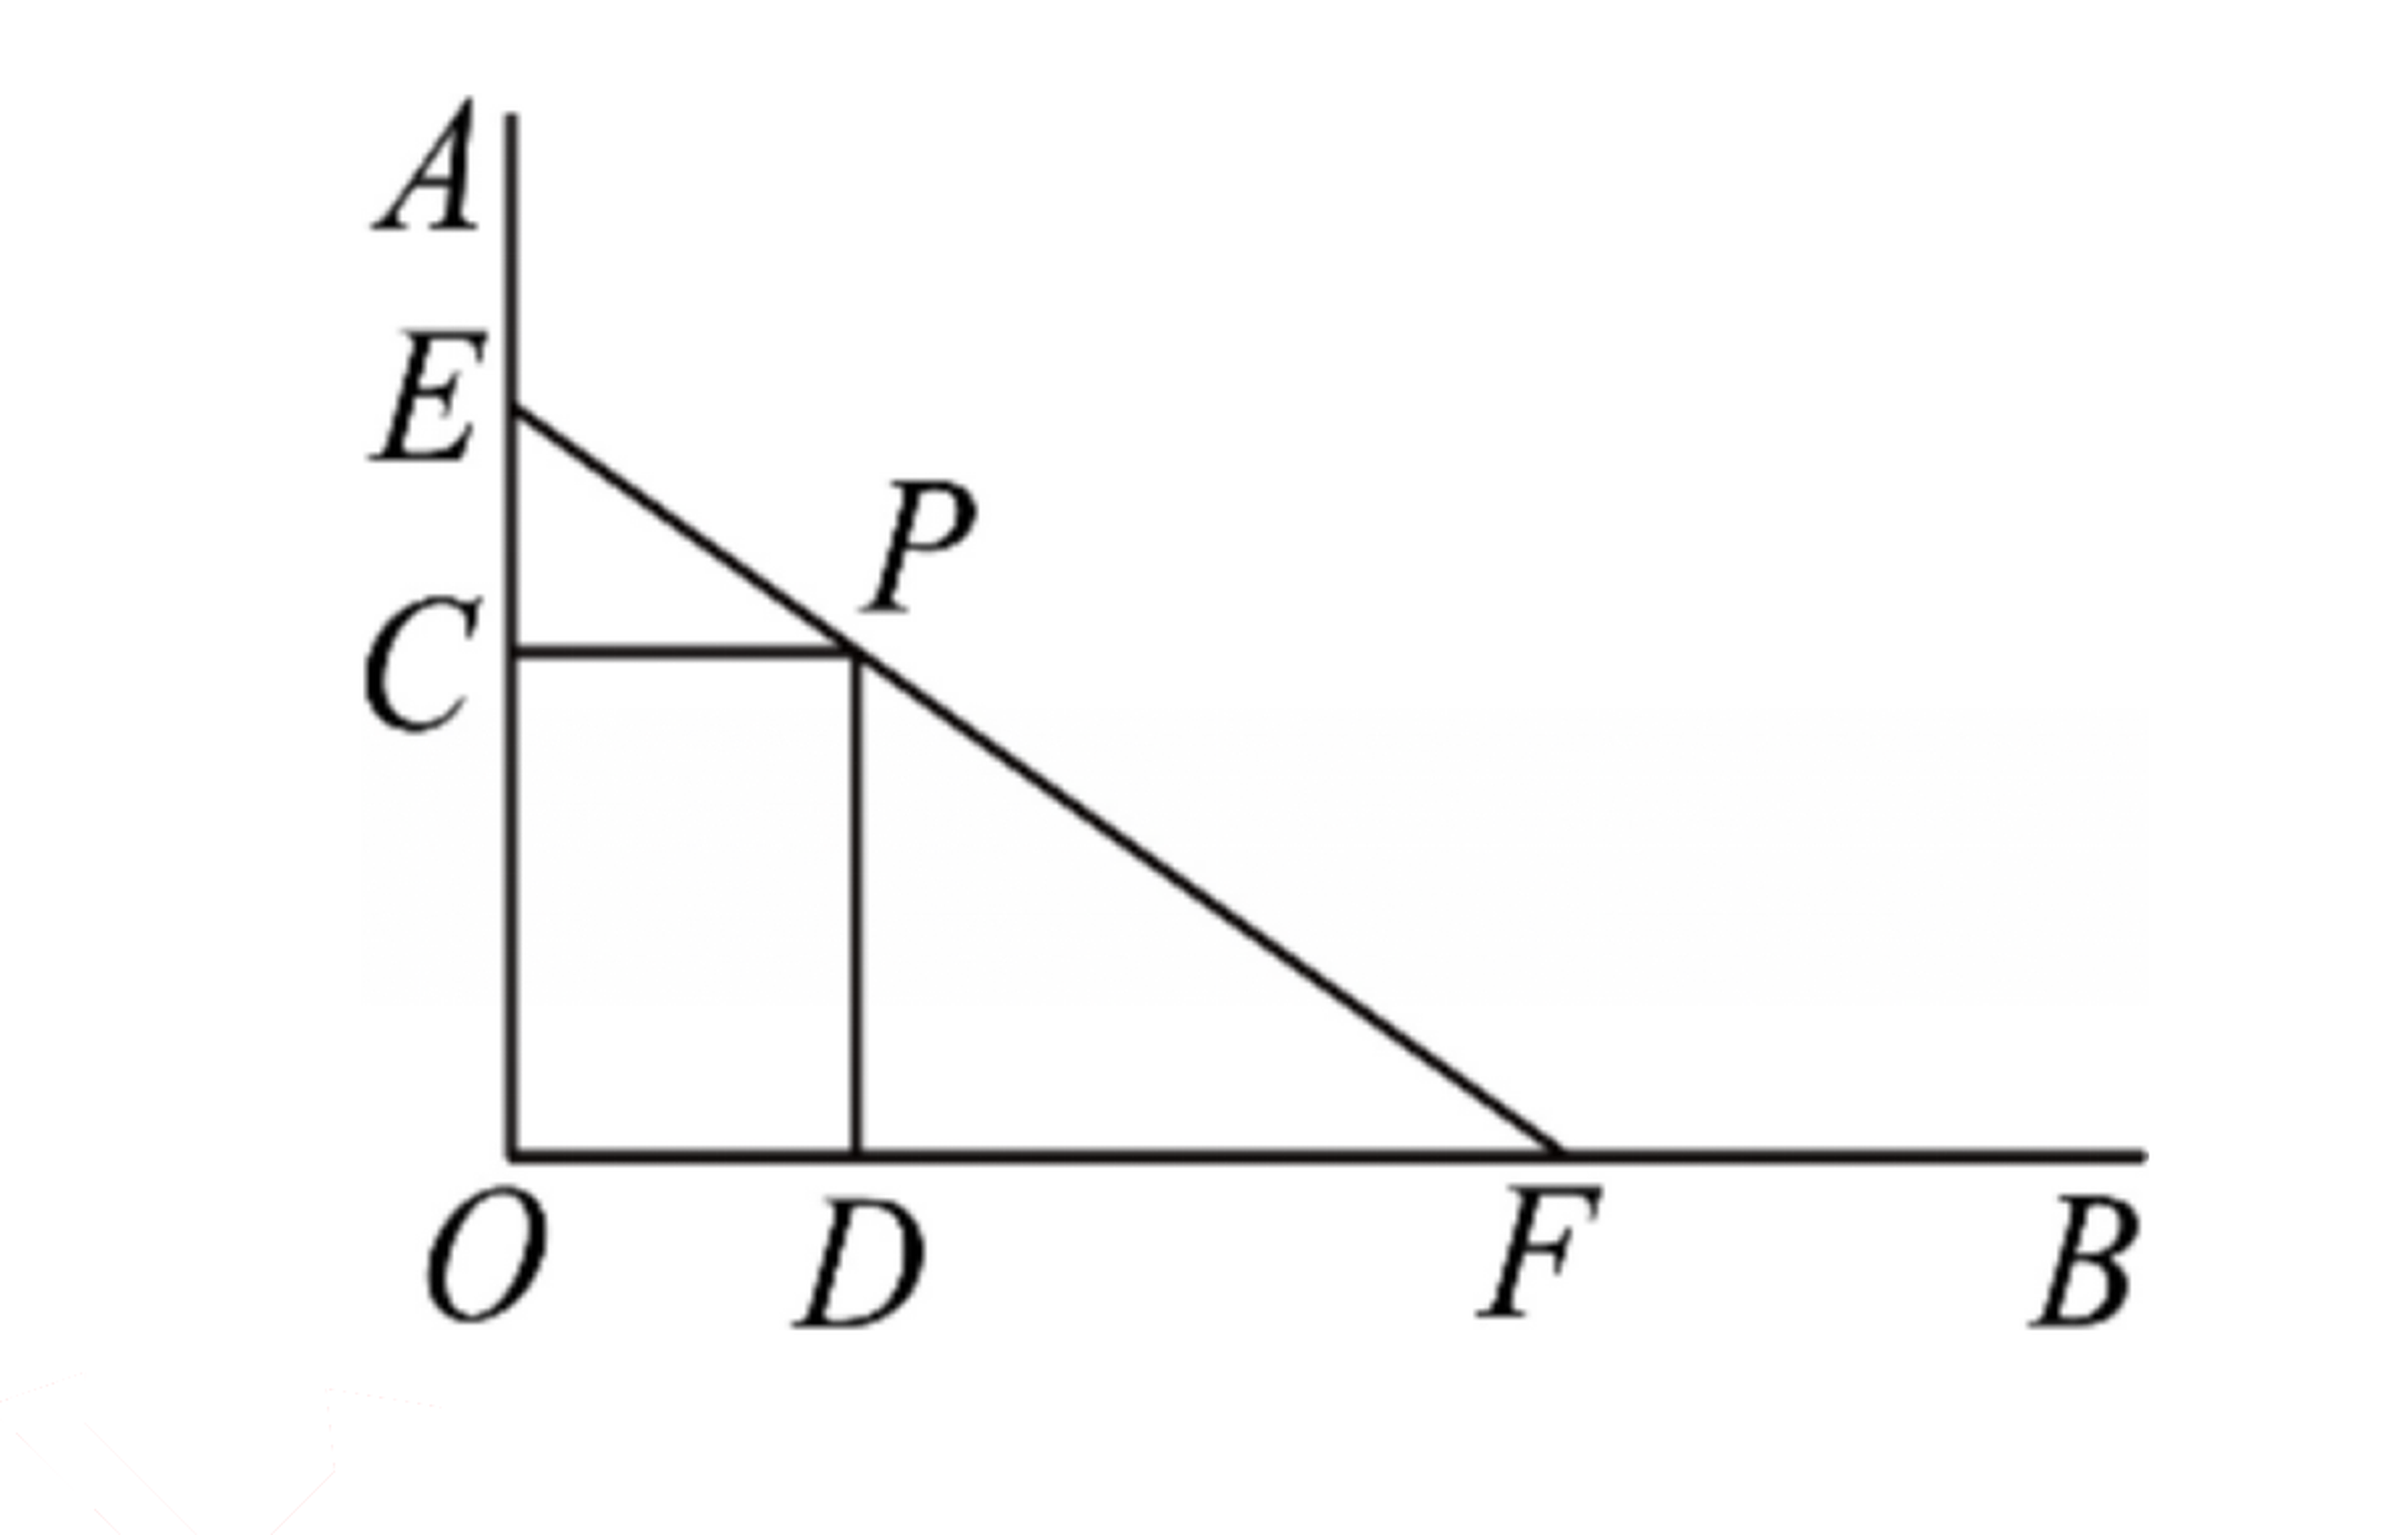
\includegraphics[width=0.32\textwidth]{figures/gao131_q19.png}
\end{center}

\ifanswer
\solbegin
\step{(1) 由题意得 $x\leq60$，}
\step{$\triangle PCE\sim\triangle FDP$，所以 $\dfrac{EC}{CP}=\dfrac{PD}{DF}$，即 $\dfrac{x}{25}=\dfrac{40}{DF}$，得 $DF=\dfrac{1000}{x}$m，}
\step{所以 $OF=OD+DF=\left(25+\dfrac{1000}{x}\right)$m，}
\step{所以 $25+\dfrac{1000}{x}\leq100$，解得 $x\geq\dfrac{40}{3}$；}
\step{综上，$\dfrac{40}{3}\leq x\leq60$；}
\step{(2) 由 $OE=OC+CE=(40+x)$m，}
\step{所以 $S=\dfrac12 OF\cdot OE=\dfrac12\left(25+\dfrac{1000}{x}\right)(40+x)$}
\step{$=\dfrac12\left(1000+25x+\dfrac{40000}{x}+1000\right)$m$^2$，}
\step{由基本不等式得 $S\geq\dfrac12\left(2000+2\sqrt{25x\cdot\dfrac{40000}{x}}\right)=2000$m$^2$，}
\step{当且仅当 $25x=\dfrac{40000}{x}$，即 $x=40$ 时取等号，}
\step{故 $EC=40$m 时，$S$ 取得最小值，为 $2000$m$^2$.}
\solend
\fi

\item 已知 $a\in\R$，函数 $y=ax^2+(3a+2)x+2a+3$.

(1) 当 $a=1$ 时，函数 $y=ax^2+(3a+2)x+2a+3$ 的图象与 $x$ 轴交于 $A(x_1,0)$，$B(x_2,0)$ 两点，求 $x_1^3+x_2^3$；

(2) 若关于 $x$ 的不等式 $ax^2+(3a+2)x+2a+3>2x$ 的解集为 $\R$，求实数 $a$ 的取值范围；

(3) 求关于 $x$ 的不等式 $y\geq1$ 的解集.

\ifanswer
\solbegin
\step{(1) 函数 $y=ax^2+(3a+2)x+2a+3$，当 $a=1$ 时，$y=x^2+5x+5$，}
\step{因为 $y=x^2+5x+5$ 的图象与 $x$ 轴交于 $A(x_1,0)$，$B(x_2,0)$ 两点，}
\step{即 $x^2+5x+5=0$ 的两个根为 $x_1$、$x_2$，}
\step{由根与系数的关系得 $x_1+x_2=-5$，$x_1x_2=5$，}
\step{所以 $x_1^2+x_2^2=(x_1+x_2)^2-2x_1x_2=25-10=15$，}
\step{所以 $x_1^3+x_2^3=(x_1+x_2)(x_1^2+x_2^2-x_1x_2)=-5\times(15-5)=-50$；}
\step{(2) 不等式 $ax^2+(3a+2)x+2a+3>2x$ 恒成立，得 $ax^2+3ax+2a+3>0$.}
\step{当 $a=0$ 时，$3>0$，恒成立，符合题意；}
\step{当 $a\neq0$ 时，若 $a<0$，二次函数 $ax^2+3ax+2a+3$ 开口向下，}
\step{一定存在小于零的部分，故不满足题意；}
\step{当 $a>0$ 时，若使 $ax^2+3ax+2a+3>0$ 恒成立，}
\step{只需 $\Delta=(3a)^2-4\times a\times(2a+3)=a^2-12a<0$，解得 $0<a<12$，}
\step{综上所述，$a$ 的取值范围为 $0\leq a<12$.}
\step{(3) 由 $y\geq1$，得 $ax^2+(3a+2)x+2a+3\geq1$，}
\step{即 $ax^2+(3a+2)x+2a+2\geq0$，即 $(ax+2a+2)(x+1)\geq0$，}
\step{当 $a=0$ 时，$2x+2\geq0$，解得 $x\geq-1$，}
\step{当 $a\neq0$ 时，}
\step{方程 $ax^2+(3a+2)x+2a+2=0$ 即为 $(x+1)(ax+2a+2)=0$，}
\step{解得 $x=-1$ 或 $x=-2-\dfrac2a$，令 $-1=-2-\dfrac2a$，即 $a=-2$，}
\step{当 $a>0$ 时，$-2-\dfrac2a<-1$，}
\step{不等式 $ax^2+(3a+2)x+2a+2\geq0$ 即为 $\left(x+\dfrac{2a+2}a\right)(x+1)\geq0$，}
\step{解得 $x\leq-2-\dfrac2a$ 或 $x\geq-1$；}
\step{当 $a<0$ 时，当 $-2-\dfrac2a<-1$，即 $a<-2$ 时，}
\step{不等式 $ax^2+(3a+2)x+2a+2\geq0$，即为 $\left(x+\dfrac{2a+2}a\right)(x+1)\leq0$，}
\step{解得 $-2-\dfrac2a\leq x\leq-1$；}
\step{当 $-2-\dfrac2a=-1$，即 $a=-2$，}
\step{不等式 $ax^2+(3a+2)x+2a+2\geq0$ 即为 $-2x^2-4x-2\geq0$，解得 $x=-1$，}
\step{当 $-2-\dfrac2a>-1$，即 $-2<a<0$ 时，}
\step{不等式 $ax^2+(3a+2)x+2a+2\geq0$ 即为 $\left(x+\dfrac{2a+2}a\right)(x+1)\leq0$，}
\step{解得 $-1\leq x\leq-2-\dfrac2a$，}
\step{综上所述，当 $a=0$ 时，解集为 $\{x\mid x\geq-1\}$；}
\step{当 $a>0$ 时，解集为 $\{x\mid x\leq-2-\dfrac2a$ 或 $x\geq-1\}$；}
\step{当 $a<-2$ 时，解集为 $\{x\mid -2-\dfrac2a\leq x\leq-1\}$；}
\step{当 $a=-2$ 时，解集为 $\{x\mid x=-1\}$；}
\step{当 $-2<a<0$ 时，解集为 $\{x\mid -1\leq x\leq-2-\dfrac2a\}$.}
\solend
\fi

\item 仔细阅读以下材料：【已知 $a$、$b\in(0,+\infty)$，$a+b=1$，求 $y=\dfrac1a+\dfrac2b$ 的最小值.

$y=\dfrac1a+\dfrac2b=\left(\dfrac1a+\dfrac2b\right)(a+b)=\dfrac ba+\dfrac{2a}b+3\geq3+2\sqrt2$，当且仅当 $\dfrac ba=\dfrac{2a}b$，即 $a=\sqrt2-1$，$b=2-\sqrt2$ 时取得等号，则 $y=\dfrac1a+\dfrac2b$ 的最小值为 $3+2\sqrt2$.

另 $y=\dfrac1a+\dfrac2b=\dfrac{a+b}a+\dfrac{2(a+b)}b=\dfrac ba+\dfrac{2a}b+3\geq3+2\sqrt2$，当且仅当 $\dfrac ba=\dfrac{2a}b$，即 $a=\sqrt2-1$，$b=2-\sqrt2$ 时取得等号，则 $y=\dfrac1a+\dfrac2b$ 的最小值为 $3+2\sqrt2$.】参考上述解法，求解下列问题.

(1) 若正实数 $x$、$y$ 满足 $x+y=1$，求 $\dfrac2x+\dfrac3y$ 的最小值；

(2) 已知 $x\in\left(0,\dfrac12\right)$，求 $t=\dfrac1x+\dfrac8{1-2x}$ 的最小值，并写出此时 $x$ 的值；

(3) 已知 $a$、$b\in(0,+\infty)$，$a+2b=1$，求 $p=\dfrac1{3a+4b}+\dfrac1{a+3b}$ 的最小值.

\ifanswer
\solbegin
\step{(1) 因为 $x>0,y>0$，且 $x+y=1$，}
\step{所以 $\dfrac2x+\dfrac3y=\left(\dfrac2x+\dfrac3y\right)(x+y)=2+\dfrac{2y}x+\dfrac{3x}y+3=5+\dfrac{2y}x+\dfrac{3x}y$，}
\step{由基本不等式得 $\dfrac{2y}x+\dfrac{3x}y\geq2\sqrt{\dfrac{2y}x\cdot\dfrac{3x}y}=2\sqrt6$，}
\step{当且仅当 $\dfrac{2y}x=\dfrac{3x}y$，即 $2y^2=3x^2$ 时，等号成立，}
\step{又因为 $x>0,y>0$ 且 $x+y=1$，此时 $x=\sqrt6-2,y=3-\sqrt6$，}
\step{所以 $\dfrac2x+\dfrac3y\geq5+2\sqrt6$，故 $\dfrac2x+\dfrac3y$ 的最小值为 $5+2\sqrt6$.}
\step{(2) 由 $0<x<\dfrac12$，则 $t=\dfrac1x+\dfrac8{1-2x}=\dfrac{2(1-2x+2x)}{2x}+\dfrac{8(1-2x+2x)}{1-2x}$}
\step{$=10+\dfrac{2\cdot(1-2x)}{2x}+\dfrac{8\cdot2x}{1-2x}\geq10+2\sqrt{\dfrac{2\cdot(1-2x)}{2x}\cdot\dfrac{8\cdot2x}{1-2x}}=18$，}
\step{当且仅当 $\dfrac{2\cdot(1-2x)}{2x}=\dfrac{8\cdot2x}{1-2x}$，即 $x=\dfrac16$ 时等号成立；}
\step{(3) 由 $a$、$b>0$，$a+2b=1$，则 $a=1-2b>0$，即 $0<b<\dfrac12$，}
\step{所以 $p=\dfrac1{3a+4b}+\dfrac1{a+3b}=\dfrac1{3a+6b-2b}+\dfrac1{a+2b+b}=\dfrac1{3-2b}+\dfrac1{1+b}$}
\step{$=\dfrac1{3-2b}+\dfrac2{2+2b}$，显然 $3-2b$、$2+2b>0$，}
\step{所以 $p=\dfrac15\cdot(3-2b+2+2b)\cdot\left(\dfrac1{3-2b}+\dfrac2{2+2b}\right)=\dfrac15\left[3+\dfrac{2+2b}{3-2b}+\dfrac{2(3-2b)}{2+2b}\right]$}
\step{$\geq\dfrac15\left[3+2\sqrt{\dfrac{2+2b}{3-2b}\cdot\dfrac{2(3-2b)}{2+2b}}\right]=\dfrac{3+2\sqrt2}5$，}
\step{当且仅当 $\dfrac{2+2b}{3-2b}=\dfrac{2(3-2b)}{2+2b}$，}
\step{即 $b=\dfrac{8-5\sqrt2}2$，$a=5\sqrt2-7$ 时等号成立.}
\solend
\fi

\end{enumerate}

\end{document}
"
% 紧凑版：xelatex "\def\iscompact{1}% 高一131_六十中学_期中.tex
%   —— 高一上数学"2026-2027 年六十中学高一上期中"（试卷版/答案版）
% 试卷版：xelatex 高一131_六十中学_期中.tex
% 答案版：xelatex "\def\isanswer{1}\input{高一131_六十中学_期中.tex}"
% 紧凑版：xelatex "\def\iscompact{1}\input{高一131_六十中学_期中.tex}"
%
% 原始材料：微信公众号"魔都数学加油站"文章，作者破晓，2026-11-13 18:18 发布；
% 连载"27学年高一131"，原文标题"27学年高一131——2026-2027年上海市六十中学高一上期中"；
% 原文链接：https://mp.weixin.qq.com/s/Nrbp3Uvt-sOGnOp4MEHemA。
% 正文为 11 张 PNG 页（01—05、09—11 为 2560x3620，06—08 为 4762x6735），
% 题目下印有【解析】或【答案】，为讲评版。题目、解析均据原图转录；
% 卷面粉红色水印"魔都数学加油站"及公众号页脚未录入。全卷仅第 19 题有 1 幅插图
% （矩形 OCPD 与小路 EF 的示意图），取 07.png 截图去水印。
%
% 卷首标题：原卷印作"2026-2027 年六十中学高一上期中"（公众号标题中的"上海市"
% 卷面标题行没有，本稿照卷面），年份区间按全稿惯例排 en dash；原卷未印副标题，
% 本卷为期中卷、跨集合与常用逻辑用语／不等式／函数三章，按题目内容标为
% "集合与常用逻辑用语、不等式、函数"（与 125／126／128／129 同期中卷口径相同）：
% 集合与逻辑见 Q3、Q4、Q7、Q13、Q17，不等式见 Q8、Q10、Q12、Q14、Q15、Q16、Q19、
% Q20、Q21，函数（指数／对数／幂函数、基本不等式应用）见 Q5、Q6、Q9、Q11、Q18、Q21。
%
% 题号体例：本卷共 19 题——一、填空题 3—12（10 题）、二、选择题 13—16（4 题）、
% 三、解答题 17—21（5 题）。三节分别 \setcounter{enumi}{2}／{12}／{16}。
%
% 与原卷的排版差异：
%   ① 原文从第 3 题起，本稿保留原题号（见上"题号体例"）；
%   ② 原卷每题下直接印【解析】／【答案】，本稿按全稿惯例置于答案版；第 3、4 题只印
%      【答案】，另提 \ans{}；第 13—16 题答案在解析末句"故选 …"，题干括号内留空、
%      不另提 \ans{}；其余各题印【解析】、无独立答案段；
%   ③ 原卷未印副标题，本稿按"知识模块"口径补出；
%   ④ 原卷填空横线按全稿惯例排为 \blankline[4.4em]；选择题括号排 \mbox{（\quad）}、
%      选项段前按惯例加 \keepwithprev；解答题不留作答区（原卷为讲评版，与 109—129 同）；
%   ⑤ 原卷数集排斜体 $R$／$N$，按全稿惯例改 \R／\N；绝对值排 \lvert…\rvert，
%      集合描述竖线排 \mid；不等号按全稿惯例排 \leqslant／\geqslant；
%   ⑥ 子题标号 (1)(2)(3) 原卷用半角括号，照录；圈数字 ①② 照录；
%   ⑦ 原卷第 19 题插图浮排在第 07 页题干右侧，本稿按体例就近置于题干"如图"之后
%      （居中 \includegraphics），图取原卷 07 页截图去水印；题前按惯例加
%      \needvspace{7cm} 守卫（照 高一120／127／129 成例），保证"题干 + 图"整块不被页边界切开；
%   ⑧ 原卷 Q9 题干跨 01—02 页、Q15 解析跨 03—04 页、Q16 材料跨 04—05 页、
%      Q17 题干跨 05—06 页、Q20 解析跨 08—09 页、Q21 解析跨 09—11 页，
%      本稿按题合并连续排版；末页第 11 页为 Q21 (3) 解析的续尾，按实际印刷行单列。
%   ⑨ 第 16 题材料英文括注原卷印作 (Cauchy – SchwarzInequality)（长横、Schwarz 与
%      Inequality 斜体连排无空格），本稿按全稿英文专名惯例排 \emph{(Cauchy-Schwarz Inequality)}；
%      第 15 题解析 B、D 两行原卷各印一步含 \lg m 的换底繁分数（2026-11-13 回原图核对补回，
%      本稿初转曾顺手去重跳过该步）。
%
% 判别式字形：第 20 题 (2) 解析 $\Delta=(3a)^2-4\times a\times(2a+3)=a^2-12a<0$
%   原卷排三角形（等腰、高；回 08.png 放大核对），照录 \Delta；全卷判别式仅此一处
%   （\triangle 另作第 19 题「$\triangle PCE\sim\triangle FDP$」的几何三角形记号）。
%
% 子集符号：第 17 题 (2) 解析 $P\subseteq Q$ 印带下划线，照录 \subseteq；
%   全卷未出现单线 \subset。
%
% 原卷存疑照录：
%   第 11 题解析末两式作 $\dfrac{2+m+\frac1n}{2n+2}=\dfrac{2n+mn+1}{2n+2}$，而第三式
%     分母 $\log_3 9+\log_3 2+\log_3 2=2+\frac2n$，与前一分母 $2n+2$ 不等，照录；
%   第 16 题材料 ①"对于所有实数 $x$ 和 $y$，有 $(a^2+b^2)(c^2+d^2)\geq(ac+bd)^2$"
%     句首用 $x$、$y$ 而式中用 $a$、$b$、$c$、$d$，照录；
%   第 20 题题干 (2) 作"解集为 $\R$"、解析 (2) 作"恒成立"，措辞不同，照录；
%   第 21 题材料把同一道题用两种解法连印两遍（"另 $y=\frac1a+\frac2b=\dots$"），照录；
%   第 21 题 (3) 解析末句"即 $b=\frac{8-5\sqrt2}{2}$，$a=5\sqrt2-7$ 时等号成立"
%     未另写"故最小值为 $\frac{3+2\sqrt2}{5}$"，照录；
%   第 12 题解析"所以 $e^a+e^b>e^c, a+b>c$"、第 8 题解析"$a>0$，$b>0$"、
%     第 18 题 (2)"$4x^2-4x+1<x^2+4x+4$，解得 $-\frac13<x<3$"等处数学式内
%     半角逗号，照录；
%   第 15 题解析用 $\lg$ 记常用对数（$\lg m$、$\lg 3$、$\lg 5$、$\lg 15$），照录。
%
% 行数复核：逐题数 \step 条数，合计 119 条（Q3：0；Q4：0；Q5：1；Q6：1；Q7：2；
% Q8：2；Q9：1；Q10：1；Q11：2；Q12：6；Q13：2；Q14：3；Q15：14；Q16：10；
% Q17：4；Q18：8；Q19：11；Q20：35；Q21：16），与原卷印刷行逐题相等
% （cases 块作一个印刷行计）。第 3、4 题只印【答案】，提 \ans{}，不计入 \step 账；
% 四道选择题答案均在解析末句，括号内留空、不另提 \ans{}。
%
\documentclass[a4paper,11pt]{article}
\usepackage{common}

\begin{document}

\examtitlest[3]{2026--2027 年六十中学高一上期中}{集合与常用逻辑用语、不等式、函数}

\bigsec{一、填空题}

\begin{enumerate}
\setcounter{enumi}{2}

\item 已知集合 $A=(0,4),B=[2,5]$，则 $A\cup B=$\blankline[4.4em].

\ifanswer
\ans{$(0,5]$}
\fi

\item 陈述句“$x=2$ 或 $y=3$”的否定形式为\blankline[4.4em].

\ifanswer
\ans{$x\neq2$ 且 $y\neq3$}
\fi

\item 函数 $y=a^{x-2}+15(a>0$ 且 $a\neq1)$ 的图象恒过定点的坐标为\blankline[4.4em].

\ifanswer
\solbegin
\step{函数 $y=a^{x-2}+15$ 的图象恒过定点 $A(2,16)$.}
\solend
\fi

\item 用有理数指数幂的形式来化简：$\dfrac{\sqrt{a\cdot\sqrt[3]{a^4}}}{\left(a^{\frac13}\right)^2}=$\blankline[4.4em].

\ifanswer
\solbegin
\step{原式 $=\dfrac{\sqrt{a\cdot a^{\frac43}}}{a^{\frac23}}=\dfrac{\sqrt{a^{\frac73}}}{a^{\frac23}}=\dfrac{a^{\frac76}}{a^{\frac23}}=a^{\frac76-\frac23}=a^{\frac12}(a>0)$.}
\solend
\fi

\item 已知集合 $A=\left\{x\mid \dfrac6{6-x}\in\N\text{ 且 }x\in\N\right\}$，则用列举法表示集合 $A=$\blankline[4.4em].

\ifanswer
\solbegin
\step{当 $x=0$ 时，$\dfrac6{6-0}=1\in\N$，当 $x=3$ 时，$\dfrac6{6-3}=2\in\N$，}
\step{当 $x=4$ 时，$\dfrac6{6-4}=3\in\N$，当 $x=5$ 时，$\dfrac6{6-5}=6\in\N$，故 $A=\{0,3,4,5\}$.}
\solend
\fi

\item 已知 $a>0$，$b>0$，且 $ab=\dfrac12$，则 $\dfrac1a+\dfrac8b$ 的最小值是\blankline[4.4em].

\ifanswer
\solbegin
\step{$a>0$，$b>0$，且 $ab=\dfrac12$，则 $\dfrac1a+\dfrac8b\geq2\sqrt{\dfrac8{ab}}=8$，}
\step{当且仅当 $\dfrac1a=\dfrac8b$，即 $a=\dfrac14,b=2$ 时取等号，故最小值为 $8$.}
\solend
\fi

\item 心理学家有时用函数 $L(t)=A(1-e^{-kt})$ 测定在时间 $t$（单位：$min$）内能够记忆的量 $L$，其中 $A$ 表示需要记忆的量，$k$ 表示记忆率. 假设一个学生需要记忆的量为 $200$ 个单词，此时 $L$ 表示在时间 $t$ 内该生能够记忆的单词个数. 已知该生在 $5min$ 内能够记忆 $20$ 个单词，则 $k$ 的值约为\blankline[4.4em]（结果保留四位小数）.

\ifanswer
\solbegin
\step{由题意得 $200(1-e^{-5k})=20$，所以 $e^{-5k}=0.9$，解得 $k\approx0.0211$.}
\solend
\fi

\item 设 $x\in\R$，方程 $\lvert 3x-2\rvert+\lvert 1-x\rvert=\lvert 2x-1\rvert$ 的解集是\blankline[4.4em].

\ifanswer
\solbegin
\step{由三角不等式得 $(3x-2)(1-x)\geq0$，故解集是 $\left[\dfrac23,1\right]$.}
\solend
\fi

\item 已知 $3^m=5$，$n=\log_2 3$，则 $\log_{36}90$ 可用 $m$、$n$ 表示为\blankline[4.4em].

\ifanswer
\solbegin
\step{由 $3^m=5$，又 $n=\log_2 3$，得 $m=\log_3 5$，$\log_3 2=\dfrac{\log_2 2}{\log_2 3}=\dfrac1n$，}
\step{所以 $\log_{36}90=\dfrac{\log_3 90}{\log_3 36}=\dfrac{\log_3 9+\log_3 2+\log_3 5}{\log_3 9+\log_3 2+\log_3 2}=\dfrac{2+m+\frac1n}{2n+2}=\dfrac{2n+mn+1}{2n+2}$.}
\solend
\fi

\item 若定义域为 $I=(0,m]$ 的函数 $f(x)=e^x$ 满足：对任意能构成三角形三边长的实数 $a$、$b$、$c\in I$，均有 $f(a)$、$f(b)$、$f(c)$ 也能构成三角形三边长，则 $m$ 的最大值为\blankline[4.4em].

\ifanswer
\solbegin
\step{$f(x)=e^x$ 在 $I=(0,m]$ 上严格增，所以 $f(x)\in(1,e^m]$，不妨设 $0<a\leq b\leq c$，}
\step{因为对任意能构成三角形三边长的实数 $a,b,c\in I$，均有 $f(a)$，$f(b)$，$f(c)$}
\step{也能构成三角形三边长，所以 $e^a+e^b>e^c, a+b>c$，}
\step{因为 $e^a+e^b\geq2\sqrt{e^ae^b}=2\sqrt{e^{a+b}}>e^c$，所以 $4e^{a+b}>e^{2c}$，}
\step{因为对任意 $a,b,c\in I$ 都成立，所以 $4e^c\geq e^{2c}$，所以 $e^c\leq4$，所以 $c\leq\ln4$，}
\step{所以 $m\leq\ln4$，所以 $m$ 的最大值为 $\ln4$.}
\solend
\fi

\end{enumerate}

\bigsec{二、选择题}

\begin{enumerate}
\setcounter{enumi}{12}

\item 已知 $m,n$ 是非零自然数，命题 $\alpha:mn$ 是奇数，命题 $\beta:m$ 或 $n$ 是奇数，则 $\alpha$ 是 $\beta$ 的\mbox{（\quad）}

\keepwithprev
A. 充分非必要条件\qquad\qquad B. 必要非充分条件

C. 充要条件\qquad\qquad D. 既非充分又非必要条件

\ifanswer
\solbegin
\step{$mn$ 是奇数 $\Leftrightarrow$ $m$、$n$ 都是奇数，所以 $\alpha$ 能推出 $\beta$，充分性成立，}
\step{但 $\beta$ 推不出 $\alpha$，必要性不成立，所以 $\alpha$ 是 $\beta$ 的充分非必要条件. 故选 $A$.}
\solend
\fi

\item 关于 $x$ 的不等式 $x^2-mx+n+5\leq0$ 的解集是 $[1,8]$，那么 $\log_m n=$\mbox{（\quad）}

\keepwithprev
A. $\dfrac13$\qquad\qquad B. $-3$\qquad\qquad C. $-2$\qquad\qquad D. $\dfrac12$

\ifanswer
\solbegin
\step{由题意得 $x^2-mx+n+5=0$ 的解为 $1$，$8$，}
\step{由根与系数的关系得 $\begin{cases}1+8=m\\1\times8=n+5\end{cases}$，解得 $m=9$，$n=3$，}
\step{所以 $\log_m n=\log_9 3=\dfrac12\log_3 3=\dfrac12$. 故选 $D$.}
\solend
\fi

\item 已知正实数 $x$、$y$、$z$ 满足 $3^x=5^y=15^z$，则下列说法中不正确的是\mbox{（\quad）}

\keepwithprev
A. $\dfrac1x+\dfrac1y=\dfrac1z$\qquad\qquad B. $x+y>2z$\qquad\qquad C. $3x>5y>15z$\qquad\qquad D. $x\cdot y>4z^2$

\ifanswer
\solbegin
\step{已知正实数 $x$、$y$、$z$，则设 $3^x=5^y=15^z=m>1$，}
\step{所以 $x=\log_3 m$，$y=\log_5 m$，$z=\log_{15} m$，}
\step{对于 $A$，$\dfrac1x+\dfrac1y=\dfrac1{\log_3 m}+\dfrac1{\log_5 m}=\log_m 3+\log_m 5=\log_m 15=\dfrac1z$，故 $A$ 正确；}
\step{对于 $B$，因为 $\dfrac{x+y}{z}=\dfrac{x}{z}+\dfrac{y}{z}=\dfrac{\log_3 m}{\log_{15} m}+\dfrac{\log_5 m}{\log_{15} m}=\dfrac{\dfrac{\lg m}{\lg3}}{\dfrac{\lg m}{\lg15}}+\dfrac{\dfrac{\lg m}{\lg5}}{\dfrac{\lg m}{\lg15}}=\dfrac{\lg15}{\lg3}+\dfrac{\lg15}{\lg5}$，}
\step{$=\dfrac{\lg3+\lg5}{\lg3}+\dfrac{\lg3+\lg5}{\lg5}=2+\dfrac{\lg5}{\lg3}+\dfrac{\lg3}{\lg5}=2+\log_3 5+\log_5 3$，}
\step{又 $\log_3 5>0$，$\log_5 3>0$，所以 $2+\log_3 5+\log_5 3>2$，}
\step{所以 $\dfrac{x+y}{z}>2$，即 $x+y>2z$，故 $B$ 正确；}
\step{对于 $C$，因为 $\dfrac5x=5\log_m 3=\log_m 243$，$\dfrac3y=3\log_m 5=\log_m 125$，}
\step{所以 $\dfrac5x>\dfrac3y$，即 $3x<5y$，故 $C$ 错误；}
\step{对于 $D$，$\dfrac{xy}{z^2}=\dfrac{x}{z}\cdot\dfrac{y}{z}=\dfrac{\log_3 m}{\log_{15} m}\cdot\dfrac{\log_5 m}{\log_{15} m}=\dfrac{\dfrac{\lg m}{\lg3}}{\dfrac{\lg m}{\lg15}}\cdot\dfrac{\dfrac{\lg m}{\lg5}}{\dfrac{\lg m}{\lg15}}=\dfrac{\lg15}{\lg3}\cdot\dfrac{\lg15}{\lg5}$}
\step{$=\dfrac{\lg3+\lg5}{\lg3}\cdot\dfrac{\lg3+\lg5}{\lg5}=\left(1+\dfrac{\lg5}{\lg3}\right)\left(1+\dfrac{\lg3}{\lg5}\right)=2+\dfrac{\lg5}{\lg3}+\dfrac{\lg3}{\lg5}$}
\step{$\geq2+2\sqrt{\dfrac{\lg5}{\lg3}\cdot\dfrac{\lg3}{\lg5}}=2+2=4$，又 $\lg3\neq\lg5$，故等号不成立，}
\step{所以 $\dfrac{xy}{z^2}>4$，即 $xy>4z^2$，故 $D$ 正确.}
\step{故选 $C$.}
\solend
\fi

\item 柯西不等式 \emph{(Cauchy-Schwarz Inequality)} 是一种在数学和物理学中广泛使用的不等式，它是由法国数学家奥古斯丁$\cdot$路易$\cdot$柯西提出的，柯西不等式可以用于证明其他不等式，也可以用于解决一些数学问题. 以下是柯西不等式的原始形式：

①对于所有实数 $x$ 和 $y$，有 $(a^2+b^2)(c^2+d^2)\geq(ac+bd)^2$.

②等式条件：当且仅当 $ad-bc=0$ 时，等号成立.

例：已知 $x+2y=2$，由柯西不等式 $(x^2+y^2)(1^2+2^2)\geq(x+2y)^2$，可得 $(x^2+y^2)_{min}=\dfrac45$.

现给出以下两个命题：

①若 $a^2+b^2=1$，则 $2a+3b$ 的最大值为 $\sqrt{13}$；

②若 $1<a<3$，则 $\sqrt{a-1}+\sqrt{6-2a}$ 的最大值为 $\sqrt6$；

则运用柯西不等式，判断以下正确的选项有\mbox{（\quad）}

\keepwithprev
A. ①为真命题；②为真命题\qquad\qquad B. ①为真命题；②为假命题

C. ①为假命题；②为真命题\qquad\qquad D. ①为假命题；②为假命题

\ifanswer
\solbegin
\step{由柯西不等式得 $(a^2+b^2)(2^2+3^2)\geq(2a+3b)^2$.}
\step{因为 $a^2+b^2=1$，所以 $(2^2+3^2)\geq(2a+3b)^2$，即 $13\geq(2a+3b)^2$，}
\step{所以 $-\sqrt{13}\leq2a+3b\leq\sqrt{13}$，则 $(2a+3b)_{max}=\sqrt{13}$，}
\step{当且仅当 $3a=2b$ 时取等号，故①正确.}
\step{令 $x=\sqrt{a-1}$，$y=\sqrt{3-a}$，则 $x^2+y^2=a-1+3-a=2$，}
\step{由柯西不等式得 $(\sqrt{a-1}+\sqrt{6-2a})^2=(\sqrt{a-1}+\sqrt2\cdot\sqrt{3-a})^2=(x+\sqrt2 y)^2$}
\step{$\leq[1^2+(\sqrt2)^2](x^2+y^2)$，}
\step{因为 $x^2+y^2=2$，所以 $(\sqrt{a-1}+\sqrt{6-2a})^2\leq6$，}
\step{当且仅当 $\sqrt{3-a}=\sqrt2\sqrt{a-1}$ 取等号，所以 $\sqrt{a-1}+\sqrt{6-2a}\leq\sqrt6$，故②正确.}
\step{故选 $A$.}
\solend
\fi

\end{enumerate}

\bigsec{三、解答题}

\begin{enumerate}
\setcounter{enumi}{16}

\item 已知集合 $P=\left\{x\mid \dfrac{3x-1}{x+2}<1\right\}$，集合 $Q=\{x\mid\lvert x-a\rvert\leq2\}$.

(1) 求集合 $P$；

(2) 若“$x\in P$”是“$x\in Q$”的充分非必要条件，求实数 $a$ 的取值范围.

\ifanswer
\solbegin
\step{(1) 集合 $P=\left\{x\mid \dfrac{3x-1}{x+2}<1\right\}$，得 $\dfrac{2x-3}{x+2}<0$，解得 $P=\left(-2,\dfrac32\right)$.}
\step{(2) 集合 $Q=\{x\mid\lvert x-a\rvert\leq2\}=\{x\mid a-2\leq x\leq2+a\}$，}
\step{由“$x\in P$”是“$x\in Q$”的充分非必要条件，得 $P\subseteq Q$，}
\step{得 $\begin{cases}-2\geq a-2\\\dfrac32\leq2+a\\a-2<2+a\end{cases}$，解得 $a\in\left[-\dfrac12,0\right]$.}
\solend
\fi

\item 已知幂函数 $f(x)=(m^2-4m+4)\cdot x^{2m-4}$ 在 $(-\infty,0)$ 上是严格减函数.

(1) 求函数 $y=f(x)$ 的解析式；

(2) 若 $f(1-2x)<f(x+2)$，求 $x$ 的取值范围.

\ifanswer
\solbegin
\step{(1) 由幂函数的定义得 $m^2-4m+4=1$，解得 $m=1$ 或 $3$，}
\step{当 $m=1$ 时，$f(x)=x^{-2}=\dfrac1{x^2}$，在 $(-\infty,0)$ 上严格增，不符合题意，}
\step{当 $m=3$ 时，$f(x)=x^2$，在 $(-\infty,0)$ 上严格减，符合题意，}
\step{所以 $f(x)=x^2$；}
\step{(2) 由函数 $f(x)=x^2$ 图象关于 $y$ 轴对称，且在 $[0,+\infty)$ 上严格增，}
\step{则 $f(1-2x)<f(x+2)$ 可化为 $\lvert1-2x\rvert<\lvert x+2\rvert$，}
\step{平方得 $4x^2-4x+1<x^2+4x+4$，解得 $-\dfrac13<x<3$，}
\step{所以 $x$ 的取值范围是 $\left(-\dfrac13,3\right)$.}
\solend
\fi

% 第 19 题是"题干 + 图"约 7cm 的一整块，守卫放在 \item 之前（放 \item 之后会失效）
\needvspace{7cm}
\item 如图，$OA$、$OB$ 是两条长度足够长的互相垂直的笔直小路，矩形 $OCPD$ 的顶点 $C$，$D$ 分别在 $OA$、$OB$ 上，且该矩形区域内种满了荷花. 为了让观赏者有更好的观赏体验，现计划经过点 $P$ 修一条小路 $EF$，其中点 $E$ 在小路 $OA$ 上，点 $F$ 在小路 $OB$ 上，并在 $\triangle OEF$ 区域内种满荷花. 已知 $OD=25m$，$OC=40m$，且小路 $EF$ 要完全位于一个以 $O$ 为顶点的，边长为 $100$ m 的正方形内部（包括边界）. 记 $\triangle OEF$ 的面积为 $S$m$^2$.

(1) 设 $EC=x\cdot m$，试用 $x$ 表示 $OF$，并求 $x$ 的取值范围.

(2) 当 $EC$ 的长度为多少时，$S$ 取得最小值？最小值是多少？

\begin{center}
% 图取原卷 07.png 截图去粉色水印，2.8× LANCZOS 放大
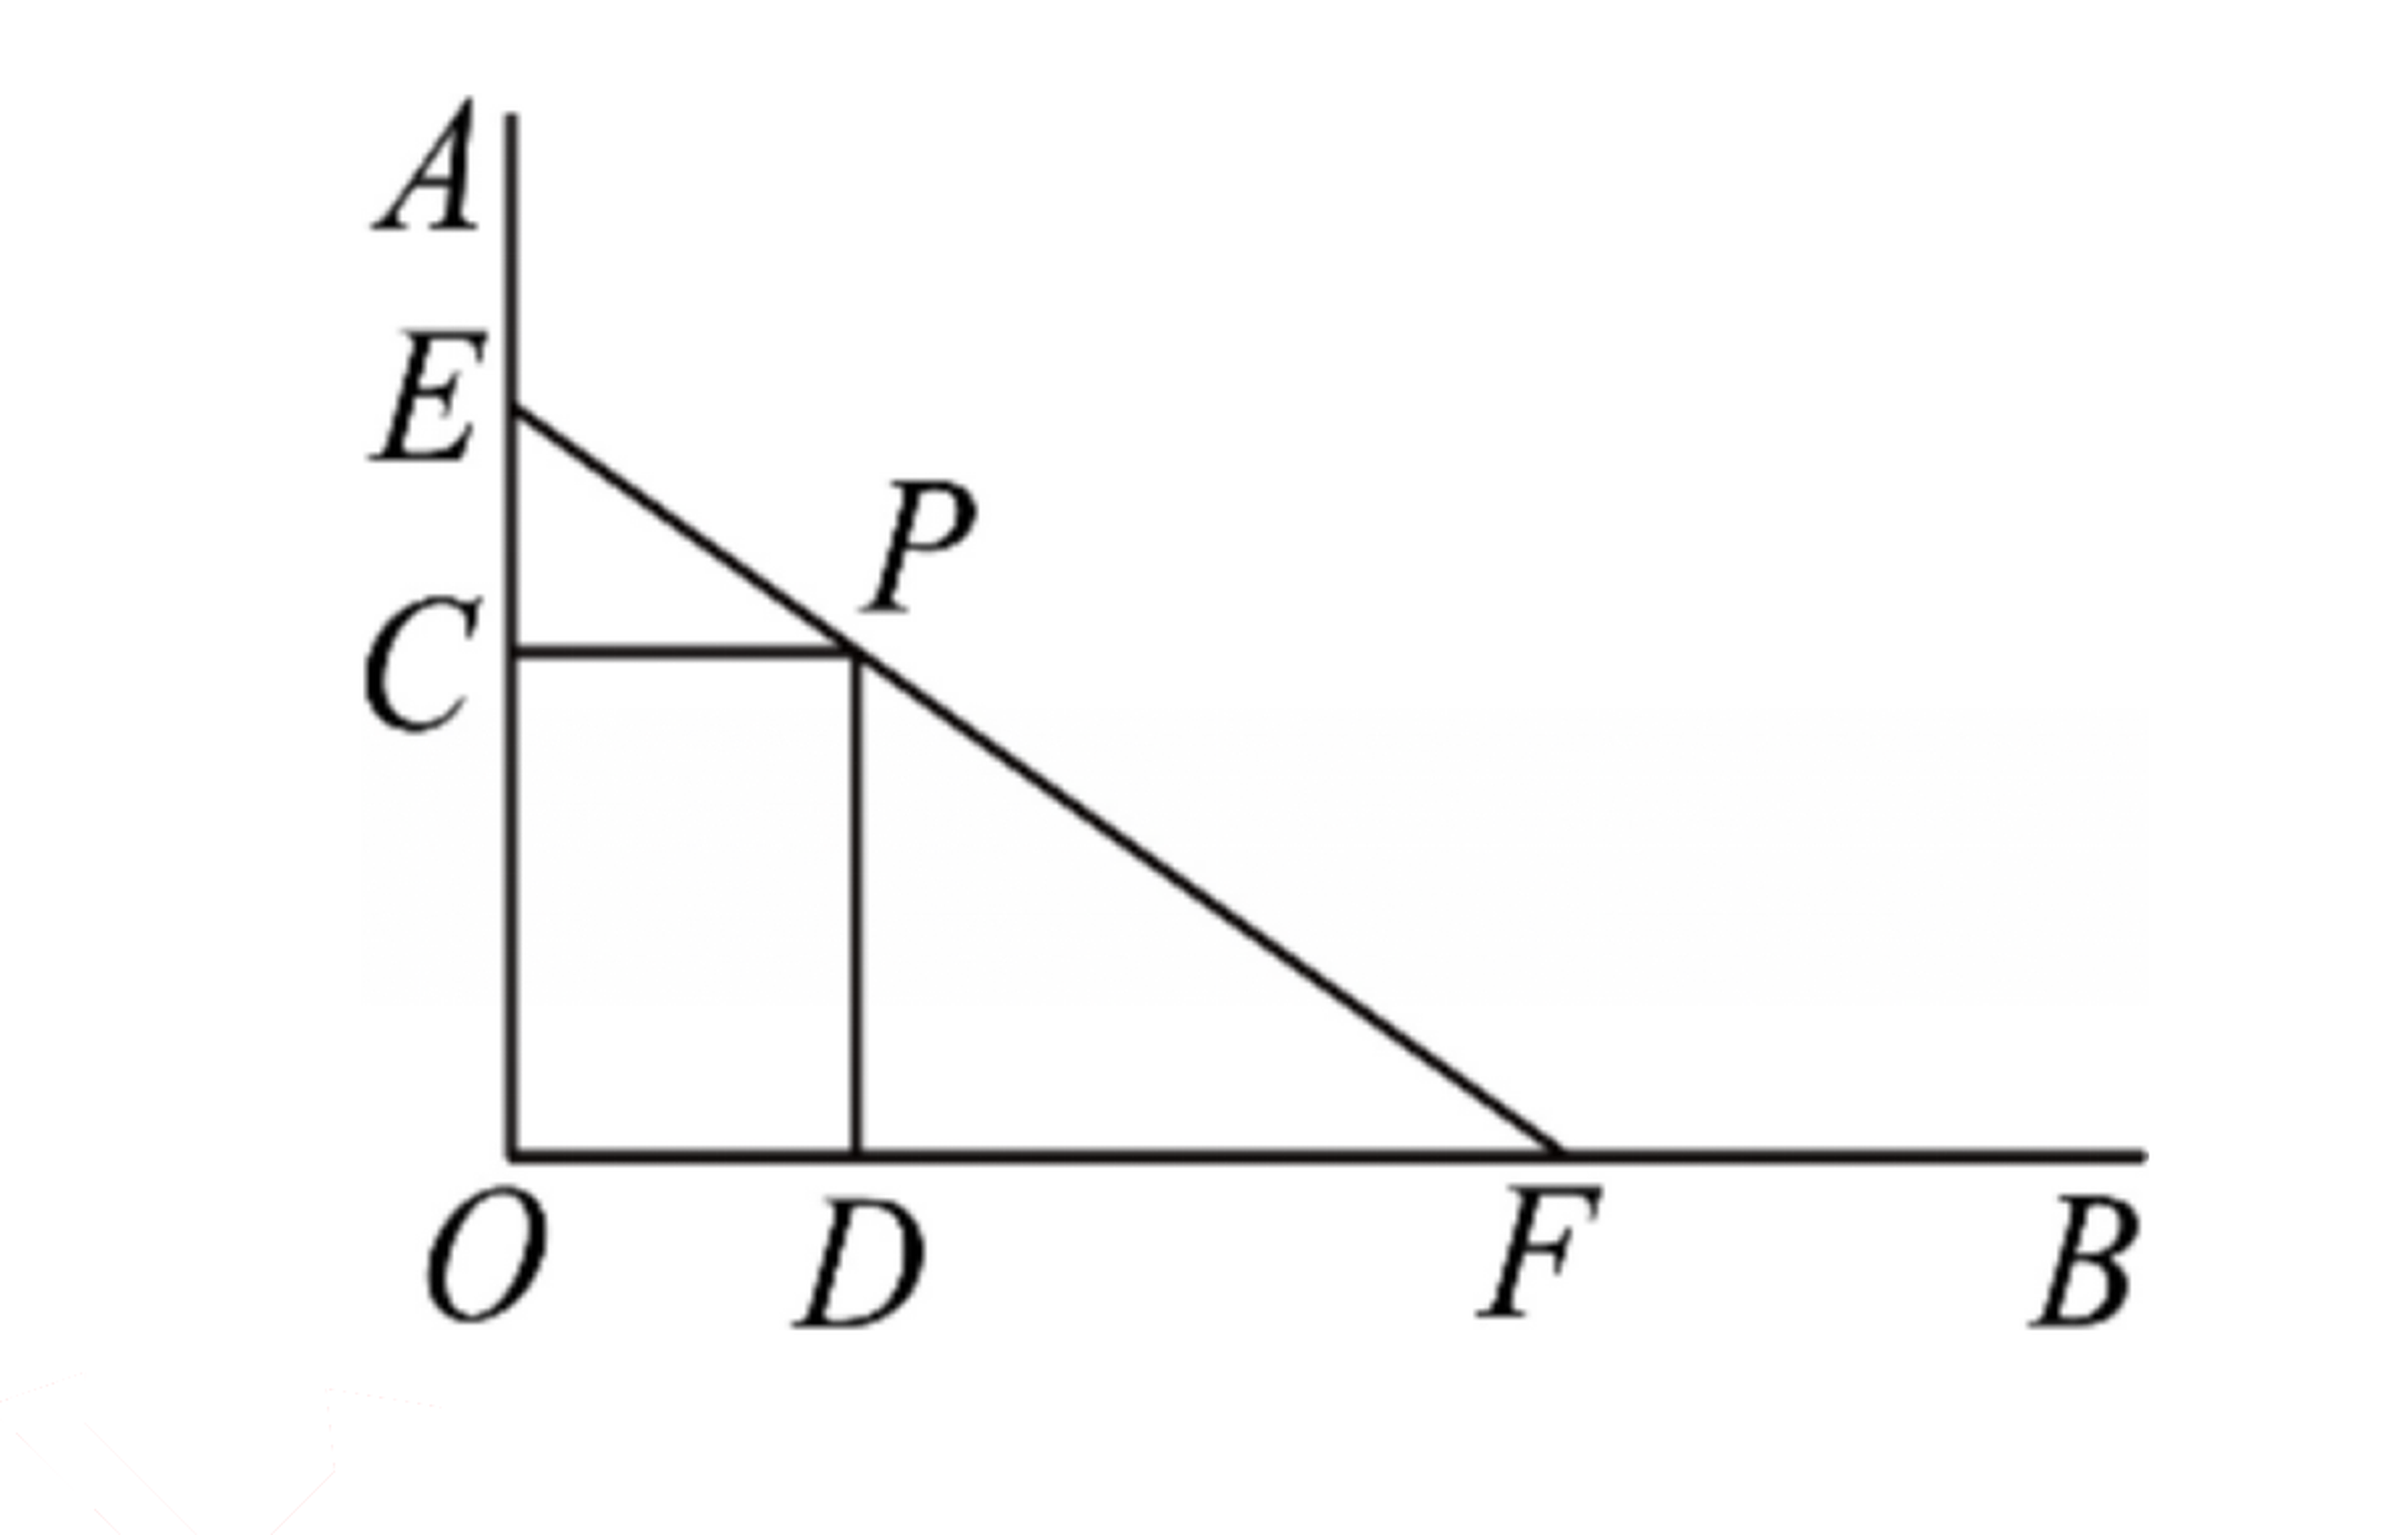
\includegraphics[width=0.32\textwidth]{figures/gao131_q19.png}
\end{center}

\ifanswer
\solbegin
\step{(1) 由题意得 $x\leq60$，}
\step{$\triangle PCE\sim\triangle FDP$，所以 $\dfrac{EC}{CP}=\dfrac{PD}{DF}$，即 $\dfrac{x}{25}=\dfrac{40}{DF}$，得 $DF=\dfrac{1000}{x}$m，}
\step{所以 $OF=OD+DF=\left(25+\dfrac{1000}{x}\right)$m，}
\step{所以 $25+\dfrac{1000}{x}\leq100$，解得 $x\geq\dfrac{40}{3}$；}
\step{综上，$\dfrac{40}{3}\leq x\leq60$；}
\step{(2) 由 $OE=OC+CE=(40+x)$m，}
\step{所以 $S=\dfrac12 OF\cdot OE=\dfrac12\left(25+\dfrac{1000}{x}\right)(40+x)$}
\step{$=\dfrac12\left(1000+25x+\dfrac{40000}{x}+1000\right)$m$^2$，}
\step{由基本不等式得 $S\geq\dfrac12\left(2000+2\sqrt{25x\cdot\dfrac{40000}{x}}\right)=2000$m$^2$，}
\step{当且仅当 $25x=\dfrac{40000}{x}$，即 $x=40$ 时取等号，}
\step{故 $EC=40$m 时，$S$ 取得最小值，为 $2000$m$^2$.}
\solend
\fi

\item 已知 $a\in\R$，函数 $y=ax^2+(3a+2)x+2a+3$.

(1) 当 $a=1$ 时，函数 $y=ax^2+(3a+2)x+2a+3$ 的图象与 $x$ 轴交于 $A(x_1,0)$，$B(x_2,0)$ 两点，求 $x_1^3+x_2^3$；

(2) 若关于 $x$ 的不等式 $ax^2+(3a+2)x+2a+3>2x$ 的解集为 $\R$，求实数 $a$ 的取值范围；

(3) 求关于 $x$ 的不等式 $y\geq1$ 的解集.

\ifanswer
\solbegin
\step{(1) 函数 $y=ax^2+(3a+2)x+2a+3$，当 $a=1$ 时，$y=x^2+5x+5$，}
\step{因为 $y=x^2+5x+5$ 的图象与 $x$ 轴交于 $A(x_1,0)$，$B(x_2,0)$ 两点，}
\step{即 $x^2+5x+5=0$ 的两个根为 $x_1$、$x_2$，}
\step{由根与系数的关系得 $x_1+x_2=-5$，$x_1x_2=5$，}
\step{所以 $x_1^2+x_2^2=(x_1+x_2)^2-2x_1x_2=25-10=15$，}
\step{所以 $x_1^3+x_2^3=(x_1+x_2)(x_1^2+x_2^2-x_1x_2)=-5\times(15-5)=-50$；}
\step{(2) 不等式 $ax^2+(3a+2)x+2a+3>2x$ 恒成立，得 $ax^2+3ax+2a+3>0$.}
\step{当 $a=0$ 时，$3>0$，恒成立，符合题意；}
\step{当 $a\neq0$ 时，若 $a<0$，二次函数 $ax^2+3ax+2a+3$ 开口向下，}
\step{一定存在小于零的部分，故不满足题意；}
\step{当 $a>0$ 时，若使 $ax^2+3ax+2a+3>0$ 恒成立，}
\step{只需 $\Delta=(3a)^2-4\times a\times(2a+3)=a^2-12a<0$，解得 $0<a<12$，}
\step{综上所述，$a$ 的取值范围为 $0\leq a<12$.}
\step{(3) 由 $y\geq1$，得 $ax^2+(3a+2)x+2a+3\geq1$，}
\step{即 $ax^2+(3a+2)x+2a+2\geq0$，即 $(ax+2a+2)(x+1)\geq0$，}
\step{当 $a=0$ 时，$2x+2\geq0$，解得 $x\geq-1$，}
\step{当 $a\neq0$ 时，}
\step{方程 $ax^2+(3a+2)x+2a+2=0$ 即为 $(x+1)(ax+2a+2)=0$，}
\step{解得 $x=-1$ 或 $x=-2-\dfrac2a$，令 $-1=-2-\dfrac2a$，即 $a=-2$，}
\step{当 $a>0$ 时，$-2-\dfrac2a<-1$，}
\step{不等式 $ax^2+(3a+2)x+2a+2\geq0$ 即为 $\left(x+\dfrac{2a+2}a\right)(x+1)\geq0$，}
\step{解得 $x\leq-2-\dfrac2a$ 或 $x\geq-1$；}
\step{当 $a<0$ 时，当 $-2-\dfrac2a<-1$，即 $a<-2$ 时，}
\step{不等式 $ax^2+(3a+2)x+2a+2\geq0$，即为 $\left(x+\dfrac{2a+2}a\right)(x+1)\leq0$，}
\step{解得 $-2-\dfrac2a\leq x\leq-1$；}
\step{当 $-2-\dfrac2a=-1$，即 $a=-2$，}
\step{不等式 $ax^2+(3a+2)x+2a+2\geq0$ 即为 $-2x^2-4x-2\geq0$，解得 $x=-1$，}
\step{当 $-2-\dfrac2a>-1$，即 $-2<a<0$ 时，}
\step{不等式 $ax^2+(3a+2)x+2a+2\geq0$ 即为 $\left(x+\dfrac{2a+2}a\right)(x+1)\leq0$，}
\step{解得 $-1\leq x\leq-2-\dfrac2a$，}
\step{综上所述，当 $a=0$ 时，解集为 $\{x\mid x\geq-1\}$；}
\step{当 $a>0$ 时，解集为 $\{x\mid x\leq-2-\dfrac2a$ 或 $x\geq-1\}$；}
\step{当 $a<-2$ 时，解集为 $\{x\mid -2-\dfrac2a\leq x\leq-1\}$；}
\step{当 $a=-2$ 时，解集为 $\{x\mid x=-1\}$；}
\step{当 $-2<a<0$ 时，解集为 $\{x\mid -1\leq x\leq-2-\dfrac2a\}$.}
\solend
\fi

\item 仔细阅读以下材料：【已知 $a$、$b\in(0,+\infty)$，$a+b=1$，求 $y=\dfrac1a+\dfrac2b$ 的最小值.

$y=\dfrac1a+\dfrac2b=\left(\dfrac1a+\dfrac2b\right)(a+b)=\dfrac ba+\dfrac{2a}b+3\geq3+2\sqrt2$，当且仅当 $\dfrac ba=\dfrac{2a}b$，即 $a=\sqrt2-1$，$b=2-\sqrt2$ 时取得等号，则 $y=\dfrac1a+\dfrac2b$ 的最小值为 $3+2\sqrt2$.

另 $y=\dfrac1a+\dfrac2b=\dfrac{a+b}a+\dfrac{2(a+b)}b=\dfrac ba+\dfrac{2a}b+3\geq3+2\sqrt2$，当且仅当 $\dfrac ba=\dfrac{2a}b$，即 $a=\sqrt2-1$，$b=2-\sqrt2$ 时取得等号，则 $y=\dfrac1a+\dfrac2b$ 的最小值为 $3+2\sqrt2$.】参考上述解法，求解下列问题.

(1) 若正实数 $x$、$y$ 满足 $x+y=1$，求 $\dfrac2x+\dfrac3y$ 的最小值；

(2) 已知 $x\in\left(0,\dfrac12\right)$，求 $t=\dfrac1x+\dfrac8{1-2x}$ 的最小值，并写出此时 $x$ 的值；

(3) 已知 $a$、$b\in(0,+\infty)$，$a+2b=1$，求 $p=\dfrac1{3a+4b}+\dfrac1{a+3b}$ 的最小值.

\ifanswer
\solbegin
\step{(1) 因为 $x>0,y>0$，且 $x+y=1$，}
\step{所以 $\dfrac2x+\dfrac3y=\left(\dfrac2x+\dfrac3y\right)(x+y)=2+\dfrac{2y}x+\dfrac{3x}y+3=5+\dfrac{2y}x+\dfrac{3x}y$，}
\step{由基本不等式得 $\dfrac{2y}x+\dfrac{3x}y\geq2\sqrt{\dfrac{2y}x\cdot\dfrac{3x}y}=2\sqrt6$，}
\step{当且仅当 $\dfrac{2y}x=\dfrac{3x}y$，即 $2y^2=3x^2$ 时，等号成立，}
\step{又因为 $x>0,y>0$ 且 $x+y=1$，此时 $x=\sqrt6-2,y=3-\sqrt6$，}
\step{所以 $\dfrac2x+\dfrac3y\geq5+2\sqrt6$，故 $\dfrac2x+\dfrac3y$ 的最小值为 $5+2\sqrt6$.}
\step{(2) 由 $0<x<\dfrac12$，则 $t=\dfrac1x+\dfrac8{1-2x}=\dfrac{2(1-2x+2x)}{2x}+\dfrac{8(1-2x+2x)}{1-2x}$}
\step{$=10+\dfrac{2\cdot(1-2x)}{2x}+\dfrac{8\cdot2x}{1-2x}\geq10+2\sqrt{\dfrac{2\cdot(1-2x)}{2x}\cdot\dfrac{8\cdot2x}{1-2x}}=18$，}
\step{当且仅当 $\dfrac{2\cdot(1-2x)}{2x}=\dfrac{8\cdot2x}{1-2x}$，即 $x=\dfrac16$ 时等号成立；}
\step{(3) 由 $a$、$b>0$，$a+2b=1$，则 $a=1-2b>0$，即 $0<b<\dfrac12$，}
\step{所以 $p=\dfrac1{3a+4b}+\dfrac1{a+3b}=\dfrac1{3a+6b-2b}+\dfrac1{a+2b+b}=\dfrac1{3-2b}+\dfrac1{1+b}$}
\step{$=\dfrac1{3-2b}+\dfrac2{2+2b}$，显然 $3-2b$、$2+2b>0$，}
\step{所以 $p=\dfrac15\cdot(3-2b+2+2b)\cdot\left(\dfrac1{3-2b}+\dfrac2{2+2b}\right)=\dfrac15\left[3+\dfrac{2+2b}{3-2b}+\dfrac{2(3-2b)}{2+2b}\right]$}
\step{$\geq\dfrac15\left[3+2\sqrt{\dfrac{2+2b}{3-2b}\cdot\dfrac{2(3-2b)}{2+2b}}\right]=\dfrac{3+2\sqrt2}5$，}
\step{当且仅当 $\dfrac{2+2b}{3-2b}=\dfrac{2(3-2b)}{2+2b}$，}
\step{即 $b=\dfrac{8-5\sqrt2}2$，$a=5\sqrt2-7$ 时等号成立.}
\solend
\fi

\end{enumerate}

\end{document}
"
%
% 原始材料：微信公众号"魔都数学加油站"文章，作者破晓，2026-11-13 18:18 发布；
% 连载"27学年高一131"，原文标题"27学年高一131——2026-2027年上海市六十中学高一上期中"；
% 原文链接：https://mp.weixin.qq.com/s/Nrbp3Uvt-sOGnOp4MEHemA。
% 正文为 11 张 PNG 页（01—05、09—11 为 2560x3620，06—08 为 4762x6735），
% 题目下印有【解析】或【答案】，为讲评版。题目、解析均据原图转录；
% 卷面粉红色水印"魔都数学加油站"及公众号页脚未录入。全卷仅第 19 题有 1 幅插图
% （矩形 OCPD 与小路 EF 的示意图），取 07.png 截图去水印。
%
% 卷首标题：原卷印作"2026-2027 年六十中学高一上期中"（公众号标题中的"上海市"
% 卷面标题行没有，本稿照卷面），年份区间按全稿惯例排 en dash；原卷未印副标题，
% 本卷为期中卷、跨集合与常用逻辑用语／不等式／函数三章，按题目内容标为
% "集合与常用逻辑用语、不等式、函数"（与 125／126／128／129 同期中卷口径相同）：
% 集合与逻辑见 Q3、Q4、Q7、Q13、Q17，不等式见 Q8、Q10、Q12、Q14、Q15、Q16、Q19、
% Q20、Q21，函数（指数／对数／幂函数、基本不等式应用）见 Q5、Q6、Q9、Q11、Q18、Q21。
%
% 题号体例：本卷共 19 题——一、填空题 3—12（10 题）、二、选择题 13—16（4 题）、
% 三、解答题 17—21（5 题）。三节分别 \setcounter{enumi}{2}／{12}／{16}。
%
% 与原卷的排版差异：
%   ① 原文从第 3 题起，本稿保留原题号（见上"题号体例"）；
%   ② 原卷每题下直接印【解析】／【答案】，本稿按全稿惯例置于答案版；第 3、4 题只印
%      【答案】，另提 \ans{}；第 13—16 题答案在解析末句"故选 …"，题干括号内留空、
%      不另提 \ans{}；其余各题印【解析】、无独立答案段；
%   ③ 原卷未印副标题，本稿按"知识模块"口径补出；
%   ④ 原卷填空横线按全稿惯例排为 \blankline[4.4em]；选择题括号排 \mbox{（\quad）}、
%      选项段前按惯例加 \keepwithprev；解答题不留作答区（原卷为讲评版，与 109—129 同）；
%   ⑤ 原卷数集排斜体 $R$／$N$，按全稿惯例改 \R／\N；绝对值排 \lvert…\rvert，
%      集合描述竖线排 \mid；不等号按全稿惯例排 \leqslant／\geqslant；
%   ⑥ 子题标号 (1)(2)(3) 原卷用半角括号，照录；圈数字 ①② 照录；
%   ⑦ 原卷第 19 题插图浮排在第 07 页题干右侧，本稿按体例就近置于题干"如图"之后
%      （居中 \includegraphics），图取原卷 07 页截图去水印；题前按惯例加
%      \needvspace{7cm} 守卫（照 高一120／127／129 成例），保证"题干 + 图"整块不被页边界切开；
%   ⑧ 原卷 Q9 题干跨 01—02 页、Q15 解析跨 03—04 页、Q16 材料跨 04—05 页、
%      Q17 题干跨 05—06 页、Q20 解析跨 08—09 页、Q21 解析跨 09—11 页，
%      本稿按题合并连续排版；末页第 11 页为 Q21 (3) 解析的续尾，按实际印刷行单列。
%   ⑨ 第 16 题材料英文括注原卷印作 (Cauchy – SchwarzInequality)（长横、Schwarz 与
%      Inequality 斜体连排无空格），本稿按全稿英文专名惯例排 \emph{(Cauchy-Schwarz Inequality)}；
%      第 15 题解析 B、D 两行原卷各印一步含 \lg m 的换底繁分数（2026-11-13 回原图核对补回，
%      本稿初转曾顺手去重跳过该步）。
%
% 判别式字形：第 20 题 (2) 解析 $\Delta=(3a)^2-4\times a\times(2a+3)=a^2-12a<0$
%   原卷排三角形（等腰、高；回 08.png 放大核对），照录 \Delta；全卷判别式仅此一处
%   （\triangle 另作第 19 题「$\triangle PCE\sim\triangle FDP$」的几何三角形记号）。
%
% 子集符号：第 17 题 (2) 解析 $P\subseteq Q$ 印带下划线，照录 \subseteq；
%   全卷未出现单线 \subset。
%
% 原卷存疑照录：
%   第 11 题解析末两式作 $\dfrac{2+m+\frac1n}{2n+2}=\dfrac{2n+mn+1}{2n+2}$，而第三式
%     分母 $\log_3 9+\log_3 2+\log_3 2=2+\frac2n$，与前一分母 $2n+2$ 不等，照录；
%   第 16 题材料 ①"对于所有实数 $x$ 和 $y$，有 $(a^2+b^2)(c^2+d^2)\geq(ac+bd)^2$"
%     句首用 $x$、$y$ 而式中用 $a$、$b$、$c$、$d$，照录；
%   第 20 题题干 (2) 作"解集为 $\R$"、解析 (2) 作"恒成立"，措辞不同，照录；
%   第 21 题材料把同一道题用两种解法连印两遍（"另 $y=\frac1a+\frac2b=\dots$"），照录；
%   第 21 题 (3) 解析末句"即 $b=\frac{8-5\sqrt2}{2}$，$a=5\sqrt2-7$ 时等号成立"
%     未另写"故最小值为 $\frac{3+2\sqrt2}{5}$"，照录；
%   第 12 题解析"所以 $e^a+e^b>e^c, a+b>c$"、第 8 题解析"$a>0$，$b>0$"、
%     第 18 题 (2)"$4x^2-4x+1<x^2+4x+4$，解得 $-\frac13<x<3$"等处数学式内
%     半角逗号，照录；
%   第 15 题解析用 $\lg$ 记常用对数（$\lg m$、$\lg 3$、$\lg 5$、$\lg 15$），照录。
%
% 行数复核：逐题数 \step 条数，合计 119 条（Q3：0；Q4：0；Q5：1；Q6：1；Q7：2；
% Q8：2；Q9：1；Q10：1；Q11：2；Q12：6；Q13：2；Q14：3；Q15：14；Q16：10；
% Q17：4；Q18：8；Q19：11；Q20：35；Q21：16），与原卷印刷行逐题相等
% （cases 块作一个印刷行计）。第 3、4 题只印【答案】，提 \ans{}，不计入 \step 账；
% 四道选择题答案均在解析末句，括号内留空、不另提 \ans{}。
%
\documentclass[a4paper,11pt]{article}
\usepackage{common}

\begin{document}

\examtitlest[3]{2026--2027 年六十中学高一上期中}{集合与常用逻辑用语、不等式、函数}

\bigsec{一、填空题}

\begin{enumerate}
\setcounter{enumi}{2}

\item 已知集合 $A=(0,4),B=[2,5]$，则 $A\cup B=$\blankline[4.4em].

\ifanswer
\ans{$(0,5]$}
\fi

\item 陈述句“$x=2$ 或 $y=3$”的否定形式为\blankline[4.4em].

\ifanswer
\ans{$x\neq2$ 且 $y\neq3$}
\fi

\item 函数 $y=a^{x-2}+15(a>0$ 且 $a\neq1)$ 的图象恒过定点的坐标为\blankline[4.4em].

\ifanswer
\solbegin
\step{函数 $y=a^{x-2}+15$ 的图象恒过定点 $A(2,16)$.}
\solend
\fi

\item 用有理数指数幂的形式来化简：$\dfrac{\sqrt{a\cdot\sqrt[3]{a^4}}}{\left(a^{\frac13}\right)^2}=$\blankline[4.4em].

\ifanswer
\solbegin
\step{原式 $=\dfrac{\sqrt{a\cdot a^{\frac43}}}{a^{\frac23}}=\dfrac{\sqrt{a^{\frac73}}}{a^{\frac23}}=\dfrac{a^{\frac76}}{a^{\frac23}}=a^{\frac76-\frac23}=a^{\frac12}(a>0)$.}
\solend
\fi

\item 已知集合 $A=\left\{x\mid \dfrac6{6-x}\in\N\text{ 且 }x\in\N\right\}$，则用列举法表示集合 $A=$\blankline[4.4em].

\ifanswer
\solbegin
\step{当 $x=0$ 时，$\dfrac6{6-0}=1\in\N$，当 $x=3$ 时，$\dfrac6{6-3}=2\in\N$，}
\step{当 $x=4$ 时，$\dfrac6{6-4}=3\in\N$，当 $x=5$ 时，$\dfrac6{6-5}=6\in\N$，故 $A=\{0,3,4,5\}$.}
\solend
\fi

\item 已知 $a>0$，$b>0$，且 $ab=\dfrac12$，则 $\dfrac1a+\dfrac8b$ 的最小值是\blankline[4.4em].

\ifanswer
\solbegin
\step{$a>0$，$b>0$，且 $ab=\dfrac12$，则 $\dfrac1a+\dfrac8b\geq2\sqrt{\dfrac8{ab}}=8$，}
\step{当且仅当 $\dfrac1a=\dfrac8b$，即 $a=\dfrac14,b=2$ 时取等号，故最小值为 $8$.}
\solend
\fi

\item 心理学家有时用函数 $L(t)=A(1-e^{-kt})$ 测定在时间 $t$（单位：$min$）内能够记忆的量 $L$，其中 $A$ 表示需要记忆的量，$k$ 表示记忆率. 假设一个学生需要记忆的量为 $200$ 个单词，此时 $L$ 表示在时间 $t$ 内该生能够记忆的单词个数. 已知该生在 $5min$ 内能够记忆 $20$ 个单词，则 $k$ 的值约为\blankline[4.4em]（结果保留四位小数）.

\ifanswer
\solbegin
\step{由题意得 $200(1-e^{-5k})=20$，所以 $e^{-5k}=0.9$，解得 $k\approx0.0211$.}
\solend
\fi

\item 设 $x\in\R$，方程 $\lvert 3x-2\rvert+\lvert 1-x\rvert=\lvert 2x-1\rvert$ 的解集是\blankline[4.4em].

\ifanswer
\solbegin
\step{由三角不等式得 $(3x-2)(1-x)\geq0$，故解集是 $\left[\dfrac23,1\right]$.}
\solend
\fi

\item 已知 $3^m=5$，$n=\log_2 3$，则 $\log_{36}90$ 可用 $m$、$n$ 表示为\blankline[4.4em].

\ifanswer
\solbegin
\step{由 $3^m=5$，又 $n=\log_2 3$，得 $m=\log_3 5$，$\log_3 2=\dfrac{\log_2 2}{\log_2 3}=\dfrac1n$，}
\step{所以 $\log_{36}90=\dfrac{\log_3 90}{\log_3 36}=\dfrac{\log_3 9+\log_3 2+\log_3 5}{\log_3 9+\log_3 2+\log_3 2}=\dfrac{2+m+\frac1n}{2n+2}=\dfrac{2n+mn+1}{2n+2}$.}
\solend
\fi

\item 若定义域为 $I=(0,m]$ 的函数 $f(x)=e^x$ 满足：对任意能构成三角形三边长的实数 $a$、$b$、$c\in I$，均有 $f(a)$、$f(b)$、$f(c)$ 也能构成三角形三边长，则 $m$ 的最大值为\blankline[4.4em].

\ifanswer
\solbegin
\step{$f(x)=e^x$ 在 $I=(0,m]$ 上严格增，所以 $f(x)\in(1,e^m]$，不妨设 $0<a\leq b\leq c$，}
\step{因为对任意能构成三角形三边长的实数 $a,b,c\in I$，均有 $f(a)$，$f(b)$，$f(c)$}
\step{也能构成三角形三边长，所以 $e^a+e^b>e^c, a+b>c$，}
\step{因为 $e^a+e^b\geq2\sqrt{e^ae^b}=2\sqrt{e^{a+b}}>e^c$，所以 $4e^{a+b}>e^{2c}$，}
\step{因为对任意 $a,b,c\in I$ 都成立，所以 $4e^c\geq e^{2c}$，所以 $e^c\leq4$，所以 $c\leq\ln4$，}
\step{所以 $m\leq\ln4$，所以 $m$ 的最大值为 $\ln4$.}
\solend
\fi

\end{enumerate}

\bigsec{二、选择题}

\begin{enumerate}
\setcounter{enumi}{12}

\item 已知 $m,n$ 是非零自然数，命题 $\alpha:mn$ 是奇数，命题 $\beta:m$ 或 $n$ 是奇数，则 $\alpha$ 是 $\beta$ 的\mbox{（\quad）}

\keepwithprev
A. 充分非必要条件\qquad\qquad B. 必要非充分条件

C. 充要条件\qquad\qquad D. 既非充分又非必要条件

\ifanswer
\solbegin
\step{$mn$ 是奇数 $\Leftrightarrow$ $m$、$n$ 都是奇数，所以 $\alpha$ 能推出 $\beta$，充分性成立，}
\step{但 $\beta$ 推不出 $\alpha$，必要性不成立，所以 $\alpha$ 是 $\beta$ 的充分非必要条件. 故选 $A$.}
\solend
\fi

\item 关于 $x$ 的不等式 $x^2-mx+n+5\leq0$ 的解集是 $[1,8]$，那么 $\log_m n=$\mbox{（\quad）}

\keepwithprev
A. $\dfrac13$\qquad\qquad B. $-3$\qquad\qquad C. $-2$\qquad\qquad D. $\dfrac12$

\ifanswer
\solbegin
\step{由题意得 $x^2-mx+n+5=0$ 的解为 $1$，$8$，}
\step{由根与系数的关系得 $\begin{cases}1+8=m\\1\times8=n+5\end{cases}$，解得 $m=9$，$n=3$，}
\step{所以 $\log_m n=\log_9 3=\dfrac12\log_3 3=\dfrac12$. 故选 $D$.}
\solend
\fi

\item 已知正实数 $x$、$y$、$z$ 满足 $3^x=5^y=15^z$，则下列说法中不正确的是\mbox{（\quad）}

\keepwithprev
A. $\dfrac1x+\dfrac1y=\dfrac1z$\qquad\qquad B. $x+y>2z$\qquad\qquad C. $3x>5y>15z$\qquad\qquad D. $x\cdot y>4z^2$

\ifanswer
\solbegin
\step{已知正实数 $x$、$y$、$z$，则设 $3^x=5^y=15^z=m>1$，}
\step{所以 $x=\log_3 m$，$y=\log_5 m$，$z=\log_{15} m$，}
\step{对于 $A$，$\dfrac1x+\dfrac1y=\dfrac1{\log_3 m}+\dfrac1{\log_5 m}=\log_m 3+\log_m 5=\log_m 15=\dfrac1z$，故 $A$ 正确；}
\step{对于 $B$，因为 $\dfrac{x+y}{z}=\dfrac{x}{z}+\dfrac{y}{z}=\dfrac{\log_3 m}{\log_{15} m}+\dfrac{\log_5 m}{\log_{15} m}=\dfrac{\dfrac{\lg m}{\lg3}}{\dfrac{\lg m}{\lg15}}+\dfrac{\dfrac{\lg m}{\lg5}}{\dfrac{\lg m}{\lg15}}=\dfrac{\lg15}{\lg3}+\dfrac{\lg15}{\lg5}$，}
\step{$=\dfrac{\lg3+\lg5}{\lg3}+\dfrac{\lg3+\lg5}{\lg5}=2+\dfrac{\lg5}{\lg3}+\dfrac{\lg3}{\lg5}=2+\log_3 5+\log_5 3$，}
\step{又 $\log_3 5>0$，$\log_5 3>0$，所以 $2+\log_3 5+\log_5 3>2$，}
\step{所以 $\dfrac{x+y}{z}>2$，即 $x+y>2z$，故 $B$ 正确；}
\step{对于 $C$，因为 $\dfrac5x=5\log_m 3=\log_m 243$，$\dfrac3y=3\log_m 5=\log_m 125$，}
\step{所以 $\dfrac5x>\dfrac3y$，即 $3x<5y$，故 $C$ 错误；}
\step{对于 $D$，$\dfrac{xy}{z^2}=\dfrac{x}{z}\cdot\dfrac{y}{z}=\dfrac{\log_3 m}{\log_{15} m}\cdot\dfrac{\log_5 m}{\log_{15} m}=\dfrac{\dfrac{\lg m}{\lg3}}{\dfrac{\lg m}{\lg15}}\cdot\dfrac{\dfrac{\lg m}{\lg5}}{\dfrac{\lg m}{\lg15}}=\dfrac{\lg15}{\lg3}\cdot\dfrac{\lg15}{\lg5}$}
\step{$=\dfrac{\lg3+\lg5}{\lg3}\cdot\dfrac{\lg3+\lg5}{\lg5}=\left(1+\dfrac{\lg5}{\lg3}\right)\left(1+\dfrac{\lg3}{\lg5}\right)=2+\dfrac{\lg5}{\lg3}+\dfrac{\lg3}{\lg5}$}
\step{$\geq2+2\sqrt{\dfrac{\lg5}{\lg3}\cdot\dfrac{\lg3}{\lg5}}=2+2=4$，又 $\lg3\neq\lg5$，故等号不成立，}
\step{所以 $\dfrac{xy}{z^2}>4$，即 $xy>4z^2$，故 $D$ 正确.}
\step{故选 $C$.}
\solend
\fi

\item 柯西不等式 \emph{(Cauchy-Schwarz Inequality)} 是一种在数学和物理学中广泛使用的不等式，它是由法国数学家奥古斯丁$\cdot$路易$\cdot$柯西提出的，柯西不等式可以用于证明其他不等式，也可以用于解决一些数学问题. 以下是柯西不等式的原始形式：

①对于所有实数 $x$ 和 $y$，有 $(a^2+b^2)(c^2+d^2)\geq(ac+bd)^2$.

②等式条件：当且仅当 $ad-bc=0$ 时，等号成立.

例：已知 $x+2y=2$，由柯西不等式 $(x^2+y^2)(1^2+2^2)\geq(x+2y)^2$，可得 $(x^2+y^2)_{min}=\dfrac45$.

现给出以下两个命题：

①若 $a^2+b^2=1$，则 $2a+3b$ 的最大值为 $\sqrt{13}$；

②若 $1<a<3$，则 $\sqrt{a-1}+\sqrt{6-2a}$ 的最大值为 $\sqrt6$；

则运用柯西不等式，判断以下正确的选项有\mbox{（\quad）}

\keepwithprev
A. ①为真命题；②为真命题\qquad\qquad B. ①为真命题；②为假命题

C. ①为假命题；②为真命题\qquad\qquad D. ①为假命题；②为假命题

\ifanswer
\solbegin
\step{由柯西不等式得 $(a^2+b^2)(2^2+3^2)\geq(2a+3b)^2$.}
\step{因为 $a^2+b^2=1$，所以 $(2^2+3^2)\geq(2a+3b)^2$，即 $13\geq(2a+3b)^2$，}
\step{所以 $-\sqrt{13}\leq2a+3b\leq\sqrt{13}$，则 $(2a+3b)_{max}=\sqrt{13}$，}
\step{当且仅当 $3a=2b$ 时取等号，故①正确.}
\step{令 $x=\sqrt{a-1}$，$y=\sqrt{3-a}$，则 $x^2+y^2=a-1+3-a=2$，}
\step{由柯西不等式得 $(\sqrt{a-1}+\sqrt{6-2a})^2=(\sqrt{a-1}+\sqrt2\cdot\sqrt{3-a})^2=(x+\sqrt2 y)^2$}
\step{$\leq[1^2+(\sqrt2)^2](x^2+y^2)$，}
\step{因为 $x^2+y^2=2$，所以 $(\sqrt{a-1}+\sqrt{6-2a})^2\leq6$，}
\step{当且仅当 $\sqrt{3-a}=\sqrt2\sqrt{a-1}$ 取等号，所以 $\sqrt{a-1}+\sqrt{6-2a}\leq\sqrt6$，故②正确.}
\step{故选 $A$.}
\solend
\fi

\end{enumerate}

\bigsec{三、解答题}

\begin{enumerate}
\setcounter{enumi}{16}

\item 已知集合 $P=\left\{x\mid \dfrac{3x-1}{x+2}<1\right\}$，集合 $Q=\{x\mid\lvert x-a\rvert\leq2\}$.

(1) 求集合 $P$；

(2) 若“$x\in P$”是“$x\in Q$”的充分非必要条件，求实数 $a$ 的取值范围.

\ifanswer
\solbegin
\step{(1) 集合 $P=\left\{x\mid \dfrac{3x-1}{x+2}<1\right\}$，得 $\dfrac{2x-3}{x+2}<0$，解得 $P=\left(-2,\dfrac32\right)$.}
\step{(2) 集合 $Q=\{x\mid\lvert x-a\rvert\leq2\}=\{x\mid a-2\leq x\leq2+a\}$，}
\step{由“$x\in P$”是“$x\in Q$”的充分非必要条件，得 $P\subseteq Q$，}
\step{得 $\begin{cases}-2\geq a-2\\\dfrac32\leq2+a\\a-2<2+a\end{cases}$，解得 $a\in\left[-\dfrac12,0\right]$.}
\solend
\fi

\item 已知幂函数 $f(x)=(m^2-4m+4)\cdot x^{2m-4}$ 在 $(-\infty,0)$ 上是严格减函数.

(1) 求函数 $y=f(x)$ 的解析式；

(2) 若 $f(1-2x)<f(x+2)$，求 $x$ 的取值范围.

\ifanswer
\solbegin
\step{(1) 由幂函数的定义得 $m^2-4m+4=1$，解得 $m=1$ 或 $3$，}
\step{当 $m=1$ 时，$f(x)=x^{-2}=\dfrac1{x^2}$，在 $(-\infty,0)$ 上严格增，不符合题意，}
\step{当 $m=3$ 时，$f(x)=x^2$，在 $(-\infty,0)$ 上严格减，符合题意，}
\step{所以 $f(x)=x^2$；}
\step{(2) 由函数 $f(x)=x^2$ 图象关于 $y$ 轴对称，且在 $[0,+\infty)$ 上严格增，}
\step{则 $f(1-2x)<f(x+2)$ 可化为 $\lvert1-2x\rvert<\lvert x+2\rvert$，}
\step{平方得 $4x^2-4x+1<x^2+4x+4$，解得 $-\dfrac13<x<3$，}
\step{所以 $x$ 的取值范围是 $\left(-\dfrac13,3\right)$.}
\solend
\fi

% 第 19 题是"题干 + 图"约 7cm 的一整块，守卫放在 \item 之前（放 \item 之后会失效）
\needvspace{7cm}
\item 如图，$OA$、$OB$ 是两条长度足够长的互相垂直的笔直小路，矩形 $OCPD$ 的顶点 $C$，$D$ 分别在 $OA$、$OB$ 上，且该矩形区域内种满了荷花. 为了让观赏者有更好的观赏体验，现计划经过点 $P$ 修一条小路 $EF$，其中点 $E$ 在小路 $OA$ 上，点 $F$ 在小路 $OB$ 上，并在 $\triangle OEF$ 区域内种满荷花. 已知 $OD=25m$，$OC=40m$，且小路 $EF$ 要完全位于一个以 $O$ 为顶点的，边长为 $100$ m 的正方形内部（包括边界）. 记 $\triangle OEF$ 的面积为 $S$m$^2$.

(1) 设 $EC=x\cdot m$，试用 $x$ 表示 $OF$，并求 $x$ 的取值范围.

(2) 当 $EC$ 的长度为多少时，$S$ 取得最小值？最小值是多少？

\begin{center}
% 图取原卷 07.png 截图去粉色水印，2.8× LANCZOS 放大
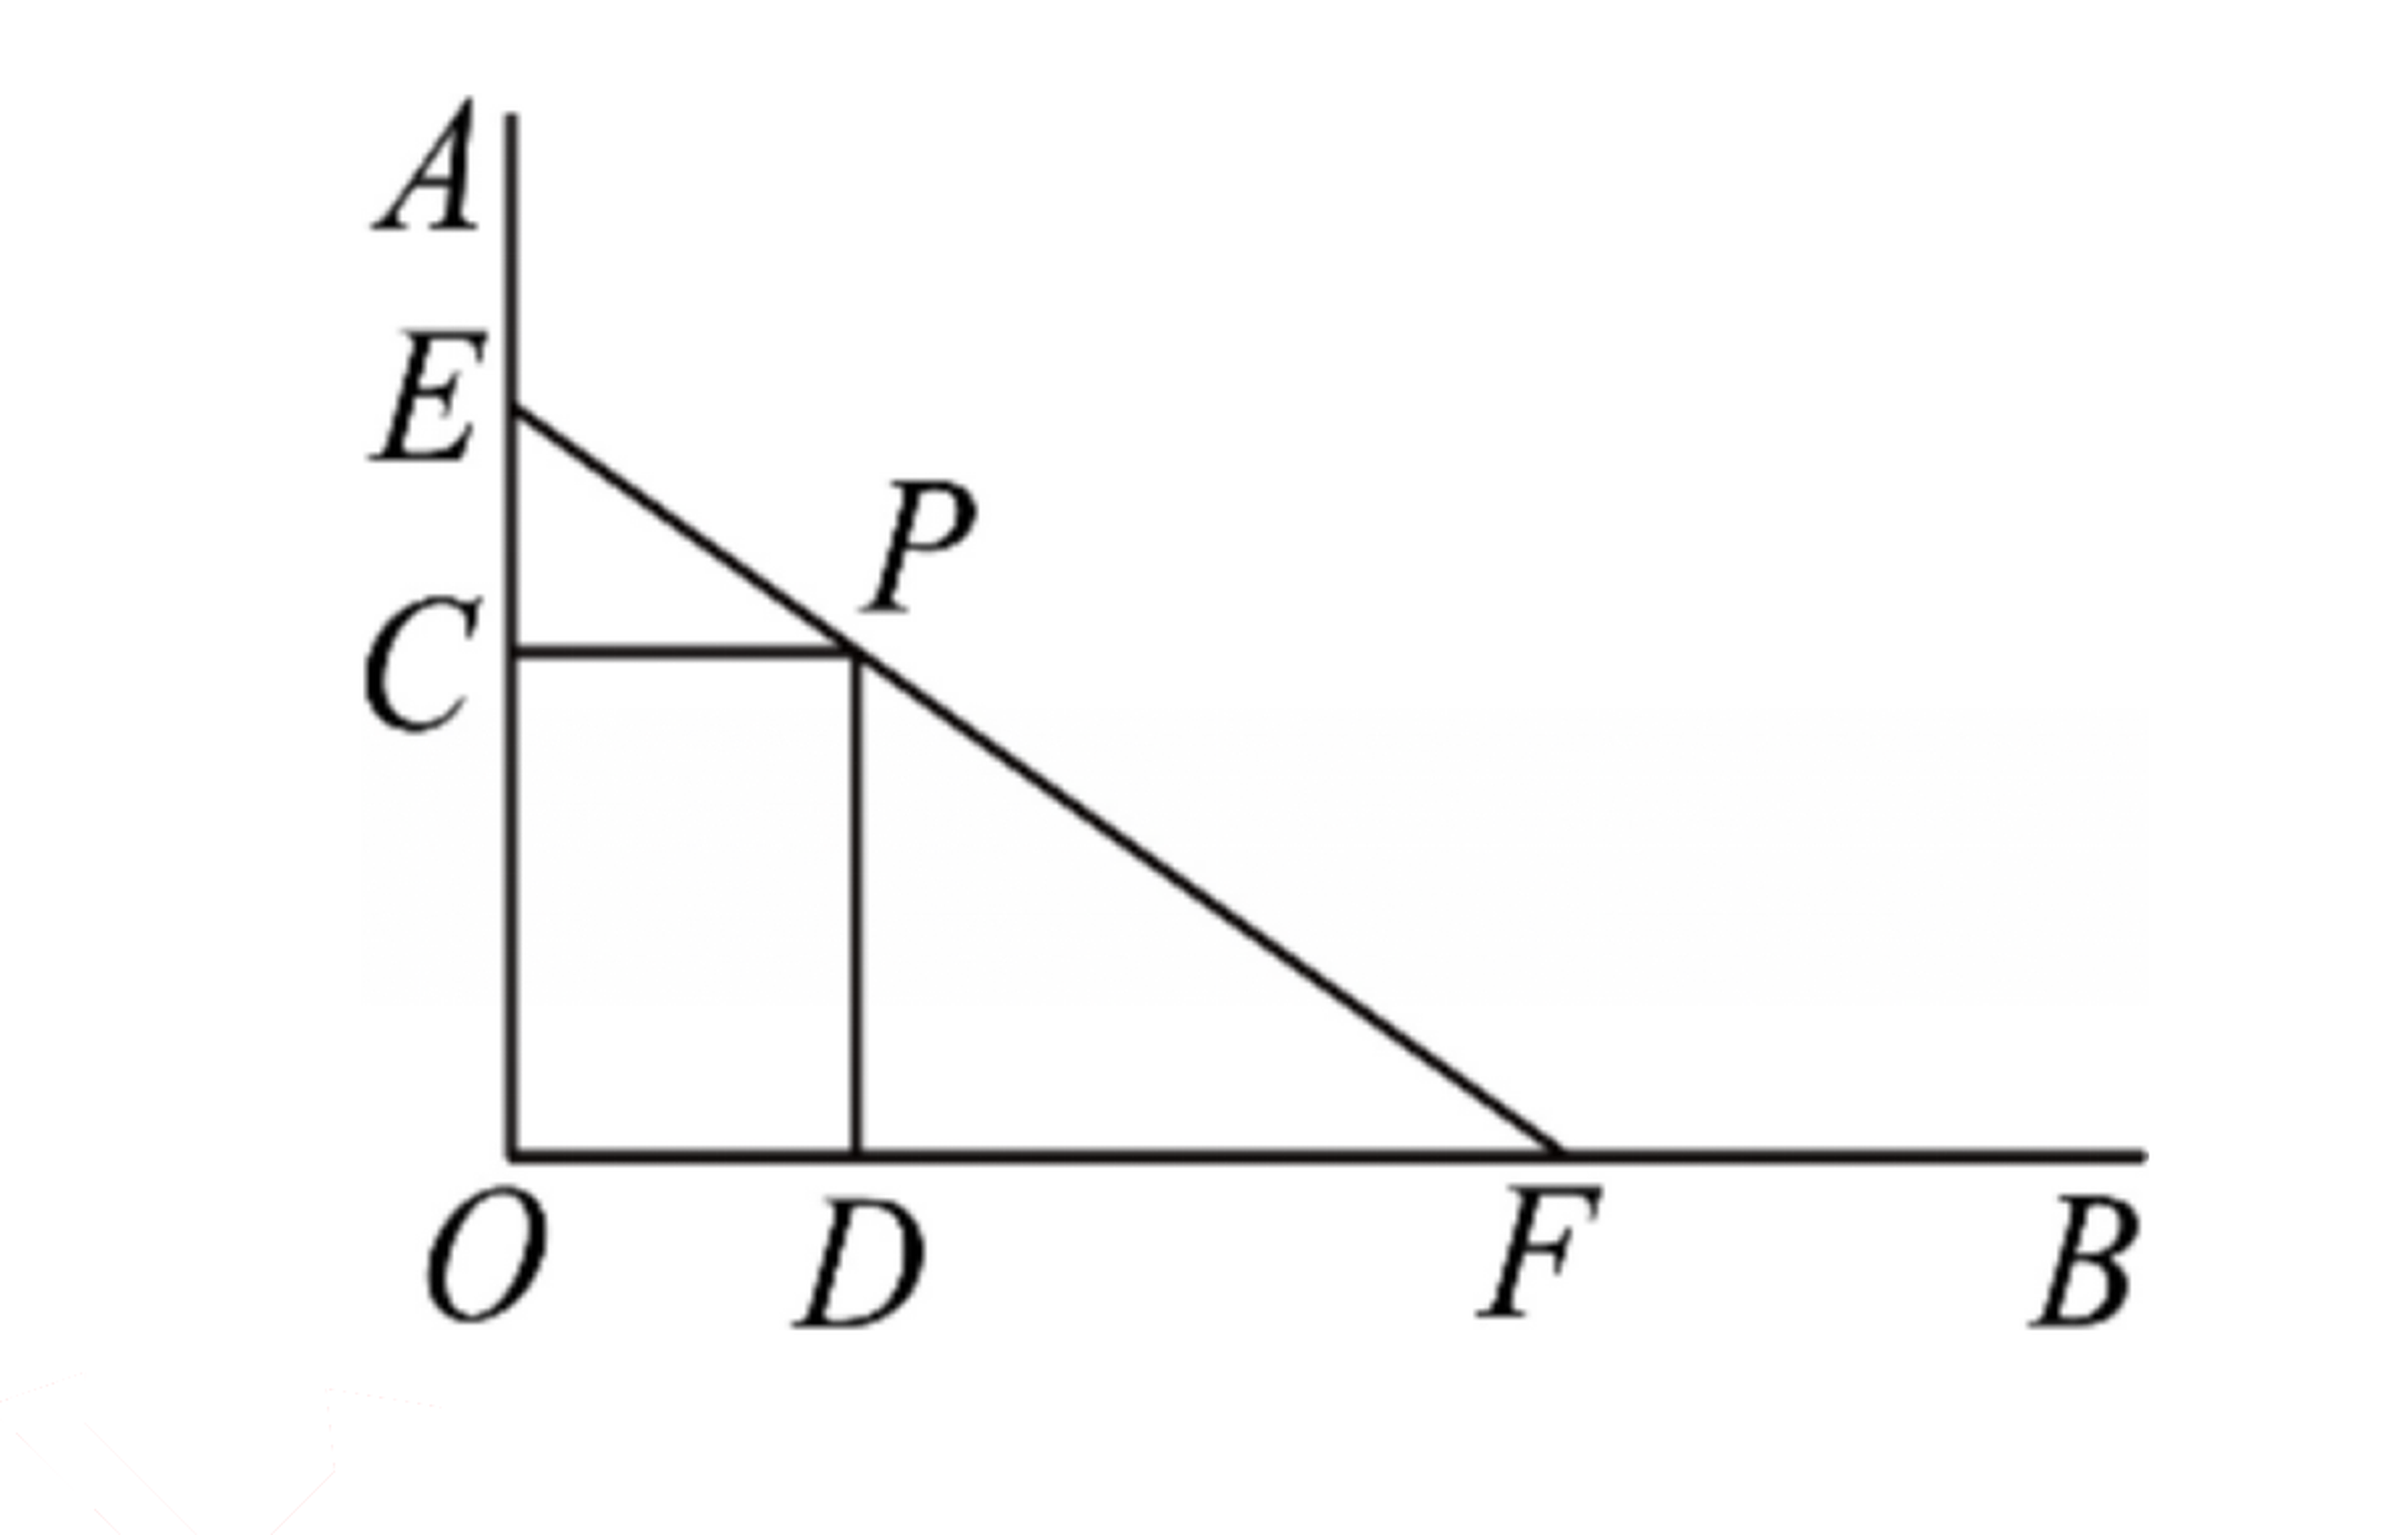
\includegraphics[width=0.32\textwidth]{figures/gao131_q19.png}
\end{center}

\ifanswer
\solbegin
\step{(1) 由题意得 $x\leq60$，}
\step{$\triangle PCE\sim\triangle FDP$，所以 $\dfrac{EC}{CP}=\dfrac{PD}{DF}$，即 $\dfrac{x}{25}=\dfrac{40}{DF}$，得 $DF=\dfrac{1000}{x}$m，}
\step{所以 $OF=OD+DF=\left(25+\dfrac{1000}{x}\right)$m，}
\step{所以 $25+\dfrac{1000}{x}\leq100$，解得 $x\geq\dfrac{40}{3}$；}
\step{综上，$\dfrac{40}{3}\leq x\leq60$；}
\step{(2) 由 $OE=OC+CE=(40+x)$m，}
\step{所以 $S=\dfrac12 OF\cdot OE=\dfrac12\left(25+\dfrac{1000}{x}\right)(40+x)$}
\step{$=\dfrac12\left(1000+25x+\dfrac{40000}{x}+1000\right)$m$^2$，}
\step{由基本不等式得 $S\geq\dfrac12\left(2000+2\sqrt{25x\cdot\dfrac{40000}{x}}\right)=2000$m$^2$，}
\step{当且仅当 $25x=\dfrac{40000}{x}$，即 $x=40$ 时取等号，}
\step{故 $EC=40$m 时，$S$ 取得最小值，为 $2000$m$^2$.}
\solend
\fi

\item 已知 $a\in\R$，函数 $y=ax^2+(3a+2)x+2a+3$.

(1) 当 $a=1$ 时，函数 $y=ax^2+(3a+2)x+2a+3$ 的图象与 $x$ 轴交于 $A(x_1,0)$，$B(x_2,0)$ 两点，求 $x_1^3+x_2^3$；

(2) 若关于 $x$ 的不等式 $ax^2+(3a+2)x+2a+3>2x$ 的解集为 $\R$，求实数 $a$ 的取值范围；

(3) 求关于 $x$ 的不等式 $y\geq1$ 的解集.

\ifanswer
\solbegin
\step{(1) 函数 $y=ax^2+(3a+2)x+2a+3$，当 $a=1$ 时，$y=x^2+5x+5$，}
\step{因为 $y=x^2+5x+5$ 的图象与 $x$ 轴交于 $A(x_1,0)$，$B(x_2,0)$ 两点，}
\step{即 $x^2+5x+5=0$ 的两个根为 $x_1$、$x_2$，}
\step{由根与系数的关系得 $x_1+x_2=-5$，$x_1x_2=5$，}
\step{所以 $x_1^2+x_2^2=(x_1+x_2)^2-2x_1x_2=25-10=15$，}
\step{所以 $x_1^3+x_2^3=(x_1+x_2)(x_1^2+x_2^2-x_1x_2)=-5\times(15-5)=-50$；}
\step{(2) 不等式 $ax^2+(3a+2)x+2a+3>2x$ 恒成立，得 $ax^2+3ax+2a+3>0$.}
\step{当 $a=0$ 时，$3>0$，恒成立，符合题意；}
\step{当 $a\neq0$ 时，若 $a<0$，二次函数 $ax^2+3ax+2a+3$ 开口向下，}
\step{一定存在小于零的部分，故不满足题意；}
\step{当 $a>0$ 时，若使 $ax^2+3ax+2a+3>0$ 恒成立，}
\step{只需 $\Delta=(3a)^2-4\times a\times(2a+3)=a^2-12a<0$，解得 $0<a<12$，}
\step{综上所述，$a$ 的取值范围为 $0\leq a<12$.}
\step{(3) 由 $y\geq1$，得 $ax^2+(3a+2)x+2a+3\geq1$，}
\step{即 $ax^2+(3a+2)x+2a+2\geq0$，即 $(ax+2a+2)(x+1)\geq0$，}
\step{当 $a=0$ 时，$2x+2\geq0$，解得 $x\geq-1$，}
\step{当 $a\neq0$ 时，}
\step{方程 $ax^2+(3a+2)x+2a+2=0$ 即为 $(x+1)(ax+2a+2)=0$，}
\step{解得 $x=-1$ 或 $x=-2-\dfrac2a$，令 $-1=-2-\dfrac2a$，即 $a=-2$，}
\step{当 $a>0$ 时，$-2-\dfrac2a<-1$，}
\step{不等式 $ax^2+(3a+2)x+2a+2\geq0$ 即为 $\left(x+\dfrac{2a+2}a\right)(x+1)\geq0$，}
\step{解得 $x\leq-2-\dfrac2a$ 或 $x\geq-1$；}
\step{当 $a<0$ 时，当 $-2-\dfrac2a<-1$，即 $a<-2$ 时，}
\step{不等式 $ax^2+(3a+2)x+2a+2\geq0$，即为 $\left(x+\dfrac{2a+2}a\right)(x+1)\leq0$，}
\step{解得 $-2-\dfrac2a\leq x\leq-1$；}
\step{当 $-2-\dfrac2a=-1$，即 $a=-2$，}
\step{不等式 $ax^2+(3a+2)x+2a+2\geq0$ 即为 $-2x^2-4x-2\geq0$，解得 $x=-1$，}
\step{当 $-2-\dfrac2a>-1$，即 $-2<a<0$ 时，}
\step{不等式 $ax^2+(3a+2)x+2a+2\geq0$ 即为 $\left(x+\dfrac{2a+2}a\right)(x+1)\leq0$，}
\step{解得 $-1\leq x\leq-2-\dfrac2a$，}
\step{综上所述，当 $a=0$ 时，解集为 $\{x\mid x\geq-1\}$；}
\step{当 $a>0$ 时，解集为 $\{x\mid x\leq-2-\dfrac2a$ 或 $x\geq-1\}$；}
\step{当 $a<-2$ 时，解集为 $\{x\mid -2-\dfrac2a\leq x\leq-1\}$；}
\step{当 $a=-2$ 时，解集为 $\{x\mid x=-1\}$；}
\step{当 $-2<a<0$ 时，解集为 $\{x\mid -1\leq x\leq-2-\dfrac2a\}$.}
\solend
\fi

\item 仔细阅读以下材料：【已知 $a$、$b\in(0,+\infty)$，$a+b=1$，求 $y=\dfrac1a+\dfrac2b$ 的最小值.

$y=\dfrac1a+\dfrac2b=\left(\dfrac1a+\dfrac2b\right)(a+b)=\dfrac ba+\dfrac{2a}b+3\geq3+2\sqrt2$，当且仅当 $\dfrac ba=\dfrac{2a}b$，即 $a=\sqrt2-1$，$b=2-\sqrt2$ 时取得等号，则 $y=\dfrac1a+\dfrac2b$ 的最小值为 $3+2\sqrt2$.

另 $y=\dfrac1a+\dfrac2b=\dfrac{a+b}a+\dfrac{2(a+b)}b=\dfrac ba+\dfrac{2a}b+3\geq3+2\sqrt2$，当且仅当 $\dfrac ba=\dfrac{2a}b$，即 $a=\sqrt2-1$，$b=2-\sqrt2$ 时取得等号，则 $y=\dfrac1a+\dfrac2b$ 的最小值为 $3+2\sqrt2$.】参考上述解法，求解下列问题.

(1) 若正实数 $x$、$y$ 满足 $x+y=1$，求 $\dfrac2x+\dfrac3y$ 的最小值；

(2) 已知 $x\in\left(0,\dfrac12\right)$，求 $t=\dfrac1x+\dfrac8{1-2x}$ 的最小值，并写出此时 $x$ 的值；

(3) 已知 $a$、$b\in(0,+\infty)$，$a+2b=1$，求 $p=\dfrac1{3a+4b}+\dfrac1{a+3b}$ 的最小值.

\ifanswer
\solbegin
\step{(1) 因为 $x>0,y>0$，且 $x+y=1$，}
\step{所以 $\dfrac2x+\dfrac3y=\left(\dfrac2x+\dfrac3y\right)(x+y)=2+\dfrac{2y}x+\dfrac{3x}y+3=5+\dfrac{2y}x+\dfrac{3x}y$，}
\step{由基本不等式得 $\dfrac{2y}x+\dfrac{3x}y\geq2\sqrt{\dfrac{2y}x\cdot\dfrac{3x}y}=2\sqrt6$，}
\step{当且仅当 $\dfrac{2y}x=\dfrac{3x}y$，即 $2y^2=3x^2$ 时，等号成立，}
\step{又因为 $x>0,y>0$ 且 $x+y=1$，此时 $x=\sqrt6-2,y=3-\sqrt6$，}
\step{所以 $\dfrac2x+\dfrac3y\geq5+2\sqrt6$，故 $\dfrac2x+\dfrac3y$ 的最小值为 $5+2\sqrt6$.}
\step{(2) 由 $0<x<\dfrac12$，则 $t=\dfrac1x+\dfrac8{1-2x}=\dfrac{2(1-2x+2x)}{2x}+\dfrac{8(1-2x+2x)}{1-2x}$}
\step{$=10+\dfrac{2\cdot(1-2x)}{2x}+\dfrac{8\cdot2x}{1-2x}\geq10+2\sqrt{\dfrac{2\cdot(1-2x)}{2x}\cdot\dfrac{8\cdot2x}{1-2x}}=18$，}
\step{当且仅当 $\dfrac{2\cdot(1-2x)}{2x}=\dfrac{8\cdot2x}{1-2x}$，即 $x=\dfrac16$ 时等号成立；}
\step{(3) 由 $a$、$b>0$，$a+2b=1$，则 $a=1-2b>0$，即 $0<b<\dfrac12$，}
\step{所以 $p=\dfrac1{3a+4b}+\dfrac1{a+3b}=\dfrac1{3a+6b-2b}+\dfrac1{a+2b+b}=\dfrac1{3-2b}+\dfrac1{1+b}$}
\step{$=\dfrac1{3-2b}+\dfrac2{2+2b}$，显然 $3-2b$、$2+2b>0$，}
\step{所以 $p=\dfrac15\cdot(3-2b+2+2b)\cdot\left(\dfrac1{3-2b}+\dfrac2{2+2b}\right)=\dfrac15\left[3+\dfrac{2+2b}{3-2b}+\dfrac{2(3-2b)}{2+2b}\right]$}
\step{$\geq\dfrac15\left[3+2\sqrt{\dfrac{2+2b}{3-2b}\cdot\dfrac{2(3-2b)}{2+2b}}\right]=\dfrac{3+2\sqrt2}5$，}
\step{当且仅当 $\dfrac{2+2b}{3-2b}=\dfrac{2(3-2b)}{2+2b}$，}
\step{即 $b=\dfrac{8-5\sqrt2}2$，$a=5\sqrt2-7$ 时等号成立.}
\solend
\fi

\end{enumerate}

\end{document}
"
% 紧凑版：xelatex "\def\iscompact{1}% 高一131_六十中学_期中.tex
%   —— 高一上数学"2026-2027 年六十中学高一上期中"（试卷版/答案版）
% 试卷版：xelatex 高一131_六十中学_期中.tex
% 答案版：xelatex "\def\isanswer{1}% 高一131_六十中学_期中.tex
%   —— 高一上数学"2026-2027 年六十中学高一上期中"（试卷版/答案版）
% 试卷版：xelatex 高一131_六十中学_期中.tex
% 答案版：xelatex "\def\isanswer{1}\input{高一131_六十中学_期中.tex}"
% 紧凑版：xelatex "\def\iscompact{1}\input{高一131_六十中学_期中.tex}"
%
% 原始材料：微信公众号"魔都数学加油站"文章，作者破晓，2026-11-13 18:18 发布；
% 连载"27学年高一131"，原文标题"27学年高一131——2026-2027年上海市六十中学高一上期中"；
% 原文链接：https://mp.weixin.qq.com/s/Nrbp3Uvt-sOGnOp4MEHemA。
% 正文为 11 张 PNG 页（01—05、09—11 为 2560x3620，06—08 为 4762x6735），
% 题目下印有【解析】或【答案】，为讲评版。题目、解析均据原图转录；
% 卷面粉红色水印"魔都数学加油站"及公众号页脚未录入。全卷仅第 19 题有 1 幅插图
% （矩形 OCPD 与小路 EF 的示意图），取 07.png 截图去水印。
%
% 卷首标题：原卷印作"2026-2027 年六十中学高一上期中"（公众号标题中的"上海市"
% 卷面标题行没有，本稿照卷面），年份区间按全稿惯例排 en dash；原卷未印副标题，
% 本卷为期中卷、跨集合与常用逻辑用语／不等式／函数三章，按题目内容标为
% "集合与常用逻辑用语、不等式、函数"（与 125／126／128／129 同期中卷口径相同）：
% 集合与逻辑见 Q3、Q4、Q7、Q13、Q17，不等式见 Q8、Q10、Q12、Q14、Q15、Q16、Q19、
% Q20、Q21，函数（指数／对数／幂函数、基本不等式应用）见 Q5、Q6、Q9、Q11、Q18、Q21。
%
% 题号体例：本卷共 19 题——一、填空题 3—12（10 题）、二、选择题 13—16（4 题）、
% 三、解答题 17—21（5 题）。三节分别 \setcounter{enumi}{2}／{12}／{16}。
%
% 与原卷的排版差异：
%   ① 原文从第 3 题起，本稿保留原题号（见上"题号体例"）；
%   ② 原卷每题下直接印【解析】／【答案】，本稿按全稿惯例置于答案版；第 3、4 题只印
%      【答案】，另提 \ans{}；第 13—16 题答案在解析末句"故选 …"，题干括号内留空、
%      不另提 \ans{}；其余各题印【解析】、无独立答案段；
%   ③ 原卷未印副标题，本稿按"知识模块"口径补出；
%   ④ 原卷填空横线按全稿惯例排为 \blankline[4.4em]；选择题括号排 \mbox{（\quad）}、
%      选项段前按惯例加 \keepwithprev；解答题不留作答区（原卷为讲评版，与 109—129 同）；
%   ⑤ 原卷数集排斜体 $R$／$N$，按全稿惯例改 \R／\N；绝对值排 \lvert…\rvert，
%      集合描述竖线排 \mid；不等号按全稿惯例排 \leqslant／\geqslant；
%   ⑥ 子题标号 (1)(2)(3) 原卷用半角括号，照录；圈数字 ①② 照录；
%   ⑦ 原卷第 19 题插图浮排在第 07 页题干右侧，本稿按体例就近置于题干"如图"之后
%      （居中 \includegraphics），图取原卷 07 页截图去水印；题前按惯例加
%      \needvspace{7cm} 守卫（照 高一120／127／129 成例），保证"题干 + 图"整块不被页边界切开；
%   ⑧ 原卷 Q9 题干跨 01—02 页、Q15 解析跨 03—04 页、Q16 材料跨 04—05 页、
%      Q17 题干跨 05—06 页、Q20 解析跨 08—09 页、Q21 解析跨 09—11 页，
%      本稿按题合并连续排版；末页第 11 页为 Q21 (3) 解析的续尾，按实际印刷行单列。
%   ⑨ 第 16 题材料英文括注原卷印作 (Cauchy – SchwarzInequality)（长横、Schwarz 与
%      Inequality 斜体连排无空格），本稿按全稿英文专名惯例排 \emph{(Cauchy-Schwarz Inequality)}；
%      第 15 题解析 B、D 两行原卷各印一步含 \lg m 的换底繁分数（2026-11-13 回原图核对补回，
%      本稿初转曾顺手去重跳过该步）。
%
% 判别式字形：第 20 题 (2) 解析 $\Delta=(3a)^2-4\times a\times(2a+3)=a^2-12a<0$
%   原卷排三角形（等腰、高；回 08.png 放大核对），照录 \Delta；全卷判别式仅此一处
%   （\triangle 另作第 19 题「$\triangle PCE\sim\triangle FDP$」的几何三角形记号）。
%
% 子集符号：第 17 题 (2) 解析 $P\subseteq Q$ 印带下划线，照录 \subseteq；
%   全卷未出现单线 \subset。
%
% 原卷存疑照录：
%   第 11 题解析末两式作 $\dfrac{2+m+\frac1n}{2n+2}=\dfrac{2n+mn+1}{2n+2}$，而第三式
%     分母 $\log_3 9+\log_3 2+\log_3 2=2+\frac2n$，与前一分母 $2n+2$ 不等，照录；
%   第 16 题材料 ①"对于所有实数 $x$ 和 $y$，有 $(a^2+b^2)(c^2+d^2)\geq(ac+bd)^2$"
%     句首用 $x$、$y$ 而式中用 $a$、$b$、$c$、$d$，照录；
%   第 20 题题干 (2) 作"解集为 $\R$"、解析 (2) 作"恒成立"，措辞不同，照录；
%   第 21 题材料把同一道题用两种解法连印两遍（"另 $y=\frac1a+\frac2b=\dots$"），照录；
%   第 21 题 (3) 解析末句"即 $b=\frac{8-5\sqrt2}{2}$，$a=5\sqrt2-7$ 时等号成立"
%     未另写"故最小值为 $\frac{3+2\sqrt2}{5}$"，照录；
%   第 12 题解析"所以 $e^a+e^b>e^c, a+b>c$"、第 8 题解析"$a>0$，$b>0$"、
%     第 18 题 (2)"$4x^2-4x+1<x^2+4x+4$，解得 $-\frac13<x<3$"等处数学式内
%     半角逗号，照录；
%   第 15 题解析用 $\lg$ 记常用对数（$\lg m$、$\lg 3$、$\lg 5$、$\lg 15$），照录。
%
% 行数复核：逐题数 \step 条数，合计 119 条（Q3：0；Q4：0；Q5：1；Q6：1；Q7：2；
% Q8：2；Q9：1；Q10：1；Q11：2；Q12：6；Q13：2；Q14：3；Q15：14；Q16：10；
% Q17：4；Q18：8；Q19：11；Q20：35；Q21：16），与原卷印刷行逐题相等
% （cases 块作一个印刷行计）。第 3、4 题只印【答案】，提 \ans{}，不计入 \step 账；
% 四道选择题答案均在解析末句，括号内留空、不另提 \ans{}。
%
\documentclass[a4paper,11pt]{article}
\usepackage{common}

\begin{document}

\examtitlest[3]{2026--2027 年六十中学高一上期中}{集合与常用逻辑用语、不等式、函数}

\bigsec{一、填空题}

\begin{enumerate}
\setcounter{enumi}{2}

\item 已知集合 $A=(0,4),B=[2,5]$，则 $A\cup B=$\blankline[4.4em].

\ifanswer
\ans{$(0,5]$}
\fi

\item 陈述句“$x=2$ 或 $y=3$”的否定形式为\blankline[4.4em].

\ifanswer
\ans{$x\neq2$ 且 $y\neq3$}
\fi

\item 函数 $y=a^{x-2}+15(a>0$ 且 $a\neq1)$ 的图象恒过定点的坐标为\blankline[4.4em].

\ifanswer
\solbegin
\step{函数 $y=a^{x-2}+15$ 的图象恒过定点 $A(2,16)$.}
\solend
\fi

\item 用有理数指数幂的形式来化简：$\dfrac{\sqrt{a\cdot\sqrt[3]{a^4}}}{\left(a^{\frac13}\right)^2}=$\blankline[4.4em].

\ifanswer
\solbegin
\step{原式 $=\dfrac{\sqrt{a\cdot a^{\frac43}}}{a^{\frac23}}=\dfrac{\sqrt{a^{\frac73}}}{a^{\frac23}}=\dfrac{a^{\frac76}}{a^{\frac23}}=a^{\frac76-\frac23}=a^{\frac12}(a>0)$.}
\solend
\fi

\item 已知集合 $A=\left\{x\mid \dfrac6{6-x}\in\N\text{ 且 }x\in\N\right\}$，则用列举法表示集合 $A=$\blankline[4.4em].

\ifanswer
\solbegin
\step{当 $x=0$ 时，$\dfrac6{6-0}=1\in\N$，当 $x=3$ 时，$\dfrac6{6-3}=2\in\N$，}
\step{当 $x=4$ 时，$\dfrac6{6-4}=3\in\N$，当 $x=5$ 时，$\dfrac6{6-5}=6\in\N$，故 $A=\{0,3,4,5\}$.}
\solend
\fi

\item 已知 $a>0$，$b>0$，且 $ab=\dfrac12$，则 $\dfrac1a+\dfrac8b$ 的最小值是\blankline[4.4em].

\ifanswer
\solbegin
\step{$a>0$，$b>0$，且 $ab=\dfrac12$，则 $\dfrac1a+\dfrac8b\geq2\sqrt{\dfrac8{ab}}=8$，}
\step{当且仅当 $\dfrac1a=\dfrac8b$，即 $a=\dfrac14,b=2$ 时取等号，故最小值为 $8$.}
\solend
\fi

\item 心理学家有时用函数 $L(t)=A(1-e^{-kt})$ 测定在时间 $t$（单位：$min$）内能够记忆的量 $L$，其中 $A$ 表示需要记忆的量，$k$ 表示记忆率. 假设一个学生需要记忆的量为 $200$ 个单词，此时 $L$ 表示在时间 $t$ 内该生能够记忆的单词个数. 已知该生在 $5min$ 内能够记忆 $20$ 个单词，则 $k$ 的值约为\blankline[4.4em]（结果保留四位小数）.

\ifanswer
\solbegin
\step{由题意得 $200(1-e^{-5k})=20$，所以 $e^{-5k}=0.9$，解得 $k\approx0.0211$.}
\solend
\fi

\item 设 $x\in\R$，方程 $\lvert 3x-2\rvert+\lvert 1-x\rvert=\lvert 2x-1\rvert$ 的解集是\blankline[4.4em].

\ifanswer
\solbegin
\step{由三角不等式得 $(3x-2)(1-x)\geq0$，故解集是 $\left[\dfrac23,1\right]$.}
\solend
\fi

\item 已知 $3^m=5$，$n=\log_2 3$，则 $\log_{36}90$ 可用 $m$、$n$ 表示为\blankline[4.4em].

\ifanswer
\solbegin
\step{由 $3^m=5$，又 $n=\log_2 3$，得 $m=\log_3 5$，$\log_3 2=\dfrac{\log_2 2}{\log_2 3}=\dfrac1n$，}
\step{所以 $\log_{36}90=\dfrac{\log_3 90}{\log_3 36}=\dfrac{\log_3 9+\log_3 2+\log_3 5}{\log_3 9+\log_3 2+\log_3 2}=\dfrac{2+m+\frac1n}{2n+2}=\dfrac{2n+mn+1}{2n+2}$.}
\solend
\fi

\item 若定义域为 $I=(0,m]$ 的函数 $f(x)=e^x$ 满足：对任意能构成三角形三边长的实数 $a$、$b$、$c\in I$，均有 $f(a)$、$f(b)$、$f(c)$ 也能构成三角形三边长，则 $m$ 的最大值为\blankline[4.4em].

\ifanswer
\solbegin
\step{$f(x)=e^x$ 在 $I=(0,m]$ 上严格增，所以 $f(x)\in(1,e^m]$，不妨设 $0<a\leq b\leq c$，}
\step{因为对任意能构成三角形三边长的实数 $a,b,c\in I$，均有 $f(a)$，$f(b)$，$f(c)$}
\step{也能构成三角形三边长，所以 $e^a+e^b>e^c, a+b>c$，}
\step{因为 $e^a+e^b\geq2\sqrt{e^ae^b}=2\sqrt{e^{a+b}}>e^c$，所以 $4e^{a+b}>e^{2c}$，}
\step{因为对任意 $a,b,c\in I$ 都成立，所以 $4e^c\geq e^{2c}$，所以 $e^c\leq4$，所以 $c\leq\ln4$，}
\step{所以 $m\leq\ln4$，所以 $m$ 的最大值为 $\ln4$.}
\solend
\fi

\end{enumerate}

\bigsec{二、选择题}

\begin{enumerate}
\setcounter{enumi}{12}

\item 已知 $m,n$ 是非零自然数，命题 $\alpha:mn$ 是奇数，命题 $\beta:m$ 或 $n$ 是奇数，则 $\alpha$ 是 $\beta$ 的\mbox{（\quad）}

\keepwithprev
A. 充分非必要条件\qquad\qquad B. 必要非充分条件

C. 充要条件\qquad\qquad D. 既非充分又非必要条件

\ifanswer
\solbegin
\step{$mn$ 是奇数 $\Leftrightarrow$ $m$、$n$ 都是奇数，所以 $\alpha$ 能推出 $\beta$，充分性成立，}
\step{但 $\beta$ 推不出 $\alpha$，必要性不成立，所以 $\alpha$ 是 $\beta$ 的充分非必要条件. 故选 $A$.}
\solend
\fi

\item 关于 $x$ 的不等式 $x^2-mx+n+5\leq0$ 的解集是 $[1,8]$，那么 $\log_m n=$\mbox{（\quad）}

\keepwithprev
A. $\dfrac13$\qquad\qquad B. $-3$\qquad\qquad C. $-2$\qquad\qquad D. $\dfrac12$

\ifanswer
\solbegin
\step{由题意得 $x^2-mx+n+5=0$ 的解为 $1$，$8$，}
\step{由根与系数的关系得 $\begin{cases}1+8=m\\1\times8=n+5\end{cases}$，解得 $m=9$，$n=3$，}
\step{所以 $\log_m n=\log_9 3=\dfrac12\log_3 3=\dfrac12$. 故选 $D$.}
\solend
\fi

\item 已知正实数 $x$、$y$、$z$ 满足 $3^x=5^y=15^z$，则下列说法中不正确的是\mbox{（\quad）}

\keepwithprev
A. $\dfrac1x+\dfrac1y=\dfrac1z$\qquad\qquad B. $x+y>2z$\qquad\qquad C. $3x>5y>15z$\qquad\qquad D. $x\cdot y>4z^2$

\ifanswer
\solbegin
\step{已知正实数 $x$、$y$、$z$，则设 $3^x=5^y=15^z=m>1$，}
\step{所以 $x=\log_3 m$，$y=\log_5 m$，$z=\log_{15} m$，}
\step{对于 $A$，$\dfrac1x+\dfrac1y=\dfrac1{\log_3 m}+\dfrac1{\log_5 m}=\log_m 3+\log_m 5=\log_m 15=\dfrac1z$，故 $A$ 正确；}
\step{对于 $B$，因为 $\dfrac{x+y}{z}=\dfrac{x}{z}+\dfrac{y}{z}=\dfrac{\log_3 m}{\log_{15} m}+\dfrac{\log_5 m}{\log_{15} m}=\dfrac{\dfrac{\lg m}{\lg3}}{\dfrac{\lg m}{\lg15}}+\dfrac{\dfrac{\lg m}{\lg5}}{\dfrac{\lg m}{\lg15}}=\dfrac{\lg15}{\lg3}+\dfrac{\lg15}{\lg5}$，}
\step{$=\dfrac{\lg3+\lg5}{\lg3}+\dfrac{\lg3+\lg5}{\lg5}=2+\dfrac{\lg5}{\lg3}+\dfrac{\lg3}{\lg5}=2+\log_3 5+\log_5 3$，}
\step{又 $\log_3 5>0$，$\log_5 3>0$，所以 $2+\log_3 5+\log_5 3>2$，}
\step{所以 $\dfrac{x+y}{z}>2$，即 $x+y>2z$，故 $B$ 正确；}
\step{对于 $C$，因为 $\dfrac5x=5\log_m 3=\log_m 243$，$\dfrac3y=3\log_m 5=\log_m 125$，}
\step{所以 $\dfrac5x>\dfrac3y$，即 $3x<5y$，故 $C$ 错误；}
\step{对于 $D$，$\dfrac{xy}{z^2}=\dfrac{x}{z}\cdot\dfrac{y}{z}=\dfrac{\log_3 m}{\log_{15} m}\cdot\dfrac{\log_5 m}{\log_{15} m}=\dfrac{\dfrac{\lg m}{\lg3}}{\dfrac{\lg m}{\lg15}}\cdot\dfrac{\dfrac{\lg m}{\lg5}}{\dfrac{\lg m}{\lg15}}=\dfrac{\lg15}{\lg3}\cdot\dfrac{\lg15}{\lg5}$}
\step{$=\dfrac{\lg3+\lg5}{\lg3}\cdot\dfrac{\lg3+\lg5}{\lg5}=\left(1+\dfrac{\lg5}{\lg3}\right)\left(1+\dfrac{\lg3}{\lg5}\right)=2+\dfrac{\lg5}{\lg3}+\dfrac{\lg3}{\lg5}$}
\step{$\geq2+2\sqrt{\dfrac{\lg5}{\lg3}\cdot\dfrac{\lg3}{\lg5}}=2+2=4$，又 $\lg3\neq\lg5$，故等号不成立，}
\step{所以 $\dfrac{xy}{z^2}>4$，即 $xy>4z^2$，故 $D$ 正确.}
\step{故选 $C$.}
\solend
\fi

\item 柯西不等式 \emph{(Cauchy-Schwarz Inequality)} 是一种在数学和物理学中广泛使用的不等式，它是由法国数学家奥古斯丁$\cdot$路易$\cdot$柯西提出的，柯西不等式可以用于证明其他不等式，也可以用于解决一些数学问题. 以下是柯西不等式的原始形式：

①对于所有实数 $x$ 和 $y$，有 $(a^2+b^2)(c^2+d^2)\geq(ac+bd)^2$.

②等式条件：当且仅当 $ad-bc=0$ 时，等号成立.

例：已知 $x+2y=2$，由柯西不等式 $(x^2+y^2)(1^2+2^2)\geq(x+2y)^2$，可得 $(x^2+y^2)_{min}=\dfrac45$.

现给出以下两个命题：

①若 $a^2+b^2=1$，则 $2a+3b$ 的最大值为 $\sqrt{13}$；

②若 $1<a<3$，则 $\sqrt{a-1}+\sqrt{6-2a}$ 的最大值为 $\sqrt6$；

则运用柯西不等式，判断以下正确的选项有\mbox{（\quad）}

\keepwithprev
A. ①为真命题；②为真命题\qquad\qquad B. ①为真命题；②为假命题

C. ①为假命题；②为真命题\qquad\qquad D. ①为假命题；②为假命题

\ifanswer
\solbegin
\step{由柯西不等式得 $(a^2+b^2)(2^2+3^2)\geq(2a+3b)^2$.}
\step{因为 $a^2+b^2=1$，所以 $(2^2+3^2)\geq(2a+3b)^2$，即 $13\geq(2a+3b)^2$，}
\step{所以 $-\sqrt{13}\leq2a+3b\leq\sqrt{13}$，则 $(2a+3b)_{max}=\sqrt{13}$，}
\step{当且仅当 $3a=2b$ 时取等号，故①正确.}
\step{令 $x=\sqrt{a-1}$，$y=\sqrt{3-a}$，则 $x^2+y^2=a-1+3-a=2$，}
\step{由柯西不等式得 $(\sqrt{a-1}+\sqrt{6-2a})^2=(\sqrt{a-1}+\sqrt2\cdot\sqrt{3-a})^2=(x+\sqrt2 y)^2$}
\step{$\leq[1^2+(\sqrt2)^2](x^2+y^2)$，}
\step{因为 $x^2+y^2=2$，所以 $(\sqrt{a-1}+\sqrt{6-2a})^2\leq6$，}
\step{当且仅当 $\sqrt{3-a}=\sqrt2\sqrt{a-1}$ 取等号，所以 $\sqrt{a-1}+\sqrt{6-2a}\leq\sqrt6$，故②正确.}
\step{故选 $A$.}
\solend
\fi

\end{enumerate}

\bigsec{三、解答题}

\begin{enumerate}
\setcounter{enumi}{16}

\item 已知集合 $P=\left\{x\mid \dfrac{3x-1}{x+2}<1\right\}$，集合 $Q=\{x\mid\lvert x-a\rvert\leq2\}$.

(1) 求集合 $P$；

(2) 若“$x\in P$”是“$x\in Q$”的充分非必要条件，求实数 $a$ 的取值范围.

\ifanswer
\solbegin
\step{(1) 集合 $P=\left\{x\mid \dfrac{3x-1}{x+2}<1\right\}$，得 $\dfrac{2x-3}{x+2}<0$，解得 $P=\left(-2,\dfrac32\right)$.}
\step{(2) 集合 $Q=\{x\mid\lvert x-a\rvert\leq2\}=\{x\mid a-2\leq x\leq2+a\}$，}
\step{由“$x\in P$”是“$x\in Q$”的充分非必要条件，得 $P\subseteq Q$，}
\step{得 $\begin{cases}-2\geq a-2\\\dfrac32\leq2+a\\a-2<2+a\end{cases}$，解得 $a\in\left[-\dfrac12,0\right]$.}
\solend
\fi

\item 已知幂函数 $f(x)=(m^2-4m+4)\cdot x^{2m-4}$ 在 $(-\infty,0)$ 上是严格减函数.

(1) 求函数 $y=f(x)$ 的解析式；

(2) 若 $f(1-2x)<f(x+2)$，求 $x$ 的取值范围.

\ifanswer
\solbegin
\step{(1) 由幂函数的定义得 $m^2-4m+4=1$，解得 $m=1$ 或 $3$，}
\step{当 $m=1$ 时，$f(x)=x^{-2}=\dfrac1{x^2}$，在 $(-\infty,0)$ 上严格增，不符合题意，}
\step{当 $m=3$ 时，$f(x)=x^2$，在 $(-\infty,0)$ 上严格减，符合题意，}
\step{所以 $f(x)=x^2$；}
\step{(2) 由函数 $f(x)=x^2$ 图象关于 $y$ 轴对称，且在 $[0,+\infty)$ 上严格增，}
\step{则 $f(1-2x)<f(x+2)$ 可化为 $\lvert1-2x\rvert<\lvert x+2\rvert$，}
\step{平方得 $4x^2-4x+1<x^2+4x+4$，解得 $-\dfrac13<x<3$，}
\step{所以 $x$ 的取值范围是 $\left(-\dfrac13,3\right)$.}
\solend
\fi

% 第 19 题是"题干 + 图"约 7cm 的一整块，守卫放在 \item 之前（放 \item 之后会失效）
\needvspace{7cm}
\item 如图，$OA$、$OB$ 是两条长度足够长的互相垂直的笔直小路，矩形 $OCPD$ 的顶点 $C$，$D$ 分别在 $OA$、$OB$ 上，且该矩形区域内种满了荷花. 为了让观赏者有更好的观赏体验，现计划经过点 $P$ 修一条小路 $EF$，其中点 $E$ 在小路 $OA$ 上，点 $F$ 在小路 $OB$ 上，并在 $\triangle OEF$ 区域内种满荷花. 已知 $OD=25m$，$OC=40m$，且小路 $EF$ 要完全位于一个以 $O$ 为顶点的，边长为 $100$ m 的正方形内部（包括边界）. 记 $\triangle OEF$ 的面积为 $S$m$^2$.

(1) 设 $EC=x\cdot m$，试用 $x$ 表示 $OF$，并求 $x$ 的取值范围.

(2) 当 $EC$ 的长度为多少时，$S$ 取得最小值？最小值是多少？

\begin{center}
% 图取原卷 07.png 截图去粉色水印，2.8× LANCZOS 放大
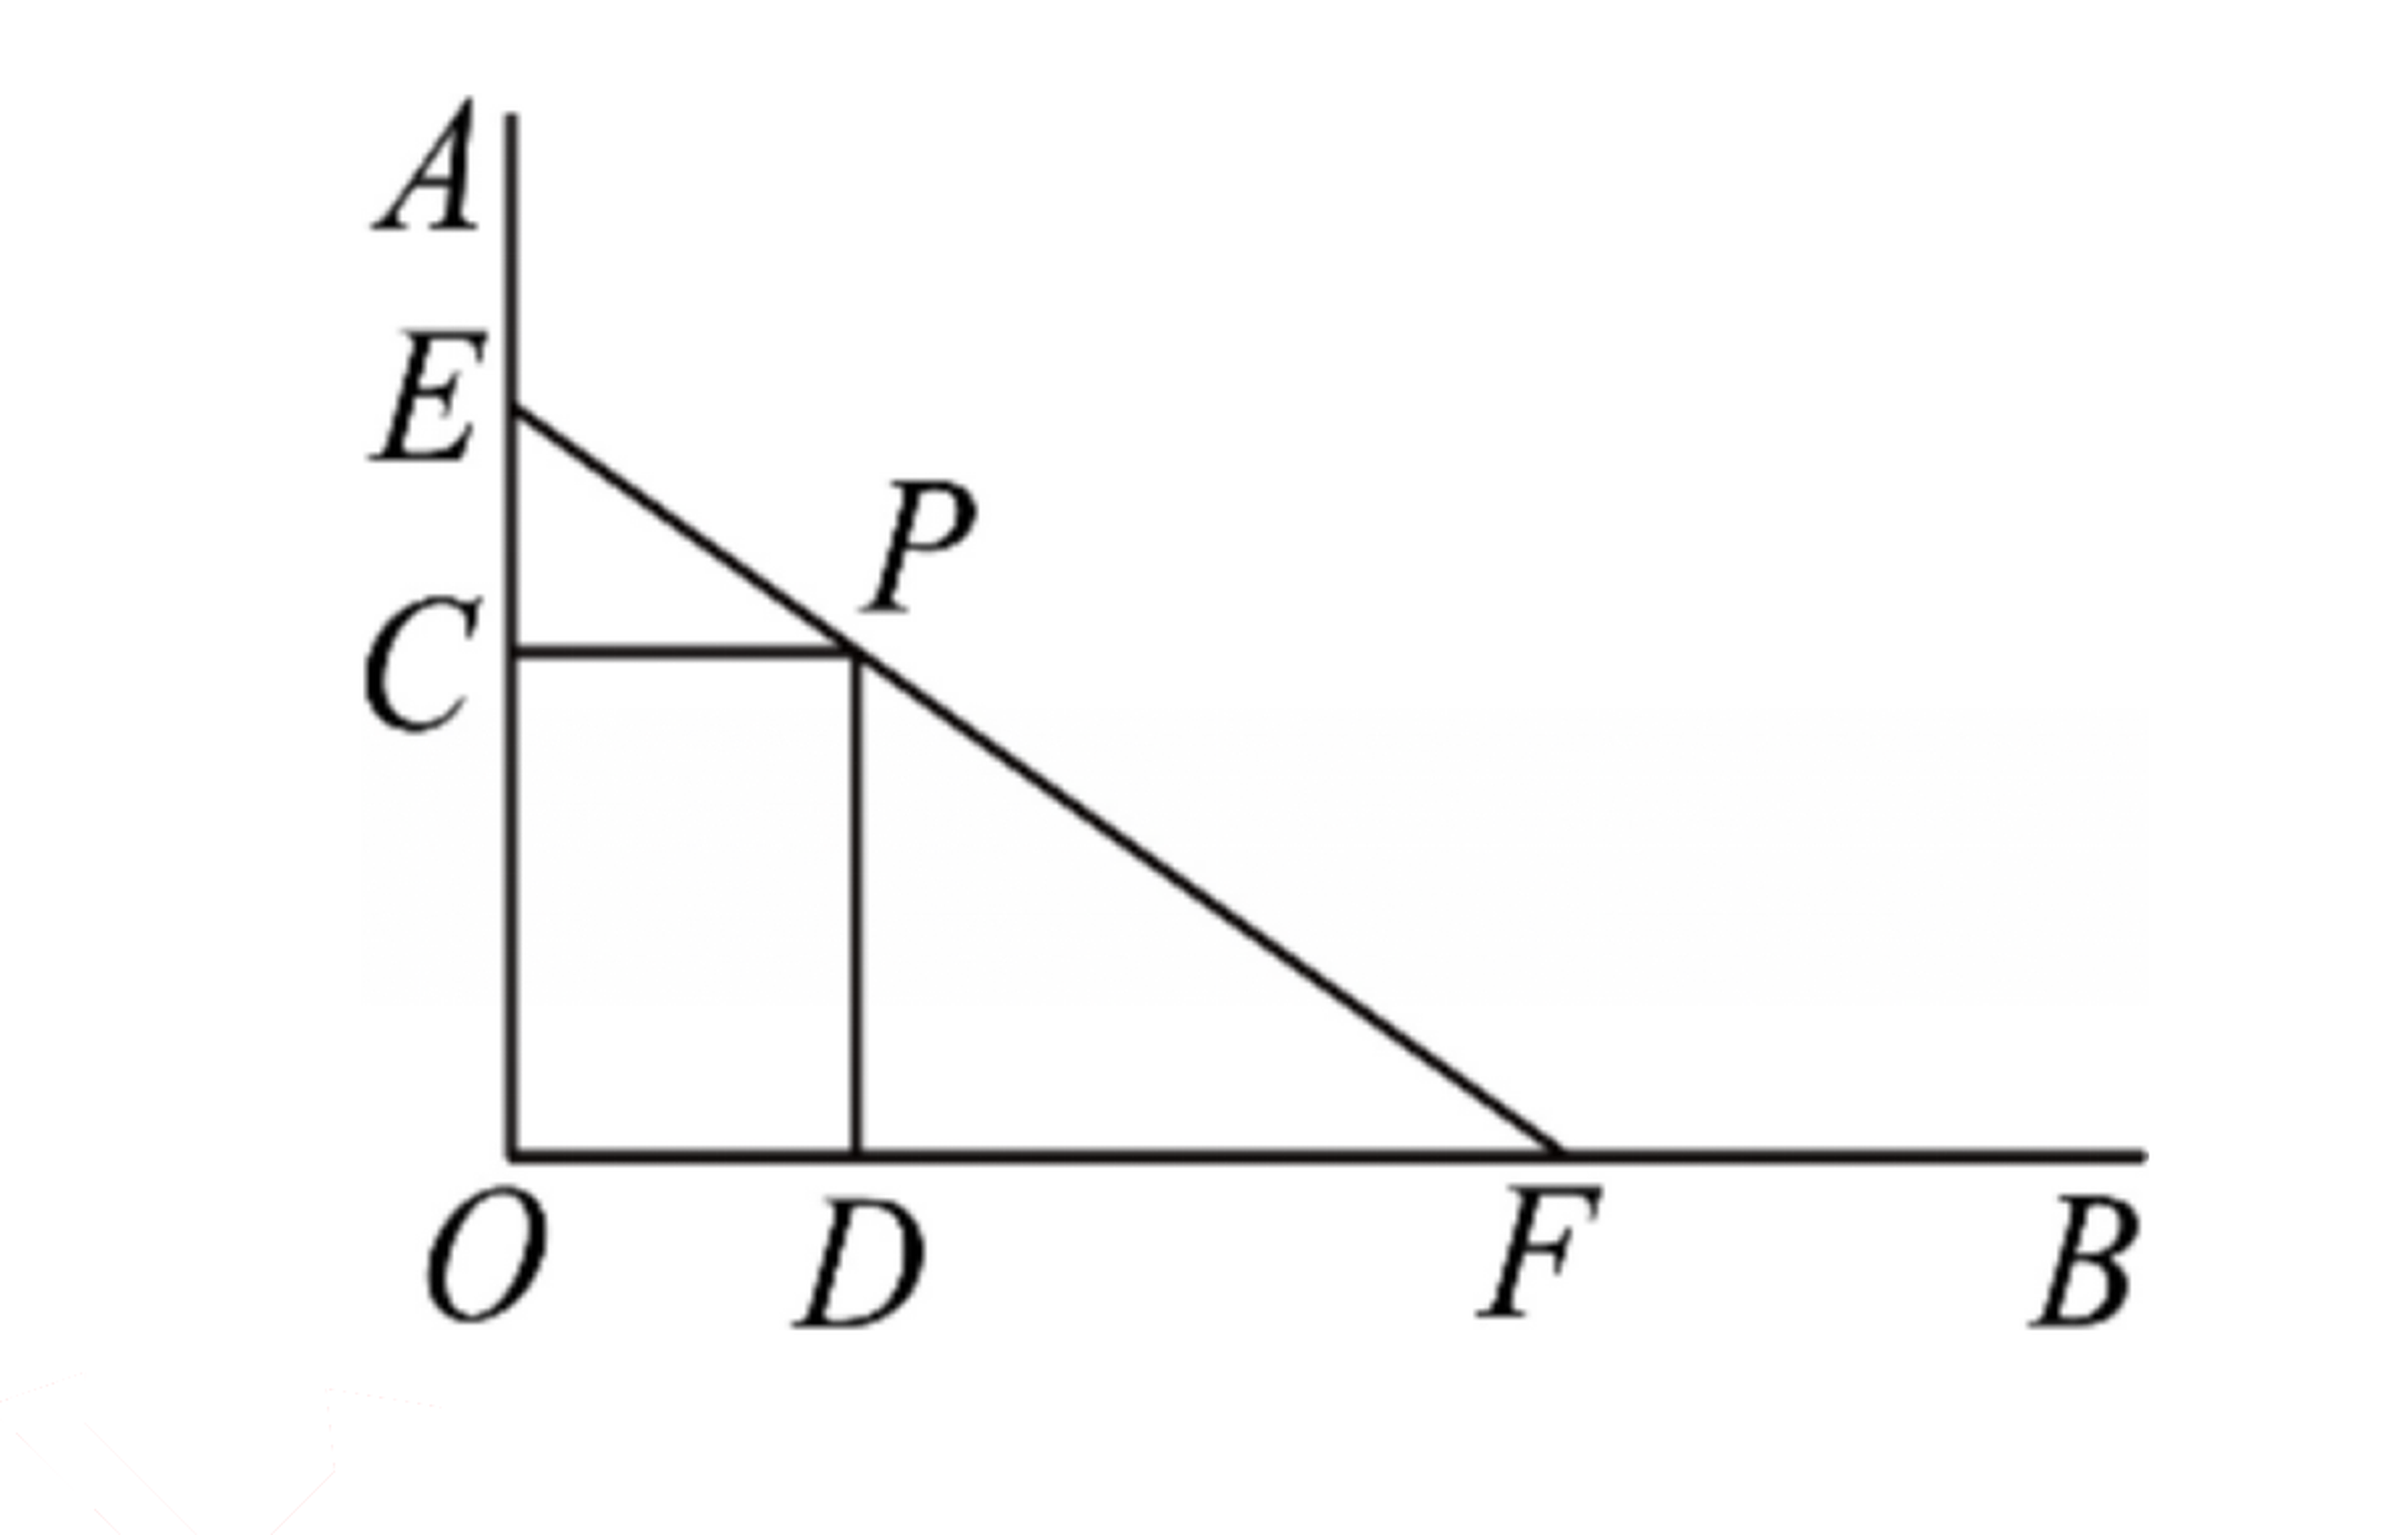
\includegraphics[width=0.32\textwidth]{figures/gao131_q19.png}
\end{center}

\ifanswer
\solbegin
\step{(1) 由题意得 $x\leq60$，}
\step{$\triangle PCE\sim\triangle FDP$，所以 $\dfrac{EC}{CP}=\dfrac{PD}{DF}$，即 $\dfrac{x}{25}=\dfrac{40}{DF}$，得 $DF=\dfrac{1000}{x}$m，}
\step{所以 $OF=OD+DF=\left(25+\dfrac{1000}{x}\right)$m，}
\step{所以 $25+\dfrac{1000}{x}\leq100$，解得 $x\geq\dfrac{40}{3}$；}
\step{综上，$\dfrac{40}{3}\leq x\leq60$；}
\step{(2) 由 $OE=OC+CE=(40+x)$m，}
\step{所以 $S=\dfrac12 OF\cdot OE=\dfrac12\left(25+\dfrac{1000}{x}\right)(40+x)$}
\step{$=\dfrac12\left(1000+25x+\dfrac{40000}{x}+1000\right)$m$^2$，}
\step{由基本不等式得 $S\geq\dfrac12\left(2000+2\sqrt{25x\cdot\dfrac{40000}{x}}\right)=2000$m$^2$，}
\step{当且仅当 $25x=\dfrac{40000}{x}$，即 $x=40$ 时取等号，}
\step{故 $EC=40$m 时，$S$ 取得最小值，为 $2000$m$^2$.}
\solend
\fi

\item 已知 $a\in\R$，函数 $y=ax^2+(3a+2)x+2a+3$.

(1) 当 $a=1$ 时，函数 $y=ax^2+(3a+2)x+2a+3$ 的图象与 $x$ 轴交于 $A(x_1,0)$，$B(x_2,0)$ 两点，求 $x_1^3+x_2^3$；

(2) 若关于 $x$ 的不等式 $ax^2+(3a+2)x+2a+3>2x$ 的解集为 $\R$，求实数 $a$ 的取值范围；

(3) 求关于 $x$ 的不等式 $y\geq1$ 的解集.

\ifanswer
\solbegin
\step{(1) 函数 $y=ax^2+(3a+2)x+2a+3$，当 $a=1$ 时，$y=x^2+5x+5$，}
\step{因为 $y=x^2+5x+5$ 的图象与 $x$ 轴交于 $A(x_1,0)$，$B(x_2,0)$ 两点，}
\step{即 $x^2+5x+5=0$ 的两个根为 $x_1$、$x_2$，}
\step{由根与系数的关系得 $x_1+x_2=-5$，$x_1x_2=5$，}
\step{所以 $x_1^2+x_2^2=(x_1+x_2)^2-2x_1x_2=25-10=15$，}
\step{所以 $x_1^3+x_2^3=(x_1+x_2)(x_1^2+x_2^2-x_1x_2)=-5\times(15-5)=-50$；}
\step{(2) 不等式 $ax^2+(3a+2)x+2a+3>2x$ 恒成立，得 $ax^2+3ax+2a+3>0$.}
\step{当 $a=0$ 时，$3>0$，恒成立，符合题意；}
\step{当 $a\neq0$ 时，若 $a<0$，二次函数 $ax^2+3ax+2a+3$ 开口向下，}
\step{一定存在小于零的部分，故不满足题意；}
\step{当 $a>0$ 时，若使 $ax^2+3ax+2a+3>0$ 恒成立，}
\step{只需 $\Delta=(3a)^2-4\times a\times(2a+3)=a^2-12a<0$，解得 $0<a<12$，}
\step{综上所述，$a$ 的取值范围为 $0\leq a<12$.}
\step{(3) 由 $y\geq1$，得 $ax^2+(3a+2)x+2a+3\geq1$，}
\step{即 $ax^2+(3a+2)x+2a+2\geq0$，即 $(ax+2a+2)(x+1)\geq0$，}
\step{当 $a=0$ 时，$2x+2\geq0$，解得 $x\geq-1$，}
\step{当 $a\neq0$ 时，}
\step{方程 $ax^2+(3a+2)x+2a+2=0$ 即为 $(x+1)(ax+2a+2)=0$，}
\step{解得 $x=-1$ 或 $x=-2-\dfrac2a$，令 $-1=-2-\dfrac2a$，即 $a=-2$，}
\step{当 $a>0$ 时，$-2-\dfrac2a<-1$，}
\step{不等式 $ax^2+(3a+2)x+2a+2\geq0$ 即为 $\left(x+\dfrac{2a+2}a\right)(x+1)\geq0$，}
\step{解得 $x\leq-2-\dfrac2a$ 或 $x\geq-1$；}
\step{当 $a<0$ 时，当 $-2-\dfrac2a<-1$，即 $a<-2$ 时，}
\step{不等式 $ax^2+(3a+2)x+2a+2\geq0$，即为 $\left(x+\dfrac{2a+2}a\right)(x+1)\leq0$，}
\step{解得 $-2-\dfrac2a\leq x\leq-1$；}
\step{当 $-2-\dfrac2a=-1$，即 $a=-2$，}
\step{不等式 $ax^2+(3a+2)x+2a+2\geq0$ 即为 $-2x^2-4x-2\geq0$，解得 $x=-1$，}
\step{当 $-2-\dfrac2a>-1$，即 $-2<a<0$ 时，}
\step{不等式 $ax^2+(3a+2)x+2a+2\geq0$ 即为 $\left(x+\dfrac{2a+2}a\right)(x+1)\leq0$，}
\step{解得 $-1\leq x\leq-2-\dfrac2a$，}
\step{综上所述，当 $a=0$ 时，解集为 $\{x\mid x\geq-1\}$；}
\step{当 $a>0$ 时，解集为 $\{x\mid x\leq-2-\dfrac2a$ 或 $x\geq-1\}$；}
\step{当 $a<-2$ 时，解集为 $\{x\mid -2-\dfrac2a\leq x\leq-1\}$；}
\step{当 $a=-2$ 时，解集为 $\{x\mid x=-1\}$；}
\step{当 $-2<a<0$ 时，解集为 $\{x\mid -1\leq x\leq-2-\dfrac2a\}$.}
\solend
\fi

\item 仔细阅读以下材料：【已知 $a$、$b\in(0,+\infty)$，$a+b=1$，求 $y=\dfrac1a+\dfrac2b$ 的最小值.

$y=\dfrac1a+\dfrac2b=\left(\dfrac1a+\dfrac2b\right)(a+b)=\dfrac ba+\dfrac{2a}b+3\geq3+2\sqrt2$，当且仅当 $\dfrac ba=\dfrac{2a}b$，即 $a=\sqrt2-1$，$b=2-\sqrt2$ 时取得等号，则 $y=\dfrac1a+\dfrac2b$ 的最小值为 $3+2\sqrt2$.

另 $y=\dfrac1a+\dfrac2b=\dfrac{a+b}a+\dfrac{2(a+b)}b=\dfrac ba+\dfrac{2a}b+3\geq3+2\sqrt2$，当且仅当 $\dfrac ba=\dfrac{2a}b$，即 $a=\sqrt2-1$，$b=2-\sqrt2$ 时取得等号，则 $y=\dfrac1a+\dfrac2b$ 的最小值为 $3+2\sqrt2$.】参考上述解法，求解下列问题.

(1) 若正实数 $x$、$y$ 满足 $x+y=1$，求 $\dfrac2x+\dfrac3y$ 的最小值；

(2) 已知 $x\in\left(0,\dfrac12\right)$，求 $t=\dfrac1x+\dfrac8{1-2x}$ 的最小值，并写出此时 $x$ 的值；

(3) 已知 $a$、$b\in(0,+\infty)$，$a+2b=1$，求 $p=\dfrac1{3a+4b}+\dfrac1{a+3b}$ 的最小值.

\ifanswer
\solbegin
\step{(1) 因为 $x>0,y>0$，且 $x+y=1$，}
\step{所以 $\dfrac2x+\dfrac3y=\left(\dfrac2x+\dfrac3y\right)(x+y)=2+\dfrac{2y}x+\dfrac{3x}y+3=5+\dfrac{2y}x+\dfrac{3x}y$，}
\step{由基本不等式得 $\dfrac{2y}x+\dfrac{3x}y\geq2\sqrt{\dfrac{2y}x\cdot\dfrac{3x}y}=2\sqrt6$，}
\step{当且仅当 $\dfrac{2y}x=\dfrac{3x}y$，即 $2y^2=3x^2$ 时，等号成立，}
\step{又因为 $x>0,y>0$ 且 $x+y=1$，此时 $x=\sqrt6-2,y=3-\sqrt6$，}
\step{所以 $\dfrac2x+\dfrac3y\geq5+2\sqrt6$，故 $\dfrac2x+\dfrac3y$ 的最小值为 $5+2\sqrt6$.}
\step{(2) 由 $0<x<\dfrac12$，则 $t=\dfrac1x+\dfrac8{1-2x}=\dfrac{2(1-2x+2x)}{2x}+\dfrac{8(1-2x+2x)}{1-2x}$}
\step{$=10+\dfrac{2\cdot(1-2x)}{2x}+\dfrac{8\cdot2x}{1-2x}\geq10+2\sqrt{\dfrac{2\cdot(1-2x)}{2x}\cdot\dfrac{8\cdot2x}{1-2x}}=18$，}
\step{当且仅当 $\dfrac{2\cdot(1-2x)}{2x}=\dfrac{8\cdot2x}{1-2x}$，即 $x=\dfrac16$ 时等号成立；}
\step{(3) 由 $a$、$b>0$，$a+2b=1$，则 $a=1-2b>0$，即 $0<b<\dfrac12$，}
\step{所以 $p=\dfrac1{3a+4b}+\dfrac1{a+3b}=\dfrac1{3a+6b-2b}+\dfrac1{a+2b+b}=\dfrac1{3-2b}+\dfrac1{1+b}$}
\step{$=\dfrac1{3-2b}+\dfrac2{2+2b}$，显然 $3-2b$、$2+2b>0$，}
\step{所以 $p=\dfrac15\cdot(3-2b+2+2b)\cdot\left(\dfrac1{3-2b}+\dfrac2{2+2b}\right)=\dfrac15\left[3+\dfrac{2+2b}{3-2b}+\dfrac{2(3-2b)}{2+2b}\right]$}
\step{$\geq\dfrac15\left[3+2\sqrt{\dfrac{2+2b}{3-2b}\cdot\dfrac{2(3-2b)}{2+2b}}\right]=\dfrac{3+2\sqrt2}5$，}
\step{当且仅当 $\dfrac{2+2b}{3-2b}=\dfrac{2(3-2b)}{2+2b}$，}
\step{即 $b=\dfrac{8-5\sqrt2}2$，$a=5\sqrt2-7$ 时等号成立.}
\solend
\fi

\end{enumerate}

\end{document}
"
% 紧凑版：xelatex "\def\iscompact{1}% 高一131_六十中学_期中.tex
%   —— 高一上数学"2026-2027 年六十中学高一上期中"（试卷版/答案版）
% 试卷版：xelatex 高一131_六十中学_期中.tex
% 答案版：xelatex "\def\isanswer{1}\input{高一131_六十中学_期中.tex}"
% 紧凑版：xelatex "\def\iscompact{1}\input{高一131_六十中学_期中.tex}"
%
% 原始材料：微信公众号"魔都数学加油站"文章，作者破晓，2026-11-13 18:18 发布；
% 连载"27学年高一131"，原文标题"27学年高一131——2026-2027年上海市六十中学高一上期中"；
% 原文链接：https://mp.weixin.qq.com/s/Nrbp3Uvt-sOGnOp4MEHemA。
% 正文为 11 张 PNG 页（01—05、09—11 为 2560x3620，06—08 为 4762x6735），
% 题目下印有【解析】或【答案】，为讲评版。题目、解析均据原图转录；
% 卷面粉红色水印"魔都数学加油站"及公众号页脚未录入。全卷仅第 19 题有 1 幅插图
% （矩形 OCPD 与小路 EF 的示意图），取 07.png 截图去水印。
%
% 卷首标题：原卷印作"2026-2027 年六十中学高一上期中"（公众号标题中的"上海市"
% 卷面标题行没有，本稿照卷面），年份区间按全稿惯例排 en dash；原卷未印副标题，
% 本卷为期中卷、跨集合与常用逻辑用语／不等式／函数三章，按题目内容标为
% "集合与常用逻辑用语、不等式、函数"（与 125／126／128／129 同期中卷口径相同）：
% 集合与逻辑见 Q3、Q4、Q7、Q13、Q17，不等式见 Q8、Q10、Q12、Q14、Q15、Q16、Q19、
% Q20、Q21，函数（指数／对数／幂函数、基本不等式应用）见 Q5、Q6、Q9、Q11、Q18、Q21。
%
% 题号体例：本卷共 19 题——一、填空题 3—12（10 题）、二、选择题 13—16（4 题）、
% 三、解答题 17—21（5 题）。三节分别 \setcounter{enumi}{2}／{12}／{16}。
%
% 与原卷的排版差异：
%   ① 原文从第 3 题起，本稿保留原题号（见上"题号体例"）；
%   ② 原卷每题下直接印【解析】／【答案】，本稿按全稿惯例置于答案版；第 3、4 题只印
%      【答案】，另提 \ans{}；第 13—16 题答案在解析末句"故选 …"，题干括号内留空、
%      不另提 \ans{}；其余各题印【解析】、无独立答案段；
%   ③ 原卷未印副标题，本稿按"知识模块"口径补出；
%   ④ 原卷填空横线按全稿惯例排为 \blankline[4.4em]；选择题括号排 \mbox{（\quad）}、
%      选项段前按惯例加 \keepwithprev；解答题不留作答区（原卷为讲评版，与 109—129 同）；
%   ⑤ 原卷数集排斜体 $R$／$N$，按全稿惯例改 \R／\N；绝对值排 \lvert…\rvert，
%      集合描述竖线排 \mid；不等号按全稿惯例排 \leqslant／\geqslant；
%   ⑥ 子题标号 (1)(2)(3) 原卷用半角括号，照录；圈数字 ①② 照录；
%   ⑦ 原卷第 19 题插图浮排在第 07 页题干右侧，本稿按体例就近置于题干"如图"之后
%      （居中 \includegraphics），图取原卷 07 页截图去水印；题前按惯例加
%      \needvspace{7cm} 守卫（照 高一120／127／129 成例），保证"题干 + 图"整块不被页边界切开；
%   ⑧ 原卷 Q9 题干跨 01—02 页、Q15 解析跨 03—04 页、Q16 材料跨 04—05 页、
%      Q17 题干跨 05—06 页、Q20 解析跨 08—09 页、Q21 解析跨 09—11 页，
%      本稿按题合并连续排版；末页第 11 页为 Q21 (3) 解析的续尾，按实际印刷行单列。
%   ⑨ 第 16 题材料英文括注原卷印作 (Cauchy – SchwarzInequality)（长横、Schwarz 与
%      Inequality 斜体连排无空格），本稿按全稿英文专名惯例排 \emph{(Cauchy-Schwarz Inequality)}；
%      第 15 题解析 B、D 两行原卷各印一步含 \lg m 的换底繁分数（2026-11-13 回原图核对补回，
%      本稿初转曾顺手去重跳过该步）。
%
% 判别式字形：第 20 题 (2) 解析 $\Delta=(3a)^2-4\times a\times(2a+3)=a^2-12a<0$
%   原卷排三角形（等腰、高；回 08.png 放大核对），照录 \Delta；全卷判别式仅此一处
%   （\triangle 另作第 19 题「$\triangle PCE\sim\triangle FDP$」的几何三角形记号）。
%
% 子集符号：第 17 题 (2) 解析 $P\subseteq Q$ 印带下划线，照录 \subseteq；
%   全卷未出现单线 \subset。
%
% 原卷存疑照录：
%   第 11 题解析末两式作 $\dfrac{2+m+\frac1n}{2n+2}=\dfrac{2n+mn+1}{2n+2}$，而第三式
%     分母 $\log_3 9+\log_3 2+\log_3 2=2+\frac2n$，与前一分母 $2n+2$ 不等，照录；
%   第 16 题材料 ①"对于所有实数 $x$ 和 $y$，有 $(a^2+b^2)(c^2+d^2)\geq(ac+bd)^2$"
%     句首用 $x$、$y$ 而式中用 $a$、$b$、$c$、$d$，照录；
%   第 20 题题干 (2) 作"解集为 $\R$"、解析 (2) 作"恒成立"，措辞不同，照录；
%   第 21 题材料把同一道题用两种解法连印两遍（"另 $y=\frac1a+\frac2b=\dots$"），照录；
%   第 21 题 (3) 解析末句"即 $b=\frac{8-5\sqrt2}{2}$，$a=5\sqrt2-7$ 时等号成立"
%     未另写"故最小值为 $\frac{3+2\sqrt2}{5}$"，照录；
%   第 12 题解析"所以 $e^a+e^b>e^c, a+b>c$"、第 8 题解析"$a>0$，$b>0$"、
%     第 18 题 (2)"$4x^2-4x+1<x^2+4x+4$，解得 $-\frac13<x<3$"等处数学式内
%     半角逗号，照录；
%   第 15 题解析用 $\lg$ 记常用对数（$\lg m$、$\lg 3$、$\lg 5$、$\lg 15$），照录。
%
% 行数复核：逐题数 \step 条数，合计 119 条（Q3：0；Q4：0；Q5：1；Q6：1；Q7：2；
% Q8：2；Q9：1；Q10：1；Q11：2；Q12：6；Q13：2；Q14：3；Q15：14；Q16：10；
% Q17：4；Q18：8；Q19：11；Q20：35；Q21：16），与原卷印刷行逐题相等
% （cases 块作一个印刷行计）。第 3、4 题只印【答案】，提 \ans{}，不计入 \step 账；
% 四道选择题答案均在解析末句，括号内留空、不另提 \ans{}。
%
\documentclass[a4paper,11pt]{article}
\usepackage{common}

\begin{document}

\examtitlest[3]{2026--2027 年六十中学高一上期中}{集合与常用逻辑用语、不等式、函数}

\bigsec{一、填空题}

\begin{enumerate}
\setcounter{enumi}{2}

\item 已知集合 $A=(0,4),B=[2,5]$，则 $A\cup B=$\blankline[4.4em].

\ifanswer
\ans{$(0,5]$}
\fi

\item 陈述句“$x=2$ 或 $y=3$”的否定形式为\blankline[4.4em].

\ifanswer
\ans{$x\neq2$ 且 $y\neq3$}
\fi

\item 函数 $y=a^{x-2}+15(a>0$ 且 $a\neq1)$ 的图象恒过定点的坐标为\blankline[4.4em].

\ifanswer
\solbegin
\step{函数 $y=a^{x-2}+15$ 的图象恒过定点 $A(2,16)$.}
\solend
\fi

\item 用有理数指数幂的形式来化简：$\dfrac{\sqrt{a\cdot\sqrt[3]{a^4}}}{\left(a^{\frac13}\right)^2}=$\blankline[4.4em].

\ifanswer
\solbegin
\step{原式 $=\dfrac{\sqrt{a\cdot a^{\frac43}}}{a^{\frac23}}=\dfrac{\sqrt{a^{\frac73}}}{a^{\frac23}}=\dfrac{a^{\frac76}}{a^{\frac23}}=a^{\frac76-\frac23}=a^{\frac12}(a>0)$.}
\solend
\fi

\item 已知集合 $A=\left\{x\mid \dfrac6{6-x}\in\N\text{ 且 }x\in\N\right\}$，则用列举法表示集合 $A=$\blankline[4.4em].

\ifanswer
\solbegin
\step{当 $x=0$ 时，$\dfrac6{6-0}=1\in\N$，当 $x=3$ 时，$\dfrac6{6-3}=2\in\N$，}
\step{当 $x=4$ 时，$\dfrac6{6-4}=3\in\N$，当 $x=5$ 时，$\dfrac6{6-5}=6\in\N$，故 $A=\{0,3,4,5\}$.}
\solend
\fi

\item 已知 $a>0$，$b>0$，且 $ab=\dfrac12$，则 $\dfrac1a+\dfrac8b$ 的最小值是\blankline[4.4em].

\ifanswer
\solbegin
\step{$a>0$，$b>0$，且 $ab=\dfrac12$，则 $\dfrac1a+\dfrac8b\geq2\sqrt{\dfrac8{ab}}=8$，}
\step{当且仅当 $\dfrac1a=\dfrac8b$，即 $a=\dfrac14,b=2$ 时取等号，故最小值为 $8$.}
\solend
\fi

\item 心理学家有时用函数 $L(t)=A(1-e^{-kt})$ 测定在时间 $t$（单位：$min$）内能够记忆的量 $L$，其中 $A$ 表示需要记忆的量，$k$ 表示记忆率. 假设一个学生需要记忆的量为 $200$ 个单词，此时 $L$ 表示在时间 $t$ 内该生能够记忆的单词个数. 已知该生在 $5min$ 内能够记忆 $20$ 个单词，则 $k$ 的值约为\blankline[4.4em]（结果保留四位小数）.

\ifanswer
\solbegin
\step{由题意得 $200(1-e^{-5k})=20$，所以 $e^{-5k}=0.9$，解得 $k\approx0.0211$.}
\solend
\fi

\item 设 $x\in\R$，方程 $\lvert 3x-2\rvert+\lvert 1-x\rvert=\lvert 2x-1\rvert$ 的解集是\blankline[4.4em].

\ifanswer
\solbegin
\step{由三角不等式得 $(3x-2)(1-x)\geq0$，故解集是 $\left[\dfrac23,1\right]$.}
\solend
\fi

\item 已知 $3^m=5$，$n=\log_2 3$，则 $\log_{36}90$ 可用 $m$、$n$ 表示为\blankline[4.4em].

\ifanswer
\solbegin
\step{由 $3^m=5$，又 $n=\log_2 3$，得 $m=\log_3 5$，$\log_3 2=\dfrac{\log_2 2}{\log_2 3}=\dfrac1n$，}
\step{所以 $\log_{36}90=\dfrac{\log_3 90}{\log_3 36}=\dfrac{\log_3 9+\log_3 2+\log_3 5}{\log_3 9+\log_3 2+\log_3 2}=\dfrac{2+m+\frac1n}{2n+2}=\dfrac{2n+mn+1}{2n+2}$.}
\solend
\fi

\item 若定义域为 $I=(0,m]$ 的函数 $f(x)=e^x$ 满足：对任意能构成三角形三边长的实数 $a$、$b$、$c\in I$，均有 $f(a)$、$f(b)$、$f(c)$ 也能构成三角形三边长，则 $m$ 的最大值为\blankline[4.4em].

\ifanswer
\solbegin
\step{$f(x)=e^x$ 在 $I=(0,m]$ 上严格增，所以 $f(x)\in(1,e^m]$，不妨设 $0<a\leq b\leq c$，}
\step{因为对任意能构成三角形三边长的实数 $a,b,c\in I$，均有 $f(a)$，$f(b)$，$f(c)$}
\step{也能构成三角形三边长，所以 $e^a+e^b>e^c, a+b>c$，}
\step{因为 $e^a+e^b\geq2\sqrt{e^ae^b}=2\sqrt{e^{a+b}}>e^c$，所以 $4e^{a+b}>e^{2c}$，}
\step{因为对任意 $a,b,c\in I$ 都成立，所以 $4e^c\geq e^{2c}$，所以 $e^c\leq4$，所以 $c\leq\ln4$，}
\step{所以 $m\leq\ln4$，所以 $m$ 的最大值为 $\ln4$.}
\solend
\fi

\end{enumerate}

\bigsec{二、选择题}

\begin{enumerate}
\setcounter{enumi}{12}

\item 已知 $m,n$ 是非零自然数，命题 $\alpha:mn$ 是奇数，命题 $\beta:m$ 或 $n$ 是奇数，则 $\alpha$ 是 $\beta$ 的\mbox{（\quad）}

\keepwithprev
A. 充分非必要条件\qquad\qquad B. 必要非充分条件

C. 充要条件\qquad\qquad D. 既非充分又非必要条件

\ifanswer
\solbegin
\step{$mn$ 是奇数 $\Leftrightarrow$ $m$、$n$ 都是奇数，所以 $\alpha$ 能推出 $\beta$，充分性成立，}
\step{但 $\beta$ 推不出 $\alpha$，必要性不成立，所以 $\alpha$ 是 $\beta$ 的充分非必要条件. 故选 $A$.}
\solend
\fi

\item 关于 $x$ 的不等式 $x^2-mx+n+5\leq0$ 的解集是 $[1,8]$，那么 $\log_m n=$\mbox{（\quad）}

\keepwithprev
A. $\dfrac13$\qquad\qquad B. $-3$\qquad\qquad C. $-2$\qquad\qquad D. $\dfrac12$

\ifanswer
\solbegin
\step{由题意得 $x^2-mx+n+5=0$ 的解为 $1$，$8$，}
\step{由根与系数的关系得 $\begin{cases}1+8=m\\1\times8=n+5\end{cases}$，解得 $m=9$，$n=3$，}
\step{所以 $\log_m n=\log_9 3=\dfrac12\log_3 3=\dfrac12$. 故选 $D$.}
\solend
\fi

\item 已知正实数 $x$、$y$、$z$ 满足 $3^x=5^y=15^z$，则下列说法中不正确的是\mbox{（\quad）}

\keepwithprev
A. $\dfrac1x+\dfrac1y=\dfrac1z$\qquad\qquad B. $x+y>2z$\qquad\qquad C. $3x>5y>15z$\qquad\qquad D. $x\cdot y>4z^2$

\ifanswer
\solbegin
\step{已知正实数 $x$、$y$、$z$，则设 $3^x=5^y=15^z=m>1$，}
\step{所以 $x=\log_3 m$，$y=\log_5 m$，$z=\log_{15} m$，}
\step{对于 $A$，$\dfrac1x+\dfrac1y=\dfrac1{\log_3 m}+\dfrac1{\log_5 m}=\log_m 3+\log_m 5=\log_m 15=\dfrac1z$，故 $A$ 正确；}
\step{对于 $B$，因为 $\dfrac{x+y}{z}=\dfrac{x}{z}+\dfrac{y}{z}=\dfrac{\log_3 m}{\log_{15} m}+\dfrac{\log_5 m}{\log_{15} m}=\dfrac{\dfrac{\lg m}{\lg3}}{\dfrac{\lg m}{\lg15}}+\dfrac{\dfrac{\lg m}{\lg5}}{\dfrac{\lg m}{\lg15}}=\dfrac{\lg15}{\lg3}+\dfrac{\lg15}{\lg5}$，}
\step{$=\dfrac{\lg3+\lg5}{\lg3}+\dfrac{\lg3+\lg5}{\lg5}=2+\dfrac{\lg5}{\lg3}+\dfrac{\lg3}{\lg5}=2+\log_3 5+\log_5 3$，}
\step{又 $\log_3 5>0$，$\log_5 3>0$，所以 $2+\log_3 5+\log_5 3>2$，}
\step{所以 $\dfrac{x+y}{z}>2$，即 $x+y>2z$，故 $B$ 正确；}
\step{对于 $C$，因为 $\dfrac5x=5\log_m 3=\log_m 243$，$\dfrac3y=3\log_m 5=\log_m 125$，}
\step{所以 $\dfrac5x>\dfrac3y$，即 $3x<5y$，故 $C$ 错误；}
\step{对于 $D$，$\dfrac{xy}{z^2}=\dfrac{x}{z}\cdot\dfrac{y}{z}=\dfrac{\log_3 m}{\log_{15} m}\cdot\dfrac{\log_5 m}{\log_{15} m}=\dfrac{\dfrac{\lg m}{\lg3}}{\dfrac{\lg m}{\lg15}}\cdot\dfrac{\dfrac{\lg m}{\lg5}}{\dfrac{\lg m}{\lg15}}=\dfrac{\lg15}{\lg3}\cdot\dfrac{\lg15}{\lg5}$}
\step{$=\dfrac{\lg3+\lg5}{\lg3}\cdot\dfrac{\lg3+\lg5}{\lg5}=\left(1+\dfrac{\lg5}{\lg3}\right)\left(1+\dfrac{\lg3}{\lg5}\right)=2+\dfrac{\lg5}{\lg3}+\dfrac{\lg3}{\lg5}$}
\step{$\geq2+2\sqrt{\dfrac{\lg5}{\lg3}\cdot\dfrac{\lg3}{\lg5}}=2+2=4$，又 $\lg3\neq\lg5$，故等号不成立，}
\step{所以 $\dfrac{xy}{z^2}>4$，即 $xy>4z^2$，故 $D$ 正确.}
\step{故选 $C$.}
\solend
\fi

\item 柯西不等式 \emph{(Cauchy-Schwarz Inequality)} 是一种在数学和物理学中广泛使用的不等式，它是由法国数学家奥古斯丁$\cdot$路易$\cdot$柯西提出的，柯西不等式可以用于证明其他不等式，也可以用于解决一些数学问题. 以下是柯西不等式的原始形式：

①对于所有实数 $x$ 和 $y$，有 $(a^2+b^2)(c^2+d^2)\geq(ac+bd)^2$.

②等式条件：当且仅当 $ad-bc=0$ 时，等号成立.

例：已知 $x+2y=2$，由柯西不等式 $(x^2+y^2)(1^2+2^2)\geq(x+2y)^2$，可得 $(x^2+y^2)_{min}=\dfrac45$.

现给出以下两个命题：

①若 $a^2+b^2=1$，则 $2a+3b$ 的最大值为 $\sqrt{13}$；

②若 $1<a<3$，则 $\sqrt{a-1}+\sqrt{6-2a}$ 的最大值为 $\sqrt6$；

则运用柯西不等式，判断以下正确的选项有\mbox{（\quad）}

\keepwithprev
A. ①为真命题；②为真命题\qquad\qquad B. ①为真命题；②为假命题

C. ①为假命题；②为真命题\qquad\qquad D. ①为假命题；②为假命题

\ifanswer
\solbegin
\step{由柯西不等式得 $(a^2+b^2)(2^2+3^2)\geq(2a+3b)^2$.}
\step{因为 $a^2+b^2=1$，所以 $(2^2+3^2)\geq(2a+3b)^2$，即 $13\geq(2a+3b)^2$，}
\step{所以 $-\sqrt{13}\leq2a+3b\leq\sqrt{13}$，则 $(2a+3b)_{max}=\sqrt{13}$，}
\step{当且仅当 $3a=2b$ 时取等号，故①正确.}
\step{令 $x=\sqrt{a-1}$，$y=\sqrt{3-a}$，则 $x^2+y^2=a-1+3-a=2$，}
\step{由柯西不等式得 $(\sqrt{a-1}+\sqrt{6-2a})^2=(\sqrt{a-1}+\sqrt2\cdot\sqrt{3-a})^2=(x+\sqrt2 y)^2$}
\step{$\leq[1^2+(\sqrt2)^2](x^2+y^2)$，}
\step{因为 $x^2+y^2=2$，所以 $(\sqrt{a-1}+\sqrt{6-2a})^2\leq6$，}
\step{当且仅当 $\sqrt{3-a}=\sqrt2\sqrt{a-1}$ 取等号，所以 $\sqrt{a-1}+\sqrt{6-2a}\leq\sqrt6$，故②正确.}
\step{故选 $A$.}
\solend
\fi

\end{enumerate}

\bigsec{三、解答题}

\begin{enumerate}
\setcounter{enumi}{16}

\item 已知集合 $P=\left\{x\mid \dfrac{3x-1}{x+2}<1\right\}$，集合 $Q=\{x\mid\lvert x-a\rvert\leq2\}$.

(1) 求集合 $P$；

(2) 若“$x\in P$”是“$x\in Q$”的充分非必要条件，求实数 $a$ 的取值范围.

\ifanswer
\solbegin
\step{(1) 集合 $P=\left\{x\mid \dfrac{3x-1}{x+2}<1\right\}$，得 $\dfrac{2x-3}{x+2}<0$，解得 $P=\left(-2,\dfrac32\right)$.}
\step{(2) 集合 $Q=\{x\mid\lvert x-a\rvert\leq2\}=\{x\mid a-2\leq x\leq2+a\}$，}
\step{由“$x\in P$”是“$x\in Q$”的充分非必要条件，得 $P\subseteq Q$，}
\step{得 $\begin{cases}-2\geq a-2\\\dfrac32\leq2+a\\a-2<2+a\end{cases}$，解得 $a\in\left[-\dfrac12,0\right]$.}
\solend
\fi

\item 已知幂函数 $f(x)=(m^2-4m+4)\cdot x^{2m-4}$ 在 $(-\infty,0)$ 上是严格减函数.

(1) 求函数 $y=f(x)$ 的解析式；

(2) 若 $f(1-2x)<f(x+2)$，求 $x$ 的取值范围.

\ifanswer
\solbegin
\step{(1) 由幂函数的定义得 $m^2-4m+4=1$，解得 $m=1$ 或 $3$，}
\step{当 $m=1$ 时，$f(x)=x^{-2}=\dfrac1{x^2}$，在 $(-\infty,0)$ 上严格增，不符合题意，}
\step{当 $m=3$ 时，$f(x)=x^2$，在 $(-\infty,0)$ 上严格减，符合题意，}
\step{所以 $f(x)=x^2$；}
\step{(2) 由函数 $f(x)=x^2$ 图象关于 $y$ 轴对称，且在 $[0,+\infty)$ 上严格增，}
\step{则 $f(1-2x)<f(x+2)$ 可化为 $\lvert1-2x\rvert<\lvert x+2\rvert$，}
\step{平方得 $4x^2-4x+1<x^2+4x+4$，解得 $-\dfrac13<x<3$，}
\step{所以 $x$ 的取值范围是 $\left(-\dfrac13,3\right)$.}
\solend
\fi

% 第 19 题是"题干 + 图"约 7cm 的一整块，守卫放在 \item 之前（放 \item 之后会失效）
\needvspace{7cm}
\item 如图，$OA$、$OB$ 是两条长度足够长的互相垂直的笔直小路，矩形 $OCPD$ 的顶点 $C$，$D$ 分别在 $OA$、$OB$ 上，且该矩形区域内种满了荷花. 为了让观赏者有更好的观赏体验，现计划经过点 $P$ 修一条小路 $EF$，其中点 $E$ 在小路 $OA$ 上，点 $F$ 在小路 $OB$ 上，并在 $\triangle OEF$ 区域内种满荷花. 已知 $OD=25m$，$OC=40m$，且小路 $EF$ 要完全位于一个以 $O$ 为顶点的，边长为 $100$ m 的正方形内部（包括边界）. 记 $\triangle OEF$ 的面积为 $S$m$^2$.

(1) 设 $EC=x\cdot m$，试用 $x$ 表示 $OF$，并求 $x$ 的取值范围.

(2) 当 $EC$ 的长度为多少时，$S$ 取得最小值？最小值是多少？

\begin{center}
% 图取原卷 07.png 截图去粉色水印，2.8× LANCZOS 放大
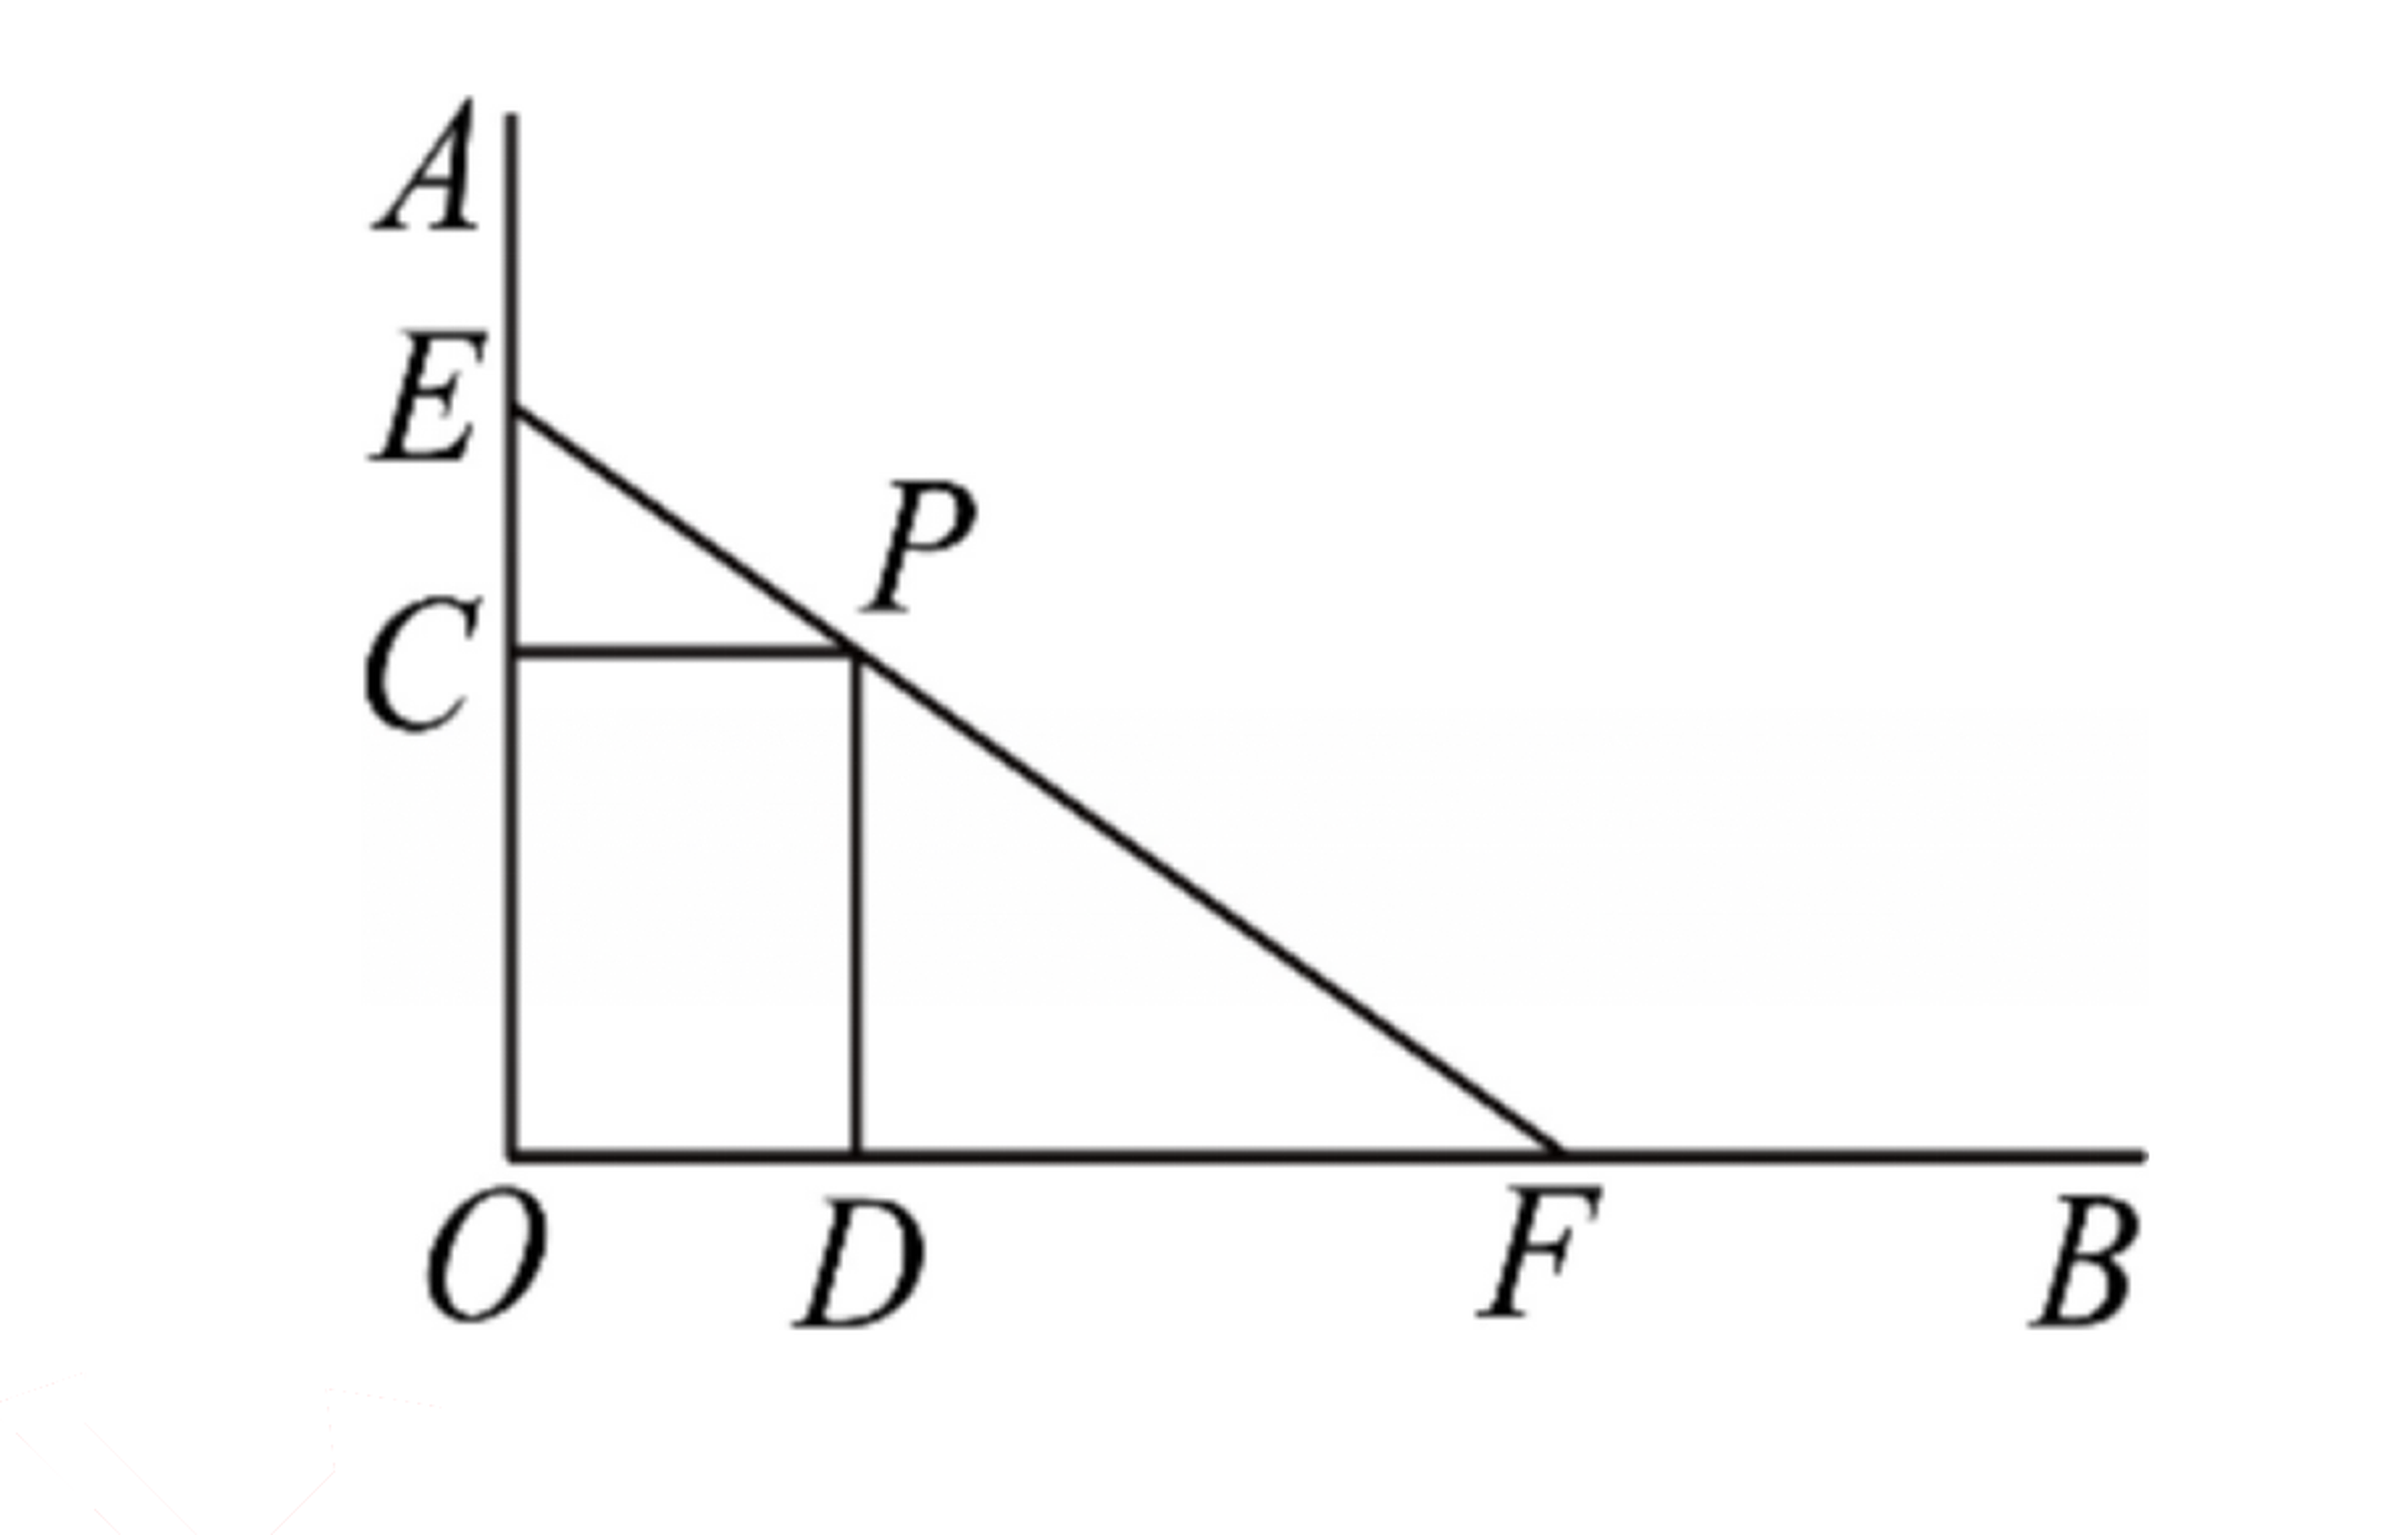
\includegraphics[width=0.32\textwidth]{figures/gao131_q19.png}
\end{center}

\ifanswer
\solbegin
\step{(1) 由题意得 $x\leq60$，}
\step{$\triangle PCE\sim\triangle FDP$，所以 $\dfrac{EC}{CP}=\dfrac{PD}{DF}$，即 $\dfrac{x}{25}=\dfrac{40}{DF}$，得 $DF=\dfrac{1000}{x}$m，}
\step{所以 $OF=OD+DF=\left(25+\dfrac{1000}{x}\right)$m，}
\step{所以 $25+\dfrac{1000}{x}\leq100$，解得 $x\geq\dfrac{40}{3}$；}
\step{综上，$\dfrac{40}{3}\leq x\leq60$；}
\step{(2) 由 $OE=OC+CE=(40+x)$m，}
\step{所以 $S=\dfrac12 OF\cdot OE=\dfrac12\left(25+\dfrac{1000}{x}\right)(40+x)$}
\step{$=\dfrac12\left(1000+25x+\dfrac{40000}{x}+1000\right)$m$^2$，}
\step{由基本不等式得 $S\geq\dfrac12\left(2000+2\sqrt{25x\cdot\dfrac{40000}{x}}\right)=2000$m$^2$，}
\step{当且仅当 $25x=\dfrac{40000}{x}$，即 $x=40$ 时取等号，}
\step{故 $EC=40$m 时，$S$ 取得最小值，为 $2000$m$^2$.}
\solend
\fi

\item 已知 $a\in\R$，函数 $y=ax^2+(3a+2)x+2a+3$.

(1) 当 $a=1$ 时，函数 $y=ax^2+(3a+2)x+2a+3$ 的图象与 $x$ 轴交于 $A(x_1,0)$，$B(x_2,0)$ 两点，求 $x_1^3+x_2^3$；

(2) 若关于 $x$ 的不等式 $ax^2+(3a+2)x+2a+3>2x$ 的解集为 $\R$，求实数 $a$ 的取值范围；

(3) 求关于 $x$ 的不等式 $y\geq1$ 的解集.

\ifanswer
\solbegin
\step{(1) 函数 $y=ax^2+(3a+2)x+2a+3$，当 $a=1$ 时，$y=x^2+5x+5$，}
\step{因为 $y=x^2+5x+5$ 的图象与 $x$ 轴交于 $A(x_1,0)$，$B(x_2,0)$ 两点，}
\step{即 $x^2+5x+5=0$ 的两个根为 $x_1$、$x_2$，}
\step{由根与系数的关系得 $x_1+x_2=-5$，$x_1x_2=5$，}
\step{所以 $x_1^2+x_2^2=(x_1+x_2)^2-2x_1x_2=25-10=15$，}
\step{所以 $x_1^3+x_2^3=(x_1+x_2)(x_1^2+x_2^2-x_1x_2)=-5\times(15-5)=-50$；}
\step{(2) 不等式 $ax^2+(3a+2)x+2a+3>2x$ 恒成立，得 $ax^2+3ax+2a+3>0$.}
\step{当 $a=0$ 时，$3>0$，恒成立，符合题意；}
\step{当 $a\neq0$ 时，若 $a<0$，二次函数 $ax^2+3ax+2a+3$ 开口向下，}
\step{一定存在小于零的部分，故不满足题意；}
\step{当 $a>0$ 时，若使 $ax^2+3ax+2a+3>0$ 恒成立，}
\step{只需 $\Delta=(3a)^2-4\times a\times(2a+3)=a^2-12a<0$，解得 $0<a<12$，}
\step{综上所述，$a$ 的取值范围为 $0\leq a<12$.}
\step{(3) 由 $y\geq1$，得 $ax^2+(3a+2)x+2a+3\geq1$，}
\step{即 $ax^2+(3a+2)x+2a+2\geq0$，即 $(ax+2a+2)(x+1)\geq0$，}
\step{当 $a=0$ 时，$2x+2\geq0$，解得 $x\geq-1$，}
\step{当 $a\neq0$ 时，}
\step{方程 $ax^2+(3a+2)x+2a+2=0$ 即为 $(x+1)(ax+2a+2)=0$，}
\step{解得 $x=-1$ 或 $x=-2-\dfrac2a$，令 $-1=-2-\dfrac2a$，即 $a=-2$，}
\step{当 $a>0$ 时，$-2-\dfrac2a<-1$，}
\step{不等式 $ax^2+(3a+2)x+2a+2\geq0$ 即为 $\left(x+\dfrac{2a+2}a\right)(x+1)\geq0$，}
\step{解得 $x\leq-2-\dfrac2a$ 或 $x\geq-1$；}
\step{当 $a<0$ 时，当 $-2-\dfrac2a<-1$，即 $a<-2$ 时，}
\step{不等式 $ax^2+(3a+2)x+2a+2\geq0$，即为 $\left(x+\dfrac{2a+2}a\right)(x+1)\leq0$，}
\step{解得 $-2-\dfrac2a\leq x\leq-1$；}
\step{当 $-2-\dfrac2a=-1$，即 $a=-2$，}
\step{不等式 $ax^2+(3a+2)x+2a+2\geq0$ 即为 $-2x^2-4x-2\geq0$，解得 $x=-1$，}
\step{当 $-2-\dfrac2a>-1$，即 $-2<a<0$ 时，}
\step{不等式 $ax^2+(3a+2)x+2a+2\geq0$ 即为 $\left(x+\dfrac{2a+2}a\right)(x+1)\leq0$，}
\step{解得 $-1\leq x\leq-2-\dfrac2a$，}
\step{综上所述，当 $a=0$ 时，解集为 $\{x\mid x\geq-1\}$；}
\step{当 $a>0$ 时，解集为 $\{x\mid x\leq-2-\dfrac2a$ 或 $x\geq-1\}$；}
\step{当 $a<-2$ 时，解集为 $\{x\mid -2-\dfrac2a\leq x\leq-1\}$；}
\step{当 $a=-2$ 时，解集为 $\{x\mid x=-1\}$；}
\step{当 $-2<a<0$ 时，解集为 $\{x\mid -1\leq x\leq-2-\dfrac2a\}$.}
\solend
\fi

\item 仔细阅读以下材料：【已知 $a$、$b\in(0,+\infty)$，$a+b=1$，求 $y=\dfrac1a+\dfrac2b$ 的最小值.

$y=\dfrac1a+\dfrac2b=\left(\dfrac1a+\dfrac2b\right)(a+b)=\dfrac ba+\dfrac{2a}b+3\geq3+2\sqrt2$，当且仅当 $\dfrac ba=\dfrac{2a}b$，即 $a=\sqrt2-1$，$b=2-\sqrt2$ 时取得等号，则 $y=\dfrac1a+\dfrac2b$ 的最小值为 $3+2\sqrt2$.

另 $y=\dfrac1a+\dfrac2b=\dfrac{a+b}a+\dfrac{2(a+b)}b=\dfrac ba+\dfrac{2a}b+3\geq3+2\sqrt2$，当且仅当 $\dfrac ba=\dfrac{2a}b$，即 $a=\sqrt2-1$，$b=2-\sqrt2$ 时取得等号，则 $y=\dfrac1a+\dfrac2b$ 的最小值为 $3+2\sqrt2$.】参考上述解法，求解下列问题.

(1) 若正实数 $x$、$y$ 满足 $x+y=1$，求 $\dfrac2x+\dfrac3y$ 的最小值；

(2) 已知 $x\in\left(0,\dfrac12\right)$，求 $t=\dfrac1x+\dfrac8{1-2x}$ 的最小值，并写出此时 $x$ 的值；

(3) 已知 $a$、$b\in(0,+\infty)$，$a+2b=1$，求 $p=\dfrac1{3a+4b}+\dfrac1{a+3b}$ 的最小值.

\ifanswer
\solbegin
\step{(1) 因为 $x>0,y>0$，且 $x+y=1$，}
\step{所以 $\dfrac2x+\dfrac3y=\left(\dfrac2x+\dfrac3y\right)(x+y)=2+\dfrac{2y}x+\dfrac{3x}y+3=5+\dfrac{2y}x+\dfrac{3x}y$，}
\step{由基本不等式得 $\dfrac{2y}x+\dfrac{3x}y\geq2\sqrt{\dfrac{2y}x\cdot\dfrac{3x}y}=2\sqrt6$，}
\step{当且仅当 $\dfrac{2y}x=\dfrac{3x}y$，即 $2y^2=3x^2$ 时，等号成立，}
\step{又因为 $x>0,y>0$ 且 $x+y=1$，此时 $x=\sqrt6-2,y=3-\sqrt6$，}
\step{所以 $\dfrac2x+\dfrac3y\geq5+2\sqrt6$，故 $\dfrac2x+\dfrac3y$ 的最小值为 $5+2\sqrt6$.}
\step{(2) 由 $0<x<\dfrac12$，则 $t=\dfrac1x+\dfrac8{1-2x}=\dfrac{2(1-2x+2x)}{2x}+\dfrac{8(1-2x+2x)}{1-2x}$}
\step{$=10+\dfrac{2\cdot(1-2x)}{2x}+\dfrac{8\cdot2x}{1-2x}\geq10+2\sqrt{\dfrac{2\cdot(1-2x)}{2x}\cdot\dfrac{8\cdot2x}{1-2x}}=18$，}
\step{当且仅当 $\dfrac{2\cdot(1-2x)}{2x}=\dfrac{8\cdot2x}{1-2x}$，即 $x=\dfrac16$ 时等号成立；}
\step{(3) 由 $a$、$b>0$，$a+2b=1$，则 $a=1-2b>0$，即 $0<b<\dfrac12$，}
\step{所以 $p=\dfrac1{3a+4b}+\dfrac1{a+3b}=\dfrac1{3a+6b-2b}+\dfrac1{a+2b+b}=\dfrac1{3-2b}+\dfrac1{1+b}$}
\step{$=\dfrac1{3-2b}+\dfrac2{2+2b}$，显然 $3-2b$、$2+2b>0$，}
\step{所以 $p=\dfrac15\cdot(3-2b+2+2b)\cdot\left(\dfrac1{3-2b}+\dfrac2{2+2b}\right)=\dfrac15\left[3+\dfrac{2+2b}{3-2b}+\dfrac{2(3-2b)}{2+2b}\right]$}
\step{$\geq\dfrac15\left[3+2\sqrt{\dfrac{2+2b}{3-2b}\cdot\dfrac{2(3-2b)}{2+2b}}\right]=\dfrac{3+2\sqrt2}5$，}
\step{当且仅当 $\dfrac{2+2b}{3-2b}=\dfrac{2(3-2b)}{2+2b}$，}
\step{即 $b=\dfrac{8-5\sqrt2}2$，$a=5\sqrt2-7$ 时等号成立.}
\solend
\fi

\end{enumerate}

\end{document}
"
%
% 原始材料：微信公众号"魔都数学加油站"文章，作者破晓，2026-11-13 18:18 发布；
% 连载"27学年高一131"，原文标题"27学年高一131——2026-2027年上海市六十中学高一上期中"；
% 原文链接：https://mp.weixin.qq.com/s/Nrbp3Uvt-sOGnOp4MEHemA。
% 正文为 11 张 PNG 页（01—05、09—11 为 2560x3620，06—08 为 4762x6735），
% 题目下印有【解析】或【答案】，为讲评版。题目、解析均据原图转录；
% 卷面粉红色水印"魔都数学加油站"及公众号页脚未录入。全卷仅第 19 题有 1 幅插图
% （矩形 OCPD 与小路 EF 的示意图），取 07.png 截图去水印。
%
% 卷首标题：原卷印作"2026-2027 年六十中学高一上期中"（公众号标题中的"上海市"
% 卷面标题行没有，本稿照卷面），年份区间按全稿惯例排 en dash；原卷未印副标题，
% 本卷为期中卷、跨集合与常用逻辑用语／不等式／函数三章，按题目内容标为
% "集合与常用逻辑用语、不等式、函数"（与 125／126／128／129 同期中卷口径相同）：
% 集合与逻辑见 Q3、Q4、Q7、Q13、Q17，不等式见 Q8、Q10、Q12、Q14、Q15、Q16、Q19、
% Q20、Q21，函数（指数／对数／幂函数、基本不等式应用）见 Q5、Q6、Q9、Q11、Q18、Q21。
%
% 题号体例：本卷共 19 题——一、填空题 3—12（10 题）、二、选择题 13—16（4 题）、
% 三、解答题 17—21（5 题）。三节分别 \setcounter{enumi}{2}／{12}／{16}。
%
% 与原卷的排版差异：
%   ① 原文从第 3 题起，本稿保留原题号（见上"题号体例"）；
%   ② 原卷每题下直接印【解析】／【答案】，本稿按全稿惯例置于答案版；第 3、4 题只印
%      【答案】，另提 \ans{}；第 13—16 题答案在解析末句"故选 …"，题干括号内留空、
%      不另提 \ans{}；其余各题印【解析】、无独立答案段；
%   ③ 原卷未印副标题，本稿按"知识模块"口径补出；
%   ④ 原卷填空横线按全稿惯例排为 \blankline[4.4em]；选择题括号排 \mbox{（\quad）}、
%      选项段前按惯例加 \keepwithprev；解答题不留作答区（原卷为讲评版，与 109—129 同）；
%   ⑤ 原卷数集排斜体 $R$／$N$，按全稿惯例改 \R／\N；绝对值排 \lvert…\rvert，
%      集合描述竖线排 \mid；不等号按全稿惯例排 \leqslant／\geqslant；
%   ⑥ 子题标号 (1)(2)(3) 原卷用半角括号，照录；圈数字 ①② 照录；
%   ⑦ 原卷第 19 题插图浮排在第 07 页题干右侧，本稿按体例就近置于题干"如图"之后
%      （居中 \includegraphics），图取原卷 07 页截图去水印；题前按惯例加
%      \needvspace{7cm} 守卫（照 高一120／127／129 成例），保证"题干 + 图"整块不被页边界切开；
%   ⑧ 原卷 Q9 题干跨 01—02 页、Q15 解析跨 03—04 页、Q16 材料跨 04—05 页、
%      Q17 题干跨 05—06 页、Q20 解析跨 08—09 页、Q21 解析跨 09—11 页，
%      本稿按题合并连续排版；末页第 11 页为 Q21 (3) 解析的续尾，按实际印刷行单列。
%   ⑨ 第 16 题材料英文括注原卷印作 (Cauchy – SchwarzInequality)（长横、Schwarz 与
%      Inequality 斜体连排无空格），本稿按全稿英文专名惯例排 \emph{(Cauchy-Schwarz Inequality)}；
%      第 15 题解析 B、D 两行原卷各印一步含 \lg m 的换底繁分数（2026-11-13 回原图核对补回，
%      本稿初转曾顺手去重跳过该步）。
%
% 判别式字形：第 20 题 (2) 解析 $\Delta=(3a)^2-4\times a\times(2a+3)=a^2-12a<0$
%   原卷排三角形（等腰、高；回 08.png 放大核对），照录 \Delta；全卷判别式仅此一处
%   （\triangle 另作第 19 题「$\triangle PCE\sim\triangle FDP$」的几何三角形记号）。
%
% 子集符号：第 17 题 (2) 解析 $P\subseteq Q$ 印带下划线，照录 \subseteq；
%   全卷未出现单线 \subset。
%
% 原卷存疑照录：
%   第 11 题解析末两式作 $\dfrac{2+m+\frac1n}{2n+2}=\dfrac{2n+mn+1}{2n+2}$，而第三式
%     分母 $\log_3 9+\log_3 2+\log_3 2=2+\frac2n$，与前一分母 $2n+2$ 不等，照录；
%   第 16 题材料 ①"对于所有实数 $x$ 和 $y$，有 $(a^2+b^2)(c^2+d^2)\geq(ac+bd)^2$"
%     句首用 $x$、$y$ 而式中用 $a$、$b$、$c$、$d$，照录；
%   第 20 题题干 (2) 作"解集为 $\R$"、解析 (2) 作"恒成立"，措辞不同，照录；
%   第 21 题材料把同一道题用两种解法连印两遍（"另 $y=\frac1a+\frac2b=\dots$"），照录；
%   第 21 题 (3) 解析末句"即 $b=\frac{8-5\sqrt2}{2}$，$a=5\sqrt2-7$ 时等号成立"
%     未另写"故最小值为 $\frac{3+2\sqrt2}{5}$"，照录；
%   第 12 题解析"所以 $e^a+e^b>e^c, a+b>c$"、第 8 题解析"$a>0$，$b>0$"、
%     第 18 题 (2)"$4x^2-4x+1<x^2+4x+4$，解得 $-\frac13<x<3$"等处数学式内
%     半角逗号，照录；
%   第 15 题解析用 $\lg$ 记常用对数（$\lg m$、$\lg 3$、$\lg 5$、$\lg 15$），照录。
%
% 行数复核：逐题数 \step 条数，合计 119 条（Q3：0；Q4：0；Q5：1；Q6：1；Q7：2；
% Q8：2；Q9：1；Q10：1；Q11：2；Q12：6；Q13：2；Q14：3；Q15：14；Q16：10；
% Q17：4；Q18：8；Q19：11；Q20：35；Q21：16），与原卷印刷行逐题相等
% （cases 块作一个印刷行计）。第 3、4 题只印【答案】，提 \ans{}，不计入 \step 账；
% 四道选择题答案均在解析末句，括号内留空、不另提 \ans{}。
%
\documentclass[a4paper,11pt]{article}
\usepackage{common}

\begin{document}

\examtitlest[3]{2026--2027 年六十中学高一上期中}{集合与常用逻辑用语、不等式、函数}

\bigsec{一、填空题}

\begin{enumerate}
\setcounter{enumi}{2}

\item 已知集合 $A=(0,4),B=[2,5]$，则 $A\cup B=$\blankline[4.4em].

\ifanswer
\ans{$(0,5]$}
\fi

\item 陈述句“$x=2$ 或 $y=3$”的否定形式为\blankline[4.4em].

\ifanswer
\ans{$x\neq2$ 且 $y\neq3$}
\fi

\item 函数 $y=a^{x-2}+15(a>0$ 且 $a\neq1)$ 的图象恒过定点的坐标为\blankline[4.4em].

\ifanswer
\solbegin
\step{函数 $y=a^{x-2}+15$ 的图象恒过定点 $A(2,16)$.}
\solend
\fi

\item 用有理数指数幂的形式来化简：$\dfrac{\sqrt{a\cdot\sqrt[3]{a^4}}}{\left(a^{\frac13}\right)^2}=$\blankline[4.4em].

\ifanswer
\solbegin
\step{原式 $=\dfrac{\sqrt{a\cdot a^{\frac43}}}{a^{\frac23}}=\dfrac{\sqrt{a^{\frac73}}}{a^{\frac23}}=\dfrac{a^{\frac76}}{a^{\frac23}}=a^{\frac76-\frac23}=a^{\frac12}(a>0)$.}
\solend
\fi

\item 已知集合 $A=\left\{x\mid \dfrac6{6-x}\in\N\text{ 且 }x\in\N\right\}$，则用列举法表示集合 $A=$\blankline[4.4em].

\ifanswer
\solbegin
\step{当 $x=0$ 时，$\dfrac6{6-0}=1\in\N$，当 $x=3$ 时，$\dfrac6{6-3}=2\in\N$，}
\step{当 $x=4$ 时，$\dfrac6{6-4}=3\in\N$，当 $x=5$ 时，$\dfrac6{6-5}=6\in\N$，故 $A=\{0,3,4,5\}$.}
\solend
\fi

\item 已知 $a>0$，$b>0$，且 $ab=\dfrac12$，则 $\dfrac1a+\dfrac8b$ 的最小值是\blankline[4.4em].

\ifanswer
\solbegin
\step{$a>0$，$b>0$，且 $ab=\dfrac12$，则 $\dfrac1a+\dfrac8b\geq2\sqrt{\dfrac8{ab}}=8$，}
\step{当且仅当 $\dfrac1a=\dfrac8b$，即 $a=\dfrac14,b=2$ 时取等号，故最小值为 $8$.}
\solend
\fi

\item 心理学家有时用函数 $L(t)=A(1-e^{-kt})$ 测定在时间 $t$（单位：$min$）内能够记忆的量 $L$，其中 $A$ 表示需要记忆的量，$k$ 表示记忆率. 假设一个学生需要记忆的量为 $200$ 个单词，此时 $L$ 表示在时间 $t$ 内该生能够记忆的单词个数. 已知该生在 $5min$ 内能够记忆 $20$ 个单词，则 $k$ 的值约为\blankline[4.4em]（结果保留四位小数）.

\ifanswer
\solbegin
\step{由题意得 $200(1-e^{-5k})=20$，所以 $e^{-5k}=0.9$，解得 $k\approx0.0211$.}
\solend
\fi

\item 设 $x\in\R$，方程 $\lvert 3x-2\rvert+\lvert 1-x\rvert=\lvert 2x-1\rvert$ 的解集是\blankline[4.4em].

\ifanswer
\solbegin
\step{由三角不等式得 $(3x-2)(1-x)\geq0$，故解集是 $\left[\dfrac23,1\right]$.}
\solend
\fi

\item 已知 $3^m=5$，$n=\log_2 3$，则 $\log_{36}90$ 可用 $m$、$n$ 表示为\blankline[4.4em].

\ifanswer
\solbegin
\step{由 $3^m=5$，又 $n=\log_2 3$，得 $m=\log_3 5$，$\log_3 2=\dfrac{\log_2 2}{\log_2 3}=\dfrac1n$，}
\step{所以 $\log_{36}90=\dfrac{\log_3 90}{\log_3 36}=\dfrac{\log_3 9+\log_3 2+\log_3 5}{\log_3 9+\log_3 2+\log_3 2}=\dfrac{2+m+\frac1n}{2n+2}=\dfrac{2n+mn+1}{2n+2}$.}
\solend
\fi

\item 若定义域为 $I=(0,m]$ 的函数 $f(x)=e^x$ 满足：对任意能构成三角形三边长的实数 $a$、$b$、$c\in I$，均有 $f(a)$、$f(b)$、$f(c)$ 也能构成三角形三边长，则 $m$ 的最大值为\blankline[4.4em].

\ifanswer
\solbegin
\step{$f(x)=e^x$ 在 $I=(0,m]$ 上严格增，所以 $f(x)\in(1,e^m]$，不妨设 $0<a\leq b\leq c$，}
\step{因为对任意能构成三角形三边长的实数 $a,b,c\in I$，均有 $f(a)$，$f(b)$，$f(c)$}
\step{也能构成三角形三边长，所以 $e^a+e^b>e^c, a+b>c$，}
\step{因为 $e^a+e^b\geq2\sqrt{e^ae^b}=2\sqrt{e^{a+b}}>e^c$，所以 $4e^{a+b}>e^{2c}$，}
\step{因为对任意 $a,b,c\in I$ 都成立，所以 $4e^c\geq e^{2c}$，所以 $e^c\leq4$，所以 $c\leq\ln4$，}
\step{所以 $m\leq\ln4$，所以 $m$ 的最大值为 $\ln4$.}
\solend
\fi

\end{enumerate}

\bigsec{二、选择题}

\begin{enumerate}
\setcounter{enumi}{12}

\item 已知 $m,n$ 是非零自然数，命题 $\alpha:mn$ 是奇数，命题 $\beta:m$ 或 $n$ 是奇数，则 $\alpha$ 是 $\beta$ 的\mbox{（\quad）}

\keepwithprev
A. 充分非必要条件\qquad\qquad B. 必要非充分条件

C. 充要条件\qquad\qquad D. 既非充分又非必要条件

\ifanswer
\solbegin
\step{$mn$ 是奇数 $\Leftrightarrow$ $m$、$n$ 都是奇数，所以 $\alpha$ 能推出 $\beta$，充分性成立，}
\step{但 $\beta$ 推不出 $\alpha$，必要性不成立，所以 $\alpha$ 是 $\beta$ 的充分非必要条件. 故选 $A$.}
\solend
\fi

\item 关于 $x$ 的不等式 $x^2-mx+n+5\leq0$ 的解集是 $[1,8]$，那么 $\log_m n=$\mbox{（\quad）}

\keepwithprev
A. $\dfrac13$\qquad\qquad B. $-3$\qquad\qquad C. $-2$\qquad\qquad D. $\dfrac12$

\ifanswer
\solbegin
\step{由题意得 $x^2-mx+n+5=0$ 的解为 $1$，$8$，}
\step{由根与系数的关系得 $\begin{cases}1+8=m\\1\times8=n+5\end{cases}$，解得 $m=9$，$n=3$，}
\step{所以 $\log_m n=\log_9 3=\dfrac12\log_3 3=\dfrac12$. 故选 $D$.}
\solend
\fi

\item 已知正实数 $x$、$y$、$z$ 满足 $3^x=5^y=15^z$，则下列说法中不正确的是\mbox{（\quad）}

\keepwithprev
A. $\dfrac1x+\dfrac1y=\dfrac1z$\qquad\qquad B. $x+y>2z$\qquad\qquad C. $3x>5y>15z$\qquad\qquad D. $x\cdot y>4z^2$

\ifanswer
\solbegin
\step{已知正实数 $x$、$y$、$z$，则设 $3^x=5^y=15^z=m>1$，}
\step{所以 $x=\log_3 m$，$y=\log_5 m$，$z=\log_{15} m$，}
\step{对于 $A$，$\dfrac1x+\dfrac1y=\dfrac1{\log_3 m}+\dfrac1{\log_5 m}=\log_m 3+\log_m 5=\log_m 15=\dfrac1z$，故 $A$ 正确；}
\step{对于 $B$，因为 $\dfrac{x+y}{z}=\dfrac{x}{z}+\dfrac{y}{z}=\dfrac{\log_3 m}{\log_{15} m}+\dfrac{\log_5 m}{\log_{15} m}=\dfrac{\dfrac{\lg m}{\lg3}}{\dfrac{\lg m}{\lg15}}+\dfrac{\dfrac{\lg m}{\lg5}}{\dfrac{\lg m}{\lg15}}=\dfrac{\lg15}{\lg3}+\dfrac{\lg15}{\lg5}$，}
\step{$=\dfrac{\lg3+\lg5}{\lg3}+\dfrac{\lg3+\lg5}{\lg5}=2+\dfrac{\lg5}{\lg3}+\dfrac{\lg3}{\lg5}=2+\log_3 5+\log_5 3$，}
\step{又 $\log_3 5>0$，$\log_5 3>0$，所以 $2+\log_3 5+\log_5 3>2$，}
\step{所以 $\dfrac{x+y}{z}>2$，即 $x+y>2z$，故 $B$ 正确；}
\step{对于 $C$，因为 $\dfrac5x=5\log_m 3=\log_m 243$，$\dfrac3y=3\log_m 5=\log_m 125$，}
\step{所以 $\dfrac5x>\dfrac3y$，即 $3x<5y$，故 $C$ 错误；}
\step{对于 $D$，$\dfrac{xy}{z^2}=\dfrac{x}{z}\cdot\dfrac{y}{z}=\dfrac{\log_3 m}{\log_{15} m}\cdot\dfrac{\log_5 m}{\log_{15} m}=\dfrac{\dfrac{\lg m}{\lg3}}{\dfrac{\lg m}{\lg15}}\cdot\dfrac{\dfrac{\lg m}{\lg5}}{\dfrac{\lg m}{\lg15}}=\dfrac{\lg15}{\lg3}\cdot\dfrac{\lg15}{\lg5}$}
\step{$=\dfrac{\lg3+\lg5}{\lg3}\cdot\dfrac{\lg3+\lg5}{\lg5}=\left(1+\dfrac{\lg5}{\lg3}\right)\left(1+\dfrac{\lg3}{\lg5}\right)=2+\dfrac{\lg5}{\lg3}+\dfrac{\lg3}{\lg5}$}
\step{$\geq2+2\sqrt{\dfrac{\lg5}{\lg3}\cdot\dfrac{\lg3}{\lg5}}=2+2=4$，又 $\lg3\neq\lg5$，故等号不成立，}
\step{所以 $\dfrac{xy}{z^2}>4$，即 $xy>4z^2$，故 $D$ 正确.}
\step{故选 $C$.}
\solend
\fi

\item 柯西不等式 \emph{(Cauchy-Schwarz Inequality)} 是一种在数学和物理学中广泛使用的不等式，它是由法国数学家奥古斯丁$\cdot$路易$\cdot$柯西提出的，柯西不等式可以用于证明其他不等式，也可以用于解决一些数学问题. 以下是柯西不等式的原始形式：

①对于所有实数 $x$ 和 $y$，有 $(a^2+b^2)(c^2+d^2)\geq(ac+bd)^2$.

②等式条件：当且仅当 $ad-bc=0$ 时，等号成立.

例：已知 $x+2y=2$，由柯西不等式 $(x^2+y^2)(1^2+2^2)\geq(x+2y)^2$，可得 $(x^2+y^2)_{min}=\dfrac45$.

现给出以下两个命题：

①若 $a^2+b^2=1$，则 $2a+3b$ 的最大值为 $\sqrt{13}$；

②若 $1<a<3$，则 $\sqrt{a-1}+\sqrt{6-2a}$ 的最大值为 $\sqrt6$；

则运用柯西不等式，判断以下正确的选项有\mbox{（\quad）}

\keepwithprev
A. ①为真命题；②为真命题\qquad\qquad B. ①为真命题；②为假命题

C. ①为假命题；②为真命题\qquad\qquad D. ①为假命题；②为假命题

\ifanswer
\solbegin
\step{由柯西不等式得 $(a^2+b^2)(2^2+3^2)\geq(2a+3b)^2$.}
\step{因为 $a^2+b^2=1$，所以 $(2^2+3^2)\geq(2a+3b)^2$，即 $13\geq(2a+3b)^2$，}
\step{所以 $-\sqrt{13}\leq2a+3b\leq\sqrt{13}$，则 $(2a+3b)_{max}=\sqrt{13}$，}
\step{当且仅当 $3a=2b$ 时取等号，故①正确.}
\step{令 $x=\sqrt{a-1}$，$y=\sqrt{3-a}$，则 $x^2+y^2=a-1+3-a=2$，}
\step{由柯西不等式得 $(\sqrt{a-1}+\sqrt{6-2a})^2=(\sqrt{a-1}+\sqrt2\cdot\sqrt{3-a})^2=(x+\sqrt2 y)^2$}
\step{$\leq[1^2+(\sqrt2)^2](x^2+y^2)$，}
\step{因为 $x^2+y^2=2$，所以 $(\sqrt{a-1}+\sqrt{6-2a})^2\leq6$，}
\step{当且仅当 $\sqrt{3-a}=\sqrt2\sqrt{a-1}$ 取等号，所以 $\sqrt{a-1}+\sqrt{6-2a}\leq\sqrt6$，故②正确.}
\step{故选 $A$.}
\solend
\fi

\end{enumerate}

\bigsec{三、解答题}

\begin{enumerate}
\setcounter{enumi}{16}

\item 已知集合 $P=\left\{x\mid \dfrac{3x-1}{x+2}<1\right\}$，集合 $Q=\{x\mid\lvert x-a\rvert\leq2\}$.

(1) 求集合 $P$；

(2) 若“$x\in P$”是“$x\in Q$”的充分非必要条件，求实数 $a$ 的取值范围.

\ifanswer
\solbegin
\step{(1) 集合 $P=\left\{x\mid \dfrac{3x-1}{x+2}<1\right\}$，得 $\dfrac{2x-3}{x+2}<0$，解得 $P=\left(-2,\dfrac32\right)$.}
\step{(2) 集合 $Q=\{x\mid\lvert x-a\rvert\leq2\}=\{x\mid a-2\leq x\leq2+a\}$，}
\step{由“$x\in P$”是“$x\in Q$”的充分非必要条件，得 $P\subseteq Q$，}
\step{得 $\begin{cases}-2\geq a-2\\\dfrac32\leq2+a\\a-2<2+a\end{cases}$，解得 $a\in\left[-\dfrac12,0\right]$.}
\solend
\fi

\item 已知幂函数 $f(x)=(m^2-4m+4)\cdot x^{2m-4}$ 在 $(-\infty,0)$ 上是严格减函数.

(1) 求函数 $y=f(x)$ 的解析式；

(2) 若 $f(1-2x)<f(x+2)$，求 $x$ 的取值范围.

\ifanswer
\solbegin
\step{(1) 由幂函数的定义得 $m^2-4m+4=1$，解得 $m=1$ 或 $3$，}
\step{当 $m=1$ 时，$f(x)=x^{-2}=\dfrac1{x^2}$，在 $(-\infty,0)$ 上严格增，不符合题意，}
\step{当 $m=3$ 时，$f(x)=x^2$，在 $(-\infty,0)$ 上严格减，符合题意，}
\step{所以 $f(x)=x^2$；}
\step{(2) 由函数 $f(x)=x^2$ 图象关于 $y$ 轴对称，且在 $[0,+\infty)$ 上严格增，}
\step{则 $f(1-2x)<f(x+2)$ 可化为 $\lvert1-2x\rvert<\lvert x+2\rvert$，}
\step{平方得 $4x^2-4x+1<x^2+4x+4$，解得 $-\dfrac13<x<3$，}
\step{所以 $x$ 的取值范围是 $\left(-\dfrac13,3\right)$.}
\solend
\fi

% 第 19 题是"题干 + 图"约 7cm 的一整块，守卫放在 \item 之前（放 \item 之后会失效）
\needvspace{7cm}
\item 如图，$OA$、$OB$ 是两条长度足够长的互相垂直的笔直小路，矩形 $OCPD$ 的顶点 $C$，$D$ 分别在 $OA$、$OB$ 上，且该矩形区域内种满了荷花. 为了让观赏者有更好的观赏体验，现计划经过点 $P$ 修一条小路 $EF$，其中点 $E$ 在小路 $OA$ 上，点 $F$ 在小路 $OB$ 上，并在 $\triangle OEF$ 区域内种满荷花. 已知 $OD=25m$，$OC=40m$，且小路 $EF$ 要完全位于一个以 $O$ 为顶点的，边长为 $100$ m 的正方形内部（包括边界）. 记 $\triangle OEF$ 的面积为 $S$m$^2$.

(1) 设 $EC=x\cdot m$，试用 $x$ 表示 $OF$，并求 $x$ 的取值范围.

(2) 当 $EC$ 的长度为多少时，$S$ 取得最小值？最小值是多少？

\begin{center}
% 图取原卷 07.png 截图去粉色水印，2.8× LANCZOS 放大
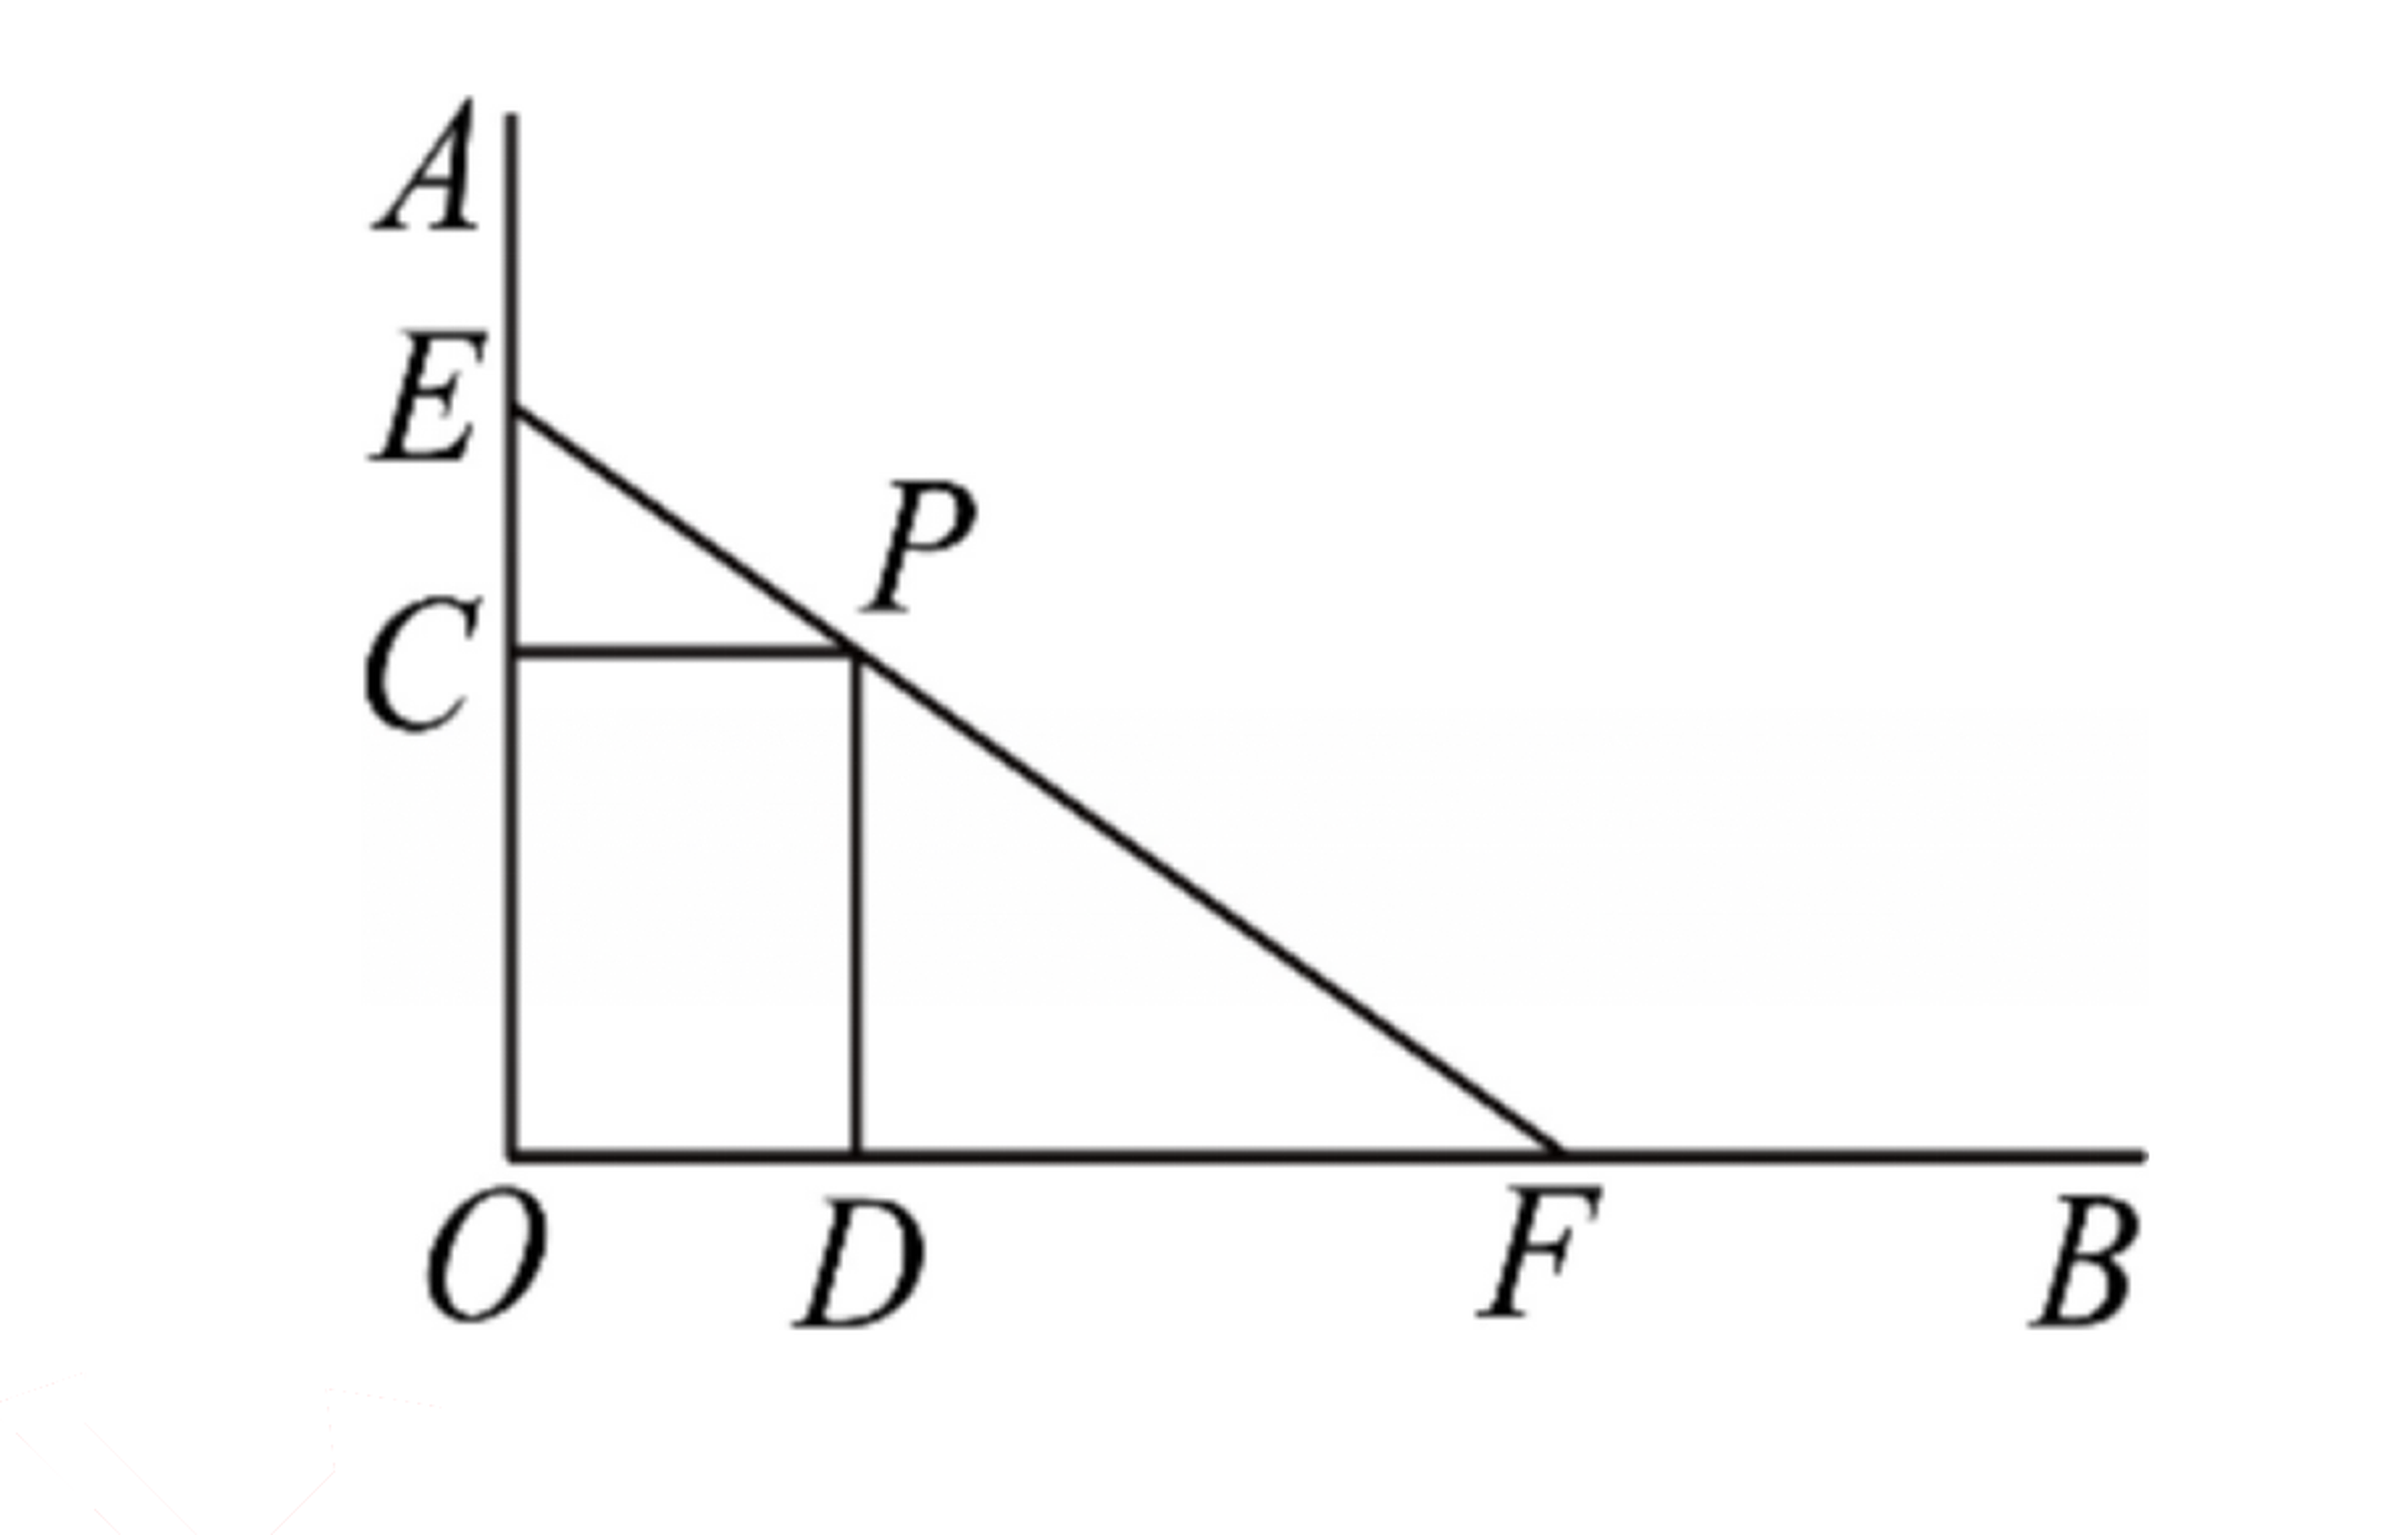
\includegraphics[width=0.32\textwidth]{figures/gao131_q19.png}
\end{center}

\ifanswer
\solbegin
\step{(1) 由题意得 $x\leq60$，}
\step{$\triangle PCE\sim\triangle FDP$，所以 $\dfrac{EC}{CP}=\dfrac{PD}{DF}$，即 $\dfrac{x}{25}=\dfrac{40}{DF}$，得 $DF=\dfrac{1000}{x}$m，}
\step{所以 $OF=OD+DF=\left(25+\dfrac{1000}{x}\right)$m，}
\step{所以 $25+\dfrac{1000}{x}\leq100$，解得 $x\geq\dfrac{40}{3}$；}
\step{综上，$\dfrac{40}{3}\leq x\leq60$；}
\step{(2) 由 $OE=OC+CE=(40+x)$m，}
\step{所以 $S=\dfrac12 OF\cdot OE=\dfrac12\left(25+\dfrac{1000}{x}\right)(40+x)$}
\step{$=\dfrac12\left(1000+25x+\dfrac{40000}{x}+1000\right)$m$^2$，}
\step{由基本不等式得 $S\geq\dfrac12\left(2000+2\sqrt{25x\cdot\dfrac{40000}{x}}\right)=2000$m$^2$，}
\step{当且仅当 $25x=\dfrac{40000}{x}$，即 $x=40$ 时取等号，}
\step{故 $EC=40$m 时，$S$ 取得最小值，为 $2000$m$^2$.}
\solend
\fi

\item 已知 $a\in\R$，函数 $y=ax^2+(3a+2)x+2a+3$.

(1) 当 $a=1$ 时，函数 $y=ax^2+(3a+2)x+2a+3$ 的图象与 $x$ 轴交于 $A(x_1,0)$，$B(x_2,0)$ 两点，求 $x_1^3+x_2^3$；

(2) 若关于 $x$ 的不等式 $ax^2+(3a+2)x+2a+3>2x$ 的解集为 $\R$，求实数 $a$ 的取值范围；

(3) 求关于 $x$ 的不等式 $y\geq1$ 的解集.

\ifanswer
\solbegin
\step{(1) 函数 $y=ax^2+(3a+2)x+2a+3$，当 $a=1$ 时，$y=x^2+5x+5$，}
\step{因为 $y=x^2+5x+5$ 的图象与 $x$ 轴交于 $A(x_1,0)$，$B(x_2,0)$ 两点，}
\step{即 $x^2+5x+5=0$ 的两个根为 $x_1$、$x_2$，}
\step{由根与系数的关系得 $x_1+x_2=-5$，$x_1x_2=5$，}
\step{所以 $x_1^2+x_2^2=(x_1+x_2)^2-2x_1x_2=25-10=15$，}
\step{所以 $x_1^3+x_2^3=(x_1+x_2)(x_1^2+x_2^2-x_1x_2)=-5\times(15-5)=-50$；}
\step{(2) 不等式 $ax^2+(3a+2)x+2a+3>2x$ 恒成立，得 $ax^2+3ax+2a+3>0$.}
\step{当 $a=0$ 时，$3>0$，恒成立，符合题意；}
\step{当 $a\neq0$ 时，若 $a<0$，二次函数 $ax^2+3ax+2a+3$ 开口向下，}
\step{一定存在小于零的部分，故不满足题意；}
\step{当 $a>0$ 时，若使 $ax^2+3ax+2a+3>0$ 恒成立，}
\step{只需 $\Delta=(3a)^2-4\times a\times(2a+3)=a^2-12a<0$，解得 $0<a<12$，}
\step{综上所述，$a$ 的取值范围为 $0\leq a<12$.}
\step{(3) 由 $y\geq1$，得 $ax^2+(3a+2)x+2a+3\geq1$，}
\step{即 $ax^2+(3a+2)x+2a+2\geq0$，即 $(ax+2a+2)(x+1)\geq0$，}
\step{当 $a=0$ 时，$2x+2\geq0$，解得 $x\geq-1$，}
\step{当 $a\neq0$ 时，}
\step{方程 $ax^2+(3a+2)x+2a+2=0$ 即为 $(x+1)(ax+2a+2)=0$，}
\step{解得 $x=-1$ 或 $x=-2-\dfrac2a$，令 $-1=-2-\dfrac2a$，即 $a=-2$，}
\step{当 $a>0$ 时，$-2-\dfrac2a<-1$，}
\step{不等式 $ax^2+(3a+2)x+2a+2\geq0$ 即为 $\left(x+\dfrac{2a+2}a\right)(x+1)\geq0$，}
\step{解得 $x\leq-2-\dfrac2a$ 或 $x\geq-1$；}
\step{当 $a<0$ 时，当 $-2-\dfrac2a<-1$，即 $a<-2$ 时，}
\step{不等式 $ax^2+(3a+2)x+2a+2\geq0$，即为 $\left(x+\dfrac{2a+2}a\right)(x+1)\leq0$，}
\step{解得 $-2-\dfrac2a\leq x\leq-1$；}
\step{当 $-2-\dfrac2a=-1$，即 $a=-2$，}
\step{不等式 $ax^2+(3a+2)x+2a+2\geq0$ 即为 $-2x^2-4x-2\geq0$，解得 $x=-1$，}
\step{当 $-2-\dfrac2a>-1$，即 $-2<a<0$ 时，}
\step{不等式 $ax^2+(3a+2)x+2a+2\geq0$ 即为 $\left(x+\dfrac{2a+2}a\right)(x+1)\leq0$，}
\step{解得 $-1\leq x\leq-2-\dfrac2a$，}
\step{综上所述，当 $a=0$ 时，解集为 $\{x\mid x\geq-1\}$；}
\step{当 $a>0$ 时，解集为 $\{x\mid x\leq-2-\dfrac2a$ 或 $x\geq-1\}$；}
\step{当 $a<-2$ 时，解集为 $\{x\mid -2-\dfrac2a\leq x\leq-1\}$；}
\step{当 $a=-2$ 时，解集为 $\{x\mid x=-1\}$；}
\step{当 $-2<a<0$ 时，解集为 $\{x\mid -1\leq x\leq-2-\dfrac2a\}$.}
\solend
\fi

\item 仔细阅读以下材料：【已知 $a$、$b\in(0,+\infty)$，$a+b=1$，求 $y=\dfrac1a+\dfrac2b$ 的最小值.

$y=\dfrac1a+\dfrac2b=\left(\dfrac1a+\dfrac2b\right)(a+b)=\dfrac ba+\dfrac{2a}b+3\geq3+2\sqrt2$，当且仅当 $\dfrac ba=\dfrac{2a}b$，即 $a=\sqrt2-1$，$b=2-\sqrt2$ 时取得等号，则 $y=\dfrac1a+\dfrac2b$ 的最小值为 $3+2\sqrt2$.

另 $y=\dfrac1a+\dfrac2b=\dfrac{a+b}a+\dfrac{2(a+b)}b=\dfrac ba+\dfrac{2a}b+3\geq3+2\sqrt2$，当且仅当 $\dfrac ba=\dfrac{2a}b$，即 $a=\sqrt2-1$，$b=2-\sqrt2$ 时取得等号，则 $y=\dfrac1a+\dfrac2b$ 的最小值为 $3+2\sqrt2$.】参考上述解法，求解下列问题.

(1) 若正实数 $x$、$y$ 满足 $x+y=1$，求 $\dfrac2x+\dfrac3y$ 的最小值；

(2) 已知 $x\in\left(0,\dfrac12\right)$，求 $t=\dfrac1x+\dfrac8{1-2x}$ 的最小值，并写出此时 $x$ 的值；

(3) 已知 $a$、$b\in(0,+\infty)$，$a+2b=1$，求 $p=\dfrac1{3a+4b}+\dfrac1{a+3b}$ 的最小值.

\ifanswer
\solbegin
\step{(1) 因为 $x>0,y>0$，且 $x+y=1$，}
\step{所以 $\dfrac2x+\dfrac3y=\left(\dfrac2x+\dfrac3y\right)(x+y)=2+\dfrac{2y}x+\dfrac{3x}y+3=5+\dfrac{2y}x+\dfrac{3x}y$，}
\step{由基本不等式得 $\dfrac{2y}x+\dfrac{3x}y\geq2\sqrt{\dfrac{2y}x\cdot\dfrac{3x}y}=2\sqrt6$，}
\step{当且仅当 $\dfrac{2y}x=\dfrac{3x}y$，即 $2y^2=3x^2$ 时，等号成立，}
\step{又因为 $x>0,y>0$ 且 $x+y=1$，此时 $x=\sqrt6-2,y=3-\sqrt6$，}
\step{所以 $\dfrac2x+\dfrac3y\geq5+2\sqrt6$，故 $\dfrac2x+\dfrac3y$ 的最小值为 $5+2\sqrt6$.}
\step{(2) 由 $0<x<\dfrac12$，则 $t=\dfrac1x+\dfrac8{1-2x}=\dfrac{2(1-2x+2x)}{2x}+\dfrac{8(1-2x+2x)}{1-2x}$}
\step{$=10+\dfrac{2\cdot(1-2x)}{2x}+\dfrac{8\cdot2x}{1-2x}\geq10+2\sqrt{\dfrac{2\cdot(1-2x)}{2x}\cdot\dfrac{8\cdot2x}{1-2x}}=18$，}
\step{当且仅当 $\dfrac{2\cdot(1-2x)}{2x}=\dfrac{8\cdot2x}{1-2x}$，即 $x=\dfrac16$ 时等号成立；}
\step{(3) 由 $a$、$b>0$，$a+2b=1$，则 $a=1-2b>0$，即 $0<b<\dfrac12$，}
\step{所以 $p=\dfrac1{3a+4b}+\dfrac1{a+3b}=\dfrac1{3a+6b-2b}+\dfrac1{a+2b+b}=\dfrac1{3-2b}+\dfrac1{1+b}$}
\step{$=\dfrac1{3-2b}+\dfrac2{2+2b}$，显然 $3-2b$、$2+2b>0$，}
\step{所以 $p=\dfrac15\cdot(3-2b+2+2b)\cdot\left(\dfrac1{3-2b}+\dfrac2{2+2b}\right)=\dfrac15\left[3+\dfrac{2+2b}{3-2b}+\dfrac{2(3-2b)}{2+2b}\right]$}
\step{$\geq\dfrac15\left[3+2\sqrt{\dfrac{2+2b}{3-2b}\cdot\dfrac{2(3-2b)}{2+2b}}\right]=\dfrac{3+2\sqrt2}5$，}
\step{当且仅当 $\dfrac{2+2b}{3-2b}=\dfrac{2(3-2b)}{2+2b}$，}
\step{即 $b=\dfrac{8-5\sqrt2}2$，$a=5\sqrt2-7$ 时等号成立.}
\solend
\fi

\end{enumerate}

\end{document}
"
%
% 原始材料：微信公众号"魔都数学加油站"文章，作者破晓，2026-11-13 18:18 发布；
% 连载"27学年高一131"，原文标题"27学年高一131——2026-2027年上海市六十中学高一上期中"；
% 原文链接：https://mp.weixin.qq.com/s/Nrbp3Uvt-sOGnOp4MEHemA。
% 正文为 11 张 PNG 页（01—05、09—11 为 2560x3620，06—08 为 4762x6735），
% 题目下印有【解析】或【答案】，为讲评版。题目、解析均据原图转录；
% 卷面粉红色水印"魔都数学加油站"及公众号页脚未录入。全卷仅第 19 题有 1 幅插图
% （矩形 OCPD 与小路 EF 的示意图），取 07.png 截图去水印。
%
% 卷首标题：原卷印作"2026-2027 年六十中学高一上期中"（公众号标题中的"上海市"
% 卷面标题行没有，本稿照卷面），年份区间按全稿惯例排 en dash；原卷未印副标题，
% 本卷为期中卷、跨集合与常用逻辑用语／不等式／函数三章，按题目内容标为
% "集合与常用逻辑用语、不等式、函数"（与 125／126／128／129 同期中卷口径相同）：
% 集合与逻辑见 Q3、Q4、Q7、Q13、Q17，不等式见 Q8、Q10、Q12、Q14、Q15、Q16、Q19、
% Q20、Q21，函数（指数／对数／幂函数、基本不等式应用）见 Q5、Q6、Q9、Q11、Q18、Q21。
%
% 题号体例：本卷共 19 题——一、填空题 3—12（10 题）、二、选择题 13—16（4 题）、
% 三、解答题 17—21（5 题）。三节分别 \setcounter{enumi}{2}／{12}／{16}。
%
% 与原卷的排版差异：
%   ① 原文从第 3 题起，本稿保留原题号（见上"题号体例"）；
%   ② 原卷每题下直接印【解析】／【答案】，本稿按全稿惯例置于答案版；第 3、4 题只印
%      【答案】，另提 \ans{}；第 13—16 题答案在解析末句"故选 …"，题干括号内留空、
%      不另提 \ans{}；其余各题印【解析】、无独立答案段；
%   ③ 原卷未印副标题，本稿按"知识模块"口径补出；
%   ④ 原卷填空横线按全稿惯例排为 \blankline[4.4em]；选择题括号排 \mbox{（\quad）}、
%      选项段前按惯例加 \keepwithprev；解答题不留作答区（原卷为讲评版，与 109—129 同）；
%   ⑤ 原卷数集排斜体 $R$／$N$，按全稿惯例改 \R／\N；绝对值排 \lvert…\rvert，
%      集合描述竖线排 \mid；不等号按全稿惯例排 \leqslant／\geqslant；
%   ⑥ 子题标号 (1)(2)(3) 原卷用半角括号，照录；圈数字 ①② 照录；
%   ⑦ 原卷第 19 题插图浮排在第 07 页题干右侧，本稿按体例就近置于题干"如图"之后
%      （居中 \includegraphics），图取原卷 07 页截图去水印；题前按惯例加
%      \needvspace{7cm} 守卫（照 高一120／127／129 成例），保证"题干 + 图"整块不被页边界切开；
%   ⑧ 原卷 Q9 题干跨 01—02 页、Q15 解析跨 03—04 页、Q16 材料跨 04—05 页、
%      Q17 题干跨 05—06 页、Q20 解析跨 08—09 页、Q21 解析跨 09—11 页，
%      本稿按题合并连续排版；末页第 11 页为 Q21 (3) 解析的续尾，按实际印刷行单列。
%   ⑨ 第 16 题材料英文括注原卷印作 (Cauchy – SchwarzInequality)（长横、Schwarz 与
%      Inequality 斜体连排无空格），本稿按全稿英文专名惯例排 \emph{(Cauchy-Schwarz Inequality)}；
%      第 15 题解析 B、D 两行原卷各印一步含 \lg m 的换底繁分数（2026-11-13 回原图核对补回，
%      本稿初转曾顺手去重跳过该步）。
%
% 判别式字形：第 20 题 (2) 解析 $\Delta=(3a)^2-4\times a\times(2a+3)=a^2-12a<0$
%   原卷排三角形（等腰、高；回 08.png 放大核对），照录 \Delta；全卷判别式仅此一处
%   （\triangle 另作第 19 题「$\triangle PCE\sim\triangle FDP$」的几何三角形记号）。
%
% 子集符号：第 17 题 (2) 解析 $P\subseteq Q$ 印带下划线，照录 \subseteq；
%   全卷未出现单线 \subset。
%
% 原卷存疑照录：
%   第 11 题解析末两式作 $\dfrac{2+m+\frac1n}{2n+2}=\dfrac{2n+mn+1}{2n+2}$，而第三式
%     分母 $\log_3 9+\log_3 2+\log_3 2=2+\frac2n$，与前一分母 $2n+2$ 不等，照录；
%   第 16 题材料 ①"对于所有实数 $x$ 和 $y$，有 $(a^2+b^2)(c^2+d^2)\geq(ac+bd)^2$"
%     句首用 $x$、$y$ 而式中用 $a$、$b$、$c$、$d$，照录；
%   第 20 题题干 (2) 作"解集为 $\R$"、解析 (2) 作"恒成立"，措辞不同，照录；
%   第 21 题材料把同一道题用两种解法连印两遍（"另 $y=\frac1a+\frac2b=\dots$"），照录；
%   第 21 题 (3) 解析末句"即 $b=\frac{8-5\sqrt2}{2}$，$a=5\sqrt2-7$ 时等号成立"
%     未另写"故最小值为 $\frac{3+2\sqrt2}{5}$"，照录；
%   第 12 题解析"所以 $e^a+e^b>e^c, a+b>c$"、第 8 题解析"$a>0$，$b>0$"、
%     第 18 题 (2)"$4x^2-4x+1<x^2+4x+4$，解得 $-\frac13<x<3$"等处数学式内
%     半角逗号，照录；
%   第 15 题解析用 $\lg$ 记常用对数（$\lg m$、$\lg 3$、$\lg 5$、$\lg 15$），照录。
%
% 行数复核：逐题数 \step 条数，合计 119 条（Q3：0；Q4：0；Q5：1；Q6：1；Q7：2；
% Q8：2；Q9：1；Q10：1；Q11：2；Q12：6；Q13：2；Q14：3；Q15：14；Q16：10；
% Q17：4；Q18：8；Q19：11；Q20：35；Q21：16），与原卷印刷行逐题相等
% （cases 块作一个印刷行计）。第 3、4 题只印【答案】，提 \ans{}，不计入 \step 账；
% 四道选择题答案均在解析末句，括号内留空、不另提 \ans{}。
%
\documentclass[a4paper,11pt]{article}
\usepackage{common}

\begin{document}

\examtitlest[3]{2026--2027 年六十中学高一上期中}{集合与常用逻辑用语、不等式、函数}

\bigsec{一、填空题}

\begin{enumerate}
\setcounter{enumi}{2}

\item 已知集合 $A=(0,4),B=[2,5]$，则 $A\cup B=$\blankline[4.4em].

\ifanswer
\ans{$(0,5]$}
\fi

\item 陈述句“$x=2$ 或 $y=3$”的否定形式为\blankline[4.4em].

\ifanswer
\ans{$x\neq2$ 且 $y\neq3$}
\fi

\item 函数 $y=a^{x-2}+15(a>0$ 且 $a\neq1)$ 的图象恒过定点的坐标为\blankline[4.4em].

\ifanswer
\solbegin
\step{函数 $y=a^{x-2}+15$ 的图象恒过定点 $A(2,16)$.}
\solend
\fi

\item 用有理数指数幂的形式来化简：$\dfrac{\sqrt{a\cdot\sqrt[3]{a^4}}}{\left(a^{\frac13}\right)^2}=$\blankline[4.4em].

\ifanswer
\solbegin
\step{原式 $=\dfrac{\sqrt{a\cdot a^{\frac43}}}{a^{\frac23}}=\dfrac{\sqrt{a^{\frac73}}}{a^{\frac23}}=\dfrac{a^{\frac76}}{a^{\frac23}}=a^{\frac76-\frac23}=a^{\frac12}(a>0)$.}
\solend
\fi

\item 已知集合 $A=\left\{x\mid \dfrac6{6-x}\in\N\text{ 且 }x\in\N\right\}$，则用列举法表示集合 $A=$\blankline[4.4em].

\ifanswer
\solbegin
\step{当 $x=0$ 时，$\dfrac6{6-0}=1\in\N$，当 $x=3$ 时，$\dfrac6{6-3}=2\in\N$，}
\step{当 $x=4$ 时，$\dfrac6{6-4}=3\in\N$，当 $x=5$ 时，$\dfrac6{6-5}=6\in\N$，故 $A=\{0,3,4,5\}$.}
\solend
\fi

\item 已知 $a>0$，$b>0$，且 $ab=\dfrac12$，则 $\dfrac1a+\dfrac8b$ 的最小值是\blankline[4.4em].

\ifanswer
\solbegin
\step{$a>0$，$b>0$，且 $ab=\dfrac12$，则 $\dfrac1a+\dfrac8b\geq2\sqrt{\dfrac8{ab}}=8$，}
\step{当且仅当 $\dfrac1a=\dfrac8b$，即 $a=\dfrac14,b=2$ 时取等号，故最小值为 $8$.}
\solend
\fi

\item 心理学家有时用函数 $L(t)=A(1-e^{-kt})$ 测定在时间 $t$（单位：$min$）内能够记忆的量 $L$，其中 $A$ 表示需要记忆的量，$k$ 表示记忆率. 假设一个学生需要记忆的量为 $200$ 个单词，此时 $L$ 表示在时间 $t$ 内该生能够记忆的单词个数. 已知该生在 $5min$ 内能够记忆 $20$ 个单词，则 $k$ 的值约为\blankline[4.4em]（结果保留四位小数）.

\ifanswer
\solbegin
\step{由题意得 $200(1-e^{-5k})=20$，所以 $e^{-5k}=0.9$，解得 $k\approx0.0211$.}
\solend
\fi

\item 设 $x\in\R$，方程 $\lvert 3x-2\rvert+\lvert 1-x\rvert=\lvert 2x-1\rvert$ 的解集是\blankline[4.4em].

\ifanswer
\solbegin
\step{由三角不等式得 $(3x-2)(1-x)\geq0$，故解集是 $\left[\dfrac23,1\right]$.}
\solend
\fi

\item 已知 $3^m=5$，$n=\log_2 3$，则 $\log_{36}90$ 可用 $m$、$n$ 表示为\blankline[4.4em].

\ifanswer
\solbegin
\step{由 $3^m=5$，又 $n=\log_2 3$，得 $m=\log_3 5$，$\log_3 2=\dfrac{\log_2 2}{\log_2 3}=\dfrac1n$，}
\step{所以 $\log_{36}90=\dfrac{\log_3 90}{\log_3 36}=\dfrac{\log_3 9+\log_3 2+\log_3 5}{\log_3 9+\log_3 2+\log_3 2}=\dfrac{2+m+\frac1n}{2n+2}=\dfrac{2n+mn+1}{2n+2}$.}
\solend
\fi

\item 若定义域为 $I=(0,m]$ 的函数 $f(x)=e^x$ 满足：对任意能构成三角形三边长的实数 $a$、$b$、$c\in I$，均有 $f(a)$、$f(b)$、$f(c)$ 也能构成三角形三边长，则 $m$ 的最大值为\blankline[4.4em].

\ifanswer
\solbegin
\step{$f(x)=e^x$ 在 $I=(0,m]$ 上严格增，所以 $f(x)\in(1,e^m]$，不妨设 $0<a\leq b\leq c$，}
\step{因为对任意能构成三角形三边长的实数 $a,b,c\in I$，均有 $f(a)$，$f(b)$，$f(c)$}
\step{也能构成三角形三边长，所以 $e^a+e^b>e^c, a+b>c$，}
\step{因为 $e^a+e^b\geq2\sqrt{e^ae^b}=2\sqrt{e^{a+b}}>e^c$，所以 $4e^{a+b}>e^{2c}$，}
\step{因为对任意 $a,b,c\in I$ 都成立，所以 $4e^c\geq e^{2c}$，所以 $e^c\leq4$，所以 $c\leq\ln4$，}
\step{所以 $m\leq\ln4$，所以 $m$ 的最大值为 $\ln4$.}
\solend
\fi

\end{enumerate}

\bigsec{二、选择题}

\begin{enumerate}
\setcounter{enumi}{12}

\item 已知 $m,n$ 是非零自然数，命题 $\alpha:mn$ 是奇数，命题 $\beta:m$ 或 $n$ 是奇数，则 $\alpha$ 是 $\beta$ 的\mbox{（\quad）}

\keepwithprev
A. 充分非必要条件\qquad\qquad B. 必要非充分条件

C. 充要条件\qquad\qquad D. 既非充分又非必要条件

\ifanswer
\solbegin
\step{$mn$ 是奇数 $\Leftrightarrow$ $m$、$n$ 都是奇数，所以 $\alpha$ 能推出 $\beta$，充分性成立，}
\step{但 $\beta$ 推不出 $\alpha$，必要性不成立，所以 $\alpha$ 是 $\beta$ 的充分非必要条件. 故选 $A$.}
\solend
\fi

\item 关于 $x$ 的不等式 $x^2-mx+n+5\leq0$ 的解集是 $[1,8]$，那么 $\log_m n=$\mbox{（\quad）}

\keepwithprev
A. $\dfrac13$\qquad\qquad B. $-3$\qquad\qquad C. $-2$\qquad\qquad D. $\dfrac12$

\ifanswer
\solbegin
\step{由题意得 $x^2-mx+n+5=0$ 的解为 $1$，$8$，}
\step{由根与系数的关系得 $\begin{cases}1+8=m\\1\times8=n+5\end{cases}$，解得 $m=9$，$n=3$，}
\step{所以 $\log_m n=\log_9 3=\dfrac12\log_3 3=\dfrac12$. 故选 $D$.}
\solend
\fi

\item 已知正实数 $x$、$y$、$z$ 满足 $3^x=5^y=15^z$，则下列说法中不正确的是\mbox{（\quad）}

\keepwithprev
A. $\dfrac1x+\dfrac1y=\dfrac1z$\qquad\qquad B. $x+y>2z$\qquad\qquad C. $3x>5y>15z$\qquad\qquad D. $x\cdot y>4z^2$

\ifanswer
\solbegin
\step{已知正实数 $x$、$y$、$z$，则设 $3^x=5^y=15^z=m>1$，}
\step{所以 $x=\log_3 m$，$y=\log_5 m$，$z=\log_{15} m$，}
\step{对于 $A$，$\dfrac1x+\dfrac1y=\dfrac1{\log_3 m}+\dfrac1{\log_5 m}=\log_m 3+\log_m 5=\log_m 15=\dfrac1z$，故 $A$ 正确；}
\step{对于 $B$，因为 $\dfrac{x+y}{z}=\dfrac{x}{z}+\dfrac{y}{z}=\dfrac{\log_3 m}{\log_{15} m}+\dfrac{\log_5 m}{\log_{15} m}=\dfrac{\dfrac{\lg m}{\lg3}}{\dfrac{\lg m}{\lg15}}+\dfrac{\dfrac{\lg m}{\lg5}}{\dfrac{\lg m}{\lg15}}=\dfrac{\lg15}{\lg3}+\dfrac{\lg15}{\lg5}$，}
\step{$=\dfrac{\lg3+\lg5}{\lg3}+\dfrac{\lg3+\lg5}{\lg5}=2+\dfrac{\lg5}{\lg3}+\dfrac{\lg3}{\lg5}=2+\log_3 5+\log_5 3$，}
\step{又 $\log_3 5>0$，$\log_5 3>0$，所以 $2+\log_3 5+\log_5 3>2$，}
\step{所以 $\dfrac{x+y}{z}>2$，即 $x+y>2z$，故 $B$ 正确；}
\step{对于 $C$，因为 $\dfrac5x=5\log_m 3=\log_m 243$，$\dfrac3y=3\log_m 5=\log_m 125$，}
\step{所以 $\dfrac5x>\dfrac3y$，即 $3x<5y$，故 $C$ 错误；}
\step{对于 $D$，$\dfrac{xy}{z^2}=\dfrac{x}{z}\cdot\dfrac{y}{z}=\dfrac{\log_3 m}{\log_{15} m}\cdot\dfrac{\log_5 m}{\log_{15} m}=\dfrac{\dfrac{\lg m}{\lg3}}{\dfrac{\lg m}{\lg15}}\cdot\dfrac{\dfrac{\lg m}{\lg5}}{\dfrac{\lg m}{\lg15}}=\dfrac{\lg15}{\lg3}\cdot\dfrac{\lg15}{\lg5}$}
\step{$=\dfrac{\lg3+\lg5}{\lg3}\cdot\dfrac{\lg3+\lg5}{\lg5}=\left(1+\dfrac{\lg5}{\lg3}\right)\left(1+\dfrac{\lg3}{\lg5}\right)=2+\dfrac{\lg5}{\lg3}+\dfrac{\lg3}{\lg5}$}
\step{$\geq2+2\sqrt{\dfrac{\lg5}{\lg3}\cdot\dfrac{\lg3}{\lg5}}=2+2=4$，又 $\lg3\neq\lg5$，故等号不成立，}
\step{所以 $\dfrac{xy}{z^2}>4$，即 $xy>4z^2$，故 $D$ 正确.}
\step{故选 $C$.}
\solend
\fi

\item 柯西不等式 \emph{(Cauchy-Schwarz Inequality)} 是一种在数学和物理学中广泛使用的不等式，它是由法国数学家奥古斯丁$\cdot$路易$\cdot$柯西提出的，柯西不等式可以用于证明其他不等式，也可以用于解决一些数学问题. 以下是柯西不等式的原始形式：

①对于所有实数 $x$ 和 $y$，有 $(a^2+b^2)(c^2+d^2)\geq(ac+bd)^2$.

②等式条件：当且仅当 $ad-bc=0$ 时，等号成立.

例：已知 $x+2y=2$，由柯西不等式 $(x^2+y^2)(1^2+2^2)\geq(x+2y)^2$，可得 $(x^2+y^2)_{min}=\dfrac45$.

现给出以下两个命题：

①若 $a^2+b^2=1$，则 $2a+3b$ 的最大值为 $\sqrt{13}$；

②若 $1<a<3$，则 $\sqrt{a-1}+\sqrt{6-2a}$ 的最大值为 $\sqrt6$；

则运用柯西不等式，判断以下正确的选项有\mbox{（\quad）}

\keepwithprev
A. ①为真命题；②为真命题\qquad\qquad B. ①为真命题；②为假命题

C. ①为假命题；②为真命题\qquad\qquad D. ①为假命题；②为假命题

\ifanswer
\solbegin
\step{由柯西不等式得 $(a^2+b^2)(2^2+3^2)\geq(2a+3b)^2$.}
\step{因为 $a^2+b^2=1$，所以 $(2^2+3^2)\geq(2a+3b)^2$，即 $13\geq(2a+3b)^2$，}
\step{所以 $-\sqrt{13}\leq2a+3b\leq\sqrt{13}$，则 $(2a+3b)_{max}=\sqrt{13}$，}
\step{当且仅当 $3a=2b$ 时取等号，故①正确.}
\step{令 $x=\sqrt{a-1}$，$y=\sqrt{3-a}$，则 $x^2+y^2=a-1+3-a=2$，}
\step{由柯西不等式得 $(\sqrt{a-1}+\sqrt{6-2a})^2=(\sqrt{a-1}+\sqrt2\cdot\sqrt{3-a})^2=(x+\sqrt2 y)^2$}
\step{$\leq[1^2+(\sqrt2)^2](x^2+y^2)$，}
\step{因为 $x^2+y^2=2$，所以 $(\sqrt{a-1}+\sqrt{6-2a})^2\leq6$，}
\step{当且仅当 $\sqrt{3-a}=\sqrt2\sqrt{a-1}$ 取等号，所以 $\sqrt{a-1}+\sqrt{6-2a}\leq\sqrt6$，故②正确.}
\step{故选 $A$.}
\solend
\fi

\end{enumerate}

\bigsec{三、解答题}

\begin{enumerate}
\setcounter{enumi}{16}

\item 已知集合 $P=\left\{x\mid \dfrac{3x-1}{x+2}<1\right\}$，集合 $Q=\{x\mid\lvert x-a\rvert\leq2\}$.

(1) 求集合 $P$；

(2) 若“$x\in P$”是“$x\in Q$”的充分非必要条件，求实数 $a$ 的取值范围.

\ifanswer
\solbegin
\step{(1) 集合 $P=\left\{x\mid \dfrac{3x-1}{x+2}<1\right\}$，得 $\dfrac{2x-3}{x+2}<0$，解得 $P=\left(-2,\dfrac32\right)$.}
\step{(2) 集合 $Q=\{x\mid\lvert x-a\rvert\leq2\}=\{x\mid a-2\leq x\leq2+a\}$，}
\step{由“$x\in P$”是“$x\in Q$”的充分非必要条件，得 $P\subseteq Q$，}
\step{得 $\begin{cases}-2\geq a-2\\\dfrac32\leq2+a\\a-2<2+a\end{cases}$，解得 $a\in\left[-\dfrac12,0\right]$.}
\solend
\fi

\item 已知幂函数 $f(x)=(m^2-4m+4)\cdot x^{2m-4}$ 在 $(-\infty,0)$ 上是严格减函数.

(1) 求函数 $y=f(x)$ 的解析式；

(2) 若 $f(1-2x)<f(x+2)$，求 $x$ 的取值范围.

\ifanswer
\solbegin
\step{(1) 由幂函数的定义得 $m^2-4m+4=1$，解得 $m=1$ 或 $3$，}
\step{当 $m=1$ 时，$f(x)=x^{-2}=\dfrac1{x^2}$，在 $(-\infty,0)$ 上严格增，不符合题意，}
\step{当 $m=3$ 时，$f(x)=x^2$，在 $(-\infty,0)$ 上严格减，符合题意，}
\step{所以 $f(x)=x^2$；}
\step{(2) 由函数 $f(x)=x^2$ 图象关于 $y$ 轴对称，且在 $[0,+\infty)$ 上严格增，}
\step{则 $f(1-2x)<f(x+2)$ 可化为 $\lvert1-2x\rvert<\lvert x+2\rvert$，}
\step{平方得 $4x^2-4x+1<x^2+4x+4$，解得 $-\dfrac13<x<3$，}
\step{所以 $x$ 的取值范围是 $\left(-\dfrac13,3\right)$.}
\solend
\fi

% 第 19 题是"题干 + 图"约 7cm 的一整块，守卫放在 \item 之前（放 \item 之后会失效）
\needvspace{7cm}
\item 如图，$OA$、$OB$ 是两条长度足够长的互相垂直的笔直小路，矩形 $OCPD$ 的顶点 $C$，$D$ 分别在 $OA$、$OB$ 上，且该矩形区域内种满了荷花. 为了让观赏者有更好的观赏体验，现计划经过点 $P$ 修一条小路 $EF$，其中点 $E$ 在小路 $OA$ 上，点 $F$ 在小路 $OB$ 上，并在 $\triangle OEF$ 区域内种满荷花. 已知 $OD=25m$，$OC=40m$，且小路 $EF$ 要完全位于一个以 $O$ 为顶点的，边长为 $100$ m 的正方形内部（包括边界）. 记 $\triangle OEF$ 的面积为 $S$m$^2$.

(1) 设 $EC=x\cdot m$，试用 $x$ 表示 $OF$，并求 $x$ 的取值范围.

(2) 当 $EC$ 的长度为多少时，$S$ 取得最小值？最小值是多少？

\begin{center}
% 图取原卷 07.png 截图去粉色水印，2.8× LANCZOS 放大
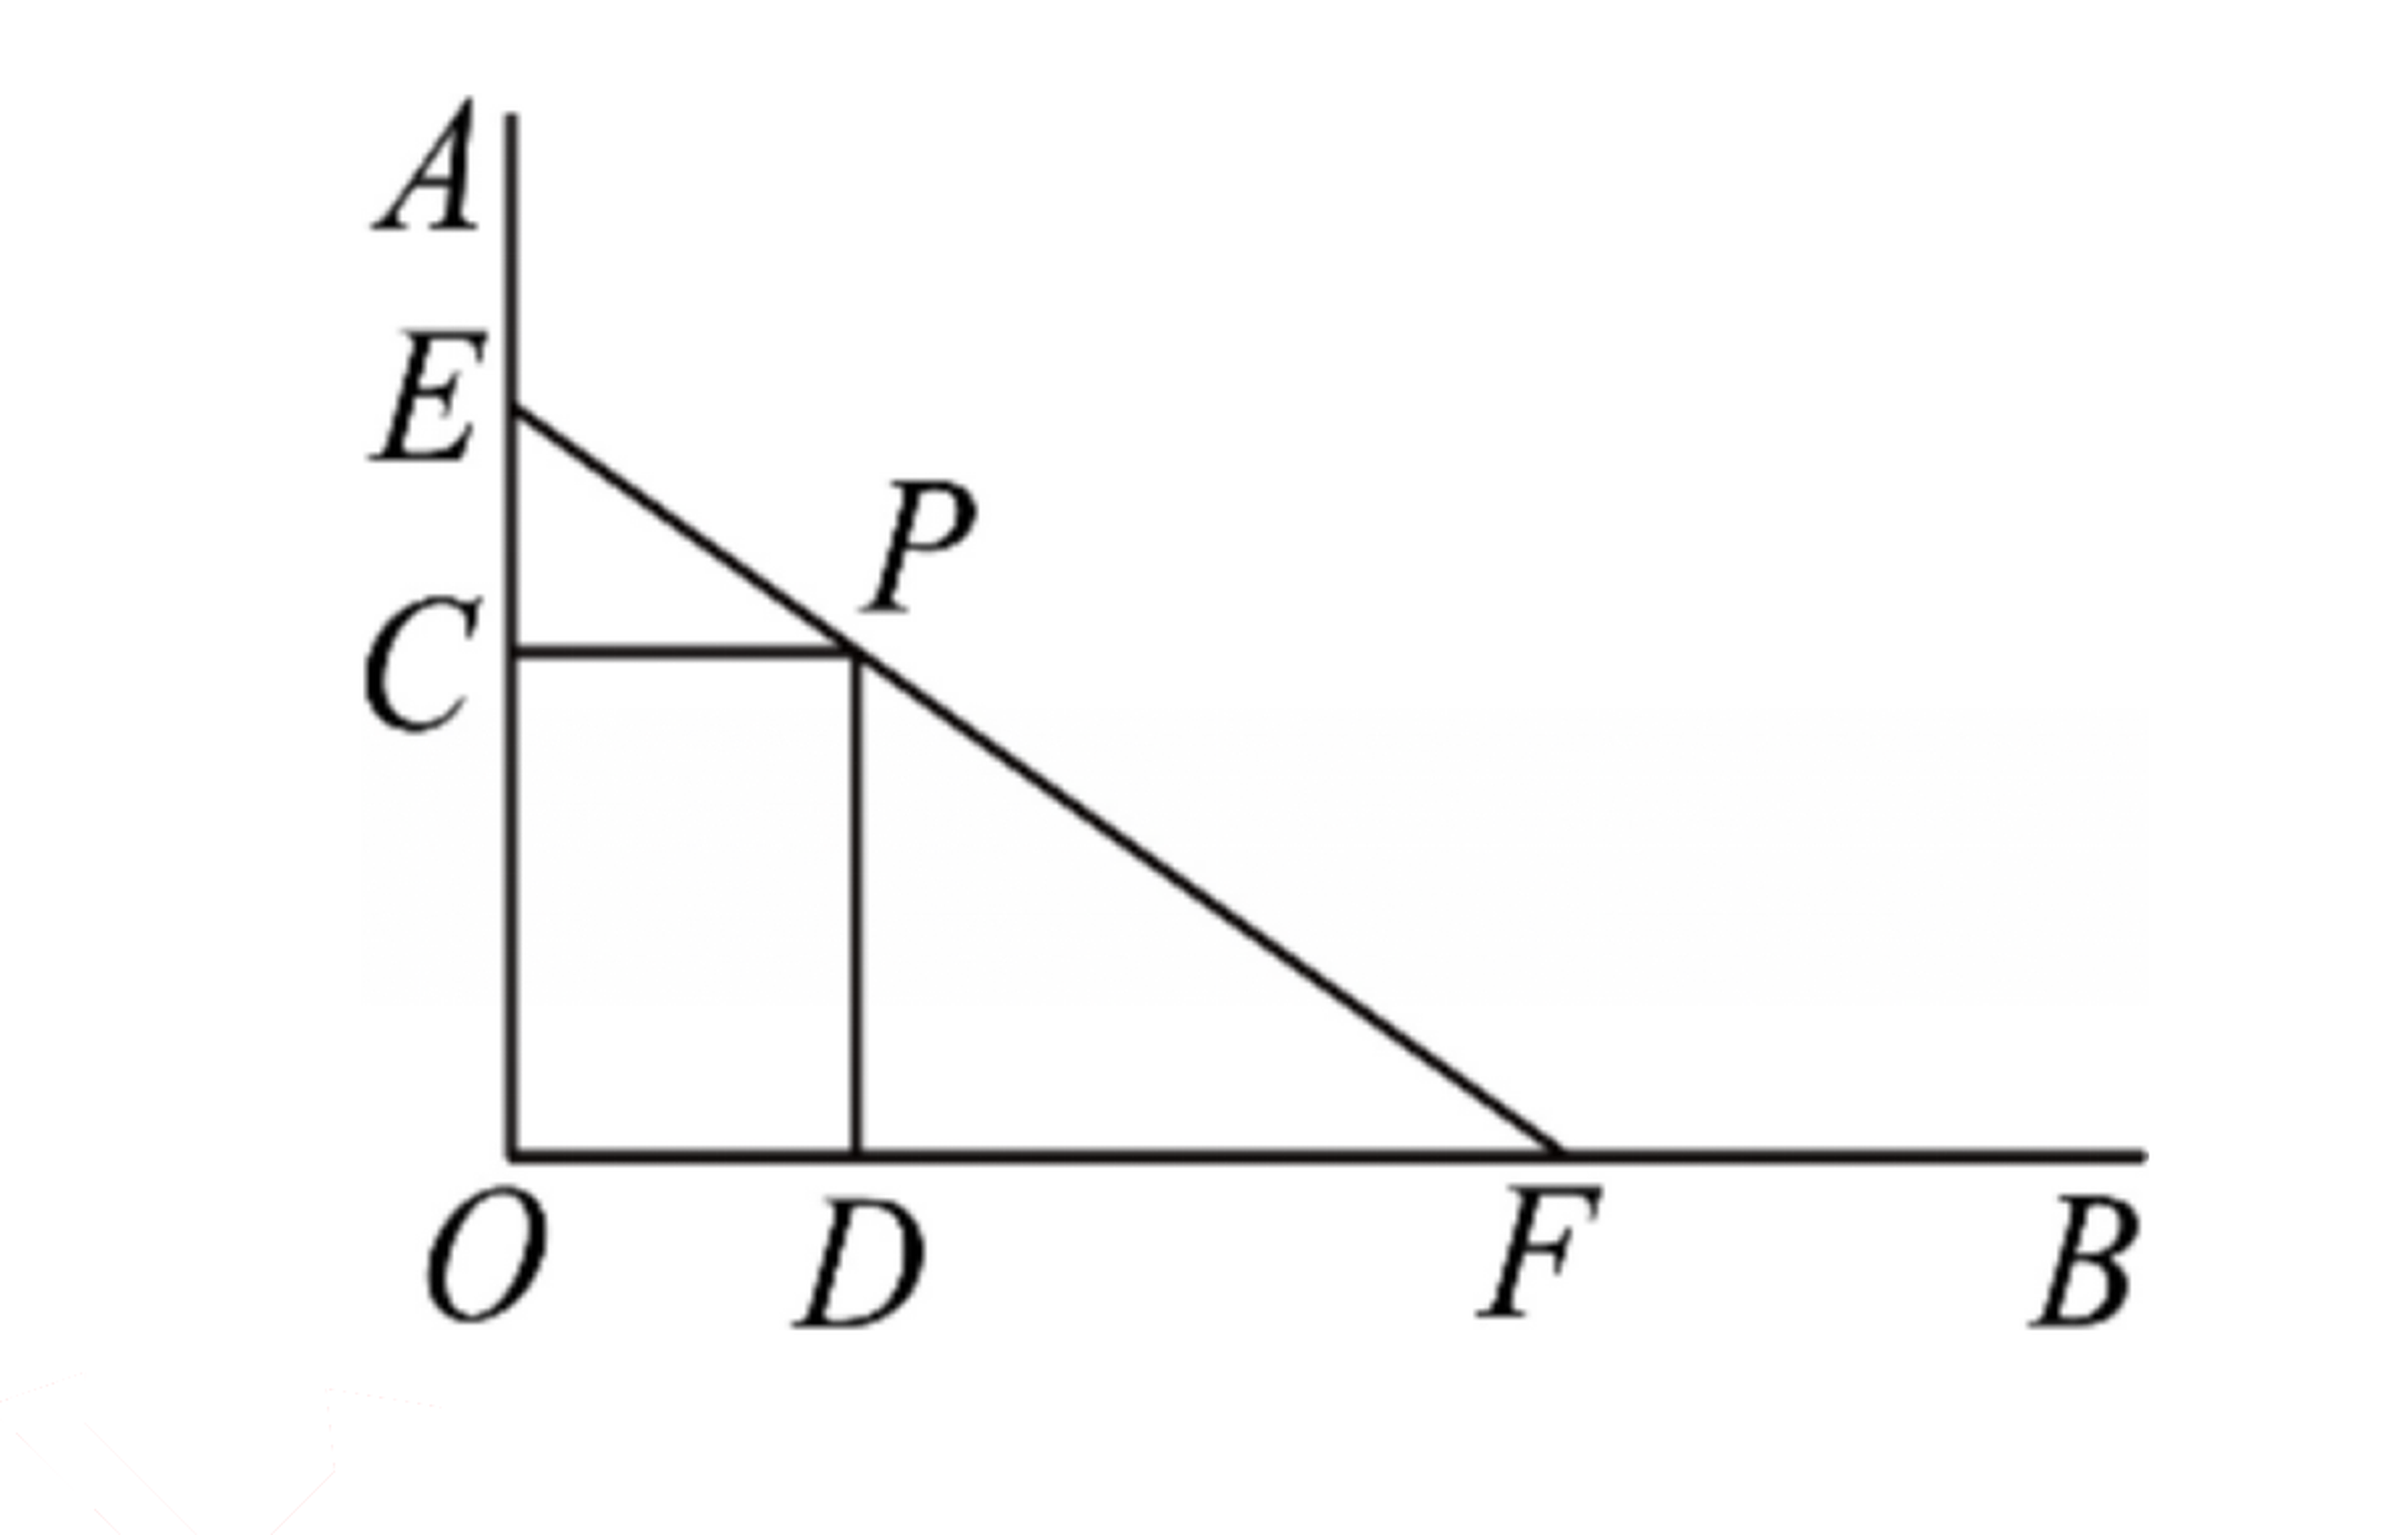
\includegraphics[width=0.32\textwidth]{figures/gao131_q19.png}
\end{center}

\ifanswer
\solbegin
\step{(1) 由题意得 $x\leq60$，}
\step{$\triangle PCE\sim\triangle FDP$，所以 $\dfrac{EC}{CP}=\dfrac{PD}{DF}$，即 $\dfrac{x}{25}=\dfrac{40}{DF}$，得 $DF=\dfrac{1000}{x}$m，}
\step{所以 $OF=OD+DF=\left(25+\dfrac{1000}{x}\right)$m，}
\step{所以 $25+\dfrac{1000}{x}\leq100$，解得 $x\geq\dfrac{40}{3}$；}
\step{综上，$\dfrac{40}{3}\leq x\leq60$；}
\step{(2) 由 $OE=OC+CE=(40+x)$m，}
\step{所以 $S=\dfrac12 OF\cdot OE=\dfrac12\left(25+\dfrac{1000}{x}\right)(40+x)$}
\step{$=\dfrac12\left(1000+25x+\dfrac{40000}{x}+1000\right)$m$^2$，}
\step{由基本不等式得 $S\geq\dfrac12\left(2000+2\sqrt{25x\cdot\dfrac{40000}{x}}\right)=2000$m$^2$，}
\step{当且仅当 $25x=\dfrac{40000}{x}$，即 $x=40$ 时取等号，}
\step{故 $EC=40$m 时，$S$ 取得最小值，为 $2000$m$^2$.}
\solend
\fi

\item 已知 $a\in\R$，函数 $y=ax^2+(3a+2)x+2a+3$.

(1) 当 $a=1$ 时，函数 $y=ax^2+(3a+2)x+2a+3$ 的图象与 $x$ 轴交于 $A(x_1,0)$，$B(x_2,0)$ 两点，求 $x_1^3+x_2^3$；

(2) 若关于 $x$ 的不等式 $ax^2+(3a+2)x+2a+3>2x$ 的解集为 $\R$，求实数 $a$ 的取值范围；

(3) 求关于 $x$ 的不等式 $y\geq1$ 的解集.

\ifanswer
\solbegin
\step{(1) 函数 $y=ax^2+(3a+2)x+2a+3$，当 $a=1$ 时，$y=x^2+5x+5$，}
\step{因为 $y=x^2+5x+5$ 的图象与 $x$ 轴交于 $A(x_1,0)$，$B(x_2,0)$ 两点，}
\step{即 $x^2+5x+5=0$ 的两个根为 $x_1$、$x_2$，}
\step{由根与系数的关系得 $x_1+x_2=-5$，$x_1x_2=5$，}
\step{所以 $x_1^2+x_2^2=(x_1+x_2)^2-2x_1x_2=25-10=15$，}
\step{所以 $x_1^3+x_2^3=(x_1+x_2)(x_1^2+x_2^2-x_1x_2)=-5\times(15-5)=-50$；}
\step{(2) 不等式 $ax^2+(3a+2)x+2a+3>2x$ 恒成立，得 $ax^2+3ax+2a+3>0$.}
\step{当 $a=0$ 时，$3>0$，恒成立，符合题意；}
\step{当 $a\neq0$ 时，若 $a<0$，二次函数 $ax^2+3ax+2a+3$ 开口向下，}
\step{一定存在小于零的部分，故不满足题意；}
\step{当 $a>0$ 时，若使 $ax^2+3ax+2a+3>0$ 恒成立，}
\step{只需 $\Delta=(3a)^2-4\times a\times(2a+3)=a^2-12a<0$，解得 $0<a<12$，}
\step{综上所述，$a$ 的取值范围为 $0\leq a<12$.}
\step{(3) 由 $y\geq1$，得 $ax^2+(3a+2)x+2a+3\geq1$，}
\step{即 $ax^2+(3a+2)x+2a+2\geq0$，即 $(ax+2a+2)(x+1)\geq0$，}
\step{当 $a=0$ 时，$2x+2\geq0$，解得 $x\geq-1$，}
\step{当 $a\neq0$ 时，}
\step{方程 $ax^2+(3a+2)x+2a+2=0$ 即为 $(x+1)(ax+2a+2)=0$，}
\step{解得 $x=-1$ 或 $x=-2-\dfrac2a$，令 $-1=-2-\dfrac2a$，即 $a=-2$，}
\step{当 $a>0$ 时，$-2-\dfrac2a<-1$，}
\step{不等式 $ax^2+(3a+2)x+2a+2\geq0$ 即为 $\left(x+\dfrac{2a+2}a\right)(x+1)\geq0$，}
\step{解得 $x\leq-2-\dfrac2a$ 或 $x\geq-1$；}
\step{当 $a<0$ 时，当 $-2-\dfrac2a<-1$，即 $a<-2$ 时，}
\step{不等式 $ax^2+(3a+2)x+2a+2\geq0$，即为 $\left(x+\dfrac{2a+2}a\right)(x+1)\leq0$，}
\step{解得 $-2-\dfrac2a\leq x\leq-1$；}
\step{当 $-2-\dfrac2a=-1$，即 $a=-2$，}
\step{不等式 $ax^2+(3a+2)x+2a+2\geq0$ 即为 $-2x^2-4x-2\geq0$，解得 $x=-1$，}
\step{当 $-2-\dfrac2a>-1$，即 $-2<a<0$ 时，}
\step{不等式 $ax^2+(3a+2)x+2a+2\geq0$ 即为 $\left(x+\dfrac{2a+2}a\right)(x+1)\leq0$，}
\step{解得 $-1\leq x\leq-2-\dfrac2a$，}
\step{综上所述，当 $a=0$ 时，解集为 $\{x\mid x\geq-1\}$；}
\step{当 $a>0$ 时，解集为 $\{x\mid x\leq-2-\dfrac2a$ 或 $x\geq-1\}$；}
\step{当 $a<-2$ 时，解集为 $\{x\mid -2-\dfrac2a\leq x\leq-1\}$；}
\step{当 $a=-2$ 时，解集为 $\{x\mid x=-1\}$；}
\step{当 $-2<a<0$ 时，解集为 $\{x\mid -1\leq x\leq-2-\dfrac2a\}$.}
\solend
\fi

\item 仔细阅读以下材料：【已知 $a$、$b\in(0,+\infty)$，$a+b=1$，求 $y=\dfrac1a+\dfrac2b$ 的最小值.

$y=\dfrac1a+\dfrac2b=\left(\dfrac1a+\dfrac2b\right)(a+b)=\dfrac ba+\dfrac{2a}b+3\geq3+2\sqrt2$，当且仅当 $\dfrac ba=\dfrac{2a}b$，即 $a=\sqrt2-1$，$b=2-\sqrt2$ 时取得等号，则 $y=\dfrac1a+\dfrac2b$ 的最小值为 $3+2\sqrt2$.

另 $y=\dfrac1a+\dfrac2b=\dfrac{a+b}a+\dfrac{2(a+b)}b=\dfrac ba+\dfrac{2a}b+3\geq3+2\sqrt2$，当且仅当 $\dfrac ba=\dfrac{2a}b$，即 $a=\sqrt2-1$，$b=2-\sqrt2$ 时取得等号，则 $y=\dfrac1a+\dfrac2b$ 的最小值为 $3+2\sqrt2$.】参考上述解法，求解下列问题.

(1) 若正实数 $x$、$y$ 满足 $x+y=1$，求 $\dfrac2x+\dfrac3y$ 的最小值；

(2) 已知 $x\in\left(0,\dfrac12\right)$，求 $t=\dfrac1x+\dfrac8{1-2x}$ 的最小值，并写出此时 $x$ 的值；

(3) 已知 $a$、$b\in(0,+\infty)$，$a+2b=1$，求 $p=\dfrac1{3a+4b}+\dfrac1{a+3b}$ 的最小值.

\ifanswer
\solbegin
\step{(1) 因为 $x>0,y>0$，且 $x+y=1$，}
\step{所以 $\dfrac2x+\dfrac3y=\left(\dfrac2x+\dfrac3y\right)(x+y)=2+\dfrac{2y}x+\dfrac{3x}y+3=5+\dfrac{2y}x+\dfrac{3x}y$，}
\step{由基本不等式得 $\dfrac{2y}x+\dfrac{3x}y\geq2\sqrt{\dfrac{2y}x\cdot\dfrac{3x}y}=2\sqrt6$，}
\step{当且仅当 $\dfrac{2y}x=\dfrac{3x}y$，即 $2y^2=3x^2$ 时，等号成立，}
\step{又因为 $x>0,y>0$ 且 $x+y=1$，此时 $x=\sqrt6-2,y=3-\sqrt6$，}
\step{所以 $\dfrac2x+\dfrac3y\geq5+2\sqrt6$，故 $\dfrac2x+\dfrac3y$ 的最小值为 $5+2\sqrt6$.}
\step{(2) 由 $0<x<\dfrac12$，则 $t=\dfrac1x+\dfrac8{1-2x}=\dfrac{2(1-2x+2x)}{2x}+\dfrac{8(1-2x+2x)}{1-2x}$}
\step{$=10+\dfrac{2\cdot(1-2x)}{2x}+\dfrac{8\cdot2x}{1-2x}\geq10+2\sqrt{\dfrac{2\cdot(1-2x)}{2x}\cdot\dfrac{8\cdot2x}{1-2x}}=18$，}
\step{当且仅当 $\dfrac{2\cdot(1-2x)}{2x}=\dfrac{8\cdot2x}{1-2x}$，即 $x=\dfrac16$ 时等号成立；}
\step{(3) 由 $a$、$b>0$，$a+2b=1$，则 $a=1-2b>0$，即 $0<b<\dfrac12$，}
\step{所以 $p=\dfrac1{3a+4b}+\dfrac1{a+3b}=\dfrac1{3a+6b-2b}+\dfrac1{a+2b+b}=\dfrac1{3-2b}+\dfrac1{1+b}$}
\step{$=\dfrac1{3-2b}+\dfrac2{2+2b}$，显然 $3-2b$、$2+2b>0$，}
\step{所以 $p=\dfrac15\cdot(3-2b+2+2b)\cdot\left(\dfrac1{3-2b}+\dfrac2{2+2b}\right)=\dfrac15\left[3+\dfrac{2+2b}{3-2b}+\dfrac{2(3-2b)}{2+2b}\right]$}
\step{$\geq\dfrac15\left[3+2\sqrt{\dfrac{2+2b}{3-2b}\cdot\dfrac{2(3-2b)}{2+2b}}\right]=\dfrac{3+2\sqrt2}5$，}
\step{当且仅当 $\dfrac{2+2b}{3-2b}=\dfrac{2(3-2b)}{2+2b}$，}
\step{即 $b=\dfrac{8-5\sqrt2}2$，$a=5\sqrt2-7$ 时等号成立.}
\solend
\fi

\end{enumerate}

\end{document}
"
% 紧凑版：xelatex "\def\iscompact{1}% 高一131_六十中学_期中.tex
%   —— 高一上数学"2026-2027 年六十中学高一上期中"（试卷版/答案版）
% 试卷版：xelatex 高一131_六十中学_期中.tex
% 答案版：xelatex "\def\isanswer{1}% 高一131_六十中学_期中.tex
%   —— 高一上数学"2026-2027 年六十中学高一上期中"（试卷版/答案版）
% 试卷版：xelatex 高一131_六十中学_期中.tex
% 答案版：xelatex "\def\isanswer{1}% 高一131_六十中学_期中.tex
%   —— 高一上数学"2026-2027 年六十中学高一上期中"（试卷版/答案版）
% 试卷版：xelatex 高一131_六十中学_期中.tex
% 答案版：xelatex "\def\isanswer{1}\input{高一131_六十中学_期中.tex}"
% 紧凑版：xelatex "\def\iscompact{1}\input{高一131_六十中学_期中.tex}"
%
% 原始材料：微信公众号"魔都数学加油站"文章，作者破晓，2026-11-13 18:18 发布；
% 连载"27学年高一131"，原文标题"27学年高一131——2026-2027年上海市六十中学高一上期中"；
% 原文链接：https://mp.weixin.qq.com/s/Nrbp3Uvt-sOGnOp4MEHemA。
% 正文为 11 张 PNG 页（01—05、09—11 为 2560x3620，06—08 为 4762x6735），
% 题目下印有【解析】或【答案】，为讲评版。题目、解析均据原图转录；
% 卷面粉红色水印"魔都数学加油站"及公众号页脚未录入。全卷仅第 19 题有 1 幅插图
% （矩形 OCPD 与小路 EF 的示意图），取 07.png 截图去水印。
%
% 卷首标题：原卷印作"2026-2027 年六十中学高一上期中"（公众号标题中的"上海市"
% 卷面标题行没有，本稿照卷面），年份区间按全稿惯例排 en dash；原卷未印副标题，
% 本卷为期中卷、跨集合与常用逻辑用语／不等式／函数三章，按题目内容标为
% "集合与常用逻辑用语、不等式、函数"（与 125／126／128／129 同期中卷口径相同）：
% 集合与逻辑见 Q3、Q4、Q7、Q13、Q17，不等式见 Q8、Q10、Q12、Q14、Q15、Q16、Q19、
% Q20、Q21，函数（指数／对数／幂函数、基本不等式应用）见 Q5、Q6、Q9、Q11、Q18、Q21。
%
% 题号体例：本卷共 19 题——一、填空题 3—12（10 题）、二、选择题 13—16（4 题）、
% 三、解答题 17—21（5 题）。三节分别 \setcounter{enumi}{2}／{12}／{16}。
%
% 与原卷的排版差异：
%   ① 原文从第 3 题起，本稿保留原题号（见上"题号体例"）；
%   ② 原卷每题下直接印【解析】／【答案】，本稿按全稿惯例置于答案版；第 3、4 题只印
%      【答案】，另提 \ans{}；第 13—16 题答案在解析末句"故选 …"，题干括号内留空、
%      不另提 \ans{}；其余各题印【解析】、无独立答案段；
%   ③ 原卷未印副标题，本稿按"知识模块"口径补出；
%   ④ 原卷填空横线按全稿惯例排为 \blankline[4.4em]；选择题括号排 \mbox{（\quad）}、
%      选项段前按惯例加 \keepwithprev；解答题不留作答区（原卷为讲评版，与 109—129 同）；
%   ⑤ 原卷数集排斜体 $R$／$N$，按全稿惯例改 \R／\N；绝对值排 \lvert…\rvert，
%      集合描述竖线排 \mid；不等号按全稿惯例排 \leqslant／\geqslant；
%   ⑥ 子题标号 (1)(2)(3) 原卷用半角括号，照录；圈数字 ①② 照录；
%   ⑦ 原卷第 19 题插图浮排在第 07 页题干右侧，本稿按体例就近置于题干"如图"之后
%      （居中 \includegraphics），图取原卷 07 页截图去水印；题前按惯例加
%      \needvspace{7cm} 守卫（照 高一120／127／129 成例），保证"题干 + 图"整块不被页边界切开；
%   ⑧ 原卷 Q9 题干跨 01—02 页、Q15 解析跨 03—04 页、Q16 材料跨 04—05 页、
%      Q17 题干跨 05—06 页、Q20 解析跨 08—09 页、Q21 解析跨 09—11 页，
%      本稿按题合并连续排版；末页第 11 页为 Q21 (3) 解析的续尾，按实际印刷行单列。
%   ⑨ 第 16 题材料英文括注原卷印作 (Cauchy – SchwarzInequality)（长横、Schwarz 与
%      Inequality 斜体连排无空格），本稿按全稿英文专名惯例排 \emph{(Cauchy-Schwarz Inequality)}；
%      第 15 题解析 B、D 两行原卷各印一步含 \lg m 的换底繁分数（2026-11-13 回原图核对补回，
%      本稿初转曾顺手去重跳过该步）。
%
% 判别式字形：第 20 题 (2) 解析 $\Delta=(3a)^2-4\times a\times(2a+3)=a^2-12a<0$
%   原卷排三角形（等腰、高；回 08.png 放大核对），照录 \Delta；全卷判别式仅此一处
%   （\triangle 另作第 19 题「$\triangle PCE\sim\triangle FDP$」的几何三角形记号）。
%
% 子集符号：第 17 题 (2) 解析 $P\subseteq Q$ 印带下划线，照录 \subseteq；
%   全卷未出现单线 \subset。
%
% 原卷存疑照录：
%   第 11 题解析末两式作 $\dfrac{2+m+\frac1n}{2n+2}=\dfrac{2n+mn+1}{2n+2}$，而第三式
%     分母 $\log_3 9+\log_3 2+\log_3 2=2+\frac2n$，与前一分母 $2n+2$ 不等，照录；
%   第 16 题材料 ①"对于所有实数 $x$ 和 $y$，有 $(a^2+b^2)(c^2+d^2)\geq(ac+bd)^2$"
%     句首用 $x$、$y$ 而式中用 $a$、$b$、$c$、$d$，照录；
%   第 20 题题干 (2) 作"解集为 $\R$"、解析 (2) 作"恒成立"，措辞不同，照录；
%   第 21 题材料把同一道题用两种解法连印两遍（"另 $y=\frac1a+\frac2b=\dots$"），照录；
%   第 21 题 (3) 解析末句"即 $b=\frac{8-5\sqrt2}{2}$，$a=5\sqrt2-7$ 时等号成立"
%     未另写"故最小值为 $\frac{3+2\sqrt2}{5}$"，照录；
%   第 12 题解析"所以 $e^a+e^b>e^c, a+b>c$"、第 8 题解析"$a>0$，$b>0$"、
%     第 18 题 (2)"$4x^2-4x+1<x^2+4x+4$，解得 $-\frac13<x<3$"等处数学式内
%     半角逗号，照录；
%   第 15 题解析用 $\lg$ 记常用对数（$\lg m$、$\lg 3$、$\lg 5$、$\lg 15$），照录。
%
% 行数复核：逐题数 \step 条数，合计 119 条（Q3：0；Q4：0；Q5：1；Q6：1；Q7：2；
% Q8：2；Q9：1；Q10：1；Q11：2；Q12：6；Q13：2；Q14：3；Q15：14；Q16：10；
% Q17：4；Q18：8；Q19：11；Q20：35；Q21：16），与原卷印刷行逐题相等
% （cases 块作一个印刷行计）。第 3、4 题只印【答案】，提 \ans{}，不计入 \step 账；
% 四道选择题答案均在解析末句，括号内留空、不另提 \ans{}。
%
\documentclass[a4paper,11pt]{article}
\usepackage{common}

\begin{document}

\examtitlest[3]{2026--2027 年六十中学高一上期中}{集合与常用逻辑用语、不等式、函数}

\bigsec{一、填空题}

\begin{enumerate}
\setcounter{enumi}{2}

\item 已知集合 $A=(0,4),B=[2,5]$，则 $A\cup B=$\blankline[4.4em].

\ifanswer
\ans{$(0,5]$}
\fi

\item 陈述句“$x=2$ 或 $y=3$”的否定形式为\blankline[4.4em].

\ifanswer
\ans{$x\neq2$ 且 $y\neq3$}
\fi

\item 函数 $y=a^{x-2}+15(a>0$ 且 $a\neq1)$ 的图象恒过定点的坐标为\blankline[4.4em].

\ifanswer
\solbegin
\step{函数 $y=a^{x-2}+15$ 的图象恒过定点 $A(2,16)$.}
\solend
\fi

\item 用有理数指数幂的形式来化简：$\dfrac{\sqrt{a\cdot\sqrt[3]{a^4}}}{\left(a^{\frac13}\right)^2}=$\blankline[4.4em].

\ifanswer
\solbegin
\step{原式 $=\dfrac{\sqrt{a\cdot a^{\frac43}}}{a^{\frac23}}=\dfrac{\sqrt{a^{\frac73}}}{a^{\frac23}}=\dfrac{a^{\frac76}}{a^{\frac23}}=a^{\frac76-\frac23}=a^{\frac12}(a>0)$.}
\solend
\fi

\item 已知集合 $A=\left\{x\mid \dfrac6{6-x}\in\N\text{ 且 }x\in\N\right\}$，则用列举法表示集合 $A=$\blankline[4.4em].

\ifanswer
\solbegin
\step{当 $x=0$ 时，$\dfrac6{6-0}=1\in\N$，当 $x=3$ 时，$\dfrac6{6-3}=2\in\N$，}
\step{当 $x=4$ 时，$\dfrac6{6-4}=3\in\N$，当 $x=5$ 时，$\dfrac6{6-5}=6\in\N$，故 $A=\{0,3,4,5\}$.}
\solend
\fi

\item 已知 $a>0$，$b>0$，且 $ab=\dfrac12$，则 $\dfrac1a+\dfrac8b$ 的最小值是\blankline[4.4em].

\ifanswer
\solbegin
\step{$a>0$，$b>0$，且 $ab=\dfrac12$，则 $\dfrac1a+\dfrac8b\geq2\sqrt{\dfrac8{ab}}=8$，}
\step{当且仅当 $\dfrac1a=\dfrac8b$，即 $a=\dfrac14,b=2$ 时取等号，故最小值为 $8$.}
\solend
\fi

\item 心理学家有时用函数 $L(t)=A(1-e^{-kt})$ 测定在时间 $t$（单位：$min$）内能够记忆的量 $L$，其中 $A$ 表示需要记忆的量，$k$ 表示记忆率. 假设一个学生需要记忆的量为 $200$ 个单词，此时 $L$ 表示在时间 $t$ 内该生能够记忆的单词个数. 已知该生在 $5min$ 内能够记忆 $20$ 个单词，则 $k$ 的值约为\blankline[4.4em]（结果保留四位小数）.

\ifanswer
\solbegin
\step{由题意得 $200(1-e^{-5k})=20$，所以 $e^{-5k}=0.9$，解得 $k\approx0.0211$.}
\solend
\fi

\item 设 $x\in\R$，方程 $\lvert 3x-2\rvert+\lvert 1-x\rvert=\lvert 2x-1\rvert$ 的解集是\blankline[4.4em].

\ifanswer
\solbegin
\step{由三角不等式得 $(3x-2)(1-x)\geq0$，故解集是 $\left[\dfrac23,1\right]$.}
\solend
\fi

\item 已知 $3^m=5$，$n=\log_2 3$，则 $\log_{36}90$ 可用 $m$、$n$ 表示为\blankline[4.4em].

\ifanswer
\solbegin
\step{由 $3^m=5$，又 $n=\log_2 3$，得 $m=\log_3 5$，$\log_3 2=\dfrac{\log_2 2}{\log_2 3}=\dfrac1n$，}
\step{所以 $\log_{36}90=\dfrac{\log_3 90}{\log_3 36}=\dfrac{\log_3 9+\log_3 2+\log_3 5}{\log_3 9+\log_3 2+\log_3 2}=\dfrac{2+m+\frac1n}{2n+2}=\dfrac{2n+mn+1}{2n+2}$.}
\solend
\fi

\item 若定义域为 $I=(0,m]$ 的函数 $f(x)=e^x$ 满足：对任意能构成三角形三边长的实数 $a$、$b$、$c\in I$，均有 $f(a)$、$f(b)$、$f(c)$ 也能构成三角形三边长，则 $m$ 的最大值为\blankline[4.4em].

\ifanswer
\solbegin
\step{$f(x)=e^x$ 在 $I=(0,m]$ 上严格增，所以 $f(x)\in(1,e^m]$，不妨设 $0<a\leq b\leq c$，}
\step{因为对任意能构成三角形三边长的实数 $a,b,c\in I$，均有 $f(a)$，$f(b)$，$f(c)$}
\step{也能构成三角形三边长，所以 $e^a+e^b>e^c, a+b>c$，}
\step{因为 $e^a+e^b\geq2\sqrt{e^ae^b}=2\sqrt{e^{a+b}}>e^c$，所以 $4e^{a+b}>e^{2c}$，}
\step{因为对任意 $a,b,c\in I$ 都成立，所以 $4e^c\geq e^{2c}$，所以 $e^c\leq4$，所以 $c\leq\ln4$，}
\step{所以 $m\leq\ln4$，所以 $m$ 的最大值为 $\ln4$.}
\solend
\fi

\end{enumerate}

\bigsec{二、选择题}

\begin{enumerate}
\setcounter{enumi}{12}

\item 已知 $m,n$ 是非零自然数，命题 $\alpha:mn$ 是奇数，命题 $\beta:m$ 或 $n$ 是奇数，则 $\alpha$ 是 $\beta$ 的\mbox{（\quad）}

\keepwithprev
A. 充分非必要条件\qquad\qquad B. 必要非充分条件

C. 充要条件\qquad\qquad D. 既非充分又非必要条件

\ifanswer
\solbegin
\step{$mn$ 是奇数 $\Leftrightarrow$ $m$、$n$ 都是奇数，所以 $\alpha$ 能推出 $\beta$，充分性成立，}
\step{但 $\beta$ 推不出 $\alpha$，必要性不成立，所以 $\alpha$ 是 $\beta$ 的充分非必要条件. 故选 $A$.}
\solend
\fi

\item 关于 $x$ 的不等式 $x^2-mx+n+5\leq0$ 的解集是 $[1,8]$，那么 $\log_m n=$\mbox{（\quad）}

\keepwithprev
A. $\dfrac13$\qquad\qquad B. $-3$\qquad\qquad C. $-2$\qquad\qquad D. $\dfrac12$

\ifanswer
\solbegin
\step{由题意得 $x^2-mx+n+5=0$ 的解为 $1$，$8$，}
\step{由根与系数的关系得 $\begin{cases}1+8=m\\1\times8=n+5\end{cases}$，解得 $m=9$，$n=3$，}
\step{所以 $\log_m n=\log_9 3=\dfrac12\log_3 3=\dfrac12$. 故选 $D$.}
\solend
\fi

\item 已知正实数 $x$、$y$、$z$ 满足 $3^x=5^y=15^z$，则下列说法中不正确的是\mbox{（\quad）}

\keepwithprev
A. $\dfrac1x+\dfrac1y=\dfrac1z$\qquad\qquad B. $x+y>2z$\qquad\qquad C. $3x>5y>15z$\qquad\qquad D. $x\cdot y>4z^2$

\ifanswer
\solbegin
\step{已知正实数 $x$、$y$、$z$，则设 $3^x=5^y=15^z=m>1$，}
\step{所以 $x=\log_3 m$，$y=\log_5 m$，$z=\log_{15} m$，}
\step{对于 $A$，$\dfrac1x+\dfrac1y=\dfrac1{\log_3 m}+\dfrac1{\log_5 m}=\log_m 3+\log_m 5=\log_m 15=\dfrac1z$，故 $A$ 正确；}
\step{对于 $B$，因为 $\dfrac{x+y}{z}=\dfrac{x}{z}+\dfrac{y}{z}=\dfrac{\log_3 m}{\log_{15} m}+\dfrac{\log_5 m}{\log_{15} m}=\dfrac{\dfrac{\lg m}{\lg3}}{\dfrac{\lg m}{\lg15}}+\dfrac{\dfrac{\lg m}{\lg5}}{\dfrac{\lg m}{\lg15}}=\dfrac{\lg15}{\lg3}+\dfrac{\lg15}{\lg5}$，}
\step{$=\dfrac{\lg3+\lg5}{\lg3}+\dfrac{\lg3+\lg5}{\lg5}=2+\dfrac{\lg5}{\lg3}+\dfrac{\lg3}{\lg5}=2+\log_3 5+\log_5 3$，}
\step{又 $\log_3 5>0$，$\log_5 3>0$，所以 $2+\log_3 5+\log_5 3>2$，}
\step{所以 $\dfrac{x+y}{z}>2$，即 $x+y>2z$，故 $B$ 正确；}
\step{对于 $C$，因为 $\dfrac5x=5\log_m 3=\log_m 243$，$\dfrac3y=3\log_m 5=\log_m 125$，}
\step{所以 $\dfrac5x>\dfrac3y$，即 $3x<5y$，故 $C$ 错误；}
\step{对于 $D$，$\dfrac{xy}{z^2}=\dfrac{x}{z}\cdot\dfrac{y}{z}=\dfrac{\log_3 m}{\log_{15} m}\cdot\dfrac{\log_5 m}{\log_{15} m}=\dfrac{\dfrac{\lg m}{\lg3}}{\dfrac{\lg m}{\lg15}}\cdot\dfrac{\dfrac{\lg m}{\lg5}}{\dfrac{\lg m}{\lg15}}=\dfrac{\lg15}{\lg3}\cdot\dfrac{\lg15}{\lg5}$}
\step{$=\dfrac{\lg3+\lg5}{\lg3}\cdot\dfrac{\lg3+\lg5}{\lg5}=\left(1+\dfrac{\lg5}{\lg3}\right)\left(1+\dfrac{\lg3}{\lg5}\right)=2+\dfrac{\lg5}{\lg3}+\dfrac{\lg3}{\lg5}$}
\step{$\geq2+2\sqrt{\dfrac{\lg5}{\lg3}\cdot\dfrac{\lg3}{\lg5}}=2+2=4$，又 $\lg3\neq\lg5$，故等号不成立，}
\step{所以 $\dfrac{xy}{z^2}>4$，即 $xy>4z^2$，故 $D$ 正确.}
\step{故选 $C$.}
\solend
\fi

\item 柯西不等式 \emph{(Cauchy-Schwarz Inequality)} 是一种在数学和物理学中广泛使用的不等式，它是由法国数学家奥古斯丁$\cdot$路易$\cdot$柯西提出的，柯西不等式可以用于证明其他不等式，也可以用于解决一些数学问题. 以下是柯西不等式的原始形式：

①对于所有实数 $x$ 和 $y$，有 $(a^2+b^2)(c^2+d^2)\geq(ac+bd)^2$.

②等式条件：当且仅当 $ad-bc=0$ 时，等号成立.

例：已知 $x+2y=2$，由柯西不等式 $(x^2+y^2)(1^2+2^2)\geq(x+2y)^2$，可得 $(x^2+y^2)_{min}=\dfrac45$.

现给出以下两个命题：

①若 $a^2+b^2=1$，则 $2a+3b$ 的最大值为 $\sqrt{13}$；

②若 $1<a<3$，则 $\sqrt{a-1}+\sqrt{6-2a}$ 的最大值为 $\sqrt6$；

则运用柯西不等式，判断以下正确的选项有\mbox{（\quad）}

\keepwithprev
A. ①为真命题；②为真命题\qquad\qquad B. ①为真命题；②为假命题

C. ①为假命题；②为真命题\qquad\qquad D. ①为假命题；②为假命题

\ifanswer
\solbegin
\step{由柯西不等式得 $(a^2+b^2)(2^2+3^2)\geq(2a+3b)^2$.}
\step{因为 $a^2+b^2=1$，所以 $(2^2+3^2)\geq(2a+3b)^2$，即 $13\geq(2a+3b)^2$，}
\step{所以 $-\sqrt{13}\leq2a+3b\leq\sqrt{13}$，则 $(2a+3b)_{max}=\sqrt{13}$，}
\step{当且仅当 $3a=2b$ 时取等号，故①正确.}
\step{令 $x=\sqrt{a-1}$，$y=\sqrt{3-a}$，则 $x^2+y^2=a-1+3-a=2$，}
\step{由柯西不等式得 $(\sqrt{a-1}+\sqrt{6-2a})^2=(\sqrt{a-1}+\sqrt2\cdot\sqrt{3-a})^2=(x+\sqrt2 y)^2$}
\step{$\leq[1^2+(\sqrt2)^2](x^2+y^2)$，}
\step{因为 $x^2+y^2=2$，所以 $(\sqrt{a-1}+\sqrt{6-2a})^2\leq6$，}
\step{当且仅当 $\sqrt{3-a}=\sqrt2\sqrt{a-1}$ 取等号，所以 $\sqrt{a-1}+\sqrt{6-2a}\leq\sqrt6$，故②正确.}
\step{故选 $A$.}
\solend
\fi

\end{enumerate}

\bigsec{三、解答题}

\begin{enumerate}
\setcounter{enumi}{16}

\item 已知集合 $P=\left\{x\mid \dfrac{3x-1}{x+2}<1\right\}$，集合 $Q=\{x\mid\lvert x-a\rvert\leq2\}$.

(1) 求集合 $P$；

(2) 若“$x\in P$”是“$x\in Q$”的充分非必要条件，求实数 $a$ 的取值范围.

\ifanswer
\solbegin
\step{(1) 集合 $P=\left\{x\mid \dfrac{3x-1}{x+2}<1\right\}$，得 $\dfrac{2x-3}{x+2}<0$，解得 $P=\left(-2,\dfrac32\right)$.}
\step{(2) 集合 $Q=\{x\mid\lvert x-a\rvert\leq2\}=\{x\mid a-2\leq x\leq2+a\}$，}
\step{由“$x\in P$”是“$x\in Q$”的充分非必要条件，得 $P\subseteq Q$，}
\step{得 $\begin{cases}-2\geq a-2\\\dfrac32\leq2+a\\a-2<2+a\end{cases}$，解得 $a\in\left[-\dfrac12,0\right]$.}
\solend
\fi

\item 已知幂函数 $f(x)=(m^2-4m+4)\cdot x^{2m-4}$ 在 $(-\infty,0)$ 上是严格减函数.

(1) 求函数 $y=f(x)$ 的解析式；

(2) 若 $f(1-2x)<f(x+2)$，求 $x$ 的取值范围.

\ifanswer
\solbegin
\step{(1) 由幂函数的定义得 $m^2-4m+4=1$，解得 $m=1$ 或 $3$，}
\step{当 $m=1$ 时，$f(x)=x^{-2}=\dfrac1{x^2}$，在 $(-\infty,0)$ 上严格增，不符合题意，}
\step{当 $m=3$ 时，$f(x)=x^2$，在 $(-\infty,0)$ 上严格减，符合题意，}
\step{所以 $f(x)=x^2$；}
\step{(2) 由函数 $f(x)=x^2$ 图象关于 $y$ 轴对称，且在 $[0,+\infty)$ 上严格增，}
\step{则 $f(1-2x)<f(x+2)$ 可化为 $\lvert1-2x\rvert<\lvert x+2\rvert$，}
\step{平方得 $4x^2-4x+1<x^2+4x+4$，解得 $-\dfrac13<x<3$，}
\step{所以 $x$ 的取值范围是 $\left(-\dfrac13,3\right)$.}
\solend
\fi

% 第 19 题是"题干 + 图"约 7cm 的一整块，守卫放在 \item 之前（放 \item 之后会失效）
\needvspace{7cm}
\item 如图，$OA$、$OB$ 是两条长度足够长的互相垂直的笔直小路，矩形 $OCPD$ 的顶点 $C$，$D$ 分别在 $OA$、$OB$ 上，且该矩形区域内种满了荷花. 为了让观赏者有更好的观赏体验，现计划经过点 $P$ 修一条小路 $EF$，其中点 $E$ 在小路 $OA$ 上，点 $F$ 在小路 $OB$ 上，并在 $\triangle OEF$ 区域内种满荷花. 已知 $OD=25m$，$OC=40m$，且小路 $EF$ 要完全位于一个以 $O$ 为顶点的，边长为 $100$ m 的正方形内部（包括边界）. 记 $\triangle OEF$ 的面积为 $S$m$^2$.

(1) 设 $EC=x\cdot m$，试用 $x$ 表示 $OF$，并求 $x$ 的取值范围.

(2) 当 $EC$ 的长度为多少时，$S$ 取得最小值？最小值是多少？

\begin{center}
% 图取原卷 07.png 截图去粉色水印，2.8× LANCZOS 放大
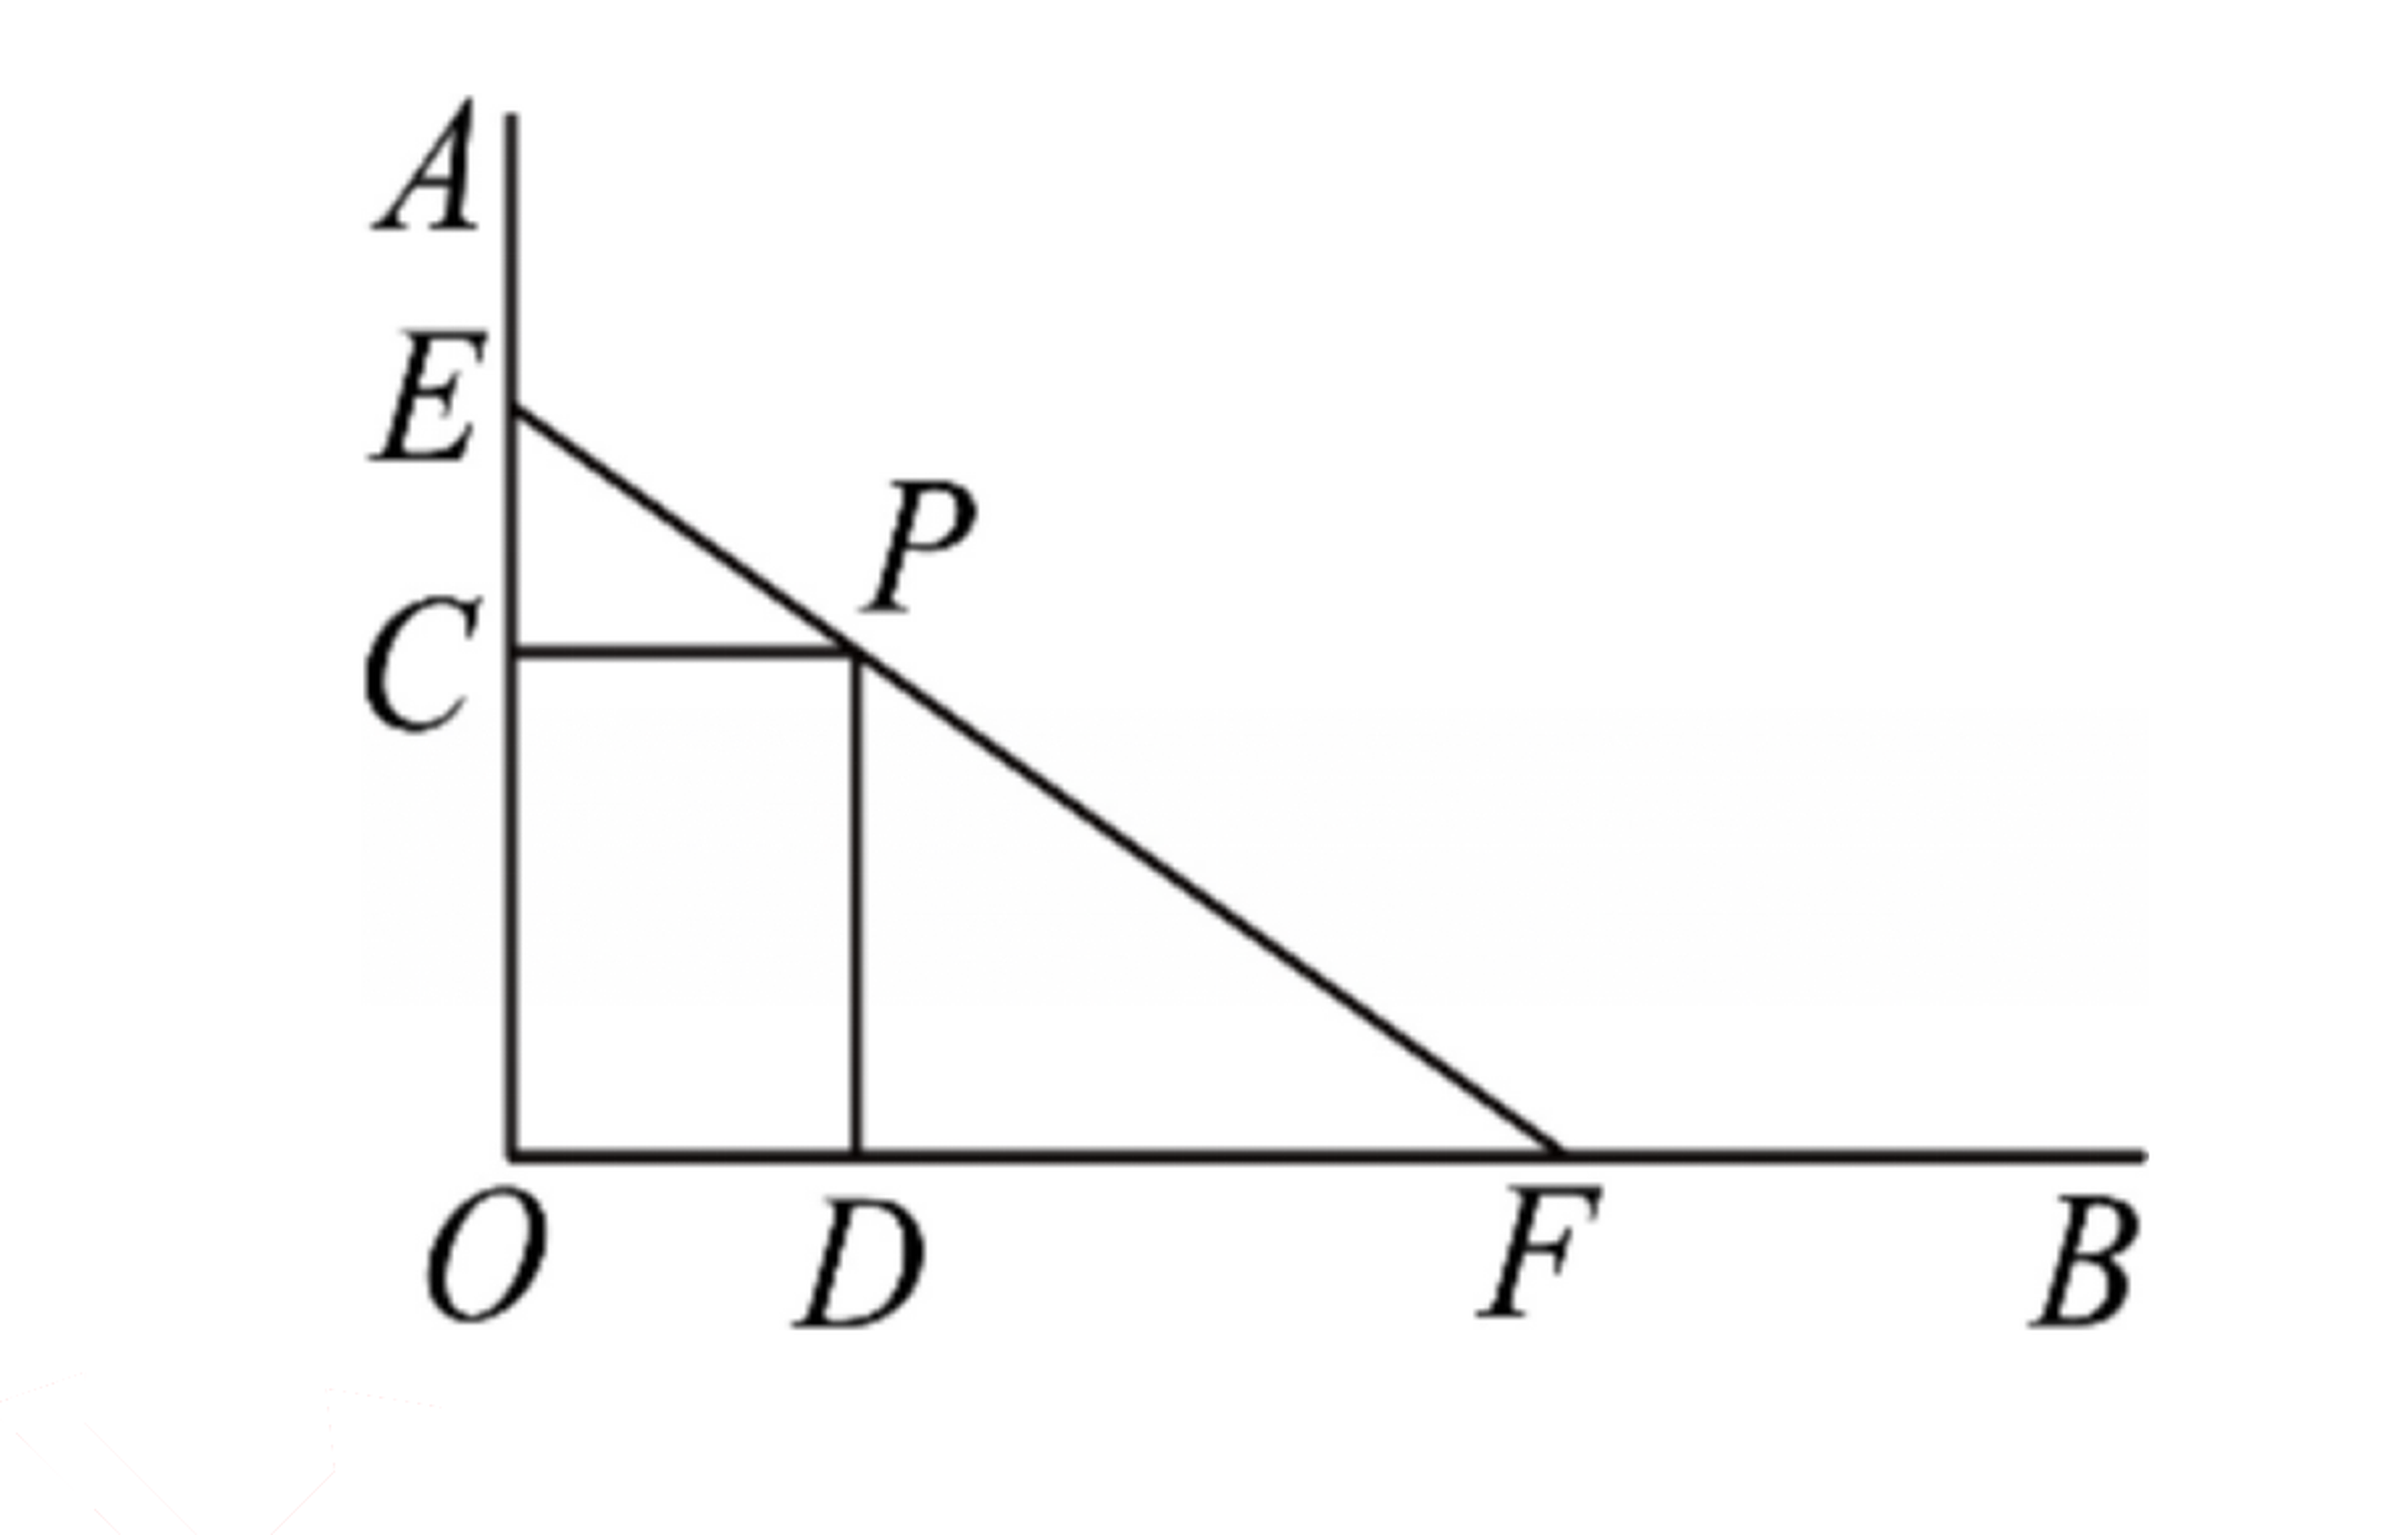
\includegraphics[width=0.32\textwidth]{figures/gao131_q19.png}
\end{center}

\ifanswer
\solbegin
\step{(1) 由题意得 $x\leq60$，}
\step{$\triangle PCE\sim\triangle FDP$，所以 $\dfrac{EC}{CP}=\dfrac{PD}{DF}$，即 $\dfrac{x}{25}=\dfrac{40}{DF}$，得 $DF=\dfrac{1000}{x}$m，}
\step{所以 $OF=OD+DF=\left(25+\dfrac{1000}{x}\right)$m，}
\step{所以 $25+\dfrac{1000}{x}\leq100$，解得 $x\geq\dfrac{40}{3}$；}
\step{综上，$\dfrac{40}{3}\leq x\leq60$；}
\step{(2) 由 $OE=OC+CE=(40+x)$m，}
\step{所以 $S=\dfrac12 OF\cdot OE=\dfrac12\left(25+\dfrac{1000}{x}\right)(40+x)$}
\step{$=\dfrac12\left(1000+25x+\dfrac{40000}{x}+1000\right)$m$^2$，}
\step{由基本不等式得 $S\geq\dfrac12\left(2000+2\sqrt{25x\cdot\dfrac{40000}{x}}\right)=2000$m$^2$，}
\step{当且仅当 $25x=\dfrac{40000}{x}$，即 $x=40$ 时取等号，}
\step{故 $EC=40$m 时，$S$ 取得最小值，为 $2000$m$^2$.}
\solend
\fi

\item 已知 $a\in\R$，函数 $y=ax^2+(3a+2)x+2a+3$.

(1) 当 $a=1$ 时，函数 $y=ax^2+(3a+2)x+2a+3$ 的图象与 $x$ 轴交于 $A(x_1,0)$，$B(x_2,0)$ 两点，求 $x_1^3+x_2^3$；

(2) 若关于 $x$ 的不等式 $ax^2+(3a+2)x+2a+3>2x$ 的解集为 $\R$，求实数 $a$ 的取值范围；

(3) 求关于 $x$ 的不等式 $y\geq1$ 的解集.

\ifanswer
\solbegin
\step{(1) 函数 $y=ax^2+(3a+2)x+2a+3$，当 $a=1$ 时，$y=x^2+5x+5$，}
\step{因为 $y=x^2+5x+5$ 的图象与 $x$ 轴交于 $A(x_1,0)$，$B(x_2,0)$ 两点，}
\step{即 $x^2+5x+5=0$ 的两个根为 $x_1$、$x_2$，}
\step{由根与系数的关系得 $x_1+x_2=-5$，$x_1x_2=5$，}
\step{所以 $x_1^2+x_2^2=(x_1+x_2)^2-2x_1x_2=25-10=15$，}
\step{所以 $x_1^3+x_2^3=(x_1+x_2)(x_1^2+x_2^2-x_1x_2)=-5\times(15-5)=-50$；}
\step{(2) 不等式 $ax^2+(3a+2)x+2a+3>2x$ 恒成立，得 $ax^2+3ax+2a+3>0$.}
\step{当 $a=0$ 时，$3>0$，恒成立，符合题意；}
\step{当 $a\neq0$ 时，若 $a<0$，二次函数 $ax^2+3ax+2a+3$ 开口向下，}
\step{一定存在小于零的部分，故不满足题意；}
\step{当 $a>0$ 时，若使 $ax^2+3ax+2a+3>0$ 恒成立，}
\step{只需 $\Delta=(3a)^2-4\times a\times(2a+3)=a^2-12a<0$，解得 $0<a<12$，}
\step{综上所述，$a$ 的取值范围为 $0\leq a<12$.}
\step{(3) 由 $y\geq1$，得 $ax^2+(3a+2)x+2a+3\geq1$，}
\step{即 $ax^2+(3a+2)x+2a+2\geq0$，即 $(ax+2a+2)(x+1)\geq0$，}
\step{当 $a=0$ 时，$2x+2\geq0$，解得 $x\geq-1$，}
\step{当 $a\neq0$ 时，}
\step{方程 $ax^2+(3a+2)x+2a+2=0$ 即为 $(x+1)(ax+2a+2)=0$，}
\step{解得 $x=-1$ 或 $x=-2-\dfrac2a$，令 $-1=-2-\dfrac2a$，即 $a=-2$，}
\step{当 $a>0$ 时，$-2-\dfrac2a<-1$，}
\step{不等式 $ax^2+(3a+2)x+2a+2\geq0$ 即为 $\left(x+\dfrac{2a+2}a\right)(x+1)\geq0$，}
\step{解得 $x\leq-2-\dfrac2a$ 或 $x\geq-1$；}
\step{当 $a<0$ 时，当 $-2-\dfrac2a<-1$，即 $a<-2$ 时，}
\step{不等式 $ax^2+(3a+2)x+2a+2\geq0$，即为 $\left(x+\dfrac{2a+2}a\right)(x+1)\leq0$，}
\step{解得 $-2-\dfrac2a\leq x\leq-1$；}
\step{当 $-2-\dfrac2a=-1$，即 $a=-2$，}
\step{不等式 $ax^2+(3a+2)x+2a+2\geq0$ 即为 $-2x^2-4x-2\geq0$，解得 $x=-1$，}
\step{当 $-2-\dfrac2a>-1$，即 $-2<a<0$ 时，}
\step{不等式 $ax^2+(3a+2)x+2a+2\geq0$ 即为 $\left(x+\dfrac{2a+2}a\right)(x+1)\leq0$，}
\step{解得 $-1\leq x\leq-2-\dfrac2a$，}
\step{综上所述，当 $a=0$ 时，解集为 $\{x\mid x\geq-1\}$；}
\step{当 $a>0$ 时，解集为 $\{x\mid x\leq-2-\dfrac2a$ 或 $x\geq-1\}$；}
\step{当 $a<-2$ 时，解集为 $\{x\mid -2-\dfrac2a\leq x\leq-1\}$；}
\step{当 $a=-2$ 时，解集为 $\{x\mid x=-1\}$；}
\step{当 $-2<a<0$ 时，解集为 $\{x\mid -1\leq x\leq-2-\dfrac2a\}$.}
\solend
\fi

\item 仔细阅读以下材料：【已知 $a$、$b\in(0,+\infty)$，$a+b=1$，求 $y=\dfrac1a+\dfrac2b$ 的最小值.

$y=\dfrac1a+\dfrac2b=\left(\dfrac1a+\dfrac2b\right)(a+b)=\dfrac ba+\dfrac{2a}b+3\geq3+2\sqrt2$，当且仅当 $\dfrac ba=\dfrac{2a}b$，即 $a=\sqrt2-1$，$b=2-\sqrt2$ 时取得等号，则 $y=\dfrac1a+\dfrac2b$ 的最小值为 $3+2\sqrt2$.

另 $y=\dfrac1a+\dfrac2b=\dfrac{a+b}a+\dfrac{2(a+b)}b=\dfrac ba+\dfrac{2a}b+3\geq3+2\sqrt2$，当且仅当 $\dfrac ba=\dfrac{2a}b$，即 $a=\sqrt2-1$，$b=2-\sqrt2$ 时取得等号，则 $y=\dfrac1a+\dfrac2b$ 的最小值为 $3+2\sqrt2$.】参考上述解法，求解下列问题.

(1) 若正实数 $x$、$y$ 满足 $x+y=1$，求 $\dfrac2x+\dfrac3y$ 的最小值；

(2) 已知 $x\in\left(0,\dfrac12\right)$，求 $t=\dfrac1x+\dfrac8{1-2x}$ 的最小值，并写出此时 $x$ 的值；

(3) 已知 $a$、$b\in(0,+\infty)$，$a+2b=1$，求 $p=\dfrac1{3a+4b}+\dfrac1{a+3b}$ 的最小值.

\ifanswer
\solbegin
\step{(1) 因为 $x>0,y>0$，且 $x+y=1$，}
\step{所以 $\dfrac2x+\dfrac3y=\left(\dfrac2x+\dfrac3y\right)(x+y)=2+\dfrac{2y}x+\dfrac{3x}y+3=5+\dfrac{2y}x+\dfrac{3x}y$，}
\step{由基本不等式得 $\dfrac{2y}x+\dfrac{3x}y\geq2\sqrt{\dfrac{2y}x\cdot\dfrac{3x}y}=2\sqrt6$，}
\step{当且仅当 $\dfrac{2y}x=\dfrac{3x}y$，即 $2y^2=3x^2$ 时，等号成立，}
\step{又因为 $x>0,y>0$ 且 $x+y=1$，此时 $x=\sqrt6-2,y=3-\sqrt6$，}
\step{所以 $\dfrac2x+\dfrac3y\geq5+2\sqrt6$，故 $\dfrac2x+\dfrac3y$ 的最小值为 $5+2\sqrt6$.}
\step{(2) 由 $0<x<\dfrac12$，则 $t=\dfrac1x+\dfrac8{1-2x}=\dfrac{2(1-2x+2x)}{2x}+\dfrac{8(1-2x+2x)}{1-2x}$}
\step{$=10+\dfrac{2\cdot(1-2x)}{2x}+\dfrac{8\cdot2x}{1-2x}\geq10+2\sqrt{\dfrac{2\cdot(1-2x)}{2x}\cdot\dfrac{8\cdot2x}{1-2x}}=18$，}
\step{当且仅当 $\dfrac{2\cdot(1-2x)}{2x}=\dfrac{8\cdot2x}{1-2x}$，即 $x=\dfrac16$ 时等号成立；}
\step{(3) 由 $a$、$b>0$，$a+2b=1$，则 $a=1-2b>0$，即 $0<b<\dfrac12$，}
\step{所以 $p=\dfrac1{3a+4b}+\dfrac1{a+3b}=\dfrac1{3a+6b-2b}+\dfrac1{a+2b+b}=\dfrac1{3-2b}+\dfrac1{1+b}$}
\step{$=\dfrac1{3-2b}+\dfrac2{2+2b}$，显然 $3-2b$、$2+2b>0$，}
\step{所以 $p=\dfrac15\cdot(3-2b+2+2b)\cdot\left(\dfrac1{3-2b}+\dfrac2{2+2b}\right)=\dfrac15\left[3+\dfrac{2+2b}{3-2b}+\dfrac{2(3-2b)}{2+2b}\right]$}
\step{$\geq\dfrac15\left[3+2\sqrt{\dfrac{2+2b}{3-2b}\cdot\dfrac{2(3-2b)}{2+2b}}\right]=\dfrac{3+2\sqrt2}5$，}
\step{当且仅当 $\dfrac{2+2b}{3-2b}=\dfrac{2(3-2b)}{2+2b}$，}
\step{即 $b=\dfrac{8-5\sqrt2}2$，$a=5\sqrt2-7$ 时等号成立.}
\solend
\fi

\end{enumerate}

\end{document}
"
% 紧凑版：xelatex "\def\iscompact{1}% 高一131_六十中学_期中.tex
%   —— 高一上数学"2026-2027 年六十中学高一上期中"（试卷版/答案版）
% 试卷版：xelatex 高一131_六十中学_期中.tex
% 答案版：xelatex "\def\isanswer{1}\input{高一131_六十中学_期中.tex}"
% 紧凑版：xelatex "\def\iscompact{1}\input{高一131_六十中学_期中.tex}"
%
% 原始材料：微信公众号"魔都数学加油站"文章，作者破晓，2026-11-13 18:18 发布；
% 连载"27学年高一131"，原文标题"27学年高一131——2026-2027年上海市六十中学高一上期中"；
% 原文链接：https://mp.weixin.qq.com/s/Nrbp3Uvt-sOGnOp4MEHemA。
% 正文为 11 张 PNG 页（01—05、09—11 为 2560x3620，06—08 为 4762x6735），
% 题目下印有【解析】或【答案】，为讲评版。题目、解析均据原图转录；
% 卷面粉红色水印"魔都数学加油站"及公众号页脚未录入。全卷仅第 19 题有 1 幅插图
% （矩形 OCPD 与小路 EF 的示意图），取 07.png 截图去水印。
%
% 卷首标题：原卷印作"2026-2027 年六十中学高一上期中"（公众号标题中的"上海市"
% 卷面标题行没有，本稿照卷面），年份区间按全稿惯例排 en dash；原卷未印副标题，
% 本卷为期中卷、跨集合与常用逻辑用语／不等式／函数三章，按题目内容标为
% "集合与常用逻辑用语、不等式、函数"（与 125／126／128／129 同期中卷口径相同）：
% 集合与逻辑见 Q3、Q4、Q7、Q13、Q17，不等式见 Q8、Q10、Q12、Q14、Q15、Q16、Q19、
% Q20、Q21，函数（指数／对数／幂函数、基本不等式应用）见 Q5、Q6、Q9、Q11、Q18、Q21。
%
% 题号体例：本卷共 19 题——一、填空题 3—12（10 题）、二、选择题 13—16（4 题）、
% 三、解答题 17—21（5 题）。三节分别 \setcounter{enumi}{2}／{12}／{16}。
%
% 与原卷的排版差异：
%   ① 原文从第 3 题起，本稿保留原题号（见上"题号体例"）；
%   ② 原卷每题下直接印【解析】／【答案】，本稿按全稿惯例置于答案版；第 3、4 题只印
%      【答案】，另提 \ans{}；第 13—16 题答案在解析末句"故选 …"，题干括号内留空、
%      不另提 \ans{}；其余各题印【解析】、无独立答案段；
%   ③ 原卷未印副标题，本稿按"知识模块"口径补出；
%   ④ 原卷填空横线按全稿惯例排为 \blankline[4.4em]；选择题括号排 \mbox{（\quad）}、
%      选项段前按惯例加 \keepwithprev；解答题不留作答区（原卷为讲评版，与 109—129 同）；
%   ⑤ 原卷数集排斜体 $R$／$N$，按全稿惯例改 \R／\N；绝对值排 \lvert…\rvert，
%      集合描述竖线排 \mid；不等号按全稿惯例排 \leqslant／\geqslant；
%   ⑥ 子题标号 (1)(2)(3) 原卷用半角括号，照录；圈数字 ①② 照录；
%   ⑦ 原卷第 19 题插图浮排在第 07 页题干右侧，本稿按体例就近置于题干"如图"之后
%      （居中 \includegraphics），图取原卷 07 页截图去水印；题前按惯例加
%      \needvspace{7cm} 守卫（照 高一120／127／129 成例），保证"题干 + 图"整块不被页边界切开；
%   ⑧ 原卷 Q9 题干跨 01—02 页、Q15 解析跨 03—04 页、Q16 材料跨 04—05 页、
%      Q17 题干跨 05—06 页、Q20 解析跨 08—09 页、Q21 解析跨 09—11 页，
%      本稿按题合并连续排版；末页第 11 页为 Q21 (3) 解析的续尾，按实际印刷行单列。
%   ⑨ 第 16 题材料英文括注原卷印作 (Cauchy – SchwarzInequality)（长横、Schwarz 与
%      Inequality 斜体连排无空格），本稿按全稿英文专名惯例排 \emph{(Cauchy-Schwarz Inequality)}；
%      第 15 题解析 B、D 两行原卷各印一步含 \lg m 的换底繁分数（2026-11-13 回原图核对补回，
%      本稿初转曾顺手去重跳过该步）。
%
% 判别式字形：第 20 题 (2) 解析 $\Delta=(3a)^2-4\times a\times(2a+3)=a^2-12a<0$
%   原卷排三角形（等腰、高；回 08.png 放大核对），照录 \Delta；全卷判别式仅此一处
%   （\triangle 另作第 19 题「$\triangle PCE\sim\triangle FDP$」的几何三角形记号）。
%
% 子集符号：第 17 题 (2) 解析 $P\subseteq Q$ 印带下划线，照录 \subseteq；
%   全卷未出现单线 \subset。
%
% 原卷存疑照录：
%   第 11 题解析末两式作 $\dfrac{2+m+\frac1n}{2n+2}=\dfrac{2n+mn+1}{2n+2}$，而第三式
%     分母 $\log_3 9+\log_3 2+\log_3 2=2+\frac2n$，与前一分母 $2n+2$ 不等，照录；
%   第 16 题材料 ①"对于所有实数 $x$ 和 $y$，有 $(a^2+b^2)(c^2+d^2)\geq(ac+bd)^2$"
%     句首用 $x$、$y$ 而式中用 $a$、$b$、$c$、$d$，照录；
%   第 20 题题干 (2) 作"解集为 $\R$"、解析 (2) 作"恒成立"，措辞不同，照录；
%   第 21 题材料把同一道题用两种解法连印两遍（"另 $y=\frac1a+\frac2b=\dots$"），照录；
%   第 21 题 (3) 解析末句"即 $b=\frac{8-5\sqrt2}{2}$，$a=5\sqrt2-7$ 时等号成立"
%     未另写"故最小值为 $\frac{3+2\sqrt2}{5}$"，照录；
%   第 12 题解析"所以 $e^a+e^b>e^c, a+b>c$"、第 8 题解析"$a>0$，$b>0$"、
%     第 18 题 (2)"$4x^2-4x+1<x^2+4x+4$，解得 $-\frac13<x<3$"等处数学式内
%     半角逗号，照录；
%   第 15 题解析用 $\lg$ 记常用对数（$\lg m$、$\lg 3$、$\lg 5$、$\lg 15$），照录。
%
% 行数复核：逐题数 \step 条数，合计 119 条（Q3：0；Q4：0；Q5：1；Q6：1；Q7：2；
% Q8：2；Q9：1；Q10：1；Q11：2；Q12：6；Q13：2；Q14：3；Q15：14；Q16：10；
% Q17：4；Q18：8；Q19：11；Q20：35；Q21：16），与原卷印刷行逐题相等
% （cases 块作一个印刷行计）。第 3、4 题只印【答案】，提 \ans{}，不计入 \step 账；
% 四道选择题答案均在解析末句，括号内留空、不另提 \ans{}。
%
\documentclass[a4paper,11pt]{article}
\usepackage{common}

\begin{document}

\examtitlest[3]{2026--2027 年六十中学高一上期中}{集合与常用逻辑用语、不等式、函数}

\bigsec{一、填空题}

\begin{enumerate}
\setcounter{enumi}{2}

\item 已知集合 $A=(0,4),B=[2,5]$，则 $A\cup B=$\blankline[4.4em].

\ifanswer
\ans{$(0,5]$}
\fi

\item 陈述句“$x=2$ 或 $y=3$”的否定形式为\blankline[4.4em].

\ifanswer
\ans{$x\neq2$ 且 $y\neq3$}
\fi

\item 函数 $y=a^{x-2}+15(a>0$ 且 $a\neq1)$ 的图象恒过定点的坐标为\blankline[4.4em].

\ifanswer
\solbegin
\step{函数 $y=a^{x-2}+15$ 的图象恒过定点 $A(2,16)$.}
\solend
\fi

\item 用有理数指数幂的形式来化简：$\dfrac{\sqrt{a\cdot\sqrt[3]{a^4}}}{\left(a^{\frac13}\right)^2}=$\blankline[4.4em].

\ifanswer
\solbegin
\step{原式 $=\dfrac{\sqrt{a\cdot a^{\frac43}}}{a^{\frac23}}=\dfrac{\sqrt{a^{\frac73}}}{a^{\frac23}}=\dfrac{a^{\frac76}}{a^{\frac23}}=a^{\frac76-\frac23}=a^{\frac12}(a>0)$.}
\solend
\fi

\item 已知集合 $A=\left\{x\mid \dfrac6{6-x}\in\N\text{ 且 }x\in\N\right\}$，则用列举法表示集合 $A=$\blankline[4.4em].

\ifanswer
\solbegin
\step{当 $x=0$ 时，$\dfrac6{6-0}=1\in\N$，当 $x=3$ 时，$\dfrac6{6-3}=2\in\N$，}
\step{当 $x=4$ 时，$\dfrac6{6-4}=3\in\N$，当 $x=5$ 时，$\dfrac6{6-5}=6\in\N$，故 $A=\{0,3,4,5\}$.}
\solend
\fi

\item 已知 $a>0$，$b>0$，且 $ab=\dfrac12$，则 $\dfrac1a+\dfrac8b$ 的最小值是\blankline[4.4em].

\ifanswer
\solbegin
\step{$a>0$，$b>0$，且 $ab=\dfrac12$，则 $\dfrac1a+\dfrac8b\geq2\sqrt{\dfrac8{ab}}=8$，}
\step{当且仅当 $\dfrac1a=\dfrac8b$，即 $a=\dfrac14,b=2$ 时取等号，故最小值为 $8$.}
\solend
\fi

\item 心理学家有时用函数 $L(t)=A(1-e^{-kt})$ 测定在时间 $t$（单位：$min$）内能够记忆的量 $L$，其中 $A$ 表示需要记忆的量，$k$ 表示记忆率. 假设一个学生需要记忆的量为 $200$ 个单词，此时 $L$ 表示在时间 $t$ 内该生能够记忆的单词个数. 已知该生在 $5min$ 内能够记忆 $20$ 个单词，则 $k$ 的值约为\blankline[4.4em]（结果保留四位小数）.

\ifanswer
\solbegin
\step{由题意得 $200(1-e^{-5k})=20$，所以 $e^{-5k}=0.9$，解得 $k\approx0.0211$.}
\solend
\fi

\item 设 $x\in\R$，方程 $\lvert 3x-2\rvert+\lvert 1-x\rvert=\lvert 2x-1\rvert$ 的解集是\blankline[4.4em].

\ifanswer
\solbegin
\step{由三角不等式得 $(3x-2)(1-x)\geq0$，故解集是 $\left[\dfrac23,1\right]$.}
\solend
\fi

\item 已知 $3^m=5$，$n=\log_2 3$，则 $\log_{36}90$ 可用 $m$、$n$ 表示为\blankline[4.4em].

\ifanswer
\solbegin
\step{由 $3^m=5$，又 $n=\log_2 3$，得 $m=\log_3 5$，$\log_3 2=\dfrac{\log_2 2}{\log_2 3}=\dfrac1n$，}
\step{所以 $\log_{36}90=\dfrac{\log_3 90}{\log_3 36}=\dfrac{\log_3 9+\log_3 2+\log_3 5}{\log_3 9+\log_3 2+\log_3 2}=\dfrac{2+m+\frac1n}{2n+2}=\dfrac{2n+mn+1}{2n+2}$.}
\solend
\fi

\item 若定义域为 $I=(0,m]$ 的函数 $f(x)=e^x$ 满足：对任意能构成三角形三边长的实数 $a$、$b$、$c\in I$，均有 $f(a)$、$f(b)$、$f(c)$ 也能构成三角形三边长，则 $m$ 的最大值为\blankline[4.4em].

\ifanswer
\solbegin
\step{$f(x)=e^x$ 在 $I=(0,m]$ 上严格增，所以 $f(x)\in(1,e^m]$，不妨设 $0<a\leq b\leq c$，}
\step{因为对任意能构成三角形三边长的实数 $a,b,c\in I$，均有 $f(a)$，$f(b)$，$f(c)$}
\step{也能构成三角形三边长，所以 $e^a+e^b>e^c, a+b>c$，}
\step{因为 $e^a+e^b\geq2\sqrt{e^ae^b}=2\sqrt{e^{a+b}}>e^c$，所以 $4e^{a+b}>e^{2c}$，}
\step{因为对任意 $a,b,c\in I$ 都成立，所以 $4e^c\geq e^{2c}$，所以 $e^c\leq4$，所以 $c\leq\ln4$，}
\step{所以 $m\leq\ln4$，所以 $m$ 的最大值为 $\ln4$.}
\solend
\fi

\end{enumerate}

\bigsec{二、选择题}

\begin{enumerate}
\setcounter{enumi}{12}

\item 已知 $m,n$ 是非零自然数，命题 $\alpha:mn$ 是奇数，命题 $\beta:m$ 或 $n$ 是奇数，则 $\alpha$ 是 $\beta$ 的\mbox{（\quad）}

\keepwithprev
A. 充分非必要条件\qquad\qquad B. 必要非充分条件

C. 充要条件\qquad\qquad D. 既非充分又非必要条件

\ifanswer
\solbegin
\step{$mn$ 是奇数 $\Leftrightarrow$ $m$、$n$ 都是奇数，所以 $\alpha$ 能推出 $\beta$，充分性成立，}
\step{但 $\beta$ 推不出 $\alpha$，必要性不成立，所以 $\alpha$ 是 $\beta$ 的充分非必要条件. 故选 $A$.}
\solend
\fi

\item 关于 $x$ 的不等式 $x^2-mx+n+5\leq0$ 的解集是 $[1,8]$，那么 $\log_m n=$\mbox{（\quad）}

\keepwithprev
A. $\dfrac13$\qquad\qquad B. $-3$\qquad\qquad C. $-2$\qquad\qquad D. $\dfrac12$

\ifanswer
\solbegin
\step{由题意得 $x^2-mx+n+5=0$ 的解为 $1$，$8$，}
\step{由根与系数的关系得 $\begin{cases}1+8=m\\1\times8=n+5\end{cases}$，解得 $m=9$，$n=3$，}
\step{所以 $\log_m n=\log_9 3=\dfrac12\log_3 3=\dfrac12$. 故选 $D$.}
\solend
\fi

\item 已知正实数 $x$、$y$、$z$ 满足 $3^x=5^y=15^z$，则下列说法中不正确的是\mbox{（\quad）}

\keepwithprev
A. $\dfrac1x+\dfrac1y=\dfrac1z$\qquad\qquad B. $x+y>2z$\qquad\qquad C. $3x>5y>15z$\qquad\qquad D. $x\cdot y>4z^2$

\ifanswer
\solbegin
\step{已知正实数 $x$、$y$、$z$，则设 $3^x=5^y=15^z=m>1$，}
\step{所以 $x=\log_3 m$，$y=\log_5 m$，$z=\log_{15} m$，}
\step{对于 $A$，$\dfrac1x+\dfrac1y=\dfrac1{\log_3 m}+\dfrac1{\log_5 m}=\log_m 3+\log_m 5=\log_m 15=\dfrac1z$，故 $A$ 正确；}
\step{对于 $B$，因为 $\dfrac{x+y}{z}=\dfrac{x}{z}+\dfrac{y}{z}=\dfrac{\log_3 m}{\log_{15} m}+\dfrac{\log_5 m}{\log_{15} m}=\dfrac{\dfrac{\lg m}{\lg3}}{\dfrac{\lg m}{\lg15}}+\dfrac{\dfrac{\lg m}{\lg5}}{\dfrac{\lg m}{\lg15}}=\dfrac{\lg15}{\lg3}+\dfrac{\lg15}{\lg5}$，}
\step{$=\dfrac{\lg3+\lg5}{\lg3}+\dfrac{\lg3+\lg5}{\lg5}=2+\dfrac{\lg5}{\lg3}+\dfrac{\lg3}{\lg5}=2+\log_3 5+\log_5 3$，}
\step{又 $\log_3 5>0$，$\log_5 3>0$，所以 $2+\log_3 5+\log_5 3>2$，}
\step{所以 $\dfrac{x+y}{z}>2$，即 $x+y>2z$，故 $B$ 正确；}
\step{对于 $C$，因为 $\dfrac5x=5\log_m 3=\log_m 243$，$\dfrac3y=3\log_m 5=\log_m 125$，}
\step{所以 $\dfrac5x>\dfrac3y$，即 $3x<5y$，故 $C$ 错误；}
\step{对于 $D$，$\dfrac{xy}{z^2}=\dfrac{x}{z}\cdot\dfrac{y}{z}=\dfrac{\log_3 m}{\log_{15} m}\cdot\dfrac{\log_5 m}{\log_{15} m}=\dfrac{\dfrac{\lg m}{\lg3}}{\dfrac{\lg m}{\lg15}}\cdot\dfrac{\dfrac{\lg m}{\lg5}}{\dfrac{\lg m}{\lg15}}=\dfrac{\lg15}{\lg3}\cdot\dfrac{\lg15}{\lg5}$}
\step{$=\dfrac{\lg3+\lg5}{\lg3}\cdot\dfrac{\lg3+\lg5}{\lg5}=\left(1+\dfrac{\lg5}{\lg3}\right)\left(1+\dfrac{\lg3}{\lg5}\right)=2+\dfrac{\lg5}{\lg3}+\dfrac{\lg3}{\lg5}$}
\step{$\geq2+2\sqrt{\dfrac{\lg5}{\lg3}\cdot\dfrac{\lg3}{\lg5}}=2+2=4$，又 $\lg3\neq\lg5$，故等号不成立，}
\step{所以 $\dfrac{xy}{z^2}>4$，即 $xy>4z^2$，故 $D$ 正确.}
\step{故选 $C$.}
\solend
\fi

\item 柯西不等式 \emph{(Cauchy-Schwarz Inequality)} 是一种在数学和物理学中广泛使用的不等式，它是由法国数学家奥古斯丁$\cdot$路易$\cdot$柯西提出的，柯西不等式可以用于证明其他不等式，也可以用于解决一些数学问题. 以下是柯西不等式的原始形式：

①对于所有实数 $x$ 和 $y$，有 $(a^2+b^2)(c^2+d^2)\geq(ac+bd)^2$.

②等式条件：当且仅当 $ad-bc=0$ 时，等号成立.

例：已知 $x+2y=2$，由柯西不等式 $(x^2+y^2)(1^2+2^2)\geq(x+2y)^2$，可得 $(x^2+y^2)_{min}=\dfrac45$.

现给出以下两个命题：

①若 $a^2+b^2=1$，则 $2a+3b$ 的最大值为 $\sqrt{13}$；

②若 $1<a<3$，则 $\sqrt{a-1}+\sqrt{6-2a}$ 的最大值为 $\sqrt6$；

则运用柯西不等式，判断以下正确的选项有\mbox{（\quad）}

\keepwithprev
A. ①为真命题；②为真命题\qquad\qquad B. ①为真命题；②为假命题

C. ①为假命题；②为真命题\qquad\qquad D. ①为假命题；②为假命题

\ifanswer
\solbegin
\step{由柯西不等式得 $(a^2+b^2)(2^2+3^2)\geq(2a+3b)^2$.}
\step{因为 $a^2+b^2=1$，所以 $(2^2+3^2)\geq(2a+3b)^2$，即 $13\geq(2a+3b)^2$，}
\step{所以 $-\sqrt{13}\leq2a+3b\leq\sqrt{13}$，则 $(2a+3b)_{max}=\sqrt{13}$，}
\step{当且仅当 $3a=2b$ 时取等号，故①正确.}
\step{令 $x=\sqrt{a-1}$，$y=\sqrt{3-a}$，则 $x^2+y^2=a-1+3-a=2$，}
\step{由柯西不等式得 $(\sqrt{a-1}+\sqrt{6-2a})^2=(\sqrt{a-1}+\sqrt2\cdot\sqrt{3-a})^2=(x+\sqrt2 y)^2$}
\step{$\leq[1^2+(\sqrt2)^2](x^2+y^2)$，}
\step{因为 $x^2+y^2=2$，所以 $(\sqrt{a-1}+\sqrt{6-2a})^2\leq6$，}
\step{当且仅当 $\sqrt{3-a}=\sqrt2\sqrt{a-1}$ 取等号，所以 $\sqrt{a-1}+\sqrt{6-2a}\leq\sqrt6$，故②正确.}
\step{故选 $A$.}
\solend
\fi

\end{enumerate}

\bigsec{三、解答题}

\begin{enumerate}
\setcounter{enumi}{16}

\item 已知集合 $P=\left\{x\mid \dfrac{3x-1}{x+2}<1\right\}$，集合 $Q=\{x\mid\lvert x-a\rvert\leq2\}$.

(1) 求集合 $P$；

(2) 若“$x\in P$”是“$x\in Q$”的充分非必要条件，求实数 $a$ 的取值范围.

\ifanswer
\solbegin
\step{(1) 集合 $P=\left\{x\mid \dfrac{3x-1}{x+2}<1\right\}$，得 $\dfrac{2x-3}{x+2}<0$，解得 $P=\left(-2,\dfrac32\right)$.}
\step{(2) 集合 $Q=\{x\mid\lvert x-a\rvert\leq2\}=\{x\mid a-2\leq x\leq2+a\}$，}
\step{由“$x\in P$”是“$x\in Q$”的充分非必要条件，得 $P\subseteq Q$，}
\step{得 $\begin{cases}-2\geq a-2\\\dfrac32\leq2+a\\a-2<2+a\end{cases}$，解得 $a\in\left[-\dfrac12,0\right]$.}
\solend
\fi

\item 已知幂函数 $f(x)=(m^2-4m+4)\cdot x^{2m-4}$ 在 $(-\infty,0)$ 上是严格减函数.

(1) 求函数 $y=f(x)$ 的解析式；

(2) 若 $f(1-2x)<f(x+2)$，求 $x$ 的取值范围.

\ifanswer
\solbegin
\step{(1) 由幂函数的定义得 $m^2-4m+4=1$，解得 $m=1$ 或 $3$，}
\step{当 $m=1$ 时，$f(x)=x^{-2}=\dfrac1{x^2}$，在 $(-\infty,0)$ 上严格增，不符合题意，}
\step{当 $m=3$ 时，$f(x)=x^2$，在 $(-\infty,0)$ 上严格减，符合题意，}
\step{所以 $f(x)=x^2$；}
\step{(2) 由函数 $f(x)=x^2$ 图象关于 $y$ 轴对称，且在 $[0,+\infty)$ 上严格增，}
\step{则 $f(1-2x)<f(x+2)$ 可化为 $\lvert1-2x\rvert<\lvert x+2\rvert$，}
\step{平方得 $4x^2-4x+1<x^2+4x+4$，解得 $-\dfrac13<x<3$，}
\step{所以 $x$ 的取值范围是 $\left(-\dfrac13,3\right)$.}
\solend
\fi

% 第 19 题是"题干 + 图"约 7cm 的一整块，守卫放在 \item 之前（放 \item 之后会失效）
\needvspace{7cm}
\item 如图，$OA$、$OB$ 是两条长度足够长的互相垂直的笔直小路，矩形 $OCPD$ 的顶点 $C$，$D$ 分别在 $OA$、$OB$ 上，且该矩形区域内种满了荷花. 为了让观赏者有更好的观赏体验，现计划经过点 $P$ 修一条小路 $EF$，其中点 $E$ 在小路 $OA$ 上，点 $F$ 在小路 $OB$ 上，并在 $\triangle OEF$ 区域内种满荷花. 已知 $OD=25m$，$OC=40m$，且小路 $EF$ 要完全位于一个以 $O$ 为顶点的，边长为 $100$ m 的正方形内部（包括边界）. 记 $\triangle OEF$ 的面积为 $S$m$^2$.

(1) 设 $EC=x\cdot m$，试用 $x$ 表示 $OF$，并求 $x$ 的取值范围.

(2) 当 $EC$ 的长度为多少时，$S$ 取得最小值？最小值是多少？

\begin{center}
% 图取原卷 07.png 截图去粉色水印，2.8× LANCZOS 放大
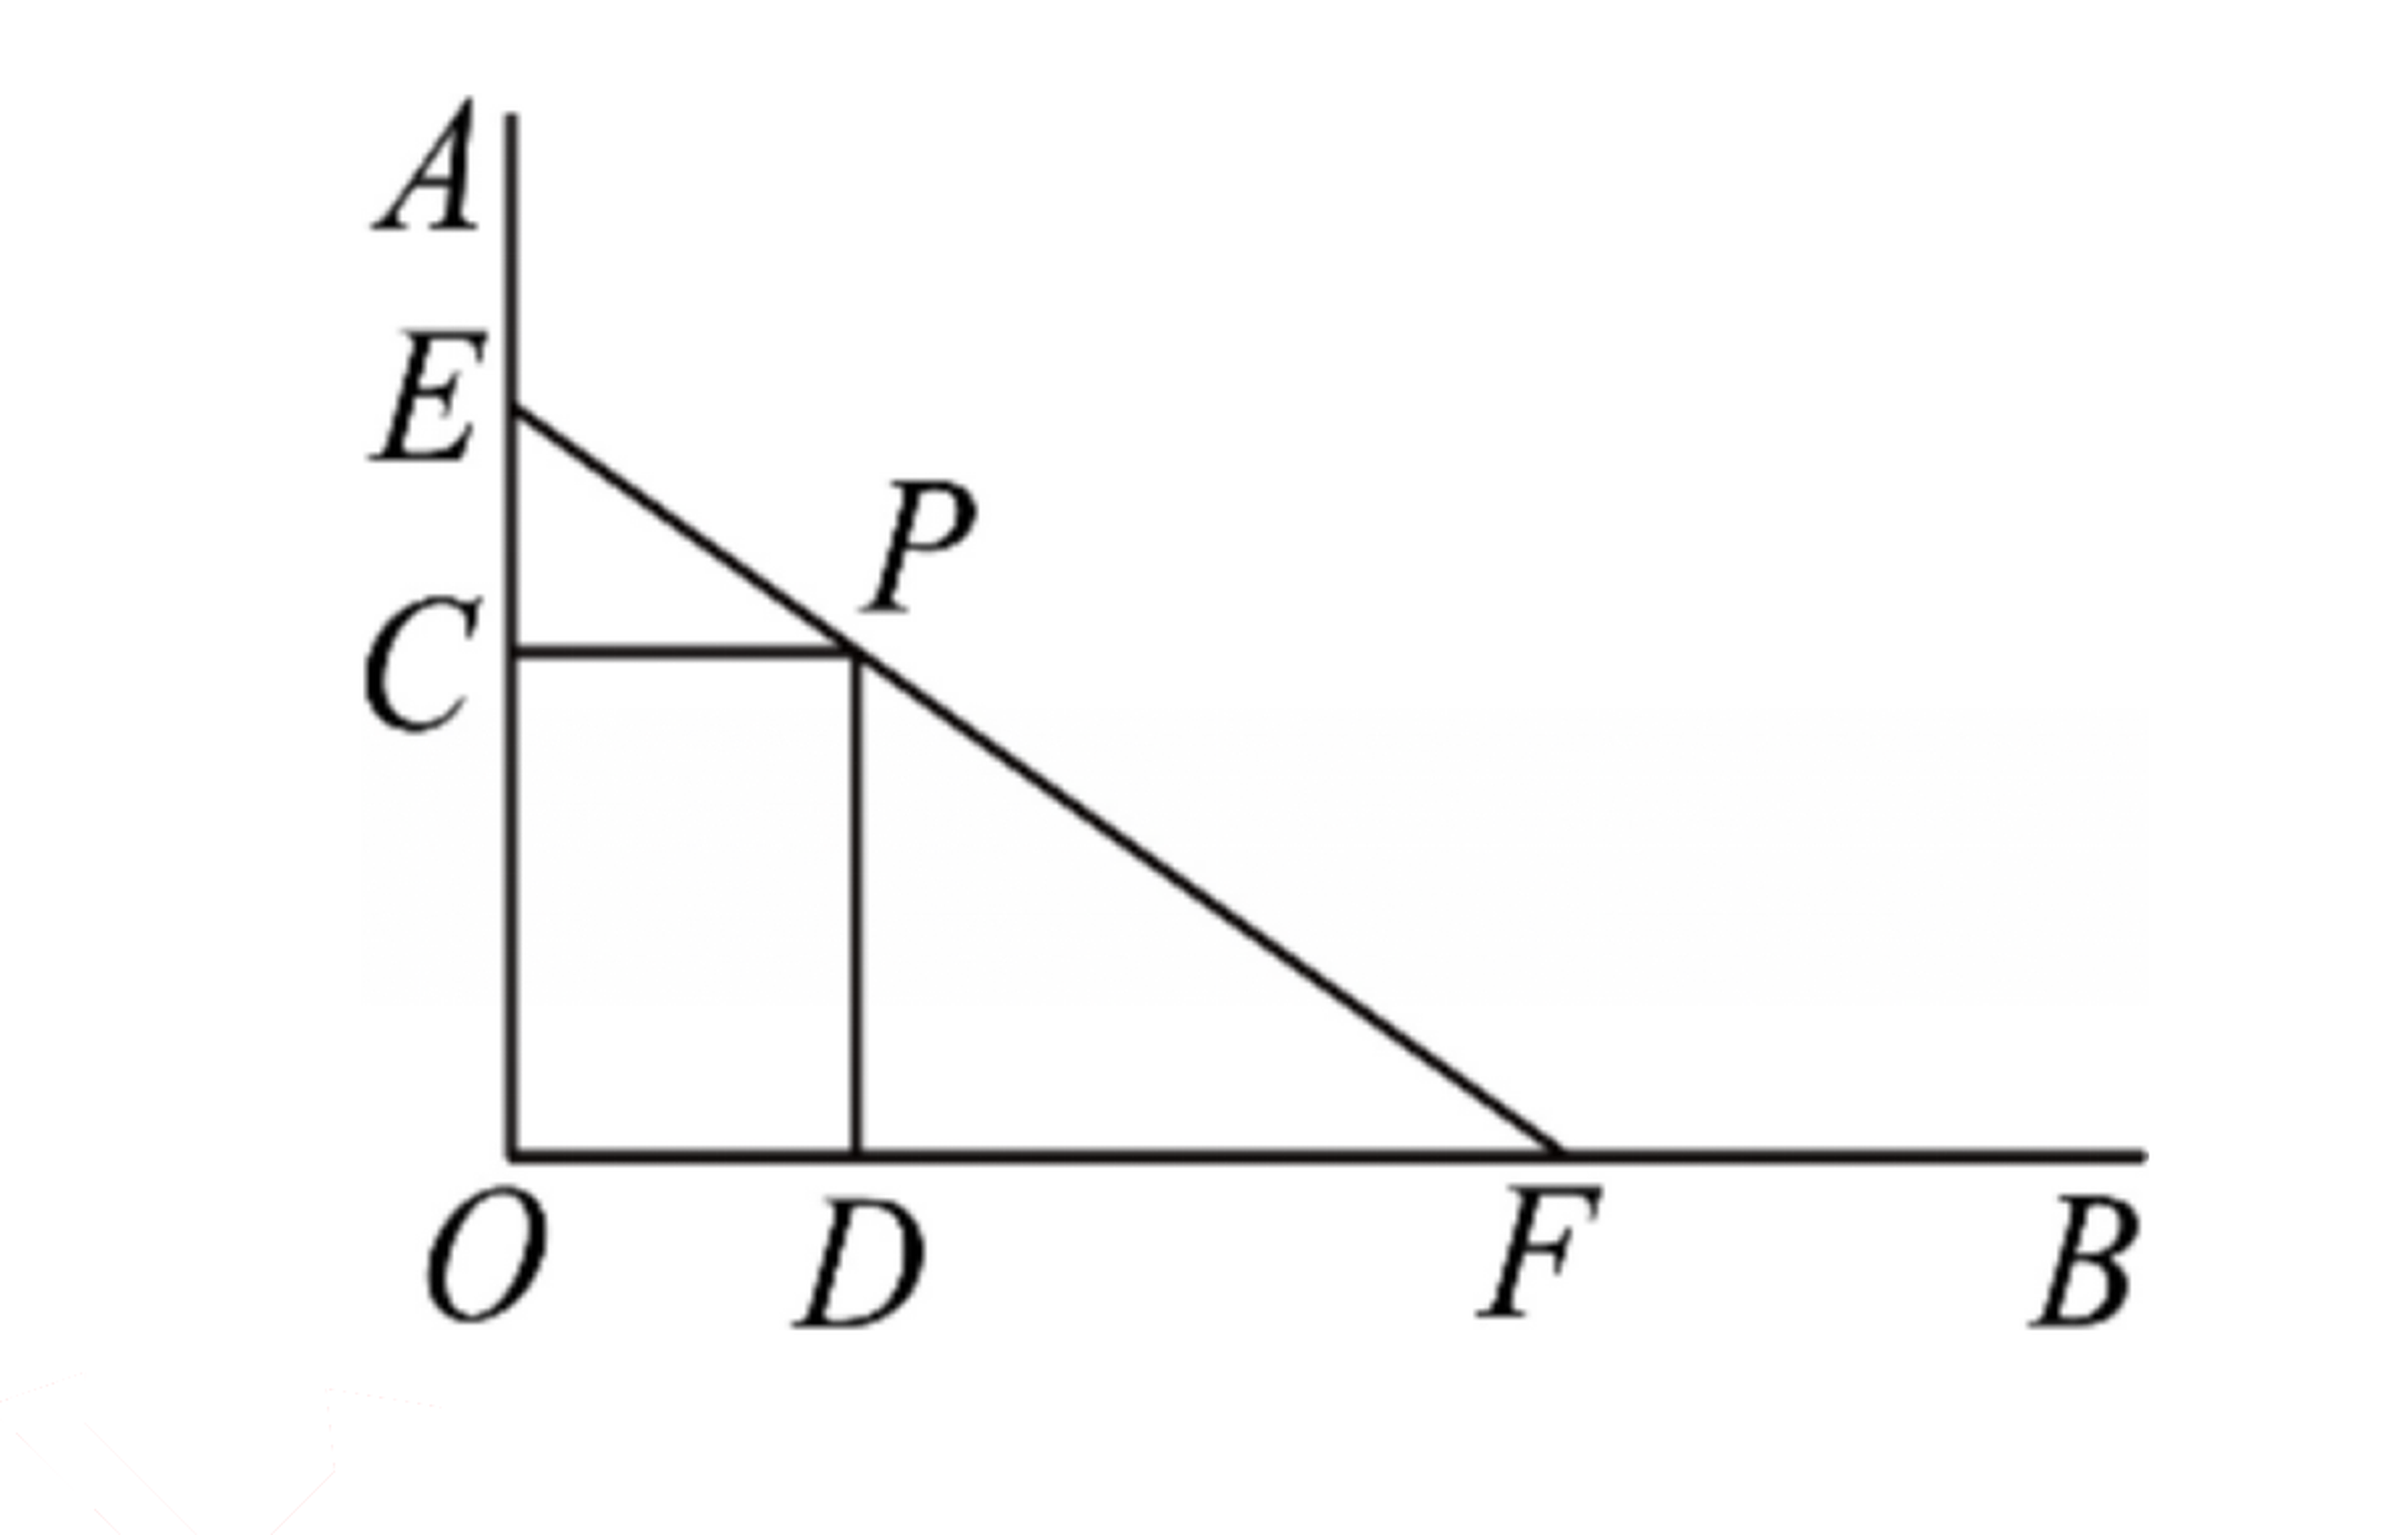
\includegraphics[width=0.32\textwidth]{figures/gao131_q19.png}
\end{center}

\ifanswer
\solbegin
\step{(1) 由题意得 $x\leq60$，}
\step{$\triangle PCE\sim\triangle FDP$，所以 $\dfrac{EC}{CP}=\dfrac{PD}{DF}$，即 $\dfrac{x}{25}=\dfrac{40}{DF}$，得 $DF=\dfrac{1000}{x}$m，}
\step{所以 $OF=OD+DF=\left(25+\dfrac{1000}{x}\right)$m，}
\step{所以 $25+\dfrac{1000}{x}\leq100$，解得 $x\geq\dfrac{40}{3}$；}
\step{综上，$\dfrac{40}{3}\leq x\leq60$；}
\step{(2) 由 $OE=OC+CE=(40+x)$m，}
\step{所以 $S=\dfrac12 OF\cdot OE=\dfrac12\left(25+\dfrac{1000}{x}\right)(40+x)$}
\step{$=\dfrac12\left(1000+25x+\dfrac{40000}{x}+1000\right)$m$^2$，}
\step{由基本不等式得 $S\geq\dfrac12\left(2000+2\sqrt{25x\cdot\dfrac{40000}{x}}\right)=2000$m$^2$，}
\step{当且仅当 $25x=\dfrac{40000}{x}$，即 $x=40$ 时取等号，}
\step{故 $EC=40$m 时，$S$ 取得最小值，为 $2000$m$^2$.}
\solend
\fi

\item 已知 $a\in\R$，函数 $y=ax^2+(3a+2)x+2a+3$.

(1) 当 $a=1$ 时，函数 $y=ax^2+(3a+2)x+2a+3$ 的图象与 $x$ 轴交于 $A(x_1,0)$，$B(x_2,0)$ 两点，求 $x_1^3+x_2^3$；

(2) 若关于 $x$ 的不等式 $ax^2+(3a+2)x+2a+3>2x$ 的解集为 $\R$，求实数 $a$ 的取值范围；

(3) 求关于 $x$ 的不等式 $y\geq1$ 的解集.

\ifanswer
\solbegin
\step{(1) 函数 $y=ax^2+(3a+2)x+2a+3$，当 $a=1$ 时，$y=x^2+5x+5$，}
\step{因为 $y=x^2+5x+5$ 的图象与 $x$ 轴交于 $A(x_1,0)$，$B(x_2,0)$ 两点，}
\step{即 $x^2+5x+5=0$ 的两个根为 $x_1$、$x_2$，}
\step{由根与系数的关系得 $x_1+x_2=-5$，$x_1x_2=5$，}
\step{所以 $x_1^2+x_2^2=(x_1+x_2)^2-2x_1x_2=25-10=15$，}
\step{所以 $x_1^3+x_2^3=(x_1+x_2)(x_1^2+x_2^2-x_1x_2)=-5\times(15-5)=-50$；}
\step{(2) 不等式 $ax^2+(3a+2)x+2a+3>2x$ 恒成立，得 $ax^2+3ax+2a+3>0$.}
\step{当 $a=0$ 时，$3>0$，恒成立，符合题意；}
\step{当 $a\neq0$ 时，若 $a<0$，二次函数 $ax^2+3ax+2a+3$ 开口向下，}
\step{一定存在小于零的部分，故不满足题意；}
\step{当 $a>0$ 时，若使 $ax^2+3ax+2a+3>0$ 恒成立，}
\step{只需 $\Delta=(3a)^2-4\times a\times(2a+3)=a^2-12a<0$，解得 $0<a<12$，}
\step{综上所述，$a$ 的取值范围为 $0\leq a<12$.}
\step{(3) 由 $y\geq1$，得 $ax^2+(3a+2)x+2a+3\geq1$，}
\step{即 $ax^2+(3a+2)x+2a+2\geq0$，即 $(ax+2a+2)(x+1)\geq0$，}
\step{当 $a=0$ 时，$2x+2\geq0$，解得 $x\geq-1$，}
\step{当 $a\neq0$ 时，}
\step{方程 $ax^2+(3a+2)x+2a+2=0$ 即为 $(x+1)(ax+2a+2)=0$，}
\step{解得 $x=-1$ 或 $x=-2-\dfrac2a$，令 $-1=-2-\dfrac2a$，即 $a=-2$，}
\step{当 $a>0$ 时，$-2-\dfrac2a<-1$，}
\step{不等式 $ax^2+(3a+2)x+2a+2\geq0$ 即为 $\left(x+\dfrac{2a+2}a\right)(x+1)\geq0$，}
\step{解得 $x\leq-2-\dfrac2a$ 或 $x\geq-1$；}
\step{当 $a<0$ 时，当 $-2-\dfrac2a<-1$，即 $a<-2$ 时，}
\step{不等式 $ax^2+(3a+2)x+2a+2\geq0$，即为 $\left(x+\dfrac{2a+2}a\right)(x+1)\leq0$，}
\step{解得 $-2-\dfrac2a\leq x\leq-1$；}
\step{当 $-2-\dfrac2a=-1$，即 $a=-2$，}
\step{不等式 $ax^2+(3a+2)x+2a+2\geq0$ 即为 $-2x^2-4x-2\geq0$，解得 $x=-1$，}
\step{当 $-2-\dfrac2a>-1$，即 $-2<a<0$ 时，}
\step{不等式 $ax^2+(3a+2)x+2a+2\geq0$ 即为 $\left(x+\dfrac{2a+2}a\right)(x+1)\leq0$，}
\step{解得 $-1\leq x\leq-2-\dfrac2a$，}
\step{综上所述，当 $a=0$ 时，解集为 $\{x\mid x\geq-1\}$；}
\step{当 $a>0$ 时，解集为 $\{x\mid x\leq-2-\dfrac2a$ 或 $x\geq-1\}$；}
\step{当 $a<-2$ 时，解集为 $\{x\mid -2-\dfrac2a\leq x\leq-1\}$；}
\step{当 $a=-2$ 时，解集为 $\{x\mid x=-1\}$；}
\step{当 $-2<a<0$ 时，解集为 $\{x\mid -1\leq x\leq-2-\dfrac2a\}$.}
\solend
\fi

\item 仔细阅读以下材料：【已知 $a$、$b\in(0,+\infty)$，$a+b=1$，求 $y=\dfrac1a+\dfrac2b$ 的最小值.

$y=\dfrac1a+\dfrac2b=\left(\dfrac1a+\dfrac2b\right)(a+b)=\dfrac ba+\dfrac{2a}b+3\geq3+2\sqrt2$，当且仅当 $\dfrac ba=\dfrac{2a}b$，即 $a=\sqrt2-1$，$b=2-\sqrt2$ 时取得等号，则 $y=\dfrac1a+\dfrac2b$ 的最小值为 $3+2\sqrt2$.

另 $y=\dfrac1a+\dfrac2b=\dfrac{a+b}a+\dfrac{2(a+b)}b=\dfrac ba+\dfrac{2a}b+3\geq3+2\sqrt2$，当且仅当 $\dfrac ba=\dfrac{2a}b$，即 $a=\sqrt2-1$，$b=2-\sqrt2$ 时取得等号，则 $y=\dfrac1a+\dfrac2b$ 的最小值为 $3+2\sqrt2$.】参考上述解法，求解下列问题.

(1) 若正实数 $x$、$y$ 满足 $x+y=1$，求 $\dfrac2x+\dfrac3y$ 的最小值；

(2) 已知 $x\in\left(0,\dfrac12\right)$，求 $t=\dfrac1x+\dfrac8{1-2x}$ 的最小值，并写出此时 $x$ 的值；

(3) 已知 $a$、$b\in(0,+\infty)$，$a+2b=1$，求 $p=\dfrac1{3a+4b}+\dfrac1{a+3b}$ 的最小值.

\ifanswer
\solbegin
\step{(1) 因为 $x>0,y>0$，且 $x+y=1$，}
\step{所以 $\dfrac2x+\dfrac3y=\left(\dfrac2x+\dfrac3y\right)(x+y)=2+\dfrac{2y}x+\dfrac{3x}y+3=5+\dfrac{2y}x+\dfrac{3x}y$，}
\step{由基本不等式得 $\dfrac{2y}x+\dfrac{3x}y\geq2\sqrt{\dfrac{2y}x\cdot\dfrac{3x}y}=2\sqrt6$，}
\step{当且仅当 $\dfrac{2y}x=\dfrac{3x}y$，即 $2y^2=3x^2$ 时，等号成立，}
\step{又因为 $x>0,y>0$ 且 $x+y=1$，此时 $x=\sqrt6-2,y=3-\sqrt6$，}
\step{所以 $\dfrac2x+\dfrac3y\geq5+2\sqrt6$，故 $\dfrac2x+\dfrac3y$ 的最小值为 $5+2\sqrt6$.}
\step{(2) 由 $0<x<\dfrac12$，则 $t=\dfrac1x+\dfrac8{1-2x}=\dfrac{2(1-2x+2x)}{2x}+\dfrac{8(1-2x+2x)}{1-2x}$}
\step{$=10+\dfrac{2\cdot(1-2x)}{2x}+\dfrac{8\cdot2x}{1-2x}\geq10+2\sqrt{\dfrac{2\cdot(1-2x)}{2x}\cdot\dfrac{8\cdot2x}{1-2x}}=18$，}
\step{当且仅当 $\dfrac{2\cdot(1-2x)}{2x}=\dfrac{8\cdot2x}{1-2x}$，即 $x=\dfrac16$ 时等号成立；}
\step{(3) 由 $a$、$b>0$，$a+2b=1$，则 $a=1-2b>0$，即 $0<b<\dfrac12$，}
\step{所以 $p=\dfrac1{3a+4b}+\dfrac1{a+3b}=\dfrac1{3a+6b-2b}+\dfrac1{a+2b+b}=\dfrac1{3-2b}+\dfrac1{1+b}$}
\step{$=\dfrac1{3-2b}+\dfrac2{2+2b}$，显然 $3-2b$、$2+2b>0$，}
\step{所以 $p=\dfrac15\cdot(3-2b+2+2b)\cdot\left(\dfrac1{3-2b}+\dfrac2{2+2b}\right)=\dfrac15\left[3+\dfrac{2+2b}{3-2b}+\dfrac{2(3-2b)}{2+2b}\right]$}
\step{$\geq\dfrac15\left[3+2\sqrt{\dfrac{2+2b}{3-2b}\cdot\dfrac{2(3-2b)}{2+2b}}\right]=\dfrac{3+2\sqrt2}5$，}
\step{当且仅当 $\dfrac{2+2b}{3-2b}=\dfrac{2(3-2b)}{2+2b}$，}
\step{即 $b=\dfrac{8-5\sqrt2}2$，$a=5\sqrt2-7$ 时等号成立.}
\solend
\fi

\end{enumerate}

\end{document}
"
%
% 原始材料：微信公众号"魔都数学加油站"文章，作者破晓，2026-11-13 18:18 发布；
% 连载"27学年高一131"，原文标题"27学年高一131——2026-2027年上海市六十中学高一上期中"；
% 原文链接：https://mp.weixin.qq.com/s/Nrbp3Uvt-sOGnOp4MEHemA。
% 正文为 11 张 PNG 页（01—05、09—11 为 2560x3620，06—08 为 4762x6735），
% 题目下印有【解析】或【答案】，为讲评版。题目、解析均据原图转录；
% 卷面粉红色水印"魔都数学加油站"及公众号页脚未录入。全卷仅第 19 题有 1 幅插图
% （矩形 OCPD 与小路 EF 的示意图），取 07.png 截图去水印。
%
% 卷首标题：原卷印作"2026-2027 年六十中学高一上期中"（公众号标题中的"上海市"
% 卷面标题行没有，本稿照卷面），年份区间按全稿惯例排 en dash；原卷未印副标题，
% 本卷为期中卷、跨集合与常用逻辑用语／不等式／函数三章，按题目内容标为
% "集合与常用逻辑用语、不等式、函数"（与 125／126／128／129 同期中卷口径相同）：
% 集合与逻辑见 Q3、Q4、Q7、Q13、Q17，不等式见 Q8、Q10、Q12、Q14、Q15、Q16、Q19、
% Q20、Q21，函数（指数／对数／幂函数、基本不等式应用）见 Q5、Q6、Q9、Q11、Q18、Q21。
%
% 题号体例：本卷共 19 题——一、填空题 3—12（10 题）、二、选择题 13—16（4 题）、
% 三、解答题 17—21（5 题）。三节分别 \setcounter{enumi}{2}／{12}／{16}。
%
% 与原卷的排版差异：
%   ① 原文从第 3 题起，本稿保留原题号（见上"题号体例"）；
%   ② 原卷每题下直接印【解析】／【答案】，本稿按全稿惯例置于答案版；第 3、4 题只印
%      【答案】，另提 \ans{}；第 13—16 题答案在解析末句"故选 …"，题干括号内留空、
%      不另提 \ans{}；其余各题印【解析】、无独立答案段；
%   ③ 原卷未印副标题，本稿按"知识模块"口径补出；
%   ④ 原卷填空横线按全稿惯例排为 \blankline[4.4em]；选择题括号排 \mbox{（\quad）}、
%      选项段前按惯例加 \keepwithprev；解答题不留作答区（原卷为讲评版，与 109—129 同）；
%   ⑤ 原卷数集排斜体 $R$／$N$，按全稿惯例改 \R／\N；绝对值排 \lvert…\rvert，
%      集合描述竖线排 \mid；不等号按全稿惯例排 \leqslant／\geqslant；
%   ⑥ 子题标号 (1)(2)(3) 原卷用半角括号，照录；圈数字 ①② 照录；
%   ⑦ 原卷第 19 题插图浮排在第 07 页题干右侧，本稿按体例就近置于题干"如图"之后
%      （居中 \includegraphics），图取原卷 07 页截图去水印；题前按惯例加
%      \needvspace{7cm} 守卫（照 高一120／127／129 成例），保证"题干 + 图"整块不被页边界切开；
%   ⑧ 原卷 Q9 题干跨 01—02 页、Q15 解析跨 03—04 页、Q16 材料跨 04—05 页、
%      Q17 题干跨 05—06 页、Q20 解析跨 08—09 页、Q21 解析跨 09—11 页，
%      本稿按题合并连续排版；末页第 11 页为 Q21 (3) 解析的续尾，按实际印刷行单列。
%   ⑨ 第 16 题材料英文括注原卷印作 (Cauchy – SchwarzInequality)（长横、Schwarz 与
%      Inequality 斜体连排无空格），本稿按全稿英文专名惯例排 \emph{(Cauchy-Schwarz Inequality)}；
%      第 15 题解析 B、D 两行原卷各印一步含 \lg m 的换底繁分数（2026-11-13 回原图核对补回，
%      本稿初转曾顺手去重跳过该步）。
%
% 判别式字形：第 20 题 (2) 解析 $\Delta=(3a)^2-4\times a\times(2a+3)=a^2-12a<0$
%   原卷排三角形（等腰、高；回 08.png 放大核对），照录 \Delta；全卷判别式仅此一处
%   （\triangle 另作第 19 题「$\triangle PCE\sim\triangle FDP$」的几何三角形记号）。
%
% 子集符号：第 17 题 (2) 解析 $P\subseteq Q$ 印带下划线，照录 \subseteq；
%   全卷未出现单线 \subset。
%
% 原卷存疑照录：
%   第 11 题解析末两式作 $\dfrac{2+m+\frac1n}{2n+2}=\dfrac{2n+mn+1}{2n+2}$，而第三式
%     分母 $\log_3 9+\log_3 2+\log_3 2=2+\frac2n$，与前一分母 $2n+2$ 不等，照录；
%   第 16 题材料 ①"对于所有实数 $x$ 和 $y$，有 $(a^2+b^2)(c^2+d^2)\geq(ac+bd)^2$"
%     句首用 $x$、$y$ 而式中用 $a$、$b$、$c$、$d$，照录；
%   第 20 题题干 (2) 作"解集为 $\R$"、解析 (2) 作"恒成立"，措辞不同，照录；
%   第 21 题材料把同一道题用两种解法连印两遍（"另 $y=\frac1a+\frac2b=\dots$"），照录；
%   第 21 题 (3) 解析末句"即 $b=\frac{8-5\sqrt2}{2}$，$a=5\sqrt2-7$ 时等号成立"
%     未另写"故最小值为 $\frac{3+2\sqrt2}{5}$"，照录；
%   第 12 题解析"所以 $e^a+e^b>e^c, a+b>c$"、第 8 题解析"$a>0$，$b>0$"、
%     第 18 题 (2)"$4x^2-4x+1<x^2+4x+4$，解得 $-\frac13<x<3$"等处数学式内
%     半角逗号，照录；
%   第 15 题解析用 $\lg$ 记常用对数（$\lg m$、$\lg 3$、$\lg 5$、$\lg 15$），照录。
%
% 行数复核：逐题数 \step 条数，合计 119 条（Q3：0；Q4：0；Q5：1；Q6：1；Q7：2；
% Q8：2；Q9：1；Q10：1；Q11：2；Q12：6；Q13：2；Q14：3；Q15：14；Q16：10；
% Q17：4；Q18：8；Q19：11；Q20：35；Q21：16），与原卷印刷行逐题相等
% （cases 块作一个印刷行计）。第 3、4 题只印【答案】，提 \ans{}，不计入 \step 账；
% 四道选择题答案均在解析末句，括号内留空、不另提 \ans{}。
%
\documentclass[a4paper,11pt]{article}
\usepackage{common}

\begin{document}

\examtitlest[3]{2026--2027 年六十中学高一上期中}{集合与常用逻辑用语、不等式、函数}

\bigsec{一、填空题}

\begin{enumerate}
\setcounter{enumi}{2}

\item 已知集合 $A=(0,4),B=[2,5]$，则 $A\cup B=$\blankline[4.4em].

\ifanswer
\ans{$(0,5]$}
\fi

\item 陈述句“$x=2$ 或 $y=3$”的否定形式为\blankline[4.4em].

\ifanswer
\ans{$x\neq2$ 且 $y\neq3$}
\fi

\item 函数 $y=a^{x-2}+15(a>0$ 且 $a\neq1)$ 的图象恒过定点的坐标为\blankline[4.4em].

\ifanswer
\solbegin
\step{函数 $y=a^{x-2}+15$ 的图象恒过定点 $A(2,16)$.}
\solend
\fi

\item 用有理数指数幂的形式来化简：$\dfrac{\sqrt{a\cdot\sqrt[3]{a^4}}}{\left(a^{\frac13}\right)^2}=$\blankline[4.4em].

\ifanswer
\solbegin
\step{原式 $=\dfrac{\sqrt{a\cdot a^{\frac43}}}{a^{\frac23}}=\dfrac{\sqrt{a^{\frac73}}}{a^{\frac23}}=\dfrac{a^{\frac76}}{a^{\frac23}}=a^{\frac76-\frac23}=a^{\frac12}(a>0)$.}
\solend
\fi

\item 已知集合 $A=\left\{x\mid \dfrac6{6-x}\in\N\text{ 且 }x\in\N\right\}$，则用列举法表示集合 $A=$\blankline[4.4em].

\ifanswer
\solbegin
\step{当 $x=0$ 时，$\dfrac6{6-0}=1\in\N$，当 $x=3$ 时，$\dfrac6{6-3}=2\in\N$，}
\step{当 $x=4$ 时，$\dfrac6{6-4}=3\in\N$，当 $x=5$ 时，$\dfrac6{6-5}=6\in\N$，故 $A=\{0,3,4,5\}$.}
\solend
\fi

\item 已知 $a>0$，$b>0$，且 $ab=\dfrac12$，则 $\dfrac1a+\dfrac8b$ 的最小值是\blankline[4.4em].

\ifanswer
\solbegin
\step{$a>0$，$b>0$，且 $ab=\dfrac12$，则 $\dfrac1a+\dfrac8b\geq2\sqrt{\dfrac8{ab}}=8$，}
\step{当且仅当 $\dfrac1a=\dfrac8b$，即 $a=\dfrac14,b=2$ 时取等号，故最小值为 $8$.}
\solend
\fi

\item 心理学家有时用函数 $L(t)=A(1-e^{-kt})$ 测定在时间 $t$（单位：$min$）内能够记忆的量 $L$，其中 $A$ 表示需要记忆的量，$k$ 表示记忆率. 假设一个学生需要记忆的量为 $200$ 个单词，此时 $L$ 表示在时间 $t$ 内该生能够记忆的单词个数. 已知该生在 $5min$ 内能够记忆 $20$ 个单词，则 $k$ 的值约为\blankline[4.4em]（结果保留四位小数）.

\ifanswer
\solbegin
\step{由题意得 $200(1-e^{-5k})=20$，所以 $e^{-5k}=0.9$，解得 $k\approx0.0211$.}
\solend
\fi

\item 设 $x\in\R$，方程 $\lvert 3x-2\rvert+\lvert 1-x\rvert=\lvert 2x-1\rvert$ 的解集是\blankline[4.4em].

\ifanswer
\solbegin
\step{由三角不等式得 $(3x-2)(1-x)\geq0$，故解集是 $\left[\dfrac23,1\right]$.}
\solend
\fi

\item 已知 $3^m=5$，$n=\log_2 3$，则 $\log_{36}90$ 可用 $m$、$n$ 表示为\blankline[4.4em].

\ifanswer
\solbegin
\step{由 $3^m=5$，又 $n=\log_2 3$，得 $m=\log_3 5$，$\log_3 2=\dfrac{\log_2 2}{\log_2 3}=\dfrac1n$，}
\step{所以 $\log_{36}90=\dfrac{\log_3 90}{\log_3 36}=\dfrac{\log_3 9+\log_3 2+\log_3 5}{\log_3 9+\log_3 2+\log_3 2}=\dfrac{2+m+\frac1n}{2n+2}=\dfrac{2n+mn+1}{2n+2}$.}
\solend
\fi

\item 若定义域为 $I=(0,m]$ 的函数 $f(x)=e^x$ 满足：对任意能构成三角形三边长的实数 $a$、$b$、$c\in I$，均有 $f(a)$、$f(b)$、$f(c)$ 也能构成三角形三边长，则 $m$ 的最大值为\blankline[4.4em].

\ifanswer
\solbegin
\step{$f(x)=e^x$ 在 $I=(0,m]$ 上严格增，所以 $f(x)\in(1,e^m]$，不妨设 $0<a\leq b\leq c$，}
\step{因为对任意能构成三角形三边长的实数 $a,b,c\in I$，均有 $f(a)$，$f(b)$，$f(c)$}
\step{也能构成三角形三边长，所以 $e^a+e^b>e^c, a+b>c$，}
\step{因为 $e^a+e^b\geq2\sqrt{e^ae^b}=2\sqrt{e^{a+b}}>e^c$，所以 $4e^{a+b}>e^{2c}$，}
\step{因为对任意 $a,b,c\in I$ 都成立，所以 $4e^c\geq e^{2c}$，所以 $e^c\leq4$，所以 $c\leq\ln4$，}
\step{所以 $m\leq\ln4$，所以 $m$ 的最大值为 $\ln4$.}
\solend
\fi

\end{enumerate}

\bigsec{二、选择题}

\begin{enumerate}
\setcounter{enumi}{12}

\item 已知 $m,n$ 是非零自然数，命题 $\alpha:mn$ 是奇数，命题 $\beta:m$ 或 $n$ 是奇数，则 $\alpha$ 是 $\beta$ 的\mbox{（\quad）}

\keepwithprev
A. 充分非必要条件\qquad\qquad B. 必要非充分条件

C. 充要条件\qquad\qquad D. 既非充分又非必要条件

\ifanswer
\solbegin
\step{$mn$ 是奇数 $\Leftrightarrow$ $m$、$n$ 都是奇数，所以 $\alpha$ 能推出 $\beta$，充分性成立，}
\step{但 $\beta$ 推不出 $\alpha$，必要性不成立，所以 $\alpha$ 是 $\beta$ 的充分非必要条件. 故选 $A$.}
\solend
\fi

\item 关于 $x$ 的不等式 $x^2-mx+n+5\leq0$ 的解集是 $[1,8]$，那么 $\log_m n=$\mbox{（\quad）}

\keepwithprev
A. $\dfrac13$\qquad\qquad B. $-3$\qquad\qquad C. $-2$\qquad\qquad D. $\dfrac12$

\ifanswer
\solbegin
\step{由题意得 $x^2-mx+n+5=0$ 的解为 $1$，$8$，}
\step{由根与系数的关系得 $\begin{cases}1+8=m\\1\times8=n+5\end{cases}$，解得 $m=9$，$n=3$，}
\step{所以 $\log_m n=\log_9 3=\dfrac12\log_3 3=\dfrac12$. 故选 $D$.}
\solend
\fi

\item 已知正实数 $x$、$y$、$z$ 满足 $3^x=5^y=15^z$，则下列说法中不正确的是\mbox{（\quad）}

\keepwithprev
A. $\dfrac1x+\dfrac1y=\dfrac1z$\qquad\qquad B. $x+y>2z$\qquad\qquad C. $3x>5y>15z$\qquad\qquad D. $x\cdot y>4z^2$

\ifanswer
\solbegin
\step{已知正实数 $x$、$y$、$z$，则设 $3^x=5^y=15^z=m>1$，}
\step{所以 $x=\log_3 m$，$y=\log_5 m$，$z=\log_{15} m$，}
\step{对于 $A$，$\dfrac1x+\dfrac1y=\dfrac1{\log_3 m}+\dfrac1{\log_5 m}=\log_m 3+\log_m 5=\log_m 15=\dfrac1z$，故 $A$ 正确；}
\step{对于 $B$，因为 $\dfrac{x+y}{z}=\dfrac{x}{z}+\dfrac{y}{z}=\dfrac{\log_3 m}{\log_{15} m}+\dfrac{\log_5 m}{\log_{15} m}=\dfrac{\dfrac{\lg m}{\lg3}}{\dfrac{\lg m}{\lg15}}+\dfrac{\dfrac{\lg m}{\lg5}}{\dfrac{\lg m}{\lg15}}=\dfrac{\lg15}{\lg3}+\dfrac{\lg15}{\lg5}$，}
\step{$=\dfrac{\lg3+\lg5}{\lg3}+\dfrac{\lg3+\lg5}{\lg5}=2+\dfrac{\lg5}{\lg3}+\dfrac{\lg3}{\lg5}=2+\log_3 5+\log_5 3$，}
\step{又 $\log_3 5>0$，$\log_5 3>0$，所以 $2+\log_3 5+\log_5 3>2$，}
\step{所以 $\dfrac{x+y}{z}>2$，即 $x+y>2z$，故 $B$ 正确；}
\step{对于 $C$，因为 $\dfrac5x=5\log_m 3=\log_m 243$，$\dfrac3y=3\log_m 5=\log_m 125$，}
\step{所以 $\dfrac5x>\dfrac3y$，即 $3x<5y$，故 $C$ 错误；}
\step{对于 $D$，$\dfrac{xy}{z^2}=\dfrac{x}{z}\cdot\dfrac{y}{z}=\dfrac{\log_3 m}{\log_{15} m}\cdot\dfrac{\log_5 m}{\log_{15} m}=\dfrac{\dfrac{\lg m}{\lg3}}{\dfrac{\lg m}{\lg15}}\cdot\dfrac{\dfrac{\lg m}{\lg5}}{\dfrac{\lg m}{\lg15}}=\dfrac{\lg15}{\lg3}\cdot\dfrac{\lg15}{\lg5}$}
\step{$=\dfrac{\lg3+\lg5}{\lg3}\cdot\dfrac{\lg3+\lg5}{\lg5}=\left(1+\dfrac{\lg5}{\lg3}\right)\left(1+\dfrac{\lg3}{\lg5}\right)=2+\dfrac{\lg5}{\lg3}+\dfrac{\lg3}{\lg5}$}
\step{$\geq2+2\sqrt{\dfrac{\lg5}{\lg3}\cdot\dfrac{\lg3}{\lg5}}=2+2=4$，又 $\lg3\neq\lg5$，故等号不成立，}
\step{所以 $\dfrac{xy}{z^2}>4$，即 $xy>4z^2$，故 $D$ 正确.}
\step{故选 $C$.}
\solend
\fi

\item 柯西不等式 \emph{(Cauchy-Schwarz Inequality)} 是一种在数学和物理学中广泛使用的不等式，它是由法国数学家奥古斯丁$\cdot$路易$\cdot$柯西提出的，柯西不等式可以用于证明其他不等式，也可以用于解决一些数学问题. 以下是柯西不等式的原始形式：

①对于所有实数 $x$ 和 $y$，有 $(a^2+b^2)(c^2+d^2)\geq(ac+bd)^2$.

②等式条件：当且仅当 $ad-bc=0$ 时，等号成立.

例：已知 $x+2y=2$，由柯西不等式 $(x^2+y^2)(1^2+2^2)\geq(x+2y)^2$，可得 $(x^2+y^2)_{min}=\dfrac45$.

现给出以下两个命题：

①若 $a^2+b^2=1$，则 $2a+3b$ 的最大值为 $\sqrt{13}$；

②若 $1<a<3$，则 $\sqrt{a-1}+\sqrt{6-2a}$ 的最大值为 $\sqrt6$；

则运用柯西不等式，判断以下正确的选项有\mbox{（\quad）}

\keepwithprev
A. ①为真命题；②为真命题\qquad\qquad B. ①为真命题；②为假命题

C. ①为假命题；②为真命题\qquad\qquad D. ①为假命题；②为假命题

\ifanswer
\solbegin
\step{由柯西不等式得 $(a^2+b^2)(2^2+3^2)\geq(2a+3b)^2$.}
\step{因为 $a^2+b^2=1$，所以 $(2^2+3^2)\geq(2a+3b)^2$，即 $13\geq(2a+3b)^2$，}
\step{所以 $-\sqrt{13}\leq2a+3b\leq\sqrt{13}$，则 $(2a+3b)_{max}=\sqrt{13}$，}
\step{当且仅当 $3a=2b$ 时取等号，故①正确.}
\step{令 $x=\sqrt{a-1}$，$y=\sqrt{3-a}$，则 $x^2+y^2=a-1+3-a=2$，}
\step{由柯西不等式得 $(\sqrt{a-1}+\sqrt{6-2a})^2=(\sqrt{a-1}+\sqrt2\cdot\sqrt{3-a})^2=(x+\sqrt2 y)^2$}
\step{$\leq[1^2+(\sqrt2)^2](x^2+y^2)$，}
\step{因为 $x^2+y^2=2$，所以 $(\sqrt{a-1}+\sqrt{6-2a})^2\leq6$，}
\step{当且仅当 $\sqrt{3-a}=\sqrt2\sqrt{a-1}$ 取等号，所以 $\sqrt{a-1}+\sqrt{6-2a}\leq\sqrt6$，故②正确.}
\step{故选 $A$.}
\solend
\fi

\end{enumerate}

\bigsec{三、解答题}

\begin{enumerate}
\setcounter{enumi}{16}

\item 已知集合 $P=\left\{x\mid \dfrac{3x-1}{x+2}<1\right\}$，集合 $Q=\{x\mid\lvert x-a\rvert\leq2\}$.

(1) 求集合 $P$；

(2) 若“$x\in P$”是“$x\in Q$”的充分非必要条件，求实数 $a$ 的取值范围.

\ifanswer
\solbegin
\step{(1) 集合 $P=\left\{x\mid \dfrac{3x-1}{x+2}<1\right\}$，得 $\dfrac{2x-3}{x+2}<0$，解得 $P=\left(-2,\dfrac32\right)$.}
\step{(2) 集合 $Q=\{x\mid\lvert x-a\rvert\leq2\}=\{x\mid a-2\leq x\leq2+a\}$，}
\step{由“$x\in P$”是“$x\in Q$”的充分非必要条件，得 $P\subseteq Q$，}
\step{得 $\begin{cases}-2\geq a-2\\\dfrac32\leq2+a\\a-2<2+a\end{cases}$，解得 $a\in\left[-\dfrac12,0\right]$.}
\solend
\fi

\item 已知幂函数 $f(x)=(m^2-4m+4)\cdot x^{2m-4}$ 在 $(-\infty,0)$ 上是严格减函数.

(1) 求函数 $y=f(x)$ 的解析式；

(2) 若 $f(1-2x)<f(x+2)$，求 $x$ 的取值范围.

\ifanswer
\solbegin
\step{(1) 由幂函数的定义得 $m^2-4m+4=1$，解得 $m=1$ 或 $3$，}
\step{当 $m=1$ 时，$f(x)=x^{-2}=\dfrac1{x^2}$，在 $(-\infty,0)$ 上严格增，不符合题意，}
\step{当 $m=3$ 时，$f(x)=x^2$，在 $(-\infty,0)$ 上严格减，符合题意，}
\step{所以 $f(x)=x^2$；}
\step{(2) 由函数 $f(x)=x^2$ 图象关于 $y$ 轴对称，且在 $[0,+\infty)$ 上严格增，}
\step{则 $f(1-2x)<f(x+2)$ 可化为 $\lvert1-2x\rvert<\lvert x+2\rvert$，}
\step{平方得 $4x^2-4x+1<x^2+4x+4$，解得 $-\dfrac13<x<3$，}
\step{所以 $x$ 的取值范围是 $\left(-\dfrac13,3\right)$.}
\solend
\fi

% 第 19 题是"题干 + 图"约 7cm 的一整块，守卫放在 \item 之前（放 \item 之后会失效）
\needvspace{7cm}
\item 如图，$OA$、$OB$ 是两条长度足够长的互相垂直的笔直小路，矩形 $OCPD$ 的顶点 $C$，$D$ 分别在 $OA$、$OB$ 上，且该矩形区域内种满了荷花. 为了让观赏者有更好的观赏体验，现计划经过点 $P$ 修一条小路 $EF$，其中点 $E$ 在小路 $OA$ 上，点 $F$ 在小路 $OB$ 上，并在 $\triangle OEF$ 区域内种满荷花. 已知 $OD=25m$，$OC=40m$，且小路 $EF$ 要完全位于一个以 $O$ 为顶点的，边长为 $100$ m 的正方形内部（包括边界）. 记 $\triangle OEF$ 的面积为 $S$m$^2$.

(1) 设 $EC=x\cdot m$，试用 $x$ 表示 $OF$，并求 $x$ 的取值范围.

(2) 当 $EC$ 的长度为多少时，$S$ 取得最小值？最小值是多少？

\begin{center}
% 图取原卷 07.png 截图去粉色水印，2.8× LANCZOS 放大
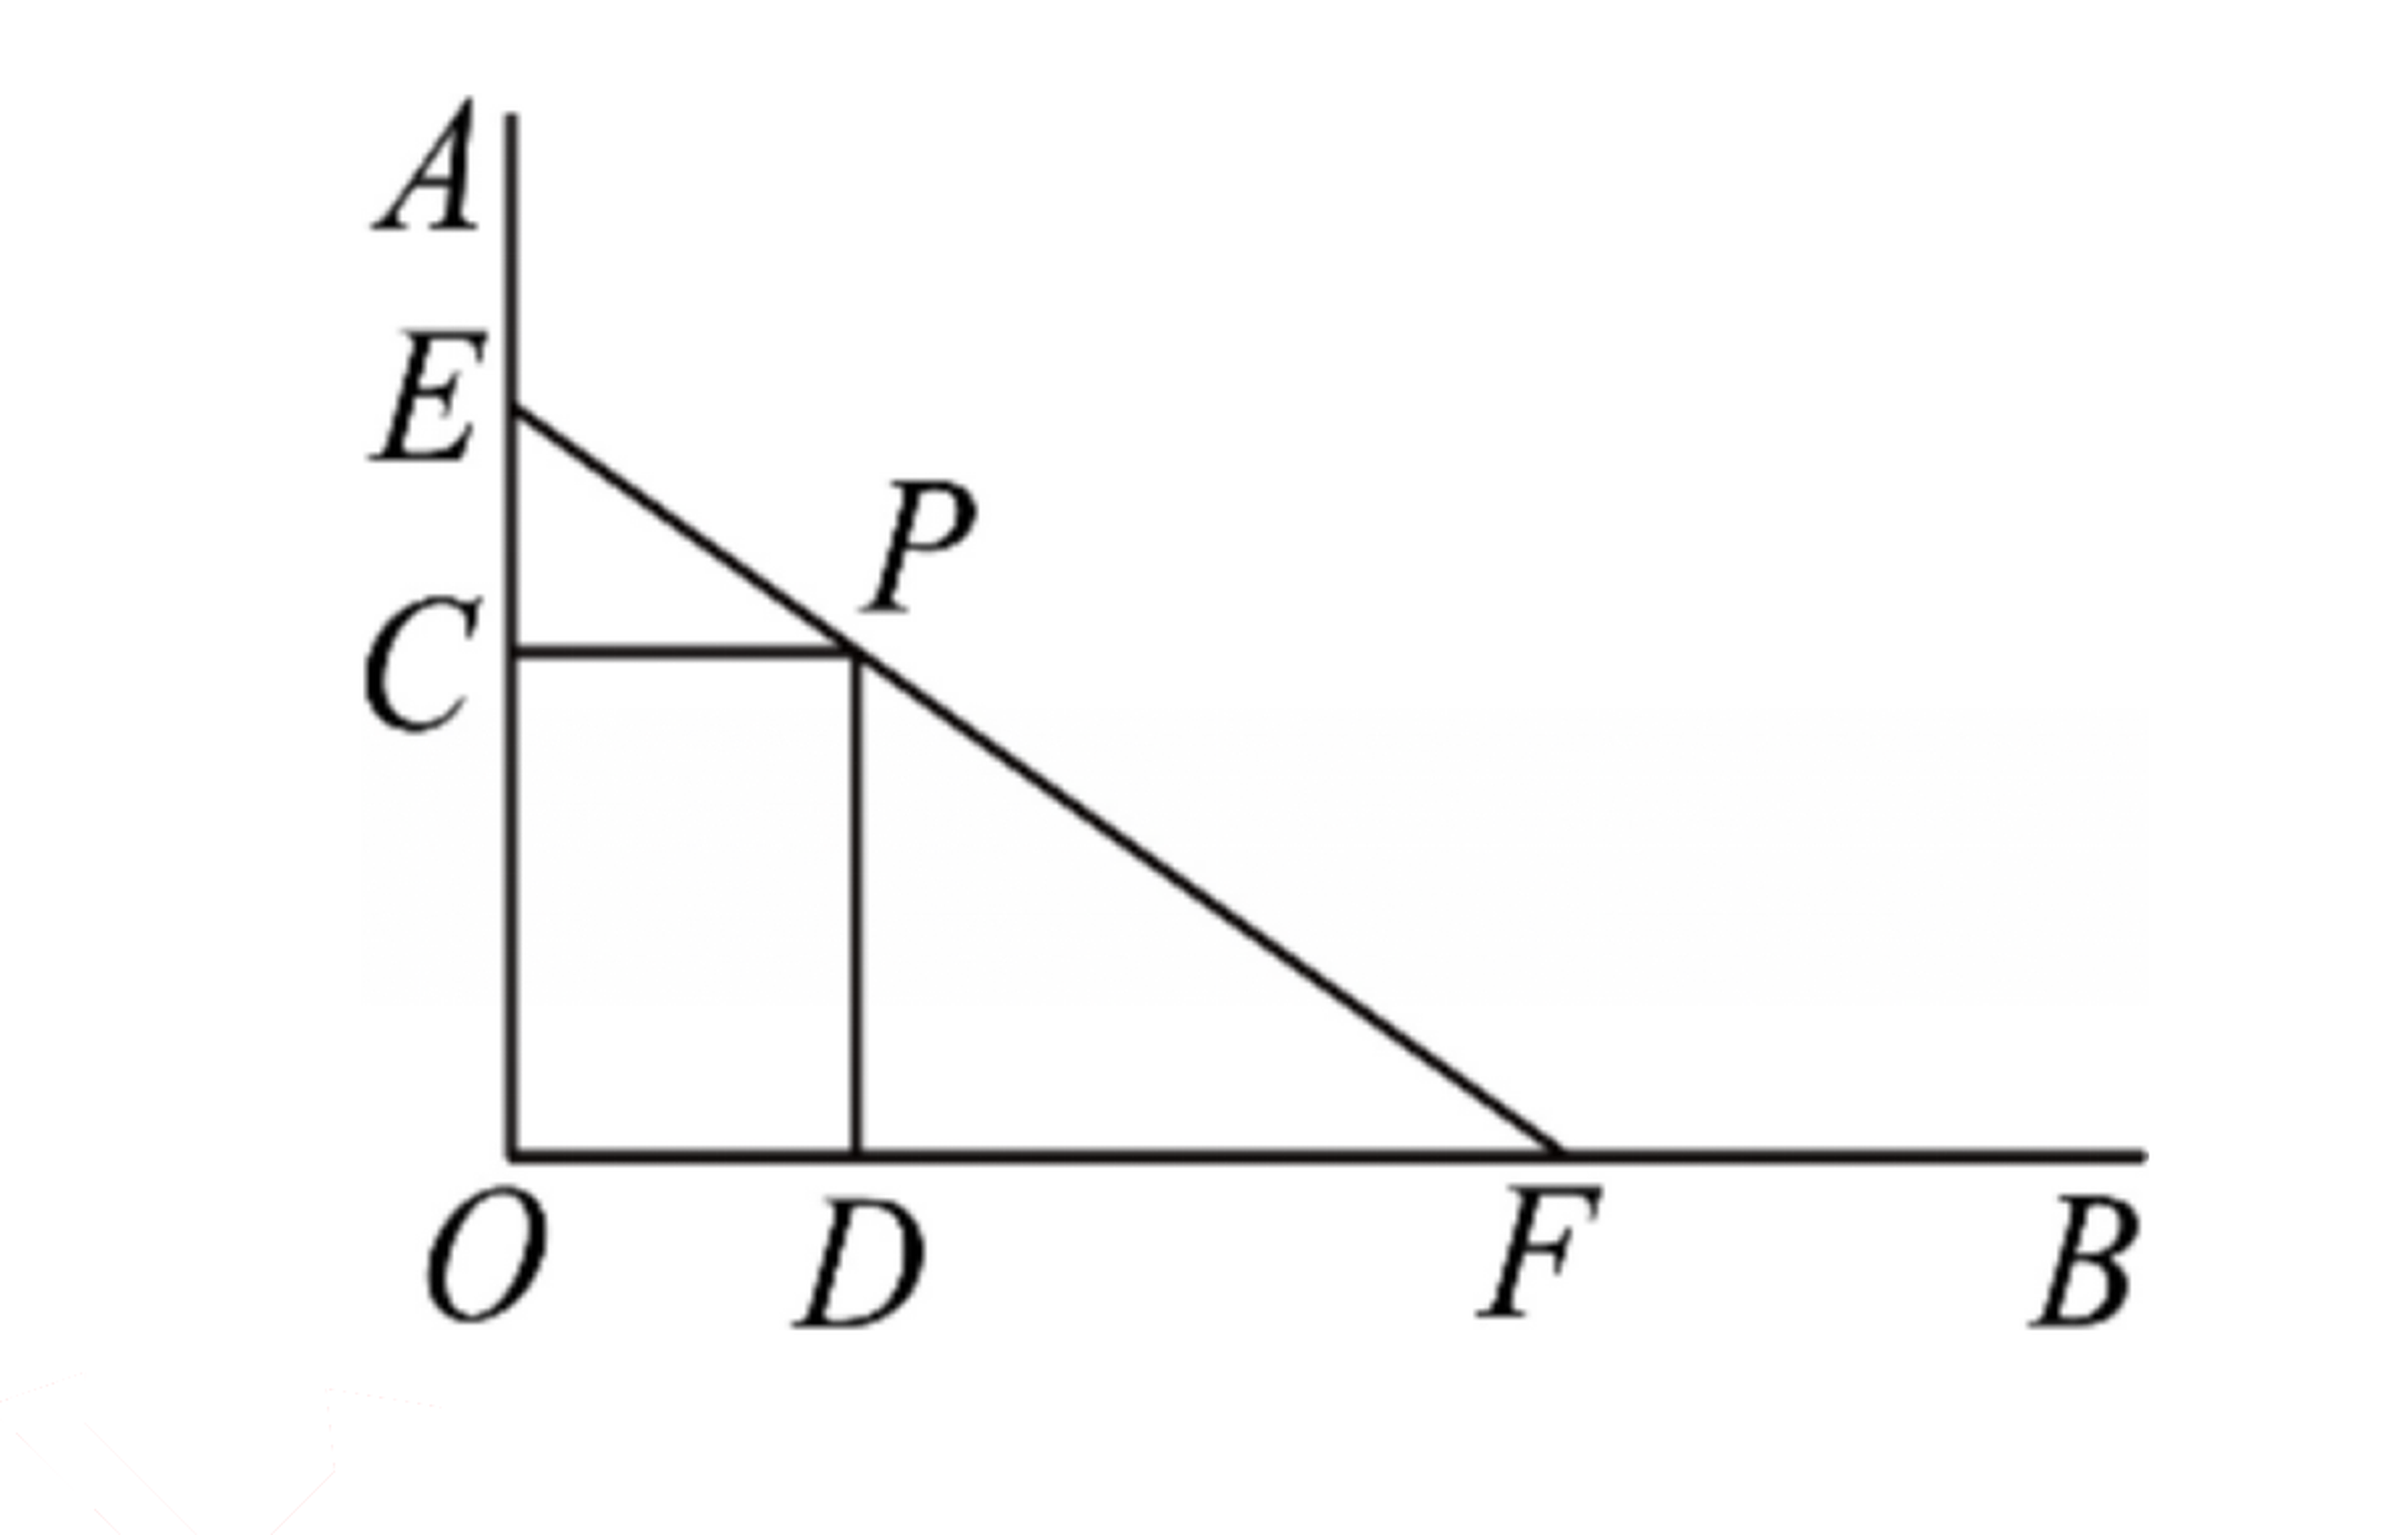
\includegraphics[width=0.32\textwidth]{figures/gao131_q19.png}
\end{center}

\ifanswer
\solbegin
\step{(1) 由题意得 $x\leq60$，}
\step{$\triangle PCE\sim\triangle FDP$，所以 $\dfrac{EC}{CP}=\dfrac{PD}{DF}$，即 $\dfrac{x}{25}=\dfrac{40}{DF}$，得 $DF=\dfrac{1000}{x}$m，}
\step{所以 $OF=OD+DF=\left(25+\dfrac{1000}{x}\right)$m，}
\step{所以 $25+\dfrac{1000}{x}\leq100$，解得 $x\geq\dfrac{40}{3}$；}
\step{综上，$\dfrac{40}{3}\leq x\leq60$；}
\step{(2) 由 $OE=OC+CE=(40+x)$m，}
\step{所以 $S=\dfrac12 OF\cdot OE=\dfrac12\left(25+\dfrac{1000}{x}\right)(40+x)$}
\step{$=\dfrac12\left(1000+25x+\dfrac{40000}{x}+1000\right)$m$^2$，}
\step{由基本不等式得 $S\geq\dfrac12\left(2000+2\sqrt{25x\cdot\dfrac{40000}{x}}\right)=2000$m$^2$，}
\step{当且仅当 $25x=\dfrac{40000}{x}$，即 $x=40$ 时取等号，}
\step{故 $EC=40$m 时，$S$ 取得最小值，为 $2000$m$^2$.}
\solend
\fi

\item 已知 $a\in\R$，函数 $y=ax^2+(3a+2)x+2a+3$.

(1) 当 $a=1$ 时，函数 $y=ax^2+(3a+2)x+2a+3$ 的图象与 $x$ 轴交于 $A(x_1,0)$，$B(x_2,0)$ 两点，求 $x_1^3+x_2^3$；

(2) 若关于 $x$ 的不等式 $ax^2+(3a+2)x+2a+3>2x$ 的解集为 $\R$，求实数 $a$ 的取值范围；

(3) 求关于 $x$ 的不等式 $y\geq1$ 的解集.

\ifanswer
\solbegin
\step{(1) 函数 $y=ax^2+(3a+2)x+2a+3$，当 $a=1$ 时，$y=x^2+5x+5$，}
\step{因为 $y=x^2+5x+5$ 的图象与 $x$ 轴交于 $A(x_1,0)$，$B(x_2,0)$ 两点，}
\step{即 $x^2+5x+5=0$ 的两个根为 $x_1$、$x_2$，}
\step{由根与系数的关系得 $x_1+x_2=-5$，$x_1x_2=5$，}
\step{所以 $x_1^2+x_2^2=(x_1+x_2)^2-2x_1x_2=25-10=15$，}
\step{所以 $x_1^3+x_2^3=(x_1+x_2)(x_1^2+x_2^2-x_1x_2)=-5\times(15-5)=-50$；}
\step{(2) 不等式 $ax^2+(3a+2)x+2a+3>2x$ 恒成立，得 $ax^2+3ax+2a+3>0$.}
\step{当 $a=0$ 时，$3>0$，恒成立，符合题意；}
\step{当 $a\neq0$ 时，若 $a<0$，二次函数 $ax^2+3ax+2a+3$ 开口向下，}
\step{一定存在小于零的部分，故不满足题意；}
\step{当 $a>0$ 时，若使 $ax^2+3ax+2a+3>0$ 恒成立，}
\step{只需 $\Delta=(3a)^2-4\times a\times(2a+3)=a^2-12a<0$，解得 $0<a<12$，}
\step{综上所述，$a$ 的取值范围为 $0\leq a<12$.}
\step{(3) 由 $y\geq1$，得 $ax^2+(3a+2)x+2a+3\geq1$，}
\step{即 $ax^2+(3a+2)x+2a+2\geq0$，即 $(ax+2a+2)(x+1)\geq0$，}
\step{当 $a=0$ 时，$2x+2\geq0$，解得 $x\geq-1$，}
\step{当 $a\neq0$ 时，}
\step{方程 $ax^2+(3a+2)x+2a+2=0$ 即为 $(x+1)(ax+2a+2)=0$，}
\step{解得 $x=-1$ 或 $x=-2-\dfrac2a$，令 $-1=-2-\dfrac2a$，即 $a=-2$，}
\step{当 $a>0$ 时，$-2-\dfrac2a<-1$，}
\step{不等式 $ax^2+(3a+2)x+2a+2\geq0$ 即为 $\left(x+\dfrac{2a+2}a\right)(x+1)\geq0$，}
\step{解得 $x\leq-2-\dfrac2a$ 或 $x\geq-1$；}
\step{当 $a<0$ 时，当 $-2-\dfrac2a<-1$，即 $a<-2$ 时，}
\step{不等式 $ax^2+(3a+2)x+2a+2\geq0$，即为 $\left(x+\dfrac{2a+2}a\right)(x+1)\leq0$，}
\step{解得 $-2-\dfrac2a\leq x\leq-1$；}
\step{当 $-2-\dfrac2a=-1$，即 $a=-2$，}
\step{不等式 $ax^2+(3a+2)x+2a+2\geq0$ 即为 $-2x^2-4x-2\geq0$，解得 $x=-1$，}
\step{当 $-2-\dfrac2a>-1$，即 $-2<a<0$ 时，}
\step{不等式 $ax^2+(3a+2)x+2a+2\geq0$ 即为 $\left(x+\dfrac{2a+2}a\right)(x+1)\leq0$，}
\step{解得 $-1\leq x\leq-2-\dfrac2a$，}
\step{综上所述，当 $a=0$ 时，解集为 $\{x\mid x\geq-1\}$；}
\step{当 $a>0$ 时，解集为 $\{x\mid x\leq-2-\dfrac2a$ 或 $x\geq-1\}$；}
\step{当 $a<-2$ 时，解集为 $\{x\mid -2-\dfrac2a\leq x\leq-1\}$；}
\step{当 $a=-2$ 时，解集为 $\{x\mid x=-1\}$；}
\step{当 $-2<a<0$ 时，解集为 $\{x\mid -1\leq x\leq-2-\dfrac2a\}$.}
\solend
\fi

\item 仔细阅读以下材料：【已知 $a$、$b\in(0,+\infty)$，$a+b=1$，求 $y=\dfrac1a+\dfrac2b$ 的最小值.

$y=\dfrac1a+\dfrac2b=\left(\dfrac1a+\dfrac2b\right)(a+b)=\dfrac ba+\dfrac{2a}b+3\geq3+2\sqrt2$，当且仅当 $\dfrac ba=\dfrac{2a}b$，即 $a=\sqrt2-1$，$b=2-\sqrt2$ 时取得等号，则 $y=\dfrac1a+\dfrac2b$ 的最小值为 $3+2\sqrt2$.

另 $y=\dfrac1a+\dfrac2b=\dfrac{a+b}a+\dfrac{2(a+b)}b=\dfrac ba+\dfrac{2a}b+3\geq3+2\sqrt2$，当且仅当 $\dfrac ba=\dfrac{2a}b$，即 $a=\sqrt2-1$，$b=2-\sqrt2$ 时取得等号，则 $y=\dfrac1a+\dfrac2b$ 的最小值为 $3+2\sqrt2$.】参考上述解法，求解下列问题.

(1) 若正实数 $x$、$y$ 满足 $x+y=1$，求 $\dfrac2x+\dfrac3y$ 的最小值；

(2) 已知 $x\in\left(0,\dfrac12\right)$，求 $t=\dfrac1x+\dfrac8{1-2x}$ 的最小值，并写出此时 $x$ 的值；

(3) 已知 $a$、$b\in(0,+\infty)$，$a+2b=1$，求 $p=\dfrac1{3a+4b}+\dfrac1{a+3b}$ 的最小值.

\ifanswer
\solbegin
\step{(1) 因为 $x>0,y>0$，且 $x+y=1$，}
\step{所以 $\dfrac2x+\dfrac3y=\left(\dfrac2x+\dfrac3y\right)(x+y)=2+\dfrac{2y}x+\dfrac{3x}y+3=5+\dfrac{2y}x+\dfrac{3x}y$，}
\step{由基本不等式得 $\dfrac{2y}x+\dfrac{3x}y\geq2\sqrt{\dfrac{2y}x\cdot\dfrac{3x}y}=2\sqrt6$，}
\step{当且仅当 $\dfrac{2y}x=\dfrac{3x}y$，即 $2y^2=3x^2$ 时，等号成立，}
\step{又因为 $x>0,y>0$ 且 $x+y=1$，此时 $x=\sqrt6-2,y=3-\sqrt6$，}
\step{所以 $\dfrac2x+\dfrac3y\geq5+2\sqrt6$，故 $\dfrac2x+\dfrac3y$ 的最小值为 $5+2\sqrt6$.}
\step{(2) 由 $0<x<\dfrac12$，则 $t=\dfrac1x+\dfrac8{1-2x}=\dfrac{2(1-2x+2x)}{2x}+\dfrac{8(1-2x+2x)}{1-2x}$}
\step{$=10+\dfrac{2\cdot(1-2x)}{2x}+\dfrac{8\cdot2x}{1-2x}\geq10+2\sqrt{\dfrac{2\cdot(1-2x)}{2x}\cdot\dfrac{8\cdot2x}{1-2x}}=18$，}
\step{当且仅当 $\dfrac{2\cdot(1-2x)}{2x}=\dfrac{8\cdot2x}{1-2x}$，即 $x=\dfrac16$ 时等号成立；}
\step{(3) 由 $a$、$b>0$，$a+2b=1$，则 $a=1-2b>0$，即 $0<b<\dfrac12$，}
\step{所以 $p=\dfrac1{3a+4b}+\dfrac1{a+3b}=\dfrac1{3a+6b-2b}+\dfrac1{a+2b+b}=\dfrac1{3-2b}+\dfrac1{1+b}$}
\step{$=\dfrac1{3-2b}+\dfrac2{2+2b}$，显然 $3-2b$、$2+2b>0$，}
\step{所以 $p=\dfrac15\cdot(3-2b+2+2b)\cdot\left(\dfrac1{3-2b}+\dfrac2{2+2b}\right)=\dfrac15\left[3+\dfrac{2+2b}{3-2b}+\dfrac{2(3-2b)}{2+2b}\right]$}
\step{$\geq\dfrac15\left[3+2\sqrt{\dfrac{2+2b}{3-2b}\cdot\dfrac{2(3-2b)}{2+2b}}\right]=\dfrac{3+2\sqrt2}5$，}
\step{当且仅当 $\dfrac{2+2b}{3-2b}=\dfrac{2(3-2b)}{2+2b}$，}
\step{即 $b=\dfrac{8-5\sqrt2}2$，$a=5\sqrt2-7$ 时等号成立.}
\solend
\fi

\end{enumerate}

\end{document}
"
% 紧凑版：xelatex "\def\iscompact{1}% 高一131_六十中学_期中.tex
%   —— 高一上数学"2026-2027 年六十中学高一上期中"（试卷版/答案版）
% 试卷版：xelatex 高一131_六十中学_期中.tex
% 答案版：xelatex "\def\isanswer{1}% 高一131_六十中学_期中.tex
%   —— 高一上数学"2026-2027 年六十中学高一上期中"（试卷版/答案版）
% 试卷版：xelatex 高一131_六十中学_期中.tex
% 答案版：xelatex "\def\isanswer{1}\input{高一131_六十中学_期中.tex}"
% 紧凑版：xelatex "\def\iscompact{1}\input{高一131_六十中学_期中.tex}"
%
% 原始材料：微信公众号"魔都数学加油站"文章，作者破晓，2026-11-13 18:18 发布；
% 连载"27学年高一131"，原文标题"27学年高一131——2026-2027年上海市六十中学高一上期中"；
% 原文链接：https://mp.weixin.qq.com/s/Nrbp3Uvt-sOGnOp4MEHemA。
% 正文为 11 张 PNG 页（01—05、09—11 为 2560x3620，06—08 为 4762x6735），
% 题目下印有【解析】或【答案】，为讲评版。题目、解析均据原图转录；
% 卷面粉红色水印"魔都数学加油站"及公众号页脚未录入。全卷仅第 19 题有 1 幅插图
% （矩形 OCPD 与小路 EF 的示意图），取 07.png 截图去水印。
%
% 卷首标题：原卷印作"2026-2027 年六十中学高一上期中"（公众号标题中的"上海市"
% 卷面标题行没有，本稿照卷面），年份区间按全稿惯例排 en dash；原卷未印副标题，
% 本卷为期中卷、跨集合与常用逻辑用语／不等式／函数三章，按题目内容标为
% "集合与常用逻辑用语、不等式、函数"（与 125／126／128／129 同期中卷口径相同）：
% 集合与逻辑见 Q3、Q4、Q7、Q13、Q17，不等式见 Q8、Q10、Q12、Q14、Q15、Q16、Q19、
% Q20、Q21，函数（指数／对数／幂函数、基本不等式应用）见 Q5、Q6、Q9、Q11、Q18、Q21。
%
% 题号体例：本卷共 19 题——一、填空题 3—12（10 题）、二、选择题 13—16（4 题）、
% 三、解答题 17—21（5 题）。三节分别 \setcounter{enumi}{2}／{12}／{16}。
%
% 与原卷的排版差异：
%   ① 原文从第 3 题起，本稿保留原题号（见上"题号体例"）；
%   ② 原卷每题下直接印【解析】／【答案】，本稿按全稿惯例置于答案版；第 3、4 题只印
%      【答案】，另提 \ans{}；第 13—16 题答案在解析末句"故选 …"，题干括号内留空、
%      不另提 \ans{}；其余各题印【解析】、无独立答案段；
%   ③ 原卷未印副标题，本稿按"知识模块"口径补出；
%   ④ 原卷填空横线按全稿惯例排为 \blankline[4.4em]；选择题括号排 \mbox{（\quad）}、
%      选项段前按惯例加 \keepwithprev；解答题不留作答区（原卷为讲评版，与 109—129 同）；
%   ⑤ 原卷数集排斜体 $R$／$N$，按全稿惯例改 \R／\N；绝对值排 \lvert…\rvert，
%      集合描述竖线排 \mid；不等号按全稿惯例排 \leqslant／\geqslant；
%   ⑥ 子题标号 (1)(2)(3) 原卷用半角括号，照录；圈数字 ①② 照录；
%   ⑦ 原卷第 19 题插图浮排在第 07 页题干右侧，本稿按体例就近置于题干"如图"之后
%      （居中 \includegraphics），图取原卷 07 页截图去水印；题前按惯例加
%      \needvspace{7cm} 守卫（照 高一120／127／129 成例），保证"题干 + 图"整块不被页边界切开；
%   ⑧ 原卷 Q9 题干跨 01—02 页、Q15 解析跨 03—04 页、Q16 材料跨 04—05 页、
%      Q17 题干跨 05—06 页、Q20 解析跨 08—09 页、Q21 解析跨 09—11 页，
%      本稿按题合并连续排版；末页第 11 页为 Q21 (3) 解析的续尾，按实际印刷行单列。
%   ⑨ 第 16 题材料英文括注原卷印作 (Cauchy – SchwarzInequality)（长横、Schwarz 与
%      Inequality 斜体连排无空格），本稿按全稿英文专名惯例排 \emph{(Cauchy-Schwarz Inequality)}；
%      第 15 题解析 B、D 两行原卷各印一步含 \lg m 的换底繁分数（2026-11-13 回原图核对补回，
%      本稿初转曾顺手去重跳过该步）。
%
% 判别式字形：第 20 题 (2) 解析 $\Delta=(3a)^2-4\times a\times(2a+3)=a^2-12a<0$
%   原卷排三角形（等腰、高；回 08.png 放大核对），照录 \Delta；全卷判别式仅此一处
%   （\triangle 另作第 19 题「$\triangle PCE\sim\triangle FDP$」的几何三角形记号）。
%
% 子集符号：第 17 题 (2) 解析 $P\subseteq Q$ 印带下划线，照录 \subseteq；
%   全卷未出现单线 \subset。
%
% 原卷存疑照录：
%   第 11 题解析末两式作 $\dfrac{2+m+\frac1n}{2n+2}=\dfrac{2n+mn+1}{2n+2}$，而第三式
%     分母 $\log_3 9+\log_3 2+\log_3 2=2+\frac2n$，与前一分母 $2n+2$ 不等，照录；
%   第 16 题材料 ①"对于所有实数 $x$ 和 $y$，有 $(a^2+b^2)(c^2+d^2)\geq(ac+bd)^2$"
%     句首用 $x$、$y$ 而式中用 $a$、$b$、$c$、$d$，照录；
%   第 20 题题干 (2) 作"解集为 $\R$"、解析 (2) 作"恒成立"，措辞不同，照录；
%   第 21 题材料把同一道题用两种解法连印两遍（"另 $y=\frac1a+\frac2b=\dots$"），照录；
%   第 21 题 (3) 解析末句"即 $b=\frac{8-5\sqrt2}{2}$，$a=5\sqrt2-7$ 时等号成立"
%     未另写"故最小值为 $\frac{3+2\sqrt2}{5}$"，照录；
%   第 12 题解析"所以 $e^a+e^b>e^c, a+b>c$"、第 8 题解析"$a>0$，$b>0$"、
%     第 18 题 (2)"$4x^2-4x+1<x^2+4x+4$，解得 $-\frac13<x<3$"等处数学式内
%     半角逗号，照录；
%   第 15 题解析用 $\lg$ 记常用对数（$\lg m$、$\lg 3$、$\lg 5$、$\lg 15$），照录。
%
% 行数复核：逐题数 \step 条数，合计 119 条（Q3：0；Q4：0；Q5：1；Q6：1；Q7：2；
% Q8：2；Q9：1；Q10：1；Q11：2；Q12：6；Q13：2；Q14：3；Q15：14；Q16：10；
% Q17：4；Q18：8；Q19：11；Q20：35；Q21：16），与原卷印刷行逐题相等
% （cases 块作一个印刷行计）。第 3、4 题只印【答案】，提 \ans{}，不计入 \step 账；
% 四道选择题答案均在解析末句，括号内留空、不另提 \ans{}。
%
\documentclass[a4paper,11pt]{article}
\usepackage{common}

\begin{document}

\examtitlest[3]{2026--2027 年六十中学高一上期中}{集合与常用逻辑用语、不等式、函数}

\bigsec{一、填空题}

\begin{enumerate}
\setcounter{enumi}{2}

\item 已知集合 $A=(0,4),B=[2,5]$，则 $A\cup B=$\blankline[4.4em].

\ifanswer
\ans{$(0,5]$}
\fi

\item 陈述句“$x=2$ 或 $y=3$”的否定形式为\blankline[4.4em].

\ifanswer
\ans{$x\neq2$ 且 $y\neq3$}
\fi

\item 函数 $y=a^{x-2}+15(a>0$ 且 $a\neq1)$ 的图象恒过定点的坐标为\blankline[4.4em].

\ifanswer
\solbegin
\step{函数 $y=a^{x-2}+15$ 的图象恒过定点 $A(2,16)$.}
\solend
\fi

\item 用有理数指数幂的形式来化简：$\dfrac{\sqrt{a\cdot\sqrt[3]{a^4}}}{\left(a^{\frac13}\right)^2}=$\blankline[4.4em].

\ifanswer
\solbegin
\step{原式 $=\dfrac{\sqrt{a\cdot a^{\frac43}}}{a^{\frac23}}=\dfrac{\sqrt{a^{\frac73}}}{a^{\frac23}}=\dfrac{a^{\frac76}}{a^{\frac23}}=a^{\frac76-\frac23}=a^{\frac12}(a>0)$.}
\solend
\fi

\item 已知集合 $A=\left\{x\mid \dfrac6{6-x}\in\N\text{ 且 }x\in\N\right\}$，则用列举法表示集合 $A=$\blankline[4.4em].

\ifanswer
\solbegin
\step{当 $x=0$ 时，$\dfrac6{6-0}=1\in\N$，当 $x=3$ 时，$\dfrac6{6-3}=2\in\N$，}
\step{当 $x=4$ 时，$\dfrac6{6-4}=3\in\N$，当 $x=5$ 时，$\dfrac6{6-5}=6\in\N$，故 $A=\{0,3,4,5\}$.}
\solend
\fi

\item 已知 $a>0$，$b>0$，且 $ab=\dfrac12$，则 $\dfrac1a+\dfrac8b$ 的最小值是\blankline[4.4em].

\ifanswer
\solbegin
\step{$a>0$，$b>0$，且 $ab=\dfrac12$，则 $\dfrac1a+\dfrac8b\geq2\sqrt{\dfrac8{ab}}=8$，}
\step{当且仅当 $\dfrac1a=\dfrac8b$，即 $a=\dfrac14,b=2$ 时取等号，故最小值为 $8$.}
\solend
\fi

\item 心理学家有时用函数 $L(t)=A(1-e^{-kt})$ 测定在时间 $t$（单位：$min$）内能够记忆的量 $L$，其中 $A$ 表示需要记忆的量，$k$ 表示记忆率. 假设一个学生需要记忆的量为 $200$ 个单词，此时 $L$ 表示在时间 $t$ 内该生能够记忆的单词个数. 已知该生在 $5min$ 内能够记忆 $20$ 个单词，则 $k$ 的值约为\blankline[4.4em]（结果保留四位小数）.

\ifanswer
\solbegin
\step{由题意得 $200(1-e^{-5k})=20$，所以 $e^{-5k}=0.9$，解得 $k\approx0.0211$.}
\solend
\fi

\item 设 $x\in\R$，方程 $\lvert 3x-2\rvert+\lvert 1-x\rvert=\lvert 2x-1\rvert$ 的解集是\blankline[4.4em].

\ifanswer
\solbegin
\step{由三角不等式得 $(3x-2)(1-x)\geq0$，故解集是 $\left[\dfrac23,1\right]$.}
\solend
\fi

\item 已知 $3^m=5$，$n=\log_2 3$，则 $\log_{36}90$ 可用 $m$、$n$ 表示为\blankline[4.4em].

\ifanswer
\solbegin
\step{由 $3^m=5$，又 $n=\log_2 3$，得 $m=\log_3 5$，$\log_3 2=\dfrac{\log_2 2}{\log_2 3}=\dfrac1n$，}
\step{所以 $\log_{36}90=\dfrac{\log_3 90}{\log_3 36}=\dfrac{\log_3 9+\log_3 2+\log_3 5}{\log_3 9+\log_3 2+\log_3 2}=\dfrac{2+m+\frac1n}{2n+2}=\dfrac{2n+mn+1}{2n+2}$.}
\solend
\fi

\item 若定义域为 $I=(0,m]$ 的函数 $f(x)=e^x$ 满足：对任意能构成三角形三边长的实数 $a$、$b$、$c\in I$，均有 $f(a)$、$f(b)$、$f(c)$ 也能构成三角形三边长，则 $m$ 的最大值为\blankline[4.4em].

\ifanswer
\solbegin
\step{$f(x)=e^x$ 在 $I=(0,m]$ 上严格增，所以 $f(x)\in(1,e^m]$，不妨设 $0<a\leq b\leq c$，}
\step{因为对任意能构成三角形三边长的实数 $a,b,c\in I$，均有 $f(a)$，$f(b)$，$f(c)$}
\step{也能构成三角形三边长，所以 $e^a+e^b>e^c, a+b>c$，}
\step{因为 $e^a+e^b\geq2\sqrt{e^ae^b}=2\sqrt{e^{a+b}}>e^c$，所以 $4e^{a+b}>e^{2c}$，}
\step{因为对任意 $a,b,c\in I$ 都成立，所以 $4e^c\geq e^{2c}$，所以 $e^c\leq4$，所以 $c\leq\ln4$，}
\step{所以 $m\leq\ln4$，所以 $m$ 的最大值为 $\ln4$.}
\solend
\fi

\end{enumerate}

\bigsec{二、选择题}

\begin{enumerate}
\setcounter{enumi}{12}

\item 已知 $m,n$ 是非零自然数，命题 $\alpha:mn$ 是奇数，命题 $\beta:m$ 或 $n$ 是奇数，则 $\alpha$ 是 $\beta$ 的\mbox{（\quad）}

\keepwithprev
A. 充分非必要条件\qquad\qquad B. 必要非充分条件

C. 充要条件\qquad\qquad D. 既非充分又非必要条件

\ifanswer
\solbegin
\step{$mn$ 是奇数 $\Leftrightarrow$ $m$、$n$ 都是奇数，所以 $\alpha$ 能推出 $\beta$，充分性成立，}
\step{但 $\beta$ 推不出 $\alpha$，必要性不成立，所以 $\alpha$ 是 $\beta$ 的充分非必要条件. 故选 $A$.}
\solend
\fi

\item 关于 $x$ 的不等式 $x^2-mx+n+5\leq0$ 的解集是 $[1,8]$，那么 $\log_m n=$\mbox{（\quad）}

\keepwithprev
A. $\dfrac13$\qquad\qquad B. $-3$\qquad\qquad C. $-2$\qquad\qquad D. $\dfrac12$

\ifanswer
\solbegin
\step{由题意得 $x^2-mx+n+5=0$ 的解为 $1$，$8$，}
\step{由根与系数的关系得 $\begin{cases}1+8=m\\1\times8=n+5\end{cases}$，解得 $m=9$，$n=3$，}
\step{所以 $\log_m n=\log_9 3=\dfrac12\log_3 3=\dfrac12$. 故选 $D$.}
\solend
\fi

\item 已知正实数 $x$、$y$、$z$ 满足 $3^x=5^y=15^z$，则下列说法中不正确的是\mbox{（\quad）}

\keepwithprev
A. $\dfrac1x+\dfrac1y=\dfrac1z$\qquad\qquad B. $x+y>2z$\qquad\qquad C. $3x>5y>15z$\qquad\qquad D. $x\cdot y>4z^2$

\ifanswer
\solbegin
\step{已知正实数 $x$、$y$、$z$，则设 $3^x=5^y=15^z=m>1$，}
\step{所以 $x=\log_3 m$，$y=\log_5 m$，$z=\log_{15} m$，}
\step{对于 $A$，$\dfrac1x+\dfrac1y=\dfrac1{\log_3 m}+\dfrac1{\log_5 m}=\log_m 3+\log_m 5=\log_m 15=\dfrac1z$，故 $A$ 正确；}
\step{对于 $B$，因为 $\dfrac{x+y}{z}=\dfrac{x}{z}+\dfrac{y}{z}=\dfrac{\log_3 m}{\log_{15} m}+\dfrac{\log_5 m}{\log_{15} m}=\dfrac{\dfrac{\lg m}{\lg3}}{\dfrac{\lg m}{\lg15}}+\dfrac{\dfrac{\lg m}{\lg5}}{\dfrac{\lg m}{\lg15}}=\dfrac{\lg15}{\lg3}+\dfrac{\lg15}{\lg5}$，}
\step{$=\dfrac{\lg3+\lg5}{\lg3}+\dfrac{\lg3+\lg5}{\lg5}=2+\dfrac{\lg5}{\lg3}+\dfrac{\lg3}{\lg5}=2+\log_3 5+\log_5 3$，}
\step{又 $\log_3 5>0$，$\log_5 3>0$，所以 $2+\log_3 5+\log_5 3>2$，}
\step{所以 $\dfrac{x+y}{z}>2$，即 $x+y>2z$，故 $B$ 正确；}
\step{对于 $C$，因为 $\dfrac5x=5\log_m 3=\log_m 243$，$\dfrac3y=3\log_m 5=\log_m 125$，}
\step{所以 $\dfrac5x>\dfrac3y$，即 $3x<5y$，故 $C$ 错误；}
\step{对于 $D$，$\dfrac{xy}{z^2}=\dfrac{x}{z}\cdot\dfrac{y}{z}=\dfrac{\log_3 m}{\log_{15} m}\cdot\dfrac{\log_5 m}{\log_{15} m}=\dfrac{\dfrac{\lg m}{\lg3}}{\dfrac{\lg m}{\lg15}}\cdot\dfrac{\dfrac{\lg m}{\lg5}}{\dfrac{\lg m}{\lg15}}=\dfrac{\lg15}{\lg3}\cdot\dfrac{\lg15}{\lg5}$}
\step{$=\dfrac{\lg3+\lg5}{\lg3}\cdot\dfrac{\lg3+\lg5}{\lg5}=\left(1+\dfrac{\lg5}{\lg3}\right)\left(1+\dfrac{\lg3}{\lg5}\right)=2+\dfrac{\lg5}{\lg3}+\dfrac{\lg3}{\lg5}$}
\step{$\geq2+2\sqrt{\dfrac{\lg5}{\lg3}\cdot\dfrac{\lg3}{\lg5}}=2+2=4$，又 $\lg3\neq\lg5$，故等号不成立，}
\step{所以 $\dfrac{xy}{z^2}>4$，即 $xy>4z^2$，故 $D$ 正确.}
\step{故选 $C$.}
\solend
\fi

\item 柯西不等式 \emph{(Cauchy-Schwarz Inequality)} 是一种在数学和物理学中广泛使用的不等式，它是由法国数学家奥古斯丁$\cdot$路易$\cdot$柯西提出的，柯西不等式可以用于证明其他不等式，也可以用于解决一些数学问题. 以下是柯西不等式的原始形式：

①对于所有实数 $x$ 和 $y$，有 $(a^2+b^2)(c^2+d^2)\geq(ac+bd)^2$.

②等式条件：当且仅当 $ad-bc=0$ 时，等号成立.

例：已知 $x+2y=2$，由柯西不等式 $(x^2+y^2)(1^2+2^2)\geq(x+2y)^2$，可得 $(x^2+y^2)_{min}=\dfrac45$.

现给出以下两个命题：

①若 $a^2+b^2=1$，则 $2a+3b$ 的最大值为 $\sqrt{13}$；

②若 $1<a<3$，则 $\sqrt{a-1}+\sqrt{6-2a}$ 的最大值为 $\sqrt6$；

则运用柯西不等式，判断以下正确的选项有\mbox{（\quad）}

\keepwithprev
A. ①为真命题；②为真命题\qquad\qquad B. ①为真命题；②为假命题

C. ①为假命题；②为真命题\qquad\qquad D. ①为假命题；②为假命题

\ifanswer
\solbegin
\step{由柯西不等式得 $(a^2+b^2)(2^2+3^2)\geq(2a+3b)^2$.}
\step{因为 $a^2+b^2=1$，所以 $(2^2+3^2)\geq(2a+3b)^2$，即 $13\geq(2a+3b)^2$，}
\step{所以 $-\sqrt{13}\leq2a+3b\leq\sqrt{13}$，则 $(2a+3b)_{max}=\sqrt{13}$，}
\step{当且仅当 $3a=2b$ 时取等号，故①正确.}
\step{令 $x=\sqrt{a-1}$，$y=\sqrt{3-a}$，则 $x^2+y^2=a-1+3-a=2$，}
\step{由柯西不等式得 $(\sqrt{a-1}+\sqrt{6-2a})^2=(\sqrt{a-1}+\sqrt2\cdot\sqrt{3-a})^2=(x+\sqrt2 y)^2$}
\step{$\leq[1^2+(\sqrt2)^2](x^2+y^2)$，}
\step{因为 $x^2+y^2=2$，所以 $(\sqrt{a-1}+\sqrt{6-2a})^2\leq6$，}
\step{当且仅当 $\sqrt{3-a}=\sqrt2\sqrt{a-1}$ 取等号，所以 $\sqrt{a-1}+\sqrt{6-2a}\leq\sqrt6$，故②正确.}
\step{故选 $A$.}
\solend
\fi

\end{enumerate}

\bigsec{三、解答题}

\begin{enumerate}
\setcounter{enumi}{16}

\item 已知集合 $P=\left\{x\mid \dfrac{3x-1}{x+2}<1\right\}$，集合 $Q=\{x\mid\lvert x-a\rvert\leq2\}$.

(1) 求集合 $P$；

(2) 若“$x\in P$”是“$x\in Q$”的充分非必要条件，求实数 $a$ 的取值范围.

\ifanswer
\solbegin
\step{(1) 集合 $P=\left\{x\mid \dfrac{3x-1}{x+2}<1\right\}$，得 $\dfrac{2x-3}{x+2}<0$，解得 $P=\left(-2,\dfrac32\right)$.}
\step{(2) 集合 $Q=\{x\mid\lvert x-a\rvert\leq2\}=\{x\mid a-2\leq x\leq2+a\}$，}
\step{由“$x\in P$”是“$x\in Q$”的充分非必要条件，得 $P\subseteq Q$，}
\step{得 $\begin{cases}-2\geq a-2\\\dfrac32\leq2+a\\a-2<2+a\end{cases}$，解得 $a\in\left[-\dfrac12,0\right]$.}
\solend
\fi

\item 已知幂函数 $f(x)=(m^2-4m+4)\cdot x^{2m-4}$ 在 $(-\infty,0)$ 上是严格减函数.

(1) 求函数 $y=f(x)$ 的解析式；

(2) 若 $f(1-2x)<f(x+2)$，求 $x$ 的取值范围.

\ifanswer
\solbegin
\step{(1) 由幂函数的定义得 $m^2-4m+4=1$，解得 $m=1$ 或 $3$，}
\step{当 $m=1$ 时，$f(x)=x^{-2}=\dfrac1{x^2}$，在 $(-\infty,0)$ 上严格增，不符合题意，}
\step{当 $m=3$ 时，$f(x)=x^2$，在 $(-\infty,0)$ 上严格减，符合题意，}
\step{所以 $f(x)=x^2$；}
\step{(2) 由函数 $f(x)=x^2$ 图象关于 $y$ 轴对称，且在 $[0,+\infty)$ 上严格增，}
\step{则 $f(1-2x)<f(x+2)$ 可化为 $\lvert1-2x\rvert<\lvert x+2\rvert$，}
\step{平方得 $4x^2-4x+1<x^2+4x+4$，解得 $-\dfrac13<x<3$，}
\step{所以 $x$ 的取值范围是 $\left(-\dfrac13,3\right)$.}
\solend
\fi

% 第 19 题是"题干 + 图"约 7cm 的一整块，守卫放在 \item 之前（放 \item 之后会失效）
\needvspace{7cm}
\item 如图，$OA$、$OB$ 是两条长度足够长的互相垂直的笔直小路，矩形 $OCPD$ 的顶点 $C$，$D$ 分别在 $OA$、$OB$ 上，且该矩形区域内种满了荷花. 为了让观赏者有更好的观赏体验，现计划经过点 $P$ 修一条小路 $EF$，其中点 $E$ 在小路 $OA$ 上，点 $F$ 在小路 $OB$ 上，并在 $\triangle OEF$ 区域内种满荷花. 已知 $OD=25m$，$OC=40m$，且小路 $EF$ 要完全位于一个以 $O$ 为顶点的，边长为 $100$ m 的正方形内部（包括边界）. 记 $\triangle OEF$ 的面积为 $S$m$^2$.

(1) 设 $EC=x\cdot m$，试用 $x$ 表示 $OF$，并求 $x$ 的取值范围.

(2) 当 $EC$ 的长度为多少时，$S$ 取得最小值？最小值是多少？

\begin{center}
% 图取原卷 07.png 截图去粉色水印，2.8× LANCZOS 放大
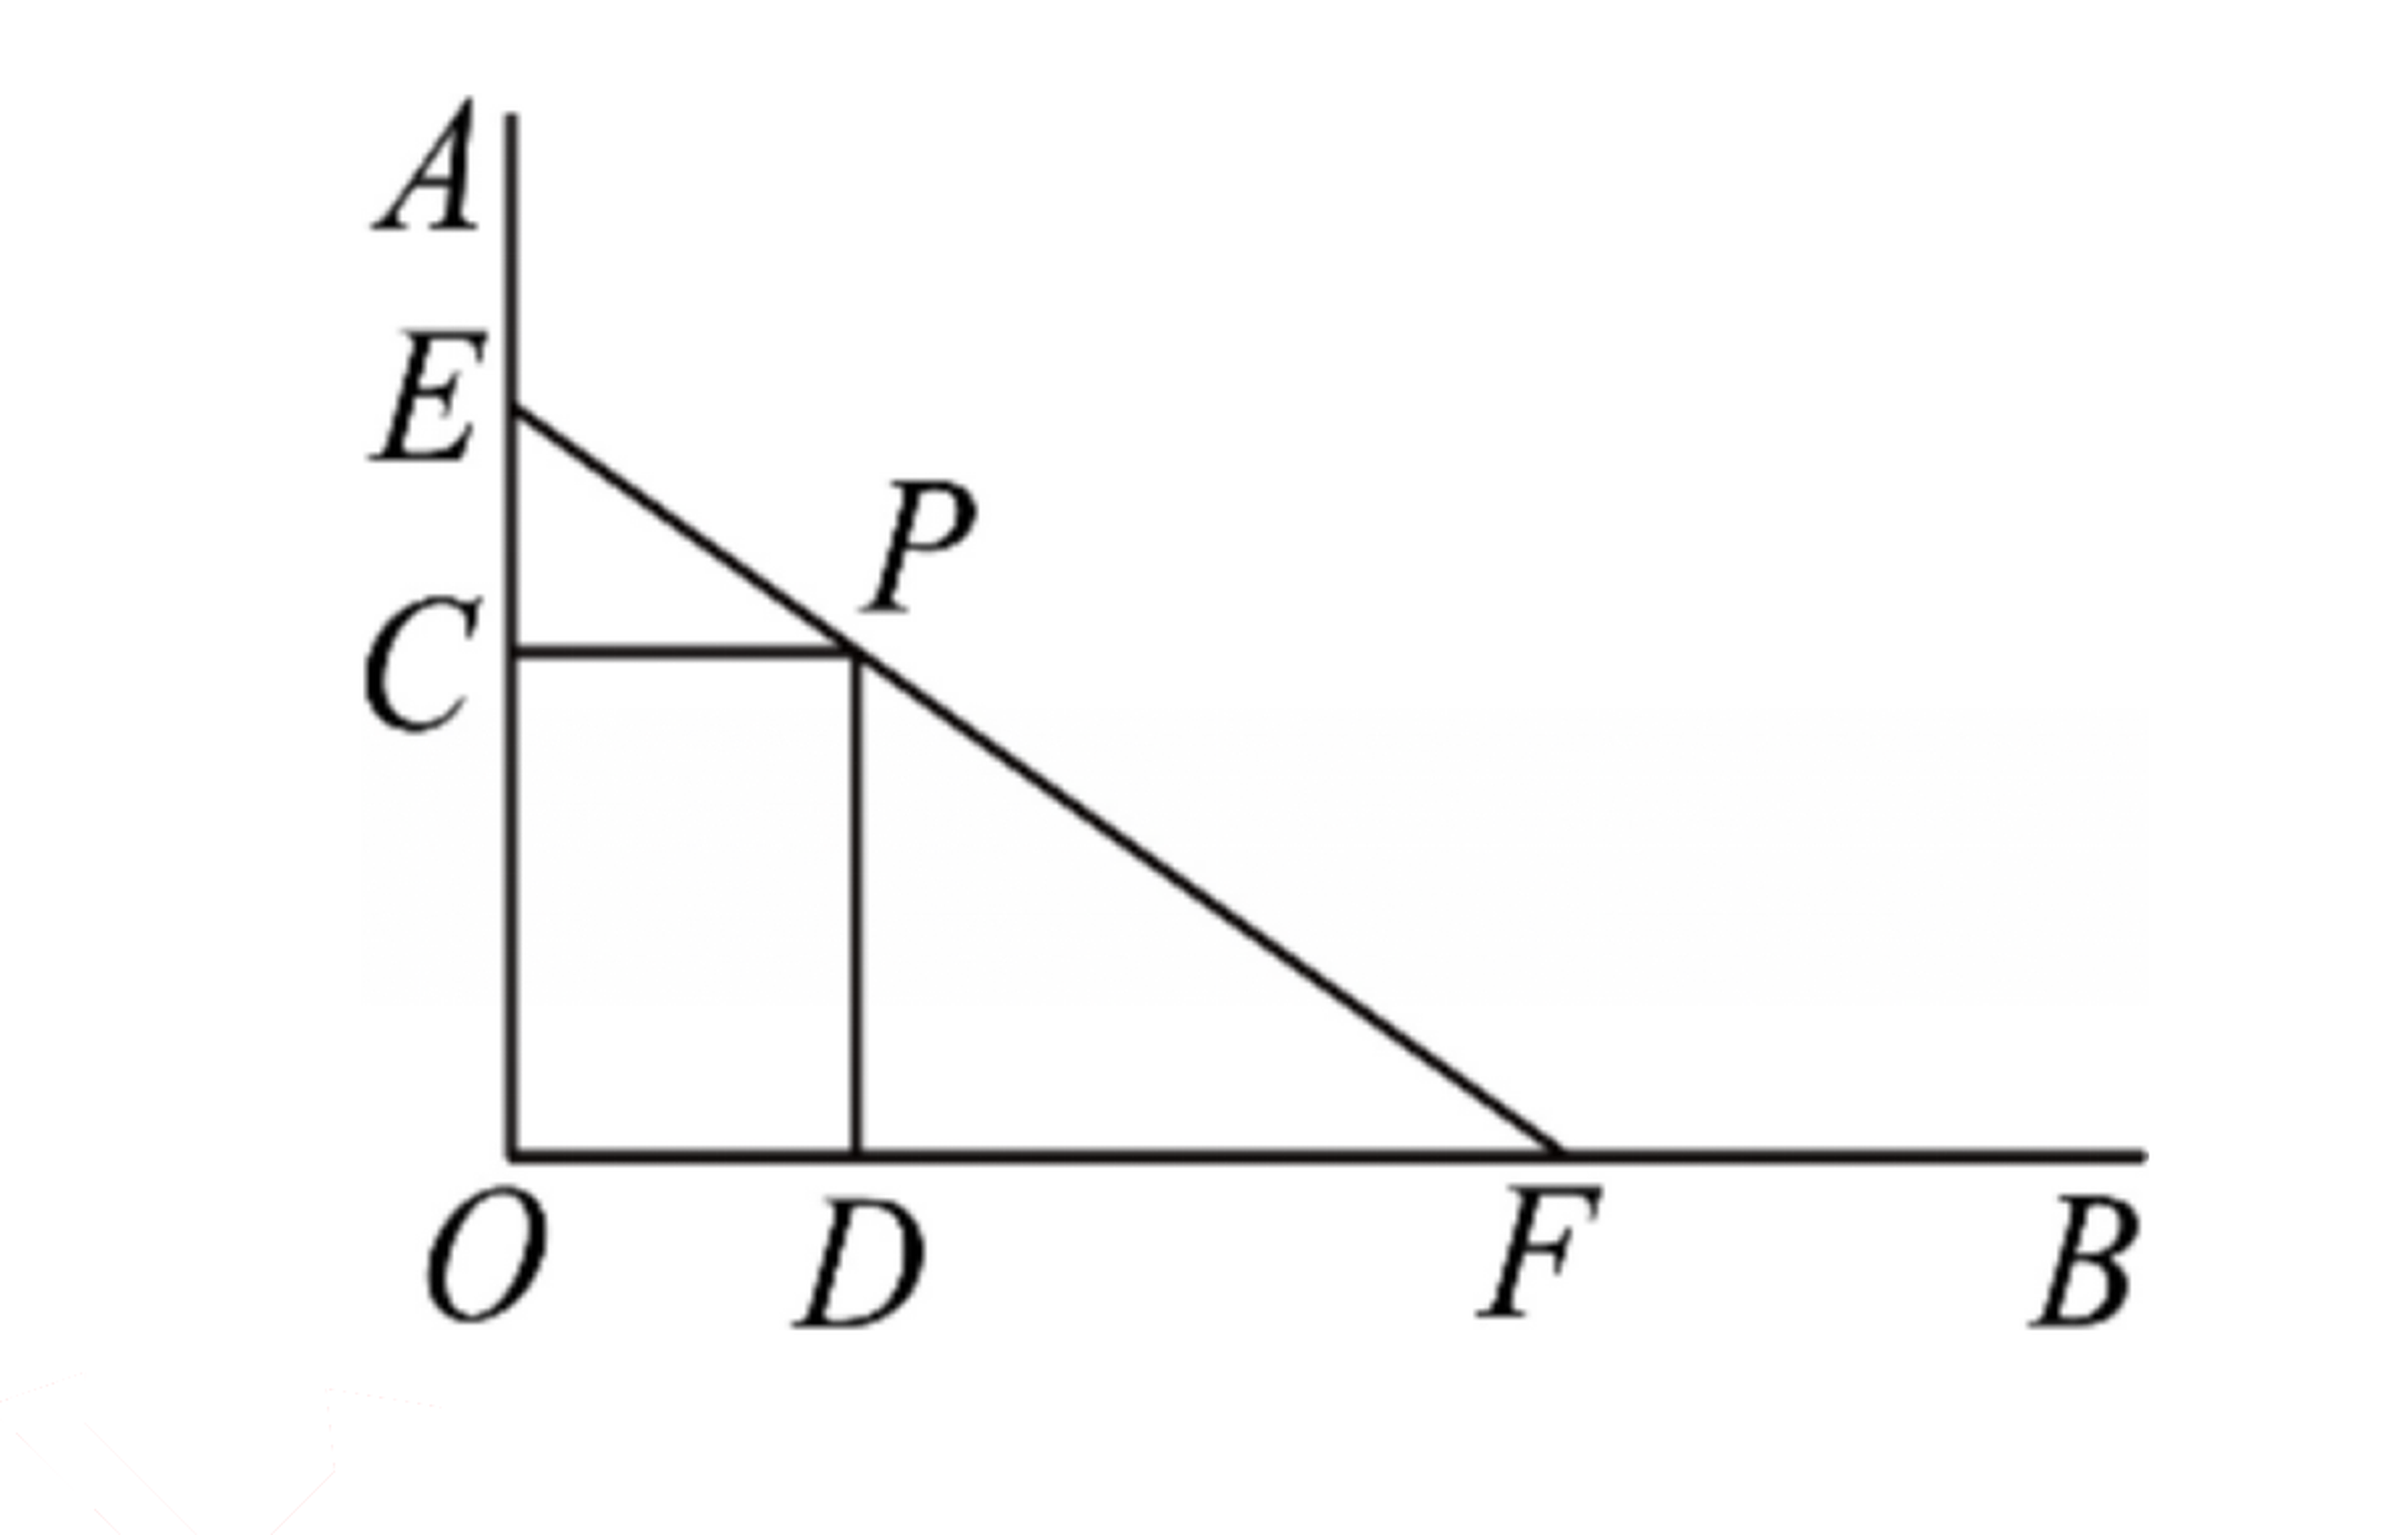
\includegraphics[width=0.32\textwidth]{figures/gao131_q19.png}
\end{center}

\ifanswer
\solbegin
\step{(1) 由题意得 $x\leq60$，}
\step{$\triangle PCE\sim\triangle FDP$，所以 $\dfrac{EC}{CP}=\dfrac{PD}{DF}$，即 $\dfrac{x}{25}=\dfrac{40}{DF}$，得 $DF=\dfrac{1000}{x}$m，}
\step{所以 $OF=OD+DF=\left(25+\dfrac{1000}{x}\right)$m，}
\step{所以 $25+\dfrac{1000}{x}\leq100$，解得 $x\geq\dfrac{40}{3}$；}
\step{综上，$\dfrac{40}{3}\leq x\leq60$；}
\step{(2) 由 $OE=OC+CE=(40+x)$m，}
\step{所以 $S=\dfrac12 OF\cdot OE=\dfrac12\left(25+\dfrac{1000}{x}\right)(40+x)$}
\step{$=\dfrac12\left(1000+25x+\dfrac{40000}{x}+1000\right)$m$^2$，}
\step{由基本不等式得 $S\geq\dfrac12\left(2000+2\sqrt{25x\cdot\dfrac{40000}{x}}\right)=2000$m$^2$，}
\step{当且仅当 $25x=\dfrac{40000}{x}$，即 $x=40$ 时取等号，}
\step{故 $EC=40$m 时，$S$ 取得最小值，为 $2000$m$^2$.}
\solend
\fi

\item 已知 $a\in\R$，函数 $y=ax^2+(3a+2)x+2a+3$.

(1) 当 $a=1$ 时，函数 $y=ax^2+(3a+2)x+2a+3$ 的图象与 $x$ 轴交于 $A(x_1,0)$，$B(x_2,0)$ 两点，求 $x_1^3+x_2^3$；

(2) 若关于 $x$ 的不等式 $ax^2+(3a+2)x+2a+3>2x$ 的解集为 $\R$，求实数 $a$ 的取值范围；

(3) 求关于 $x$ 的不等式 $y\geq1$ 的解集.

\ifanswer
\solbegin
\step{(1) 函数 $y=ax^2+(3a+2)x+2a+3$，当 $a=1$ 时，$y=x^2+5x+5$，}
\step{因为 $y=x^2+5x+5$ 的图象与 $x$ 轴交于 $A(x_1,0)$，$B(x_2,0)$ 两点，}
\step{即 $x^2+5x+5=0$ 的两个根为 $x_1$、$x_2$，}
\step{由根与系数的关系得 $x_1+x_2=-5$，$x_1x_2=5$，}
\step{所以 $x_1^2+x_2^2=(x_1+x_2)^2-2x_1x_2=25-10=15$，}
\step{所以 $x_1^3+x_2^3=(x_1+x_2)(x_1^2+x_2^2-x_1x_2)=-5\times(15-5)=-50$；}
\step{(2) 不等式 $ax^2+(3a+2)x+2a+3>2x$ 恒成立，得 $ax^2+3ax+2a+3>0$.}
\step{当 $a=0$ 时，$3>0$，恒成立，符合题意；}
\step{当 $a\neq0$ 时，若 $a<0$，二次函数 $ax^2+3ax+2a+3$ 开口向下，}
\step{一定存在小于零的部分，故不满足题意；}
\step{当 $a>0$ 时，若使 $ax^2+3ax+2a+3>0$ 恒成立，}
\step{只需 $\Delta=(3a)^2-4\times a\times(2a+3)=a^2-12a<0$，解得 $0<a<12$，}
\step{综上所述，$a$ 的取值范围为 $0\leq a<12$.}
\step{(3) 由 $y\geq1$，得 $ax^2+(3a+2)x+2a+3\geq1$，}
\step{即 $ax^2+(3a+2)x+2a+2\geq0$，即 $(ax+2a+2)(x+1)\geq0$，}
\step{当 $a=0$ 时，$2x+2\geq0$，解得 $x\geq-1$，}
\step{当 $a\neq0$ 时，}
\step{方程 $ax^2+(3a+2)x+2a+2=0$ 即为 $(x+1)(ax+2a+2)=0$，}
\step{解得 $x=-1$ 或 $x=-2-\dfrac2a$，令 $-1=-2-\dfrac2a$，即 $a=-2$，}
\step{当 $a>0$ 时，$-2-\dfrac2a<-1$，}
\step{不等式 $ax^2+(3a+2)x+2a+2\geq0$ 即为 $\left(x+\dfrac{2a+2}a\right)(x+1)\geq0$，}
\step{解得 $x\leq-2-\dfrac2a$ 或 $x\geq-1$；}
\step{当 $a<0$ 时，当 $-2-\dfrac2a<-1$，即 $a<-2$ 时，}
\step{不等式 $ax^2+(3a+2)x+2a+2\geq0$，即为 $\left(x+\dfrac{2a+2}a\right)(x+1)\leq0$，}
\step{解得 $-2-\dfrac2a\leq x\leq-1$；}
\step{当 $-2-\dfrac2a=-1$，即 $a=-2$，}
\step{不等式 $ax^2+(3a+2)x+2a+2\geq0$ 即为 $-2x^2-4x-2\geq0$，解得 $x=-1$，}
\step{当 $-2-\dfrac2a>-1$，即 $-2<a<0$ 时，}
\step{不等式 $ax^2+(3a+2)x+2a+2\geq0$ 即为 $\left(x+\dfrac{2a+2}a\right)(x+1)\leq0$，}
\step{解得 $-1\leq x\leq-2-\dfrac2a$，}
\step{综上所述，当 $a=0$ 时，解集为 $\{x\mid x\geq-1\}$；}
\step{当 $a>0$ 时，解集为 $\{x\mid x\leq-2-\dfrac2a$ 或 $x\geq-1\}$；}
\step{当 $a<-2$ 时，解集为 $\{x\mid -2-\dfrac2a\leq x\leq-1\}$；}
\step{当 $a=-2$ 时，解集为 $\{x\mid x=-1\}$；}
\step{当 $-2<a<0$ 时，解集为 $\{x\mid -1\leq x\leq-2-\dfrac2a\}$.}
\solend
\fi

\item 仔细阅读以下材料：【已知 $a$、$b\in(0,+\infty)$，$a+b=1$，求 $y=\dfrac1a+\dfrac2b$ 的最小值.

$y=\dfrac1a+\dfrac2b=\left(\dfrac1a+\dfrac2b\right)(a+b)=\dfrac ba+\dfrac{2a}b+3\geq3+2\sqrt2$，当且仅当 $\dfrac ba=\dfrac{2a}b$，即 $a=\sqrt2-1$，$b=2-\sqrt2$ 时取得等号，则 $y=\dfrac1a+\dfrac2b$ 的最小值为 $3+2\sqrt2$.

另 $y=\dfrac1a+\dfrac2b=\dfrac{a+b}a+\dfrac{2(a+b)}b=\dfrac ba+\dfrac{2a}b+3\geq3+2\sqrt2$，当且仅当 $\dfrac ba=\dfrac{2a}b$，即 $a=\sqrt2-1$，$b=2-\sqrt2$ 时取得等号，则 $y=\dfrac1a+\dfrac2b$ 的最小值为 $3+2\sqrt2$.】参考上述解法，求解下列问题.

(1) 若正实数 $x$、$y$ 满足 $x+y=1$，求 $\dfrac2x+\dfrac3y$ 的最小值；

(2) 已知 $x\in\left(0,\dfrac12\right)$，求 $t=\dfrac1x+\dfrac8{1-2x}$ 的最小值，并写出此时 $x$ 的值；

(3) 已知 $a$、$b\in(0,+\infty)$，$a+2b=1$，求 $p=\dfrac1{3a+4b}+\dfrac1{a+3b}$ 的最小值.

\ifanswer
\solbegin
\step{(1) 因为 $x>0,y>0$，且 $x+y=1$，}
\step{所以 $\dfrac2x+\dfrac3y=\left(\dfrac2x+\dfrac3y\right)(x+y)=2+\dfrac{2y}x+\dfrac{3x}y+3=5+\dfrac{2y}x+\dfrac{3x}y$，}
\step{由基本不等式得 $\dfrac{2y}x+\dfrac{3x}y\geq2\sqrt{\dfrac{2y}x\cdot\dfrac{3x}y}=2\sqrt6$，}
\step{当且仅当 $\dfrac{2y}x=\dfrac{3x}y$，即 $2y^2=3x^2$ 时，等号成立，}
\step{又因为 $x>0,y>0$ 且 $x+y=1$，此时 $x=\sqrt6-2,y=3-\sqrt6$，}
\step{所以 $\dfrac2x+\dfrac3y\geq5+2\sqrt6$，故 $\dfrac2x+\dfrac3y$ 的最小值为 $5+2\sqrt6$.}
\step{(2) 由 $0<x<\dfrac12$，则 $t=\dfrac1x+\dfrac8{1-2x}=\dfrac{2(1-2x+2x)}{2x}+\dfrac{8(1-2x+2x)}{1-2x}$}
\step{$=10+\dfrac{2\cdot(1-2x)}{2x}+\dfrac{8\cdot2x}{1-2x}\geq10+2\sqrt{\dfrac{2\cdot(1-2x)}{2x}\cdot\dfrac{8\cdot2x}{1-2x}}=18$，}
\step{当且仅当 $\dfrac{2\cdot(1-2x)}{2x}=\dfrac{8\cdot2x}{1-2x}$，即 $x=\dfrac16$ 时等号成立；}
\step{(3) 由 $a$、$b>0$，$a+2b=1$，则 $a=1-2b>0$，即 $0<b<\dfrac12$，}
\step{所以 $p=\dfrac1{3a+4b}+\dfrac1{a+3b}=\dfrac1{3a+6b-2b}+\dfrac1{a+2b+b}=\dfrac1{3-2b}+\dfrac1{1+b}$}
\step{$=\dfrac1{3-2b}+\dfrac2{2+2b}$，显然 $3-2b$、$2+2b>0$，}
\step{所以 $p=\dfrac15\cdot(3-2b+2+2b)\cdot\left(\dfrac1{3-2b}+\dfrac2{2+2b}\right)=\dfrac15\left[3+\dfrac{2+2b}{3-2b}+\dfrac{2(3-2b)}{2+2b}\right]$}
\step{$\geq\dfrac15\left[3+2\sqrt{\dfrac{2+2b}{3-2b}\cdot\dfrac{2(3-2b)}{2+2b}}\right]=\dfrac{3+2\sqrt2}5$，}
\step{当且仅当 $\dfrac{2+2b}{3-2b}=\dfrac{2(3-2b)}{2+2b}$，}
\step{即 $b=\dfrac{8-5\sqrt2}2$，$a=5\sqrt2-7$ 时等号成立.}
\solend
\fi

\end{enumerate}

\end{document}
"
% 紧凑版：xelatex "\def\iscompact{1}% 高一131_六十中学_期中.tex
%   —— 高一上数学"2026-2027 年六十中学高一上期中"（试卷版/答案版）
% 试卷版：xelatex 高一131_六十中学_期中.tex
% 答案版：xelatex "\def\isanswer{1}\input{高一131_六十中学_期中.tex}"
% 紧凑版：xelatex "\def\iscompact{1}\input{高一131_六十中学_期中.tex}"
%
% 原始材料：微信公众号"魔都数学加油站"文章，作者破晓，2026-11-13 18:18 发布；
% 连载"27学年高一131"，原文标题"27学年高一131——2026-2027年上海市六十中学高一上期中"；
% 原文链接：https://mp.weixin.qq.com/s/Nrbp3Uvt-sOGnOp4MEHemA。
% 正文为 11 张 PNG 页（01—05、09—11 为 2560x3620，06—08 为 4762x6735），
% 题目下印有【解析】或【答案】，为讲评版。题目、解析均据原图转录；
% 卷面粉红色水印"魔都数学加油站"及公众号页脚未录入。全卷仅第 19 题有 1 幅插图
% （矩形 OCPD 与小路 EF 的示意图），取 07.png 截图去水印。
%
% 卷首标题：原卷印作"2026-2027 年六十中学高一上期中"（公众号标题中的"上海市"
% 卷面标题行没有，本稿照卷面），年份区间按全稿惯例排 en dash；原卷未印副标题，
% 本卷为期中卷、跨集合与常用逻辑用语／不等式／函数三章，按题目内容标为
% "集合与常用逻辑用语、不等式、函数"（与 125／126／128／129 同期中卷口径相同）：
% 集合与逻辑见 Q3、Q4、Q7、Q13、Q17，不等式见 Q8、Q10、Q12、Q14、Q15、Q16、Q19、
% Q20、Q21，函数（指数／对数／幂函数、基本不等式应用）见 Q5、Q6、Q9、Q11、Q18、Q21。
%
% 题号体例：本卷共 19 题——一、填空题 3—12（10 题）、二、选择题 13—16（4 题）、
% 三、解答题 17—21（5 题）。三节分别 \setcounter{enumi}{2}／{12}／{16}。
%
% 与原卷的排版差异：
%   ① 原文从第 3 题起，本稿保留原题号（见上"题号体例"）；
%   ② 原卷每题下直接印【解析】／【答案】，本稿按全稿惯例置于答案版；第 3、4 题只印
%      【答案】，另提 \ans{}；第 13—16 题答案在解析末句"故选 …"，题干括号内留空、
%      不另提 \ans{}；其余各题印【解析】、无独立答案段；
%   ③ 原卷未印副标题，本稿按"知识模块"口径补出；
%   ④ 原卷填空横线按全稿惯例排为 \blankline[4.4em]；选择题括号排 \mbox{（\quad）}、
%      选项段前按惯例加 \keepwithprev；解答题不留作答区（原卷为讲评版，与 109—129 同）；
%   ⑤ 原卷数集排斜体 $R$／$N$，按全稿惯例改 \R／\N；绝对值排 \lvert…\rvert，
%      集合描述竖线排 \mid；不等号按全稿惯例排 \leqslant／\geqslant；
%   ⑥ 子题标号 (1)(2)(3) 原卷用半角括号，照录；圈数字 ①② 照录；
%   ⑦ 原卷第 19 题插图浮排在第 07 页题干右侧，本稿按体例就近置于题干"如图"之后
%      （居中 \includegraphics），图取原卷 07 页截图去水印；题前按惯例加
%      \needvspace{7cm} 守卫（照 高一120／127／129 成例），保证"题干 + 图"整块不被页边界切开；
%   ⑧ 原卷 Q9 题干跨 01—02 页、Q15 解析跨 03—04 页、Q16 材料跨 04—05 页、
%      Q17 题干跨 05—06 页、Q20 解析跨 08—09 页、Q21 解析跨 09—11 页，
%      本稿按题合并连续排版；末页第 11 页为 Q21 (3) 解析的续尾，按实际印刷行单列。
%   ⑨ 第 16 题材料英文括注原卷印作 (Cauchy – SchwarzInequality)（长横、Schwarz 与
%      Inequality 斜体连排无空格），本稿按全稿英文专名惯例排 \emph{(Cauchy-Schwarz Inequality)}；
%      第 15 题解析 B、D 两行原卷各印一步含 \lg m 的换底繁分数（2026-11-13 回原图核对补回，
%      本稿初转曾顺手去重跳过该步）。
%
% 判别式字形：第 20 题 (2) 解析 $\Delta=(3a)^2-4\times a\times(2a+3)=a^2-12a<0$
%   原卷排三角形（等腰、高；回 08.png 放大核对），照录 \Delta；全卷判别式仅此一处
%   （\triangle 另作第 19 题「$\triangle PCE\sim\triangle FDP$」的几何三角形记号）。
%
% 子集符号：第 17 题 (2) 解析 $P\subseteq Q$ 印带下划线，照录 \subseteq；
%   全卷未出现单线 \subset。
%
% 原卷存疑照录：
%   第 11 题解析末两式作 $\dfrac{2+m+\frac1n}{2n+2}=\dfrac{2n+mn+1}{2n+2}$，而第三式
%     分母 $\log_3 9+\log_3 2+\log_3 2=2+\frac2n$，与前一分母 $2n+2$ 不等，照录；
%   第 16 题材料 ①"对于所有实数 $x$ 和 $y$，有 $(a^2+b^2)(c^2+d^2)\geq(ac+bd)^2$"
%     句首用 $x$、$y$ 而式中用 $a$、$b$、$c$、$d$，照录；
%   第 20 题题干 (2) 作"解集为 $\R$"、解析 (2) 作"恒成立"，措辞不同，照录；
%   第 21 题材料把同一道题用两种解法连印两遍（"另 $y=\frac1a+\frac2b=\dots$"），照录；
%   第 21 题 (3) 解析末句"即 $b=\frac{8-5\sqrt2}{2}$，$a=5\sqrt2-7$ 时等号成立"
%     未另写"故最小值为 $\frac{3+2\sqrt2}{5}$"，照录；
%   第 12 题解析"所以 $e^a+e^b>e^c, a+b>c$"、第 8 题解析"$a>0$，$b>0$"、
%     第 18 题 (2)"$4x^2-4x+1<x^2+4x+4$，解得 $-\frac13<x<3$"等处数学式内
%     半角逗号，照录；
%   第 15 题解析用 $\lg$ 记常用对数（$\lg m$、$\lg 3$、$\lg 5$、$\lg 15$），照录。
%
% 行数复核：逐题数 \step 条数，合计 119 条（Q3：0；Q4：0；Q5：1；Q6：1；Q7：2；
% Q8：2；Q9：1；Q10：1；Q11：2；Q12：6；Q13：2；Q14：3；Q15：14；Q16：10；
% Q17：4；Q18：8；Q19：11；Q20：35；Q21：16），与原卷印刷行逐题相等
% （cases 块作一个印刷行计）。第 3、4 题只印【答案】，提 \ans{}，不计入 \step 账；
% 四道选择题答案均在解析末句，括号内留空、不另提 \ans{}。
%
\documentclass[a4paper,11pt]{article}
\usepackage{common}

\begin{document}

\examtitlest[3]{2026--2027 年六十中学高一上期中}{集合与常用逻辑用语、不等式、函数}

\bigsec{一、填空题}

\begin{enumerate}
\setcounter{enumi}{2}

\item 已知集合 $A=(0,4),B=[2,5]$，则 $A\cup B=$\blankline[4.4em].

\ifanswer
\ans{$(0,5]$}
\fi

\item 陈述句“$x=2$ 或 $y=3$”的否定形式为\blankline[4.4em].

\ifanswer
\ans{$x\neq2$ 且 $y\neq3$}
\fi

\item 函数 $y=a^{x-2}+15(a>0$ 且 $a\neq1)$ 的图象恒过定点的坐标为\blankline[4.4em].

\ifanswer
\solbegin
\step{函数 $y=a^{x-2}+15$ 的图象恒过定点 $A(2,16)$.}
\solend
\fi

\item 用有理数指数幂的形式来化简：$\dfrac{\sqrt{a\cdot\sqrt[3]{a^4}}}{\left(a^{\frac13}\right)^2}=$\blankline[4.4em].

\ifanswer
\solbegin
\step{原式 $=\dfrac{\sqrt{a\cdot a^{\frac43}}}{a^{\frac23}}=\dfrac{\sqrt{a^{\frac73}}}{a^{\frac23}}=\dfrac{a^{\frac76}}{a^{\frac23}}=a^{\frac76-\frac23}=a^{\frac12}(a>0)$.}
\solend
\fi

\item 已知集合 $A=\left\{x\mid \dfrac6{6-x}\in\N\text{ 且 }x\in\N\right\}$，则用列举法表示集合 $A=$\blankline[4.4em].

\ifanswer
\solbegin
\step{当 $x=0$ 时，$\dfrac6{6-0}=1\in\N$，当 $x=3$ 时，$\dfrac6{6-3}=2\in\N$，}
\step{当 $x=4$ 时，$\dfrac6{6-4}=3\in\N$，当 $x=5$ 时，$\dfrac6{6-5}=6\in\N$，故 $A=\{0,3,4,5\}$.}
\solend
\fi

\item 已知 $a>0$，$b>0$，且 $ab=\dfrac12$，则 $\dfrac1a+\dfrac8b$ 的最小值是\blankline[4.4em].

\ifanswer
\solbegin
\step{$a>0$，$b>0$，且 $ab=\dfrac12$，则 $\dfrac1a+\dfrac8b\geq2\sqrt{\dfrac8{ab}}=8$，}
\step{当且仅当 $\dfrac1a=\dfrac8b$，即 $a=\dfrac14,b=2$ 时取等号，故最小值为 $8$.}
\solend
\fi

\item 心理学家有时用函数 $L(t)=A(1-e^{-kt})$ 测定在时间 $t$（单位：$min$）内能够记忆的量 $L$，其中 $A$ 表示需要记忆的量，$k$ 表示记忆率. 假设一个学生需要记忆的量为 $200$ 个单词，此时 $L$ 表示在时间 $t$ 内该生能够记忆的单词个数. 已知该生在 $5min$ 内能够记忆 $20$ 个单词，则 $k$ 的值约为\blankline[4.4em]（结果保留四位小数）.

\ifanswer
\solbegin
\step{由题意得 $200(1-e^{-5k})=20$，所以 $e^{-5k}=0.9$，解得 $k\approx0.0211$.}
\solend
\fi

\item 设 $x\in\R$，方程 $\lvert 3x-2\rvert+\lvert 1-x\rvert=\lvert 2x-1\rvert$ 的解集是\blankline[4.4em].

\ifanswer
\solbegin
\step{由三角不等式得 $(3x-2)(1-x)\geq0$，故解集是 $\left[\dfrac23,1\right]$.}
\solend
\fi

\item 已知 $3^m=5$，$n=\log_2 3$，则 $\log_{36}90$ 可用 $m$、$n$ 表示为\blankline[4.4em].

\ifanswer
\solbegin
\step{由 $3^m=5$，又 $n=\log_2 3$，得 $m=\log_3 5$，$\log_3 2=\dfrac{\log_2 2}{\log_2 3}=\dfrac1n$，}
\step{所以 $\log_{36}90=\dfrac{\log_3 90}{\log_3 36}=\dfrac{\log_3 9+\log_3 2+\log_3 5}{\log_3 9+\log_3 2+\log_3 2}=\dfrac{2+m+\frac1n}{2n+2}=\dfrac{2n+mn+1}{2n+2}$.}
\solend
\fi

\item 若定义域为 $I=(0,m]$ 的函数 $f(x)=e^x$ 满足：对任意能构成三角形三边长的实数 $a$、$b$、$c\in I$，均有 $f(a)$、$f(b)$、$f(c)$ 也能构成三角形三边长，则 $m$ 的最大值为\blankline[4.4em].

\ifanswer
\solbegin
\step{$f(x)=e^x$ 在 $I=(0,m]$ 上严格增，所以 $f(x)\in(1,e^m]$，不妨设 $0<a\leq b\leq c$，}
\step{因为对任意能构成三角形三边长的实数 $a,b,c\in I$，均有 $f(a)$，$f(b)$，$f(c)$}
\step{也能构成三角形三边长，所以 $e^a+e^b>e^c, a+b>c$，}
\step{因为 $e^a+e^b\geq2\sqrt{e^ae^b}=2\sqrt{e^{a+b}}>e^c$，所以 $4e^{a+b}>e^{2c}$，}
\step{因为对任意 $a,b,c\in I$ 都成立，所以 $4e^c\geq e^{2c}$，所以 $e^c\leq4$，所以 $c\leq\ln4$，}
\step{所以 $m\leq\ln4$，所以 $m$ 的最大值为 $\ln4$.}
\solend
\fi

\end{enumerate}

\bigsec{二、选择题}

\begin{enumerate}
\setcounter{enumi}{12}

\item 已知 $m,n$ 是非零自然数，命题 $\alpha:mn$ 是奇数，命题 $\beta:m$ 或 $n$ 是奇数，则 $\alpha$ 是 $\beta$ 的\mbox{（\quad）}

\keepwithprev
A. 充分非必要条件\qquad\qquad B. 必要非充分条件

C. 充要条件\qquad\qquad D. 既非充分又非必要条件

\ifanswer
\solbegin
\step{$mn$ 是奇数 $\Leftrightarrow$ $m$、$n$ 都是奇数，所以 $\alpha$ 能推出 $\beta$，充分性成立，}
\step{但 $\beta$ 推不出 $\alpha$，必要性不成立，所以 $\alpha$ 是 $\beta$ 的充分非必要条件. 故选 $A$.}
\solend
\fi

\item 关于 $x$ 的不等式 $x^2-mx+n+5\leq0$ 的解集是 $[1,8]$，那么 $\log_m n=$\mbox{（\quad）}

\keepwithprev
A. $\dfrac13$\qquad\qquad B. $-3$\qquad\qquad C. $-2$\qquad\qquad D. $\dfrac12$

\ifanswer
\solbegin
\step{由题意得 $x^2-mx+n+5=0$ 的解为 $1$，$8$，}
\step{由根与系数的关系得 $\begin{cases}1+8=m\\1\times8=n+5\end{cases}$，解得 $m=9$，$n=3$，}
\step{所以 $\log_m n=\log_9 3=\dfrac12\log_3 3=\dfrac12$. 故选 $D$.}
\solend
\fi

\item 已知正实数 $x$、$y$、$z$ 满足 $3^x=5^y=15^z$，则下列说法中不正确的是\mbox{（\quad）}

\keepwithprev
A. $\dfrac1x+\dfrac1y=\dfrac1z$\qquad\qquad B. $x+y>2z$\qquad\qquad C. $3x>5y>15z$\qquad\qquad D. $x\cdot y>4z^2$

\ifanswer
\solbegin
\step{已知正实数 $x$、$y$、$z$，则设 $3^x=5^y=15^z=m>1$，}
\step{所以 $x=\log_3 m$，$y=\log_5 m$，$z=\log_{15} m$，}
\step{对于 $A$，$\dfrac1x+\dfrac1y=\dfrac1{\log_3 m}+\dfrac1{\log_5 m}=\log_m 3+\log_m 5=\log_m 15=\dfrac1z$，故 $A$ 正确；}
\step{对于 $B$，因为 $\dfrac{x+y}{z}=\dfrac{x}{z}+\dfrac{y}{z}=\dfrac{\log_3 m}{\log_{15} m}+\dfrac{\log_5 m}{\log_{15} m}=\dfrac{\dfrac{\lg m}{\lg3}}{\dfrac{\lg m}{\lg15}}+\dfrac{\dfrac{\lg m}{\lg5}}{\dfrac{\lg m}{\lg15}}=\dfrac{\lg15}{\lg3}+\dfrac{\lg15}{\lg5}$，}
\step{$=\dfrac{\lg3+\lg5}{\lg3}+\dfrac{\lg3+\lg5}{\lg5}=2+\dfrac{\lg5}{\lg3}+\dfrac{\lg3}{\lg5}=2+\log_3 5+\log_5 3$，}
\step{又 $\log_3 5>0$，$\log_5 3>0$，所以 $2+\log_3 5+\log_5 3>2$，}
\step{所以 $\dfrac{x+y}{z}>2$，即 $x+y>2z$，故 $B$ 正确；}
\step{对于 $C$，因为 $\dfrac5x=5\log_m 3=\log_m 243$，$\dfrac3y=3\log_m 5=\log_m 125$，}
\step{所以 $\dfrac5x>\dfrac3y$，即 $3x<5y$，故 $C$ 错误；}
\step{对于 $D$，$\dfrac{xy}{z^2}=\dfrac{x}{z}\cdot\dfrac{y}{z}=\dfrac{\log_3 m}{\log_{15} m}\cdot\dfrac{\log_5 m}{\log_{15} m}=\dfrac{\dfrac{\lg m}{\lg3}}{\dfrac{\lg m}{\lg15}}\cdot\dfrac{\dfrac{\lg m}{\lg5}}{\dfrac{\lg m}{\lg15}}=\dfrac{\lg15}{\lg3}\cdot\dfrac{\lg15}{\lg5}$}
\step{$=\dfrac{\lg3+\lg5}{\lg3}\cdot\dfrac{\lg3+\lg5}{\lg5}=\left(1+\dfrac{\lg5}{\lg3}\right)\left(1+\dfrac{\lg3}{\lg5}\right)=2+\dfrac{\lg5}{\lg3}+\dfrac{\lg3}{\lg5}$}
\step{$\geq2+2\sqrt{\dfrac{\lg5}{\lg3}\cdot\dfrac{\lg3}{\lg5}}=2+2=4$，又 $\lg3\neq\lg5$，故等号不成立，}
\step{所以 $\dfrac{xy}{z^2}>4$，即 $xy>4z^2$，故 $D$ 正确.}
\step{故选 $C$.}
\solend
\fi

\item 柯西不等式 \emph{(Cauchy-Schwarz Inequality)} 是一种在数学和物理学中广泛使用的不等式，它是由法国数学家奥古斯丁$\cdot$路易$\cdot$柯西提出的，柯西不等式可以用于证明其他不等式，也可以用于解决一些数学问题. 以下是柯西不等式的原始形式：

①对于所有实数 $x$ 和 $y$，有 $(a^2+b^2)(c^2+d^2)\geq(ac+bd)^2$.

②等式条件：当且仅当 $ad-bc=0$ 时，等号成立.

例：已知 $x+2y=2$，由柯西不等式 $(x^2+y^2)(1^2+2^2)\geq(x+2y)^2$，可得 $(x^2+y^2)_{min}=\dfrac45$.

现给出以下两个命题：

①若 $a^2+b^2=1$，则 $2a+3b$ 的最大值为 $\sqrt{13}$；

②若 $1<a<3$，则 $\sqrt{a-1}+\sqrt{6-2a}$ 的最大值为 $\sqrt6$；

则运用柯西不等式，判断以下正确的选项有\mbox{（\quad）}

\keepwithprev
A. ①为真命题；②为真命题\qquad\qquad B. ①为真命题；②为假命题

C. ①为假命题；②为真命题\qquad\qquad D. ①为假命题；②为假命题

\ifanswer
\solbegin
\step{由柯西不等式得 $(a^2+b^2)(2^2+3^2)\geq(2a+3b)^2$.}
\step{因为 $a^2+b^2=1$，所以 $(2^2+3^2)\geq(2a+3b)^2$，即 $13\geq(2a+3b)^2$，}
\step{所以 $-\sqrt{13}\leq2a+3b\leq\sqrt{13}$，则 $(2a+3b)_{max}=\sqrt{13}$，}
\step{当且仅当 $3a=2b$ 时取等号，故①正确.}
\step{令 $x=\sqrt{a-1}$，$y=\sqrt{3-a}$，则 $x^2+y^2=a-1+3-a=2$，}
\step{由柯西不等式得 $(\sqrt{a-1}+\sqrt{6-2a})^2=(\sqrt{a-1}+\sqrt2\cdot\sqrt{3-a})^2=(x+\sqrt2 y)^2$}
\step{$\leq[1^2+(\sqrt2)^2](x^2+y^2)$，}
\step{因为 $x^2+y^2=2$，所以 $(\sqrt{a-1}+\sqrt{6-2a})^2\leq6$，}
\step{当且仅当 $\sqrt{3-a}=\sqrt2\sqrt{a-1}$ 取等号，所以 $\sqrt{a-1}+\sqrt{6-2a}\leq\sqrt6$，故②正确.}
\step{故选 $A$.}
\solend
\fi

\end{enumerate}

\bigsec{三、解答题}

\begin{enumerate}
\setcounter{enumi}{16}

\item 已知集合 $P=\left\{x\mid \dfrac{3x-1}{x+2}<1\right\}$，集合 $Q=\{x\mid\lvert x-a\rvert\leq2\}$.

(1) 求集合 $P$；

(2) 若“$x\in P$”是“$x\in Q$”的充分非必要条件，求实数 $a$ 的取值范围.

\ifanswer
\solbegin
\step{(1) 集合 $P=\left\{x\mid \dfrac{3x-1}{x+2}<1\right\}$，得 $\dfrac{2x-3}{x+2}<0$，解得 $P=\left(-2,\dfrac32\right)$.}
\step{(2) 集合 $Q=\{x\mid\lvert x-a\rvert\leq2\}=\{x\mid a-2\leq x\leq2+a\}$，}
\step{由“$x\in P$”是“$x\in Q$”的充分非必要条件，得 $P\subseteq Q$，}
\step{得 $\begin{cases}-2\geq a-2\\\dfrac32\leq2+a\\a-2<2+a\end{cases}$，解得 $a\in\left[-\dfrac12,0\right]$.}
\solend
\fi

\item 已知幂函数 $f(x)=(m^2-4m+4)\cdot x^{2m-4}$ 在 $(-\infty,0)$ 上是严格减函数.

(1) 求函数 $y=f(x)$ 的解析式；

(2) 若 $f(1-2x)<f(x+2)$，求 $x$ 的取值范围.

\ifanswer
\solbegin
\step{(1) 由幂函数的定义得 $m^2-4m+4=1$，解得 $m=1$ 或 $3$，}
\step{当 $m=1$ 时，$f(x)=x^{-2}=\dfrac1{x^2}$，在 $(-\infty,0)$ 上严格增，不符合题意，}
\step{当 $m=3$ 时，$f(x)=x^2$，在 $(-\infty,0)$ 上严格减，符合题意，}
\step{所以 $f(x)=x^2$；}
\step{(2) 由函数 $f(x)=x^2$ 图象关于 $y$ 轴对称，且在 $[0,+\infty)$ 上严格增，}
\step{则 $f(1-2x)<f(x+2)$ 可化为 $\lvert1-2x\rvert<\lvert x+2\rvert$，}
\step{平方得 $4x^2-4x+1<x^2+4x+4$，解得 $-\dfrac13<x<3$，}
\step{所以 $x$ 的取值范围是 $\left(-\dfrac13,3\right)$.}
\solend
\fi

% 第 19 题是"题干 + 图"约 7cm 的一整块，守卫放在 \item 之前（放 \item 之后会失效）
\needvspace{7cm}
\item 如图，$OA$、$OB$ 是两条长度足够长的互相垂直的笔直小路，矩形 $OCPD$ 的顶点 $C$，$D$ 分别在 $OA$、$OB$ 上，且该矩形区域内种满了荷花. 为了让观赏者有更好的观赏体验，现计划经过点 $P$ 修一条小路 $EF$，其中点 $E$ 在小路 $OA$ 上，点 $F$ 在小路 $OB$ 上，并在 $\triangle OEF$ 区域内种满荷花. 已知 $OD=25m$，$OC=40m$，且小路 $EF$ 要完全位于一个以 $O$ 为顶点的，边长为 $100$ m 的正方形内部（包括边界）. 记 $\triangle OEF$ 的面积为 $S$m$^2$.

(1) 设 $EC=x\cdot m$，试用 $x$ 表示 $OF$，并求 $x$ 的取值范围.

(2) 当 $EC$ 的长度为多少时，$S$ 取得最小值？最小值是多少？

\begin{center}
% 图取原卷 07.png 截图去粉色水印，2.8× LANCZOS 放大
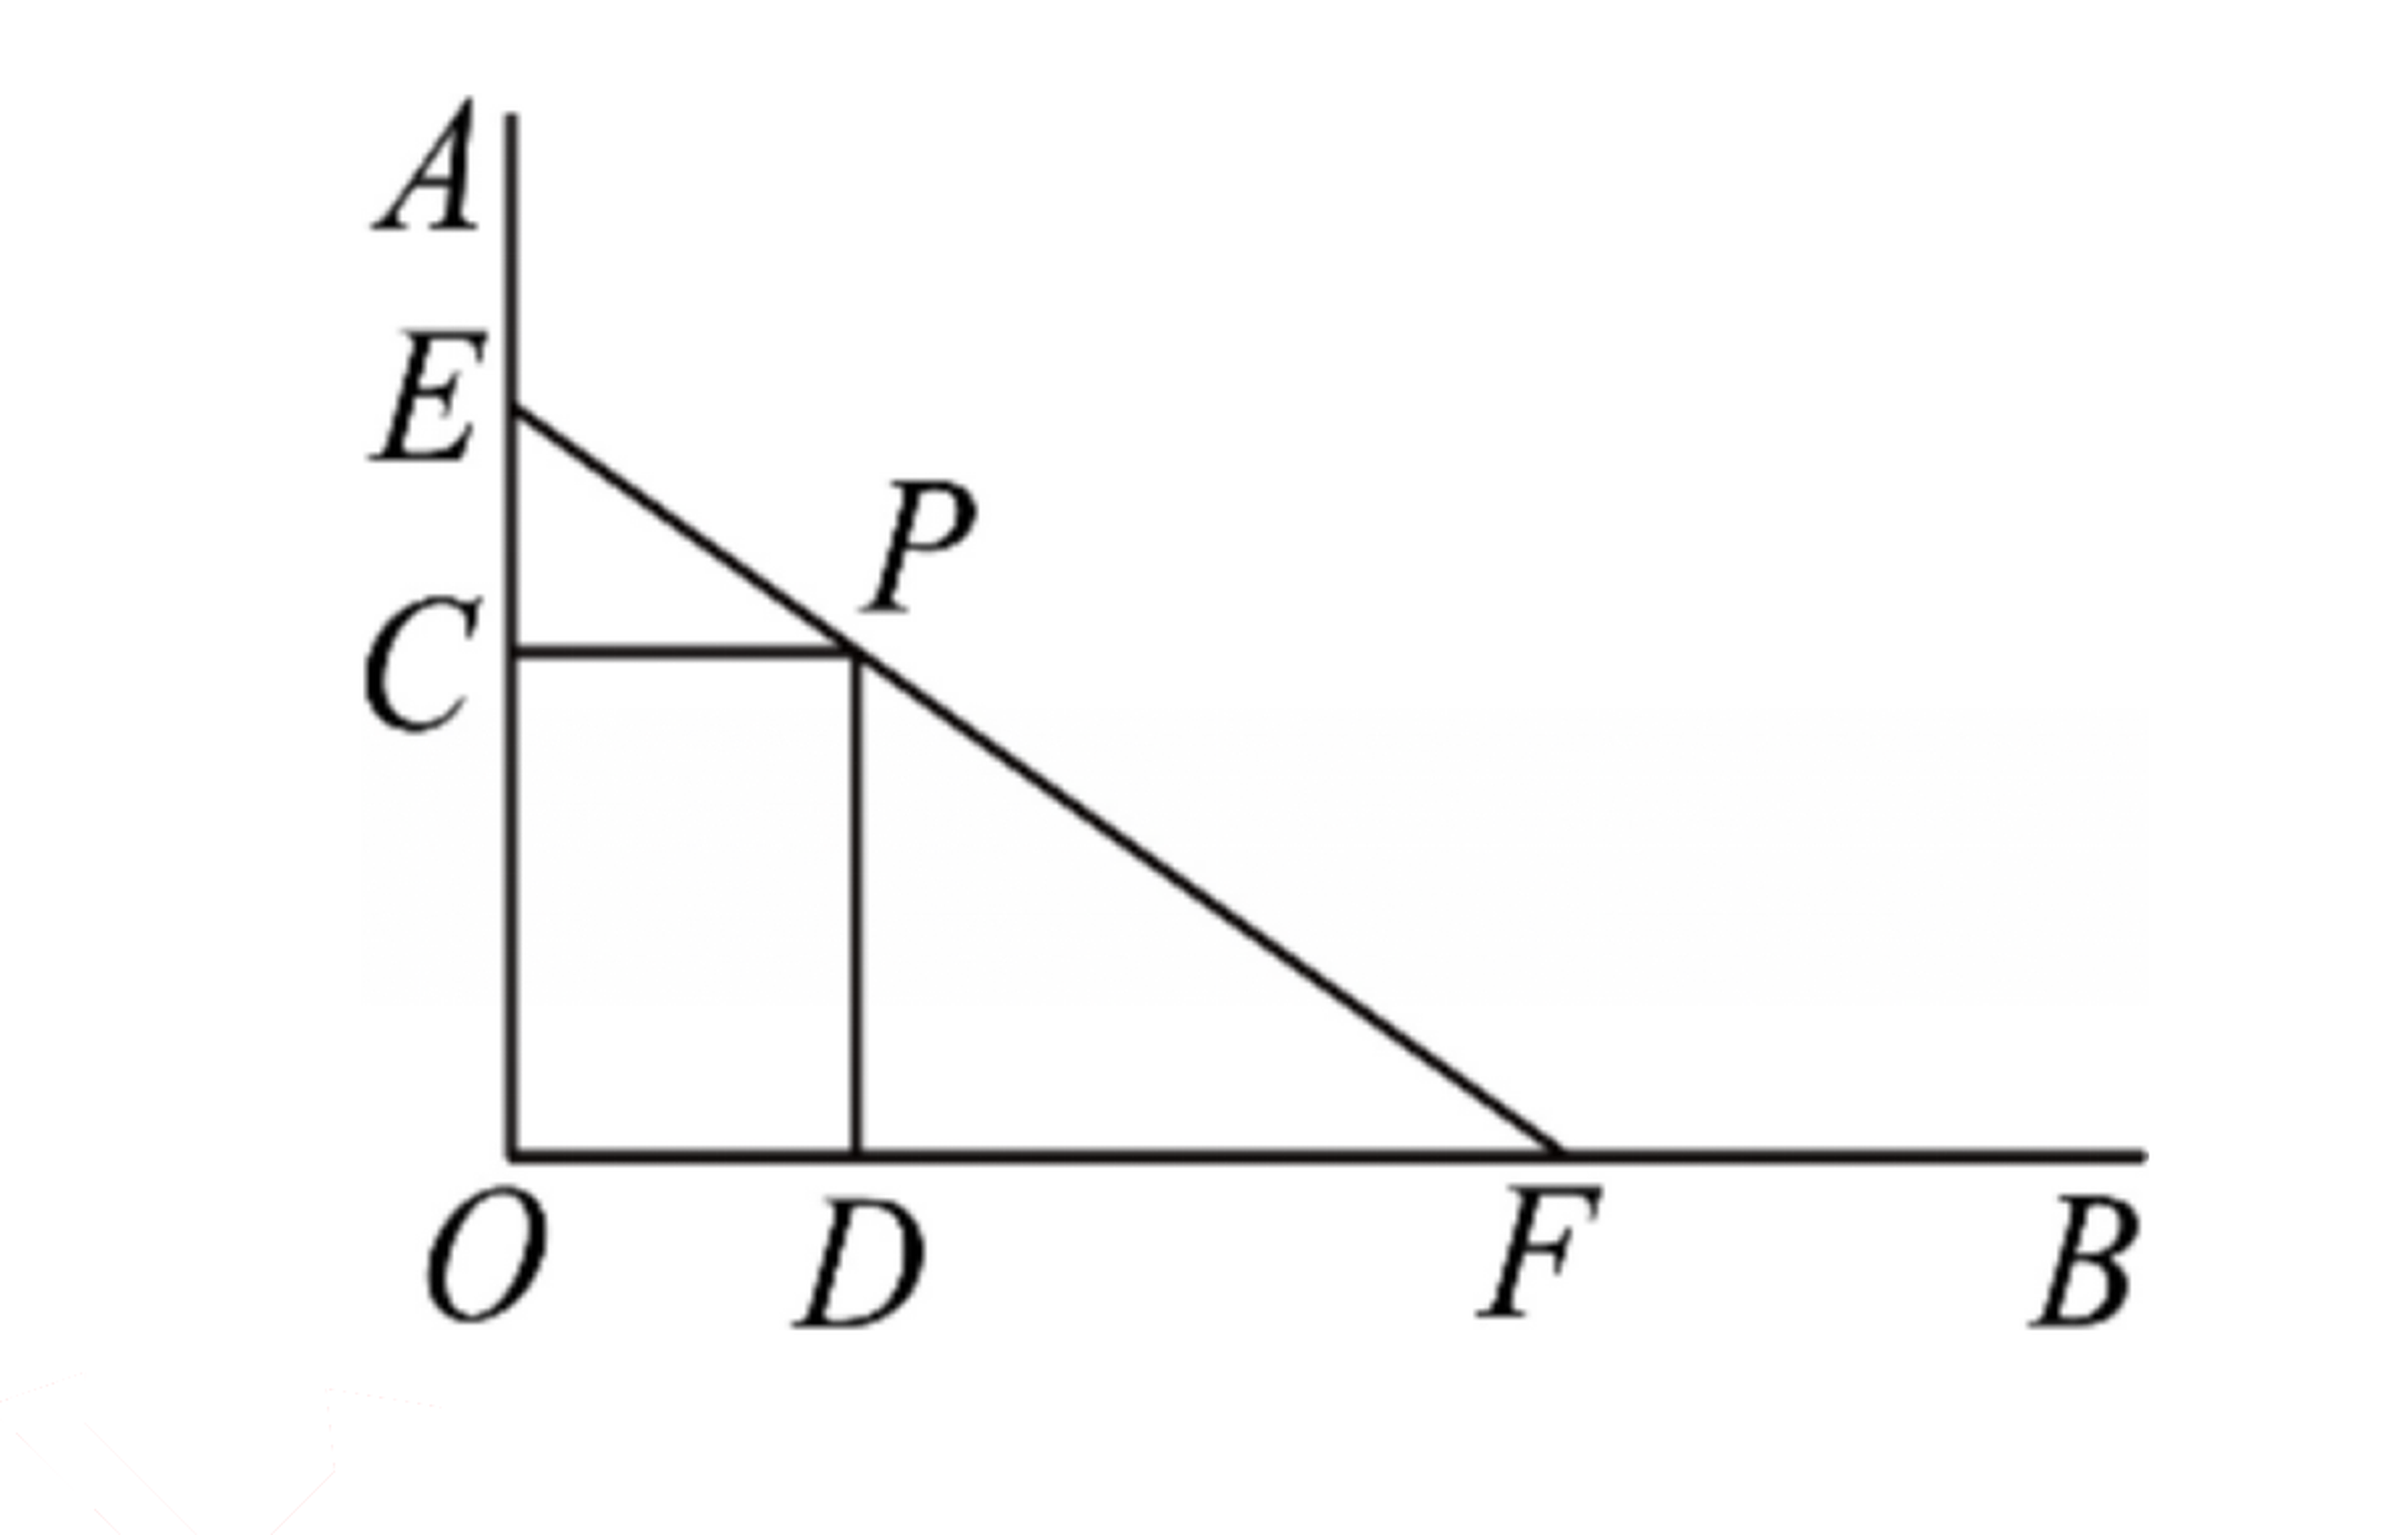
\includegraphics[width=0.32\textwidth]{figures/gao131_q19.png}
\end{center}

\ifanswer
\solbegin
\step{(1) 由题意得 $x\leq60$，}
\step{$\triangle PCE\sim\triangle FDP$，所以 $\dfrac{EC}{CP}=\dfrac{PD}{DF}$，即 $\dfrac{x}{25}=\dfrac{40}{DF}$，得 $DF=\dfrac{1000}{x}$m，}
\step{所以 $OF=OD+DF=\left(25+\dfrac{1000}{x}\right)$m，}
\step{所以 $25+\dfrac{1000}{x}\leq100$，解得 $x\geq\dfrac{40}{3}$；}
\step{综上，$\dfrac{40}{3}\leq x\leq60$；}
\step{(2) 由 $OE=OC+CE=(40+x)$m，}
\step{所以 $S=\dfrac12 OF\cdot OE=\dfrac12\left(25+\dfrac{1000}{x}\right)(40+x)$}
\step{$=\dfrac12\left(1000+25x+\dfrac{40000}{x}+1000\right)$m$^2$，}
\step{由基本不等式得 $S\geq\dfrac12\left(2000+2\sqrt{25x\cdot\dfrac{40000}{x}}\right)=2000$m$^2$，}
\step{当且仅当 $25x=\dfrac{40000}{x}$，即 $x=40$ 时取等号，}
\step{故 $EC=40$m 时，$S$ 取得最小值，为 $2000$m$^2$.}
\solend
\fi

\item 已知 $a\in\R$，函数 $y=ax^2+(3a+2)x+2a+3$.

(1) 当 $a=1$ 时，函数 $y=ax^2+(3a+2)x+2a+3$ 的图象与 $x$ 轴交于 $A(x_1,0)$，$B(x_2,0)$ 两点，求 $x_1^3+x_2^3$；

(2) 若关于 $x$ 的不等式 $ax^2+(3a+2)x+2a+3>2x$ 的解集为 $\R$，求实数 $a$ 的取值范围；

(3) 求关于 $x$ 的不等式 $y\geq1$ 的解集.

\ifanswer
\solbegin
\step{(1) 函数 $y=ax^2+(3a+2)x+2a+3$，当 $a=1$ 时，$y=x^2+5x+5$，}
\step{因为 $y=x^2+5x+5$ 的图象与 $x$ 轴交于 $A(x_1,0)$，$B(x_2,0)$ 两点，}
\step{即 $x^2+5x+5=0$ 的两个根为 $x_1$、$x_2$，}
\step{由根与系数的关系得 $x_1+x_2=-5$，$x_1x_2=5$，}
\step{所以 $x_1^2+x_2^2=(x_1+x_2)^2-2x_1x_2=25-10=15$，}
\step{所以 $x_1^3+x_2^3=(x_1+x_2)(x_1^2+x_2^2-x_1x_2)=-5\times(15-5)=-50$；}
\step{(2) 不等式 $ax^2+(3a+2)x+2a+3>2x$ 恒成立，得 $ax^2+3ax+2a+3>0$.}
\step{当 $a=0$ 时，$3>0$，恒成立，符合题意；}
\step{当 $a\neq0$ 时，若 $a<0$，二次函数 $ax^2+3ax+2a+3$ 开口向下，}
\step{一定存在小于零的部分，故不满足题意；}
\step{当 $a>0$ 时，若使 $ax^2+3ax+2a+3>0$ 恒成立，}
\step{只需 $\Delta=(3a)^2-4\times a\times(2a+3)=a^2-12a<0$，解得 $0<a<12$，}
\step{综上所述，$a$ 的取值范围为 $0\leq a<12$.}
\step{(3) 由 $y\geq1$，得 $ax^2+(3a+2)x+2a+3\geq1$，}
\step{即 $ax^2+(3a+2)x+2a+2\geq0$，即 $(ax+2a+2)(x+1)\geq0$，}
\step{当 $a=0$ 时，$2x+2\geq0$，解得 $x\geq-1$，}
\step{当 $a\neq0$ 时，}
\step{方程 $ax^2+(3a+2)x+2a+2=0$ 即为 $(x+1)(ax+2a+2)=0$，}
\step{解得 $x=-1$ 或 $x=-2-\dfrac2a$，令 $-1=-2-\dfrac2a$，即 $a=-2$，}
\step{当 $a>0$ 时，$-2-\dfrac2a<-1$，}
\step{不等式 $ax^2+(3a+2)x+2a+2\geq0$ 即为 $\left(x+\dfrac{2a+2}a\right)(x+1)\geq0$，}
\step{解得 $x\leq-2-\dfrac2a$ 或 $x\geq-1$；}
\step{当 $a<0$ 时，当 $-2-\dfrac2a<-1$，即 $a<-2$ 时，}
\step{不等式 $ax^2+(3a+2)x+2a+2\geq0$，即为 $\left(x+\dfrac{2a+2}a\right)(x+1)\leq0$，}
\step{解得 $-2-\dfrac2a\leq x\leq-1$；}
\step{当 $-2-\dfrac2a=-1$，即 $a=-2$，}
\step{不等式 $ax^2+(3a+2)x+2a+2\geq0$ 即为 $-2x^2-4x-2\geq0$，解得 $x=-1$，}
\step{当 $-2-\dfrac2a>-1$，即 $-2<a<0$ 时，}
\step{不等式 $ax^2+(3a+2)x+2a+2\geq0$ 即为 $\left(x+\dfrac{2a+2}a\right)(x+1)\leq0$，}
\step{解得 $-1\leq x\leq-2-\dfrac2a$，}
\step{综上所述，当 $a=0$ 时，解集为 $\{x\mid x\geq-1\}$；}
\step{当 $a>0$ 时，解集为 $\{x\mid x\leq-2-\dfrac2a$ 或 $x\geq-1\}$；}
\step{当 $a<-2$ 时，解集为 $\{x\mid -2-\dfrac2a\leq x\leq-1\}$；}
\step{当 $a=-2$ 时，解集为 $\{x\mid x=-1\}$；}
\step{当 $-2<a<0$ 时，解集为 $\{x\mid -1\leq x\leq-2-\dfrac2a\}$.}
\solend
\fi

\item 仔细阅读以下材料：【已知 $a$、$b\in(0,+\infty)$，$a+b=1$，求 $y=\dfrac1a+\dfrac2b$ 的最小值.

$y=\dfrac1a+\dfrac2b=\left(\dfrac1a+\dfrac2b\right)(a+b)=\dfrac ba+\dfrac{2a}b+3\geq3+2\sqrt2$，当且仅当 $\dfrac ba=\dfrac{2a}b$，即 $a=\sqrt2-1$，$b=2-\sqrt2$ 时取得等号，则 $y=\dfrac1a+\dfrac2b$ 的最小值为 $3+2\sqrt2$.

另 $y=\dfrac1a+\dfrac2b=\dfrac{a+b}a+\dfrac{2(a+b)}b=\dfrac ba+\dfrac{2a}b+3\geq3+2\sqrt2$，当且仅当 $\dfrac ba=\dfrac{2a}b$，即 $a=\sqrt2-1$，$b=2-\sqrt2$ 时取得等号，则 $y=\dfrac1a+\dfrac2b$ 的最小值为 $3+2\sqrt2$.】参考上述解法，求解下列问题.

(1) 若正实数 $x$、$y$ 满足 $x+y=1$，求 $\dfrac2x+\dfrac3y$ 的最小值；

(2) 已知 $x\in\left(0,\dfrac12\right)$，求 $t=\dfrac1x+\dfrac8{1-2x}$ 的最小值，并写出此时 $x$ 的值；

(3) 已知 $a$、$b\in(0,+\infty)$，$a+2b=1$，求 $p=\dfrac1{3a+4b}+\dfrac1{a+3b}$ 的最小值.

\ifanswer
\solbegin
\step{(1) 因为 $x>0,y>0$，且 $x+y=1$，}
\step{所以 $\dfrac2x+\dfrac3y=\left(\dfrac2x+\dfrac3y\right)(x+y)=2+\dfrac{2y}x+\dfrac{3x}y+3=5+\dfrac{2y}x+\dfrac{3x}y$，}
\step{由基本不等式得 $\dfrac{2y}x+\dfrac{3x}y\geq2\sqrt{\dfrac{2y}x\cdot\dfrac{3x}y}=2\sqrt6$，}
\step{当且仅当 $\dfrac{2y}x=\dfrac{3x}y$，即 $2y^2=3x^2$ 时，等号成立，}
\step{又因为 $x>0,y>0$ 且 $x+y=1$，此时 $x=\sqrt6-2,y=3-\sqrt6$，}
\step{所以 $\dfrac2x+\dfrac3y\geq5+2\sqrt6$，故 $\dfrac2x+\dfrac3y$ 的最小值为 $5+2\sqrt6$.}
\step{(2) 由 $0<x<\dfrac12$，则 $t=\dfrac1x+\dfrac8{1-2x}=\dfrac{2(1-2x+2x)}{2x}+\dfrac{8(1-2x+2x)}{1-2x}$}
\step{$=10+\dfrac{2\cdot(1-2x)}{2x}+\dfrac{8\cdot2x}{1-2x}\geq10+2\sqrt{\dfrac{2\cdot(1-2x)}{2x}\cdot\dfrac{8\cdot2x}{1-2x}}=18$，}
\step{当且仅当 $\dfrac{2\cdot(1-2x)}{2x}=\dfrac{8\cdot2x}{1-2x}$，即 $x=\dfrac16$ 时等号成立；}
\step{(3) 由 $a$、$b>0$，$a+2b=1$，则 $a=1-2b>0$，即 $0<b<\dfrac12$，}
\step{所以 $p=\dfrac1{3a+4b}+\dfrac1{a+3b}=\dfrac1{3a+6b-2b}+\dfrac1{a+2b+b}=\dfrac1{3-2b}+\dfrac1{1+b}$}
\step{$=\dfrac1{3-2b}+\dfrac2{2+2b}$，显然 $3-2b$、$2+2b>0$，}
\step{所以 $p=\dfrac15\cdot(3-2b+2+2b)\cdot\left(\dfrac1{3-2b}+\dfrac2{2+2b}\right)=\dfrac15\left[3+\dfrac{2+2b}{3-2b}+\dfrac{2(3-2b)}{2+2b}\right]$}
\step{$\geq\dfrac15\left[3+2\sqrt{\dfrac{2+2b}{3-2b}\cdot\dfrac{2(3-2b)}{2+2b}}\right]=\dfrac{3+2\sqrt2}5$，}
\step{当且仅当 $\dfrac{2+2b}{3-2b}=\dfrac{2(3-2b)}{2+2b}$，}
\step{即 $b=\dfrac{8-5\sqrt2}2$，$a=5\sqrt2-7$ 时等号成立.}
\solend
\fi

\end{enumerate}

\end{document}
"
%
% 原始材料：微信公众号"魔都数学加油站"文章，作者破晓，2026-11-13 18:18 发布；
% 连载"27学年高一131"，原文标题"27学年高一131——2026-2027年上海市六十中学高一上期中"；
% 原文链接：https://mp.weixin.qq.com/s/Nrbp3Uvt-sOGnOp4MEHemA。
% 正文为 11 张 PNG 页（01—05、09—11 为 2560x3620，06—08 为 4762x6735），
% 题目下印有【解析】或【答案】，为讲评版。题目、解析均据原图转录；
% 卷面粉红色水印"魔都数学加油站"及公众号页脚未录入。全卷仅第 19 题有 1 幅插图
% （矩形 OCPD 与小路 EF 的示意图），取 07.png 截图去水印。
%
% 卷首标题：原卷印作"2026-2027 年六十中学高一上期中"（公众号标题中的"上海市"
% 卷面标题行没有，本稿照卷面），年份区间按全稿惯例排 en dash；原卷未印副标题，
% 本卷为期中卷、跨集合与常用逻辑用语／不等式／函数三章，按题目内容标为
% "集合与常用逻辑用语、不等式、函数"（与 125／126／128／129 同期中卷口径相同）：
% 集合与逻辑见 Q3、Q4、Q7、Q13、Q17，不等式见 Q8、Q10、Q12、Q14、Q15、Q16、Q19、
% Q20、Q21，函数（指数／对数／幂函数、基本不等式应用）见 Q5、Q6、Q9、Q11、Q18、Q21。
%
% 题号体例：本卷共 19 题——一、填空题 3—12（10 题）、二、选择题 13—16（4 题）、
% 三、解答题 17—21（5 题）。三节分别 \setcounter{enumi}{2}／{12}／{16}。
%
% 与原卷的排版差异：
%   ① 原文从第 3 题起，本稿保留原题号（见上"题号体例"）；
%   ② 原卷每题下直接印【解析】／【答案】，本稿按全稿惯例置于答案版；第 3、4 题只印
%      【答案】，另提 \ans{}；第 13—16 题答案在解析末句"故选 …"，题干括号内留空、
%      不另提 \ans{}；其余各题印【解析】、无独立答案段；
%   ③ 原卷未印副标题，本稿按"知识模块"口径补出；
%   ④ 原卷填空横线按全稿惯例排为 \blankline[4.4em]；选择题括号排 \mbox{（\quad）}、
%      选项段前按惯例加 \keepwithprev；解答题不留作答区（原卷为讲评版，与 109—129 同）；
%   ⑤ 原卷数集排斜体 $R$／$N$，按全稿惯例改 \R／\N；绝对值排 \lvert…\rvert，
%      集合描述竖线排 \mid；不等号按全稿惯例排 \leqslant／\geqslant；
%   ⑥ 子题标号 (1)(2)(3) 原卷用半角括号，照录；圈数字 ①② 照录；
%   ⑦ 原卷第 19 题插图浮排在第 07 页题干右侧，本稿按体例就近置于题干"如图"之后
%      （居中 \includegraphics），图取原卷 07 页截图去水印；题前按惯例加
%      \needvspace{7cm} 守卫（照 高一120／127／129 成例），保证"题干 + 图"整块不被页边界切开；
%   ⑧ 原卷 Q9 题干跨 01—02 页、Q15 解析跨 03—04 页、Q16 材料跨 04—05 页、
%      Q17 题干跨 05—06 页、Q20 解析跨 08—09 页、Q21 解析跨 09—11 页，
%      本稿按题合并连续排版；末页第 11 页为 Q21 (3) 解析的续尾，按实际印刷行单列。
%   ⑨ 第 16 题材料英文括注原卷印作 (Cauchy – SchwarzInequality)（长横、Schwarz 与
%      Inequality 斜体连排无空格），本稿按全稿英文专名惯例排 \emph{(Cauchy-Schwarz Inequality)}；
%      第 15 题解析 B、D 两行原卷各印一步含 \lg m 的换底繁分数（2026-11-13 回原图核对补回，
%      本稿初转曾顺手去重跳过该步）。
%
% 判别式字形：第 20 题 (2) 解析 $\Delta=(3a)^2-4\times a\times(2a+3)=a^2-12a<0$
%   原卷排三角形（等腰、高；回 08.png 放大核对），照录 \Delta；全卷判别式仅此一处
%   （\triangle 另作第 19 题「$\triangle PCE\sim\triangle FDP$」的几何三角形记号）。
%
% 子集符号：第 17 题 (2) 解析 $P\subseteq Q$ 印带下划线，照录 \subseteq；
%   全卷未出现单线 \subset。
%
% 原卷存疑照录：
%   第 11 题解析末两式作 $\dfrac{2+m+\frac1n}{2n+2}=\dfrac{2n+mn+1}{2n+2}$，而第三式
%     分母 $\log_3 9+\log_3 2+\log_3 2=2+\frac2n$，与前一分母 $2n+2$ 不等，照录；
%   第 16 题材料 ①"对于所有实数 $x$ 和 $y$，有 $(a^2+b^2)(c^2+d^2)\geq(ac+bd)^2$"
%     句首用 $x$、$y$ 而式中用 $a$、$b$、$c$、$d$，照录；
%   第 20 题题干 (2) 作"解集为 $\R$"、解析 (2) 作"恒成立"，措辞不同，照录；
%   第 21 题材料把同一道题用两种解法连印两遍（"另 $y=\frac1a+\frac2b=\dots$"），照录；
%   第 21 题 (3) 解析末句"即 $b=\frac{8-5\sqrt2}{2}$，$a=5\sqrt2-7$ 时等号成立"
%     未另写"故最小值为 $\frac{3+2\sqrt2}{5}$"，照录；
%   第 12 题解析"所以 $e^a+e^b>e^c, a+b>c$"、第 8 题解析"$a>0$，$b>0$"、
%     第 18 题 (2)"$4x^2-4x+1<x^2+4x+4$，解得 $-\frac13<x<3$"等处数学式内
%     半角逗号，照录；
%   第 15 题解析用 $\lg$ 记常用对数（$\lg m$、$\lg 3$、$\lg 5$、$\lg 15$），照录。
%
% 行数复核：逐题数 \step 条数，合计 119 条（Q3：0；Q4：0；Q5：1；Q6：1；Q7：2；
% Q8：2；Q9：1；Q10：1；Q11：2；Q12：6；Q13：2；Q14：3；Q15：14；Q16：10；
% Q17：4；Q18：8；Q19：11；Q20：35；Q21：16），与原卷印刷行逐题相等
% （cases 块作一个印刷行计）。第 3、4 题只印【答案】，提 \ans{}，不计入 \step 账；
% 四道选择题答案均在解析末句，括号内留空、不另提 \ans{}。
%
\documentclass[a4paper,11pt]{article}
\usepackage{common}

\begin{document}

\examtitlest[3]{2026--2027 年六十中学高一上期中}{集合与常用逻辑用语、不等式、函数}

\bigsec{一、填空题}

\begin{enumerate}
\setcounter{enumi}{2}

\item 已知集合 $A=(0,4),B=[2,5]$，则 $A\cup B=$\blankline[4.4em].

\ifanswer
\ans{$(0,5]$}
\fi

\item 陈述句“$x=2$ 或 $y=3$”的否定形式为\blankline[4.4em].

\ifanswer
\ans{$x\neq2$ 且 $y\neq3$}
\fi

\item 函数 $y=a^{x-2}+15(a>0$ 且 $a\neq1)$ 的图象恒过定点的坐标为\blankline[4.4em].

\ifanswer
\solbegin
\step{函数 $y=a^{x-2}+15$ 的图象恒过定点 $A(2,16)$.}
\solend
\fi

\item 用有理数指数幂的形式来化简：$\dfrac{\sqrt{a\cdot\sqrt[3]{a^4}}}{\left(a^{\frac13}\right)^2}=$\blankline[4.4em].

\ifanswer
\solbegin
\step{原式 $=\dfrac{\sqrt{a\cdot a^{\frac43}}}{a^{\frac23}}=\dfrac{\sqrt{a^{\frac73}}}{a^{\frac23}}=\dfrac{a^{\frac76}}{a^{\frac23}}=a^{\frac76-\frac23}=a^{\frac12}(a>0)$.}
\solend
\fi

\item 已知集合 $A=\left\{x\mid \dfrac6{6-x}\in\N\text{ 且 }x\in\N\right\}$，则用列举法表示集合 $A=$\blankline[4.4em].

\ifanswer
\solbegin
\step{当 $x=0$ 时，$\dfrac6{6-0}=1\in\N$，当 $x=3$ 时，$\dfrac6{6-3}=2\in\N$，}
\step{当 $x=4$ 时，$\dfrac6{6-4}=3\in\N$，当 $x=5$ 时，$\dfrac6{6-5}=6\in\N$，故 $A=\{0,3,4,5\}$.}
\solend
\fi

\item 已知 $a>0$，$b>0$，且 $ab=\dfrac12$，则 $\dfrac1a+\dfrac8b$ 的最小值是\blankline[4.4em].

\ifanswer
\solbegin
\step{$a>0$，$b>0$，且 $ab=\dfrac12$，则 $\dfrac1a+\dfrac8b\geq2\sqrt{\dfrac8{ab}}=8$，}
\step{当且仅当 $\dfrac1a=\dfrac8b$，即 $a=\dfrac14,b=2$ 时取等号，故最小值为 $8$.}
\solend
\fi

\item 心理学家有时用函数 $L(t)=A(1-e^{-kt})$ 测定在时间 $t$（单位：$min$）内能够记忆的量 $L$，其中 $A$ 表示需要记忆的量，$k$ 表示记忆率. 假设一个学生需要记忆的量为 $200$ 个单词，此时 $L$ 表示在时间 $t$ 内该生能够记忆的单词个数. 已知该生在 $5min$ 内能够记忆 $20$ 个单词，则 $k$ 的值约为\blankline[4.4em]（结果保留四位小数）.

\ifanswer
\solbegin
\step{由题意得 $200(1-e^{-5k})=20$，所以 $e^{-5k}=0.9$，解得 $k\approx0.0211$.}
\solend
\fi

\item 设 $x\in\R$，方程 $\lvert 3x-2\rvert+\lvert 1-x\rvert=\lvert 2x-1\rvert$ 的解集是\blankline[4.4em].

\ifanswer
\solbegin
\step{由三角不等式得 $(3x-2)(1-x)\geq0$，故解集是 $\left[\dfrac23,1\right]$.}
\solend
\fi

\item 已知 $3^m=5$，$n=\log_2 3$，则 $\log_{36}90$ 可用 $m$、$n$ 表示为\blankline[4.4em].

\ifanswer
\solbegin
\step{由 $3^m=5$，又 $n=\log_2 3$，得 $m=\log_3 5$，$\log_3 2=\dfrac{\log_2 2}{\log_2 3}=\dfrac1n$，}
\step{所以 $\log_{36}90=\dfrac{\log_3 90}{\log_3 36}=\dfrac{\log_3 9+\log_3 2+\log_3 5}{\log_3 9+\log_3 2+\log_3 2}=\dfrac{2+m+\frac1n}{2n+2}=\dfrac{2n+mn+1}{2n+2}$.}
\solend
\fi

\item 若定义域为 $I=(0,m]$ 的函数 $f(x)=e^x$ 满足：对任意能构成三角形三边长的实数 $a$、$b$、$c\in I$，均有 $f(a)$、$f(b)$、$f(c)$ 也能构成三角形三边长，则 $m$ 的最大值为\blankline[4.4em].

\ifanswer
\solbegin
\step{$f(x)=e^x$ 在 $I=(0,m]$ 上严格增，所以 $f(x)\in(1,e^m]$，不妨设 $0<a\leq b\leq c$，}
\step{因为对任意能构成三角形三边长的实数 $a,b,c\in I$，均有 $f(a)$，$f(b)$，$f(c)$}
\step{也能构成三角形三边长，所以 $e^a+e^b>e^c, a+b>c$，}
\step{因为 $e^a+e^b\geq2\sqrt{e^ae^b}=2\sqrt{e^{a+b}}>e^c$，所以 $4e^{a+b}>e^{2c}$，}
\step{因为对任意 $a,b,c\in I$ 都成立，所以 $4e^c\geq e^{2c}$，所以 $e^c\leq4$，所以 $c\leq\ln4$，}
\step{所以 $m\leq\ln4$，所以 $m$ 的最大值为 $\ln4$.}
\solend
\fi

\end{enumerate}

\bigsec{二、选择题}

\begin{enumerate}
\setcounter{enumi}{12}

\item 已知 $m,n$ 是非零自然数，命题 $\alpha:mn$ 是奇数，命题 $\beta:m$ 或 $n$ 是奇数，则 $\alpha$ 是 $\beta$ 的\mbox{（\quad）}

\keepwithprev
A. 充分非必要条件\qquad\qquad B. 必要非充分条件

C. 充要条件\qquad\qquad D. 既非充分又非必要条件

\ifanswer
\solbegin
\step{$mn$ 是奇数 $\Leftrightarrow$ $m$、$n$ 都是奇数，所以 $\alpha$ 能推出 $\beta$，充分性成立，}
\step{但 $\beta$ 推不出 $\alpha$，必要性不成立，所以 $\alpha$ 是 $\beta$ 的充分非必要条件. 故选 $A$.}
\solend
\fi

\item 关于 $x$ 的不等式 $x^2-mx+n+5\leq0$ 的解集是 $[1,8]$，那么 $\log_m n=$\mbox{（\quad）}

\keepwithprev
A. $\dfrac13$\qquad\qquad B. $-3$\qquad\qquad C. $-2$\qquad\qquad D. $\dfrac12$

\ifanswer
\solbegin
\step{由题意得 $x^2-mx+n+5=0$ 的解为 $1$，$8$，}
\step{由根与系数的关系得 $\begin{cases}1+8=m\\1\times8=n+5\end{cases}$，解得 $m=9$，$n=3$，}
\step{所以 $\log_m n=\log_9 3=\dfrac12\log_3 3=\dfrac12$. 故选 $D$.}
\solend
\fi

\item 已知正实数 $x$、$y$、$z$ 满足 $3^x=5^y=15^z$，则下列说法中不正确的是\mbox{（\quad）}

\keepwithprev
A. $\dfrac1x+\dfrac1y=\dfrac1z$\qquad\qquad B. $x+y>2z$\qquad\qquad C. $3x>5y>15z$\qquad\qquad D. $x\cdot y>4z^2$

\ifanswer
\solbegin
\step{已知正实数 $x$、$y$、$z$，则设 $3^x=5^y=15^z=m>1$，}
\step{所以 $x=\log_3 m$，$y=\log_5 m$，$z=\log_{15} m$，}
\step{对于 $A$，$\dfrac1x+\dfrac1y=\dfrac1{\log_3 m}+\dfrac1{\log_5 m}=\log_m 3+\log_m 5=\log_m 15=\dfrac1z$，故 $A$ 正确；}
\step{对于 $B$，因为 $\dfrac{x+y}{z}=\dfrac{x}{z}+\dfrac{y}{z}=\dfrac{\log_3 m}{\log_{15} m}+\dfrac{\log_5 m}{\log_{15} m}=\dfrac{\dfrac{\lg m}{\lg3}}{\dfrac{\lg m}{\lg15}}+\dfrac{\dfrac{\lg m}{\lg5}}{\dfrac{\lg m}{\lg15}}=\dfrac{\lg15}{\lg3}+\dfrac{\lg15}{\lg5}$，}
\step{$=\dfrac{\lg3+\lg5}{\lg3}+\dfrac{\lg3+\lg5}{\lg5}=2+\dfrac{\lg5}{\lg3}+\dfrac{\lg3}{\lg5}=2+\log_3 5+\log_5 3$，}
\step{又 $\log_3 5>0$，$\log_5 3>0$，所以 $2+\log_3 5+\log_5 3>2$，}
\step{所以 $\dfrac{x+y}{z}>2$，即 $x+y>2z$，故 $B$ 正确；}
\step{对于 $C$，因为 $\dfrac5x=5\log_m 3=\log_m 243$，$\dfrac3y=3\log_m 5=\log_m 125$，}
\step{所以 $\dfrac5x>\dfrac3y$，即 $3x<5y$，故 $C$ 错误；}
\step{对于 $D$，$\dfrac{xy}{z^2}=\dfrac{x}{z}\cdot\dfrac{y}{z}=\dfrac{\log_3 m}{\log_{15} m}\cdot\dfrac{\log_5 m}{\log_{15} m}=\dfrac{\dfrac{\lg m}{\lg3}}{\dfrac{\lg m}{\lg15}}\cdot\dfrac{\dfrac{\lg m}{\lg5}}{\dfrac{\lg m}{\lg15}}=\dfrac{\lg15}{\lg3}\cdot\dfrac{\lg15}{\lg5}$}
\step{$=\dfrac{\lg3+\lg5}{\lg3}\cdot\dfrac{\lg3+\lg5}{\lg5}=\left(1+\dfrac{\lg5}{\lg3}\right)\left(1+\dfrac{\lg3}{\lg5}\right)=2+\dfrac{\lg5}{\lg3}+\dfrac{\lg3}{\lg5}$}
\step{$\geq2+2\sqrt{\dfrac{\lg5}{\lg3}\cdot\dfrac{\lg3}{\lg5}}=2+2=4$，又 $\lg3\neq\lg5$，故等号不成立，}
\step{所以 $\dfrac{xy}{z^2}>4$，即 $xy>4z^2$，故 $D$ 正确.}
\step{故选 $C$.}
\solend
\fi

\item 柯西不等式 \emph{(Cauchy-Schwarz Inequality)} 是一种在数学和物理学中广泛使用的不等式，它是由法国数学家奥古斯丁$\cdot$路易$\cdot$柯西提出的，柯西不等式可以用于证明其他不等式，也可以用于解决一些数学问题. 以下是柯西不等式的原始形式：

①对于所有实数 $x$ 和 $y$，有 $(a^2+b^2)(c^2+d^2)\geq(ac+bd)^2$.

②等式条件：当且仅当 $ad-bc=0$ 时，等号成立.

例：已知 $x+2y=2$，由柯西不等式 $(x^2+y^2)(1^2+2^2)\geq(x+2y)^2$，可得 $(x^2+y^2)_{min}=\dfrac45$.

现给出以下两个命题：

①若 $a^2+b^2=1$，则 $2a+3b$ 的最大值为 $\sqrt{13}$；

②若 $1<a<3$，则 $\sqrt{a-1}+\sqrt{6-2a}$ 的最大值为 $\sqrt6$；

则运用柯西不等式，判断以下正确的选项有\mbox{（\quad）}

\keepwithprev
A. ①为真命题；②为真命题\qquad\qquad B. ①为真命题；②为假命题

C. ①为假命题；②为真命题\qquad\qquad D. ①为假命题；②为假命题

\ifanswer
\solbegin
\step{由柯西不等式得 $(a^2+b^2)(2^2+3^2)\geq(2a+3b)^2$.}
\step{因为 $a^2+b^2=1$，所以 $(2^2+3^2)\geq(2a+3b)^2$，即 $13\geq(2a+3b)^2$，}
\step{所以 $-\sqrt{13}\leq2a+3b\leq\sqrt{13}$，则 $(2a+3b)_{max}=\sqrt{13}$，}
\step{当且仅当 $3a=2b$ 时取等号，故①正确.}
\step{令 $x=\sqrt{a-1}$，$y=\sqrt{3-a}$，则 $x^2+y^2=a-1+3-a=2$，}
\step{由柯西不等式得 $(\sqrt{a-1}+\sqrt{6-2a})^2=(\sqrt{a-1}+\sqrt2\cdot\sqrt{3-a})^2=(x+\sqrt2 y)^2$}
\step{$\leq[1^2+(\sqrt2)^2](x^2+y^2)$，}
\step{因为 $x^2+y^2=2$，所以 $(\sqrt{a-1}+\sqrt{6-2a})^2\leq6$，}
\step{当且仅当 $\sqrt{3-a}=\sqrt2\sqrt{a-1}$ 取等号，所以 $\sqrt{a-1}+\sqrt{6-2a}\leq\sqrt6$，故②正确.}
\step{故选 $A$.}
\solend
\fi

\end{enumerate}

\bigsec{三、解答题}

\begin{enumerate}
\setcounter{enumi}{16}

\item 已知集合 $P=\left\{x\mid \dfrac{3x-1}{x+2}<1\right\}$，集合 $Q=\{x\mid\lvert x-a\rvert\leq2\}$.

(1) 求集合 $P$；

(2) 若“$x\in P$”是“$x\in Q$”的充分非必要条件，求实数 $a$ 的取值范围.

\ifanswer
\solbegin
\step{(1) 集合 $P=\left\{x\mid \dfrac{3x-1}{x+2}<1\right\}$，得 $\dfrac{2x-3}{x+2}<0$，解得 $P=\left(-2,\dfrac32\right)$.}
\step{(2) 集合 $Q=\{x\mid\lvert x-a\rvert\leq2\}=\{x\mid a-2\leq x\leq2+a\}$，}
\step{由“$x\in P$”是“$x\in Q$”的充分非必要条件，得 $P\subseteq Q$，}
\step{得 $\begin{cases}-2\geq a-2\\\dfrac32\leq2+a\\a-2<2+a\end{cases}$，解得 $a\in\left[-\dfrac12,0\right]$.}
\solend
\fi

\item 已知幂函数 $f(x)=(m^2-4m+4)\cdot x^{2m-4}$ 在 $(-\infty,0)$ 上是严格减函数.

(1) 求函数 $y=f(x)$ 的解析式；

(2) 若 $f(1-2x)<f(x+2)$，求 $x$ 的取值范围.

\ifanswer
\solbegin
\step{(1) 由幂函数的定义得 $m^2-4m+4=1$，解得 $m=1$ 或 $3$，}
\step{当 $m=1$ 时，$f(x)=x^{-2}=\dfrac1{x^2}$，在 $(-\infty,0)$ 上严格增，不符合题意，}
\step{当 $m=3$ 时，$f(x)=x^2$，在 $(-\infty,0)$ 上严格减，符合题意，}
\step{所以 $f(x)=x^2$；}
\step{(2) 由函数 $f(x)=x^2$ 图象关于 $y$ 轴对称，且在 $[0,+\infty)$ 上严格增，}
\step{则 $f(1-2x)<f(x+2)$ 可化为 $\lvert1-2x\rvert<\lvert x+2\rvert$，}
\step{平方得 $4x^2-4x+1<x^2+4x+4$，解得 $-\dfrac13<x<3$，}
\step{所以 $x$ 的取值范围是 $\left(-\dfrac13,3\right)$.}
\solend
\fi

% 第 19 题是"题干 + 图"约 7cm 的一整块，守卫放在 \item 之前（放 \item 之后会失效）
\needvspace{7cm}
\item 如图，$OA$、$OB$ 是两条长度足够长的互相垂直的笔直小路，矩形 $OCPD$ 的顶点 $C$，$D$ 分别在 $OA$、$OB$ 上，且该矩形区域内种满了荷花. 为了让观赏者有更好的观赏体验，现计划经过点 $P$ 修一条小路 $EF$，其中点 $E$ 在小路 $OA$ 上，点 $F$ 在小路 $OB$ 上，并在 $\triangle OEF$ 区域内种满荷花. 已知 $OD=25m$，$OC=40m$，且小路 $EF$ 要完全位于一个以 $O$ 为顶点的，边长为 $100$ m 的正方形内部（包括边界）. 记 $\triangle OEF$ 的面积为 $S$m$^2$.

(1) 设 $EC=x\cdot m$，试用 $x$ 表示 $OF$，并求 $x$ 的取值范围.

(2) 当 $EC$ 的长度为多少时，$S$ 取得最小值？最小值是多少？

\begin{center}
% 图取原卷 07.png 截图去粉色水印，2.8× LANCZOS 放大
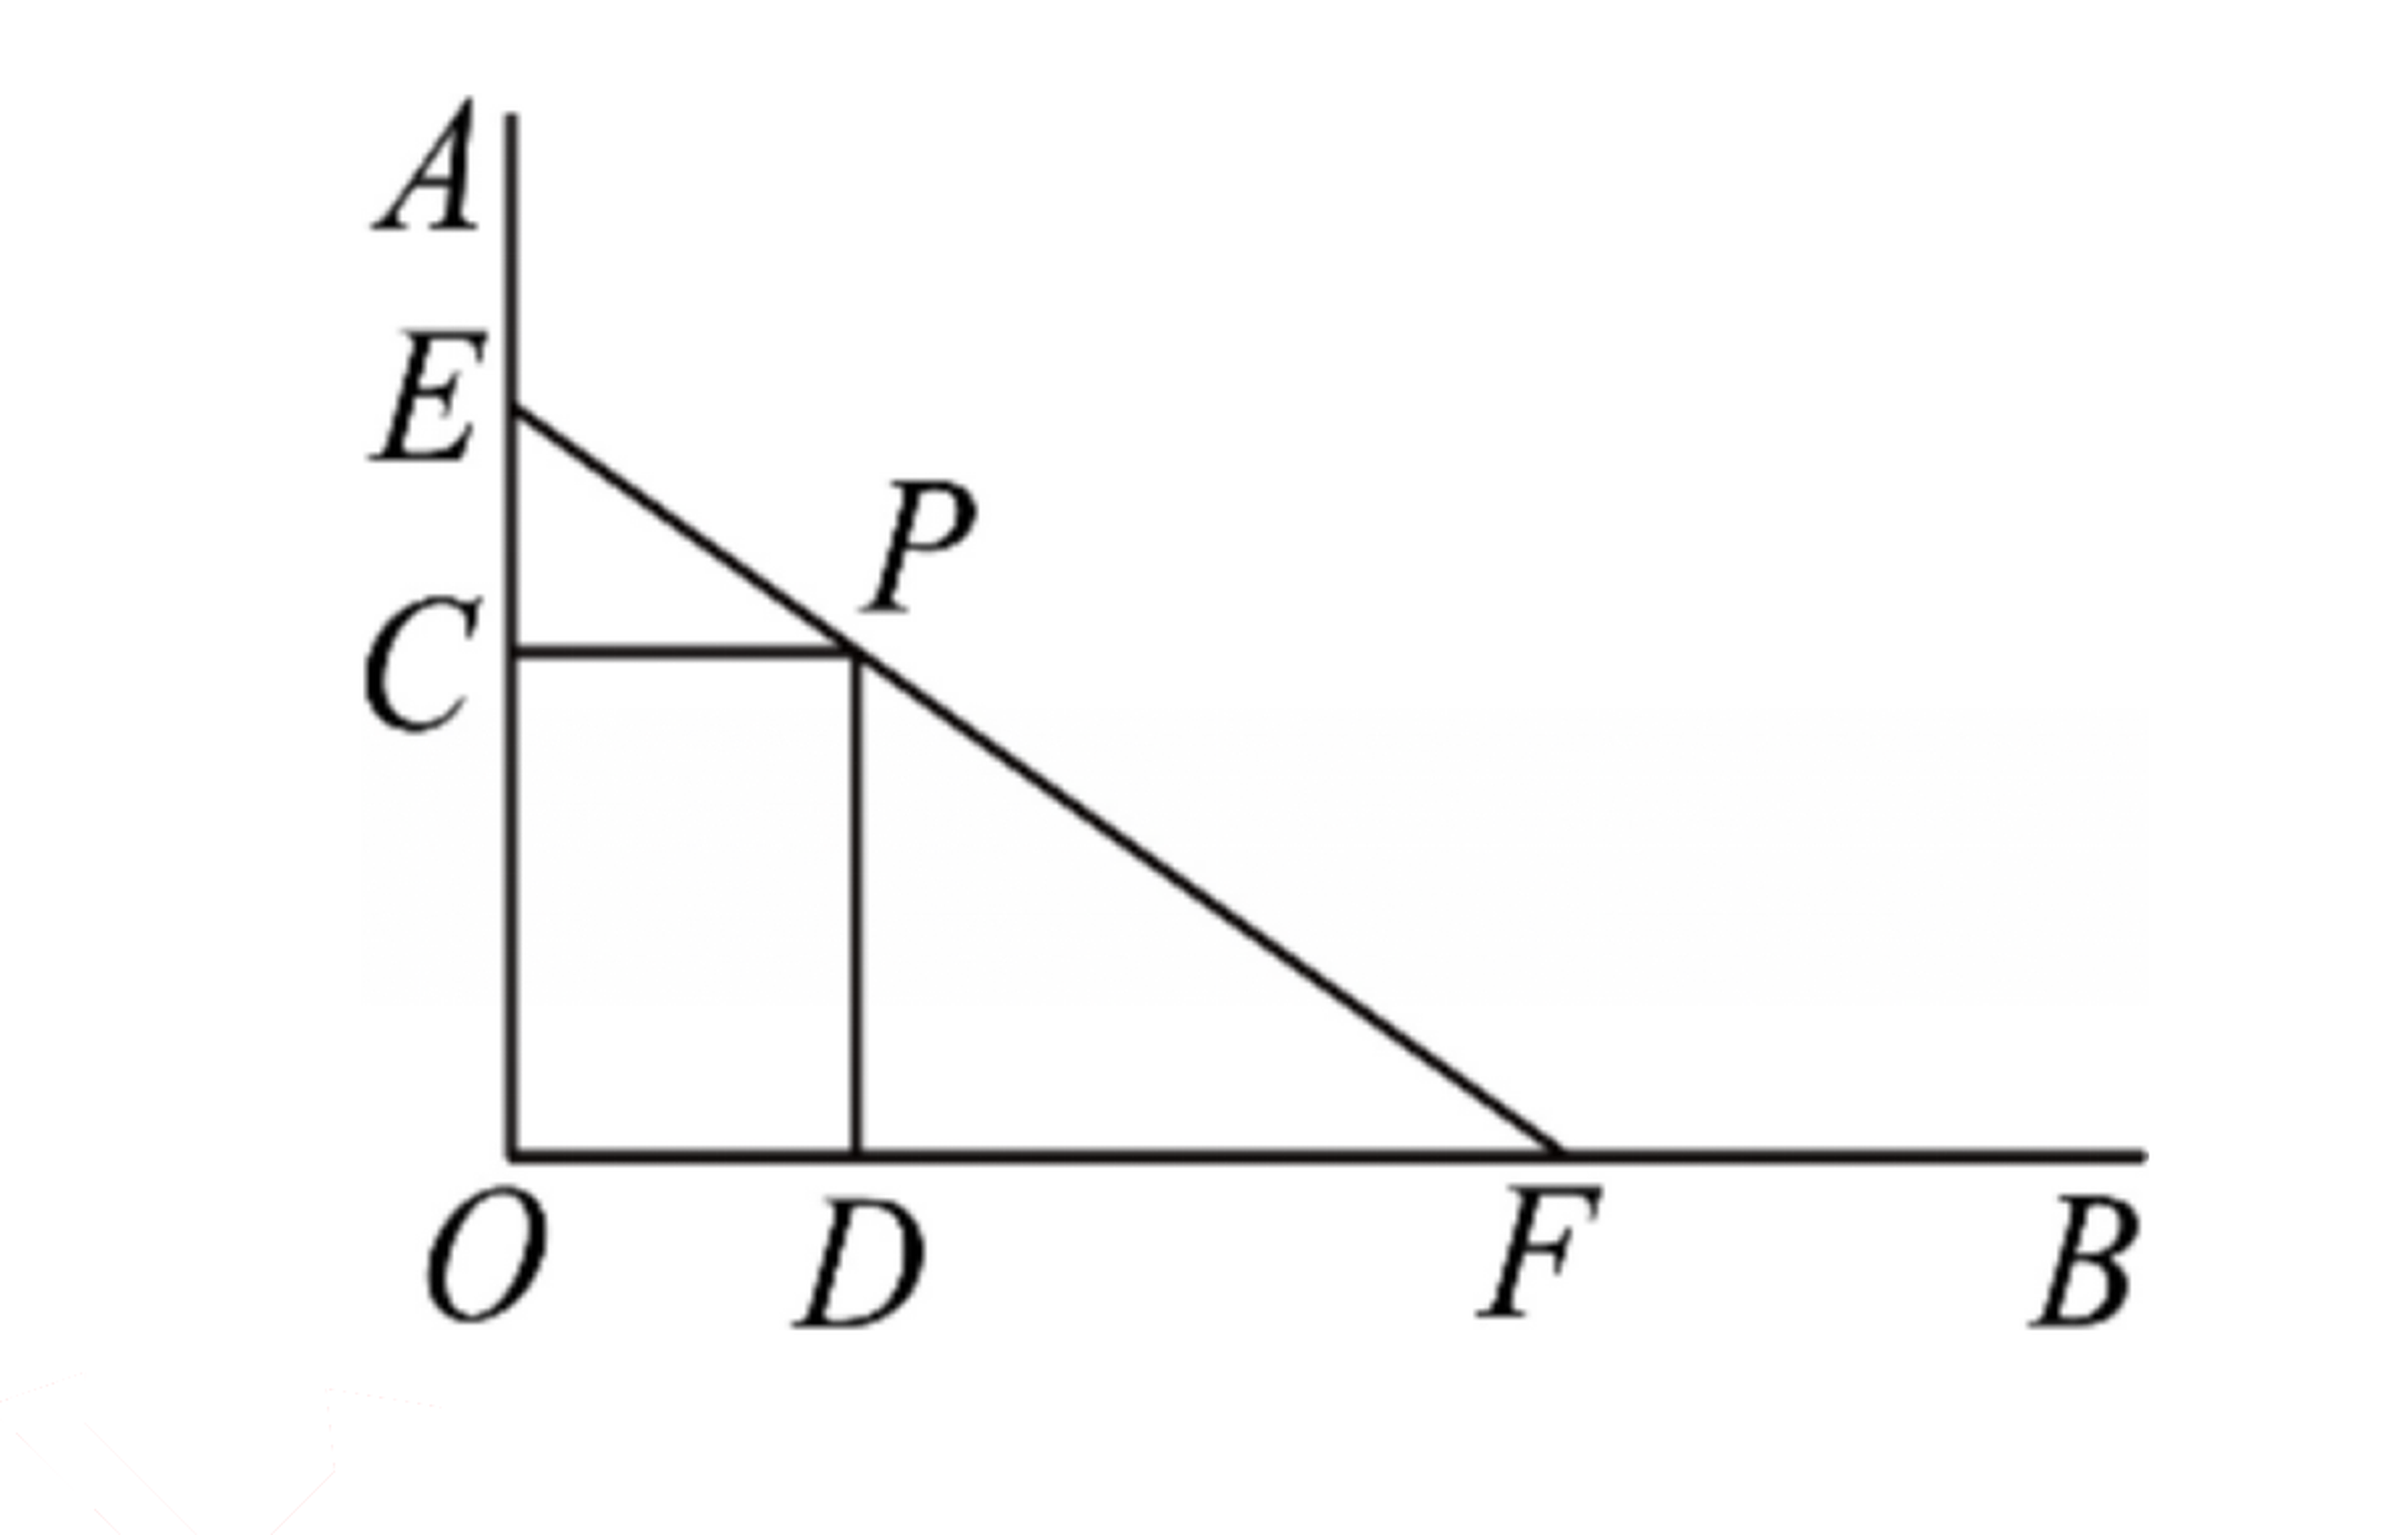
\includegraphics[width=0.32\textwidth]{figures/gao131_q19.png}
\end{center}

\ifanswer
\solbegin
\step{(1) 由题意得 $x\leq60$，}
\step{$\triangle PCE\sim\triangle FDP$，所以 $\dfrac{EC}{CP}=\dfrac{PD}{DF}$，即 $\dfrac{x}{25}=\dfrac{40}{DF}$，得 $DF=\dfrac{1000}{x}$m，}
\step{所以 $OF=OD+DF=\left(25+\dfrac{1000}{x}\right)$m，}
\step{所以 $25+\dfrac{1000}{x}\leq100$，解得 $x\geq\dfrac{40}{3}$；}
\step{综上，$\dfrac{40}{3}\leq x\leq60$；}
\step{(2) 由 $OE=OC+CE=(40+x)$m，}
\step{所以 $S=\dfrac12 OF\cdot OE=\dfrac12\left(25+\dfrac{1000}{x}\right)(40+x)$}
\step{$=\dfrac12\left(1000+25x+\dfrac{40000}{x}+1000\right)$m$^2$，}
\step{由基本不等式得 $S\geq\dfrac12\left(2000+2\sqrt{25x\cdot\dfrac{40000}{x}}\right)=2000$m$^2$，}
\step{当且仅当 $25x=\dfrac{40000}{x}$，即 $x=40$ 时取等号，}
\step{故 $EC=40$m 时，$S$ 取得最小值，为 $2000$m$^2$.}
\solend
\fi

\item 已知 $a\in\R$，函数 $y=ax^2+(3a+2)x+2a+3$.

(1) 当 $a=1$ 时，函数 $y=ax^2+(3a+2)x+2a+3$ 的图象与 $x$ 轴交于 $A(x_1,0)$，$B(x_2,0)$ 两点，求 $x_1^3+x_2^3$；

(2) 若关于 $x$ 的不等式 $ax^2+(3a+2)x+2a+3>2x$ 的解集为 $\R$，求实数 $a$ 的取值范围；

(3) 求关于 $x$ 的不等式 $y\geq1$ 的解集.

\ifanswer
\solbegin
\step{(1) 函数 $y=ax^2+(3a+2)x+2a+3$，当 $a=1$ 时，$y=x^2+5x+5$，}
\step{因为 $y=x^2+5x+5$ 的图象与 $x$ 轴交于 $A(x_1,0)$，$B(x_2,0)$ 两点，}
\step{即 $x^2+5x+5=0$ 的两个根为 $x_1$、$x_2$，}
\step{由根与系数的关系得 $x_1+x_2=-5$，$x_1x_2=5$，}
\step{所以 $x_1^2+x_2^2=(x_1+x_2)^2-2x_1x_2=25-10=15$，}
\step{所以 $x_1^3+x_2^3=(x_1+x_2)(x_1^2+x_2^2-x_1x_2)=-5\times(15-5)=-50$；}
\step{(2) 不等式 $ax^2+(3a+2)x+2a+3>2x$ 恒成立，得 $ax^2+3ax+2a+3>0$.}
\step{当 $a=0$ 时，$3>0$，恒成立，符合题意；}
\step{当 $a\neq0$ 时，若 $a<0$，二次函数 $ax^2+3ax+2a+3$ 开口向下，}
\step{一定存在小于零的部分，故不满足题意；}
\step{当 $a>0$ 时，若使 $ax^2+3ax+2a+3>0$ 恒成立，}
\step{只需 $\Delta=(3a)^2-4\times a\times(2a+3)=a^2-12a<0$，解得 $0<a<12$，}
\step{综上所述，$a$ 的取值范围为 $0\leq a<12$.}
\step{(3) 由 $y\geq1$，得 $ax^2+(3a+2)x+2a+3\geq1$，}
\step{即 $ax^2+(3a+2)x+2a+2\geq0$，即 $(ax+2a+2)(x+1)\geq0$，}
\step{当 $a=0$ 时，$2x+2\geq0$，解得 $x\geq-1$，}
\step{当 $a\neq0$ 时，}
\step{方程 $ax^2+(3a+2)x+2a+2=0$ 即为 $(x+1)(ax+2a+2)=0$，}
\step{解得 $x=-1$ 或 $x=-2-\dfrac2a$，令 $-1=-2-\dfrac2a$，即 $a=-2$，}
\step{当 $a>0$ 时，$-2-\dfrac2a<-1$，}
\step{不等式 $ax^2+(3a+2)x+2a+2\geq0$ 即为 $\left(x+\dfrac{2a+2}a\right)(x+1)\geq0$，}
\step{解得 $x\leq-2-\dfrac2a$ 或 $x\geq-1$；}
\step{当 $a<0$ 时，当 $-2-\dfrac2a<-1$，即 $a<-2$ 时，}
\step{不等式 $ax^2+(3a+2)x+2a+2\geq0$，即为 $\left(x+\dfrac{2a+2}a\right)(x+1)\leq0$，}
\step{解得 $-2-\dfrac2a\leq x\leq-1$；}
\step{当 $-2-\dfrac2a=-1$，即 $a=-2$，}
\step{不等式 $ax^2+(3a+2)x+2a+2\geq0$ 即为 $-2x^2-4x-2\geq0$，解得 $x=-1$，}
\step{当 $-2-\dfrac2a>-1$，即 $-2<a<0$ 时，}
\step{不等式 $ax^2+(3a+2)x+2a+2\geq0$ 即为 $\left(x+\dfrac{2a+2}a\right)(x+1)\leq0$，}
\step{解得 $-1\leq x\leq-2-\dfrac2a$，}
\step{综上所述，当 $a=0$ 时，解集为 $\{x\mid x\geq-1\}$；}
\step{当 $a>0$ 时，解集为 $\{x\mid x\leq-2-\dfrac2a$ 或 $x\geq-1\}$；}
\step{当 $a<-2$ 时，解集为 $\{x\mid -2-\dfrac2a\leq x\leq-1\}$；}
\step{当 $a=-2$ 时，解集为 $\{x\mid x=-1\}$；}
\step{当 $-2<a<0$ 时，解集为 $\{x\mid -1\leq x\leq-2-\dfrac2a\}$.}
\solend
\fi

\item 仔细阅读以下材料：【已知 $a$、$b\in(0,+\infty)$，$a+b=1$，求 $y=\dfrac1a+\dfrac2b$ 的最小值.

$y=\dfrac1a+\dfrac2b=\left(\dfrac1a+\dfrac2b\right)(a+b)=\dfrac ba+\dfrac{2a}b+3\geq3+2\sqrt2$，当且仅当 $\dfrac ba=\dfrac{2a}b$，即 $a=\sqrt2-1$，$b=2-\sqrt2$ 时取得等号，则 $y=\dfrac1a+\dfrac2b$ 的最小值为 $3+2\sqrt2$.

另 $y=\dfrac1a+\dfrac2b=\dfrac{a+b}a+\dfrac{2(a+b)}b=\dfrac ba+\dfrac{2a}b+3\geq3+2\sqrt2$，当且仅当 $\dfrac ba=\dfrac{2a}b$，即 $a=\sqrt2-1$，$b=2-\sqrt2$ 时取得等号，则 $y=\dfrac1a+\dfrac2b$ 的最小值为 $3+2\sqrt2$.】参考上述解法，求解下列问题.

(1) 若正实数 $x$、$y$ 满足 $x+y=1$，求 $\dfrac2x+\dfrac3y$ 的最小值；

(2) 已知 $x\in\left(0,\dfrac12\right)$，求 $t=\dfrac1x+\dfrac8{1-2x}$ 的最小值，并写出此时 $x$ 的值；

(3) 已知 $a$、$b\in(0,+\infty)$，$a+2b=1$，求 $p=\dfrac1{3a+4b}+\dfrac1{a+3b}$ 的最小值.

\ifanswer
\solbegin
\step{(1) 因为 $x>0,y>0$，且 $x+y=1$，}
\step{所以 $\dfrac2x+\dfrac3y=\left(\dfrac2x+\dfrac3y\right)(x+y)=2+\dfrac{2y}x+\dfrac{3x}y+3=5+\dfrac{2y}x+\dfrac{3x}y$，}
\step{由基本不等式得 $\dfrac{2y}x+\dfrac{3x}y\geq2\sqrt{\dfrac{2y}x\cdot\dfrac{3x}y}=2\sqrt6$，}
\step{当且仅当 $\dfrac{2y}x=\dfrac{3x}y$，即 $2y^2=3x^2$ 时，等号成立，}
\step{又因为 $x>0,y>0$ 且 $x+y=1$，此时 $x=\sqrt6-2,y=3-\sqrt6$，}
\step{所以 $\dfrac2x+\dfrac3y\geq5+2\sqrt6$，故 $\dfrac2x+\dfrac3y$ 的最小值为 $5+2\sqrt6$.}
\step{(2) 由 $0<x<\dfrac12$，则 $t=\dfrac1x+\dfrac8{1-2x}=\dfrac{2(1-2x+2x)}{2x}+\dfrac{8(1-2x+2x)}{1-2x}$}
\step{$=10+\dfrac{2\cdot(1-2x)}{2x}+\dfrac{8\cdot2x}{1-2x}\geq10+2\sqrt{\dfrac{2\cdot(1-2x)}{2x}\cdot\dfrac{8\cdot2x}{1-2x}}=18$，}
\step{当且仅当 $\dfrac{2\cdot(1-2x)}{2x}=\dfrac{8\cdot2x}{1-2x}$，即 $x=\dfrac16$ 时等号成立；}
\step{(3) 由 $a$、$b>0$，$a+2b=1$，则 $a=1-2b>0$，即 $0<b<\dfrac12$，}
\step{所以 $p=\dfrac1{3a+4b}+\dfrac1{a+3b}=\dfrac1{3a+6b-2b}+\dfrac1{a+2b+b}=\dfrac1{3-2b}+\dfrac1{1+b}$}
\step{$=\dfrac1{3-2b}+\dfrac2{2+2b}$，显然 $3-2b$、$2+2b>0$，}
\step{所以 $p=\dfrac15\cdot(3-2b+2+2b)\cdot\left(\dfrac1{3-2b}+\dfrac2{2+2b}\right)=\dfrac15\left[3+\dfrac{2+2b}{3-2b}+\dfrac{2(3-2b)}{2+2b}\right]$}
\step{$\geq\dfrac15\left[3+2\sqrt{\dfrac{2+2b}{3-2b}\cdot\dfrac{2(3-2b)}{2+2b}}\right]=\dfrac{3+2\sqrt2}5$，}
\step{当且仅当 $\dfrac{2+2b}{3-2b}=\dfrac{2(3-2b)}{2+2b}$，}
\step{即 $b=\dfrac{8-5\sqrt2}2$，$a=5\sqrt2-7$ 时等号成立.}
\solend
\fi

\end{enumerate}

\end{document}
"
%
% 原始材料：微信公众号"魔都数学加油站"文章，作者破晓，2026-11-13 18:18 发布；
% 连载"27学年高一131"，原文标题"27学年高一131——2026-2027年上海市六十中学高一上期中"；
% 原文链接：https://mp.weixin.qq.com/s/Nrbp3Uvt-sOGnOp4MEHemA。
% 正文为 11 张 PNG 页（01—05、09—11 为 2560x3620，06—08 为 4762x6735），
% 题目下印有【解析】或【答案】，为讲评版。题目、解析均据原图转录；
% 卷面粉红色水印"魔都数学加油站"及公众号页脚未录入。全卷仅第 19 题有 1 幅插图
% （矩形 OCPD 与小路 EF 的示意图），取 07.png 截图去水印。
%
% 卷首标题：原卷印作"2026-2027 年六十中学高一上期中"（公众号标题中的"上海市"
% 卷面标题行没有，本稿照卷面），年份区间按全稿惯例排 en dash；原卷未印副标题，
% 本卷为期中卷、跨集合与常用逻辑用语／不等式／函数三章，按题目内容标为
% "集合与常用逻辑用语、不等式、函数"（与 125／126／128／129 同期中卷口径相同）：
% 集合与逻辑见 Q3、Q4、Q7、Q13、Q17，不等式见 Q8、Q10、Q12、Q14、Q15、Q16、Q19、
% Q20、Q21，函数（指数／对数／幂函数、基本不等式应用）见 Q5、Q6、Q9、Q11、Q18、Q21。
%
% 题号体例：本卷共 19 题——一、填空题 3—12（10 题）、二、选择题 13—16（4 题）、
% 三、解答题 17—21（5 题）。三节分别 \setcounter{enumi}{2}／{12}／{16}。
%
% 与原卷的排版差异：
%   ① 原文从第 3 题起，本稿保留原题号（见上"题号体例"）；
%   ② 原卷每题下直接印【解析】／【答案】，本稿按全稿惯例置于答案版；第 3、4 题只印
%      【答案】，另提 \ans{}；第 13—16 题答案在解析末句"故选 …"，题干括号内留空、
%      不另提 \ans{}；其余各题印【解析】、无独立答案段；
%   ③ 原卷未印副标题，本稿按"知识模块"口径补出；
%   ④ 原卷填空横线按全稿惯例排为 \blankline[4.4em]；选择题括号排 \mbox{（\quad）}、
%      选项段前按惯例加 \keepwithprev；解答题不留作答区（原卷为讲评版，与 109—129 同）；
%   ⑤ 原卷数集排斜体 $R$／$N$，按全稿惯例改 \R／\N；绝对值排 \lvert…\rvert，
%      集合描述竖线排 \mid；不等号按全稿惯例排 \leqslant／\geqslant；
%   ⑥ 子题标号 (1)(2)(3) 原卷用半角括号，照录；圈数字 ①② 照录；
%   ⑦ 原卷第 19 题插图浮排在第 07 页题干右侧，本稿按体例就近置于题干"如图"之后
%      （居中 \includegraphics），图取原卷 07 页截图去水印；题前按惯例加
%      \needvspace{7cm} 守卫（照 高一120／127／129 成例），保证"题干 + 图"整块不被页边界切开；
%   ⑧ 原卷 Q9 题干跨 01—02 页、Q15 解析跨 03—04 页、Q16 材料跨 04—05 页、
%      Q17 题干跨 05—06 页、Q20 解析跨 08—09 页、Q21 解析跨 09—11 页，
%      本稿按题合并连续排版；末页第 11 页为 Q21 (3) 解析的续尾，按实际印刷行单列。
%   ⑨ 第 16 题材料英文括注原卷印作 (Cauchy – SchwarzInequality)（长横、Schwarz 与
%      Inequality 斜体连排无空格），本稿按全稿英文专名惯例排 \emph{(Cauchy-Schwarz Inequality)}；
%      第 15 题解析 B、D 两行原卷各印一步含 \lg m 的换底繁分数（2026-11-13 回原图核对补回，
%      本稿初转曾顺手去重跳过该步）。
%
% 判别式字形：第 20 题 (2) 解析 $\Delta=(3a)^2-4\times a\times(2a+3)=a^2-12a<0$
%   原卷排三角形（等腰、高；回 08.png 放大核对），照录 \Delta；全卷判别式仅此一处
%   （\triangle 另作第 19 题「$\triangle PCE\sim\triangle FDP$」的几何三角形记号）。
%
% 子集符号：第 17 题 (2) 解析 $P\subseteq Q$ 印带下划线，照录 \subseteq；
%   全卷未出现单线 \subset。
%
% 原卷存疑照录：
%   第 11 题解析末两式作 $\dfrac{2+m+\frac1n}{2n+2}=\dfrac{2n+mn+1}{2n+2}$，而第三式
%     分母 $\log_3 9+\log_3 2+\log_3 2=2+\frac2n$，与前一分母 $2n+2$ 不等，照录；
%   第 16 题材料 ①"对于所有实数 $x$ 和 $y$，有 $(a^2+b^2)(c^2+d^2)\geq(ac+bd)^2$"
%     句首用 $x$、$y$ 而式中用 $a$、$b$、$c$、$d$，照录；
%   第 20 题题干 (2) 作"解集为 $\R$"、解析 (2) 作"恒成立"，措辞不同，照录；
%   第 21 题材料把同一道题用两种解法连印两遍（"另 $y=\frac1a+\frac2b=\dots$"），照录；
%   第 21 题 (3) 解析末句"即 $b=\frac{8-5\sqrt2}{2}$，$a=5\sqrt2-7$ 时等号成立"
%     未另写"故最小值为 $\frac{3+2\sqrt2}{5}$"，照录；
%   第 12 题解析"所以 $e^a+e^b>e^c, a+b>c$"、第 8 题解析"$a>0$，$b>0$"、
%     第 18 题 (2)"$4x^2-4x+1<x^2+4x+4$，解得 $-\frac13<x<3$"等处数学式内
%     半角逗号，照录；
%   第 15 题解析用 $\lg$ 记常用对数（$\lg m$、$\lg 3$、$\lg 5$、$\lg 15$），照录。
%
% 行数复核：逐题数 \step 条数，合计 119 条（Q3：0；Q4：0；Q5：1；Q6：1；Q7：2；
% Q8：2；Q9：1；Q10：1；Q11：2；Q12：6；Q13：2；Q14：3；Q15：14；Q16：10；
% Q17：4；Q18：8；Q19：11；Q20：35；Q21：16），与原卷印刷行逐题相等
% （cases 块作一个印刷行计）。第 3、4 题只印【答案】，提 \ans{}，不计入 \step 账；
% 四道选择题答案均在解析末句，括号内留空、不另提 \ans{}。
%
\documentclass[a4paper,11pt]{article}
\usepackage{common}

\begin{document}

\examtitlest[3]{2026--2027 年六十中学高一上期中}{集合与常用逻辑用语、不等式、函数}

\bigsec{一、填空题}

\begin{enumerate}
\setcounter{enumi}{2}

\item 已知集合 $A=(0,4),B=[2,5]$，则 $A\cup B=$\blankline[4.4em].

\ifanswer
\ans{$(0,5]$}
\fi

\item 陈述句“$x=2$ 或 $y=3$”的否定形式为\blankline[4.4em].

\ifanswer
\ans{$x\neq2$ 且 $y\neq3$}
\fi

\item 函数 $y=a^{x-2}+15(a>0$ 且 $a\neq1)$ 的图象恒过定点的坐标为\blankline[4.4em].

\ifanswer
\solbegin
\step{函数 $y=a^{x-2}+15$ 的图象恒过定点 $A(2,16)$.}
\solend
\fi

\item 用有理数指数幂的形式来化简：$\dfrac{\sqrt{a\cdot\sqrt[3]{a^4}}}{\left(a^{\frac13}\right)^2}=$\blankline[4.4em].

\ifanswer
\solbegin
\step{原式 $=\dfrac{\sqrt{a\cdot a^{\frac43}}}{a^{\frac23}}=\dfrac{\sqrt{a^{\frac73}}}{a^{\frac23}}=\dfrac{a^{\frac76}}{a^{\frac23}}=a^{\frac76-\frac23}=a^{\frac12}(a>0)$.}
\solend
\fi

\item 已知集合 $A=\left\{x\mid \dfrac6{6-x}\in\N\text{ 且 }x\in\N\right\}$，则用列举法表示集合 $A=$\blankline[4.4em].

\ifanswer
\solbegin
\step{当 $x=0$ 时，$\dfrac6{6-0}=1\in\N$，当 $x=3$ 时，$\dfrac6{6-3}=2\in\N$，}
\step{当 $x=4$ 时，$\dfrac6{6-4}=3\in\N$，当 $x=5$ 时，$\dfrac6{6-5}=6\in\N$，故 $A=\{0,3,4,5\}$.}
\solend
\fi

\item 已知 $a>0$，$b>0$，且 $ab=\dfrac12$，则 $\dfrac1a+\dfrac8b$ 的最小值是\blankline[4.4em].

\ifanswer
\solbegin
\step{$a>0$，$b>0$，且 $ab=\dfrac12$，则 $\dfrac1a+\dfrac8b\geq2\sqrt{\dfrac8{ab}}=8$，}
\step{当且仅当 $\dfrac1a=\dfrac8b$，即 $a=\dfrac14,b=2$ 时取等号，故最小值为 $8$.}
\solend
\fi

\item 心理学家有时用函数 $L(t)=A(1-e^{-kt})$ 测定在时间 $t$（单位：$min$）内能够记忆的量 $L$，其中 $A$ 表示需要记忆的量，$k$ 表示记忆率. 假设一个学生需要记忆的量为 $200$ 个单词，此时 $L$ 表示在时间 $t$ 内该生能够记忆的单词个数. 已知该生在 $5min$ 内能够记忆 $20$ 个单词，则 $k$ 的值约为\blankline[4.4em]（结果保留四位小数）.

\ifanswer
\solbegin
\step{由题意得 $200(1-e^{-5k})=20$，所以 $e^{-5k}=0.9$，解得 $k\approx0.0211$.}
\solend
\fi

\item 设 $x\in\R$，方程 $\lvert 3x-2\rvert+\lvert 1-x\rvert=\lvert 2x-1\rvert$ 的解集是\blankline[4.4em].

\ifanswer
\solbegin
\step{由三角不等式得 $(3x-2)(1-x)\geq0$，故解集是 $\left[\dfrac23,1\right]$.}
\solend
\fi

\item 已知 $3^m=5$，$n=\log_2 3$，则 $\log_{36}90$ 可用 $m$、$n$ 表示为\blankline[4.4em].

\ifanswer
\solbegin
\step{由 $3^m=5$，又 $n=\log_2 3$，得 $m=\log_3 5$，$\log_3 2=\dfrac{\log_2 2}{\log_2 3}=\dfrac1n$，}
\step{所以 $\log_{36}90=\dfrac{\log_3 90}{\log_3 36}=\dfrac{\log_3 9+\log_3 2+\log_3 5}{\log_3 9+\log_3 2+\log_3 2}=\dfrac{2+m+\frac1n}{2n+2}=\dfrac{2n+mn+1}{2n+2}$.}
\solend
\fi

\item 若定义域为 $I=(0,m]$ 的函数 $f(x)=e^x$ 满足：对任意能构成三角形三边长的实数 $a$、$b$、$c\in I$，均有 $f(a)$、$f(b)$、$f(c)$ 也能构成三角形三边长，则 $m$ 的最大值为\blankline[4.4em].

\ifanswer
\solbegin
\step{$f(x)=e^x$ 在 $I=(0,m]$ 上严格增，所以 $f(x)\in(1,e^m]$，不妨设 $0<a\leq b\leq c$，}
\step{因为对任意能构成三角形三边长的实数 $a,b,c\in I$，均有 $f(a)$，$f(b)$，$f(c)$}
\step{也能构成三角形三边长，所以 $e^a+e^b>e^c, a+b>c$，}
\step{因为 $e^a+e^b\geq2\sqrt{e^ae^b}=2\sqrt{e^{a+b}}>e^c$，所以 $4e^{a+b}>e^{2c}$，}
\step{因为对任意 $a,b,c\in I$ 都成立，所以 $4e^c\geq e^{2c}$，所以 $e^c\leq4$，所以 $c\leq\ln4$，}
\step{所以 $m\leq\ln4$，所以 $m$ 的最大值为 $\ln4$.}
\solend
\fi

\end{enumerate}

\bigsec{二、选择题}

\begin{enumerate}
\setcounter{enumi}{12}

\item 已知 $m,n$ 是非零自然数，命题 $\alpha:mn$ 是奇数，命题 $\beta:m$ 或 $n$ 是奇数，则 $\alpha$ 是 $\beta$ 的\mbox{（\quad）}

\keepwithprev
A. 充分非必要条件\qquad\qquad B. 必要非充分条件

C. 充要条件\qquad\qquad D. 既非充分又非必要条件

\ifanswer
\solbegin
\step{$mn$ 是奇数 $\Leftrightarrow$ $m$、$n$ 都是奇数，所以 $\alpha$ 能推出 $\beta$，充分性成立，}
\step{但 $\beta$ 推不出 $\alpha$，必要性不成立，所以 $\alpha$ 是 $\beta$ 的充分非必要条件. 故选 $A$.}
\solend
\fi

\item 关于 $x$ 的不等式 $x^2-mx+n+5\leq0$ 的解集是 $[1,8]$，那么 $\log_m n=$\mbox{（\quad）}

\keepwithprev
A. $\dfrac13$\qquad\qquad B. $-3$\qquad\qquad C. $-2$\qquad\qquad D. $\dfrac12$

\ifanswer
\solbegin
\step{由题意得 $x^2-mx+n+5=0$ 的解为 $1$，$8$，}
\step{由根与系数的关系得 $\begin{cases}1+8=m\\1\times8=n+5\end{cases}$，解得 $m=9$，$n=3$，}
\step{所以 $\log_m n=\log_9 3=\dfrac12\log_3 3=\dfrac12$. 故选 $D$.}
\solend
\fi

\item 已知正实数 $x$、$y$、$z$ 满足 $3^x=5^y=15^z$，则下列说法中不正确的是\mbox{（\quad）}

\keepwithprev
A. $\dfrac1x+\dfrac1y=\dfrac1z$\qquad\qquad B. $x+y>2z$\qquad\qquad C. $3x>5y>15z$\qquad\qquad D. $x\cdot y>4z^2$

\ifanswer
\solbegin
\step{已知正实数 $x$、$y$、$z$，则设 $3^x=5^y=15^z=m>1$，}
\step{所以 $x=\log_3 m$，$y=\log_5 m$，$z=\log_{15} m$，}
\step{对于 $A$，$\dfrac1x+\dfrac1y=\dfrac1{\log_3 m}+\dfrac1{\log_5 m}=\log_m 3+\log_m 5=\log_m 15=\dfrac1z$，故 $A$ 正确；}
\step{对于 $B$，因为 $\dfrac{x+y}{z}=\dfrac{x}{z}+\dfrac{y}{z}=\dfrac{\log_3 m}{\log_{15} m}+\dfrac{\log_5 m}{\log_{15} m}=\dfrac{\dfrac{\lg m}{\lg3}}{\dfrac{\lg m}{\lg15}}+\dfrac{\dfrac{\lg m}{\lg5}}{\dfrac{\lg m}{\lg15}}=\dfrac{\lg15}{\lg3}+\dfrac{\lg15}{\lg5}$，}
\step{$=\dfrac{\lg3+\lg5}{\lg3}+\dfrac{\lg3+\lg5}{\lg5}=2+\dfrac{\lg5}{\lg3}+\dfrac{\lg3}{\lg5}=2+\log_3 5+\log_5 3$，}
\step{又 $\log_3 5>0$，$\log_5 3>0$，所以 $2+\log_3 5+\log_5 3>2$，}
\step{所以 $\dfrac{x+y}{z}>2$，即 $x+y>2z$，故 $B$ 正确；}
\step{对于 $C$，因为 $\dfrac5x=5\log_m 3=\log_m 243$，$\dfrac3y=3\log_m 5=\log_m 125$，}
\step{所以 $\dfrac5x>\dfrac3y$，即 $3x<5y$，故 $C$ 错误；}
\step{对于 $D$，$\dfrac{xy}{z^2}=\dfrac{x}{z}\cdot\dfrac{y}{z}=\dfrac{\log_3 m}{\log_{15} m}\cdot\dfrac{\log_5 m}{\log_{15} m}=\dfrac{\dfrac{\lg m}{\lg3}}{\dfrac{\lg m}{\lg15}}\cdot\dfrac{\dfrac{\lg m}{\lg5}}{\dfrac{\lg m}{\lg15}}=\dfrac{\lg15}{\lg3}\cdot\dfrac{\lg15}{\lg5}$}
\step{$=\dfrac{\lg3+\lg5}{\lg3}\cdot\dfrac{\lg3+\lg5}{\lg5}=\left(1+\dfrac{\lg5}{\lg3}\right)\left(1+\dfrac{\lg3}{\lg5}\right)=2+\dfrac{\lg5}{\lg3}+\dfrac{\lg3}{\lg5}$}
\step{$\geq2+2\sqrt{\dfrac{\lg5}{\lg3}\cdot\dfrac{\lg3}{\lg5}}=2+2=4$，又 $\lg3\neq\lg5$，故等号不成立，}
\step{所以 $\dfrac{xy}{z^2}>4$，即 $xy>4z^2$，故 $D$ 正确.}
\step{故选 $C$.}
\solend
\fi

\item 柯西不等式 \emph{(Cauchy-Schwarz Inequality)} 是一种在数学和物理学中广泛使用的不等式，它是由法国数学家奥古斯丁$\cdot$路易$\cdot$柯西提出的，柯西不等式可以用于证明其他不等式，也可以用于解决一些数学问题. 以下是柯西不等式的原始形式：

①对于所有实数 $x$ 和 $y$，有 $(a^2+b^2)(c^2+d^2)\geq(ac+bd)^2$.

②等式条件：当且仅当 $ad-bc=0$ 时，等号成立.

例：已知 $x+2y=2$，由柯西不等式 $(x^2+y^2)(1^2+2^2)\geq(x+2y)^2$，可得 $(x^2+y^2)_{min}=\dfrac45$.

现给出以下两个命题：

①若 $a^2+b^2=1$，则 $2a+3b$ 的最大值为 $\sqrt{13}$；

②若 $1<a<3$，则 $\sqrt{a-1}+\sqrt{6-2a}$ 的最大值为 $\sqrt6$；

则运用柯西不等式，判断以下正确的选项有\mbox{（\quad）}

\keepwithprev
A. ①为真命题；②为真命题\qquad\qquad B. ①为真命题；②为假命题

C. ①为假命题；②为真命题\qquad\qquad D. ①为假命题；②为假命题

\ifanswer
\solbegin
\step{由柯西不等式得 $(a^2+b^2)(2^2+3^2)\geq(2a+3b)^2$.}
\step{因为 $a^2+b^2=1$，所以 $(2^2+3^2)\geq(2a+3b)^2$，即 $13\geq(2a+3b)^2$，}
\step{所以 $-\sqrt{13}\leq2a+3b\leq\sqrt{13}$，则 $(2a+3b)_{max}=\sqrt{13}$，}
\step{当且仅当 $3a=2b$ 时取等号，故①正确.}
\step{令 $x=\sqrt{a-1}$，$y=\sqrt{3-a}$，则 $x^2+y^2=a-1+3-a=2$，}
\step{由柯西不等式得 $(\sqrt{a-1}+\sqrt{6-2a})^2=(\sqrt{a-1}+\sqrt2\cdot\sqrt{3-a})^2=(x+\sqrt2 y)^2$}
\step{$\leq[1^2+(\sqrt2)^2](x^2+y^2)$，}
\step{因为 $x^2+y^2=2$，所以 $(\sqrt{a-1}+\sqrt{6-2a})^2\leq6$，}
\step{当且仅当 $\sqrt{3-a}=\sqrt2\sqrt{a-1}$ 取等号，所以 $\sqrt{a-1}+\sqrt{6-2a}\leq\sqrt6$，故②正确.}
\step{故选 $A$.}
\solend
\fi

\end{enumerate}

\bigsec{三、解答题}

\begin{enumerate}
\setcounter{enumi}{16}

\item 已知集合 $P=\left\{x\mid \dfrac{3x-1}{x+2}<1\right\}$，集合 $Q=\{x\mid\lvert x-a\rvert\leq2\}$.

(1) 求集合 $P$；

(2) 若“$x\in P$”是“$x\in Q$”的充分非必要条件，求实数 $a$ 的取值范围.

\ifanswer
\solbegin
\step{(1) 集合 $P=\left\{x\mid \dfrac{3x-1}{x+2}<1\right\}$，得 $\dfrac{2x-3}{x+2}<0$，解得 $P=\left(-2,\dfrac32\right)$.}
\step{(2) 集合 $Q=\{x\mid\lvert x-a\rvert\leq2\}=\{x\mid a-2\leq x\leq2+a\}$，}
\step{由“$x\in P$”是“$x\in Q$”的充分非必要条件，得 $P\subseteq Q$，}
\step{得 $\begin{cases}-2\geq a-2\\\dfrac32\leq2+a\\a-2<2+a\end{cases}$，解得 $a\in\left[-\dfrac12,0\right]$.}
\solend
\fi

\item 已知幂函数 $f(x)=(m^2-4m+4)\cdot x^{2m-4}$ 在 $(-\infty,0)$ 上是严格减函数.

(1) 求函数 $y=f(x)$ 的解析式；

(2) 若 $f(1-2x)<f(x+2)$，求 $x$ 的取值范围.

\ifanswer
\solbegin
\step{(1) 由幂函数的定义得 $m^2-4m+4=1$，解得 $m=1$ 或 $3$，}
\step{当 $m=1$ 时，$f(x)=x^{-2}=\dfrac1{x^2}$，在 $(-\infty,0)$ 上严格增，不符合题意，}
\step{当 $m=3$ 时，$f(x)=x^2$，在 $(-\infty,0)$ 上严格减，符合题意，}
\step{所以 $f(x)=x^2$；}
\step{(2) 由函数 $f(x)=x^2$ 图象关于 $y$ 轴对称，且在 $[0,+\infty)$ 上严格增，}
\step{则 $f(1-2x)<f(x+2)$ 可化为 $\lvert1-2x\rvert<\lvert x+2\rvert$，}
\step{平方得 $4x^2-4x+1<x^2+4x+4$，解得 $-\dfrac13<x<3$，}
\step{所以 $x$ 的取值范围是 $\left(-\dfrac13,3\right)$.}
\solend
\fi

% 第 19 题是"题干 + 图"约 7cm 的一整块，守卫放在 \item 之前（放 \item 之后会失效）
\needvspace{7cm}
\item 如图，$OA$、$OB$ 是两条长度足够长的互相垂直的笔直小路，矩形 $OCPD$ 的顶点 $C$，$D$ 分别在 $OA$、$OB$ 上，且该矩形区域内种满了荷花. 为了让观赏者有更好的观赏体验，现计划经过点 $P$ 修一条小路 $EF$，其中点 $E$ 在小路 $OA$ 上，点 $F$ 在小路 $OB$ 上，并在 $\triangle OEF$ 区域内种满荷花. 已知 $OD=25m$，$OC=40m$，且小路 $EF$ 要完全位于一个以 $O$ 为顶点的，边长为 $100$ m 的正方形内部（包括边界）. 记 $\triangle OEF$ 的面积为 $S$m$^2$.

(1) 设 $EC=x\cdot m$，试用 $x$ 表示 $OF$，并求 $x$ 的取值范围.

(2) 当 $EC$ 的长度为多少时，$S$ 取得最小值？最小值是多少？

\begin{center}
% 图取原卷 07.png 截图去粉色水印，2.8× LANCZOS 放大
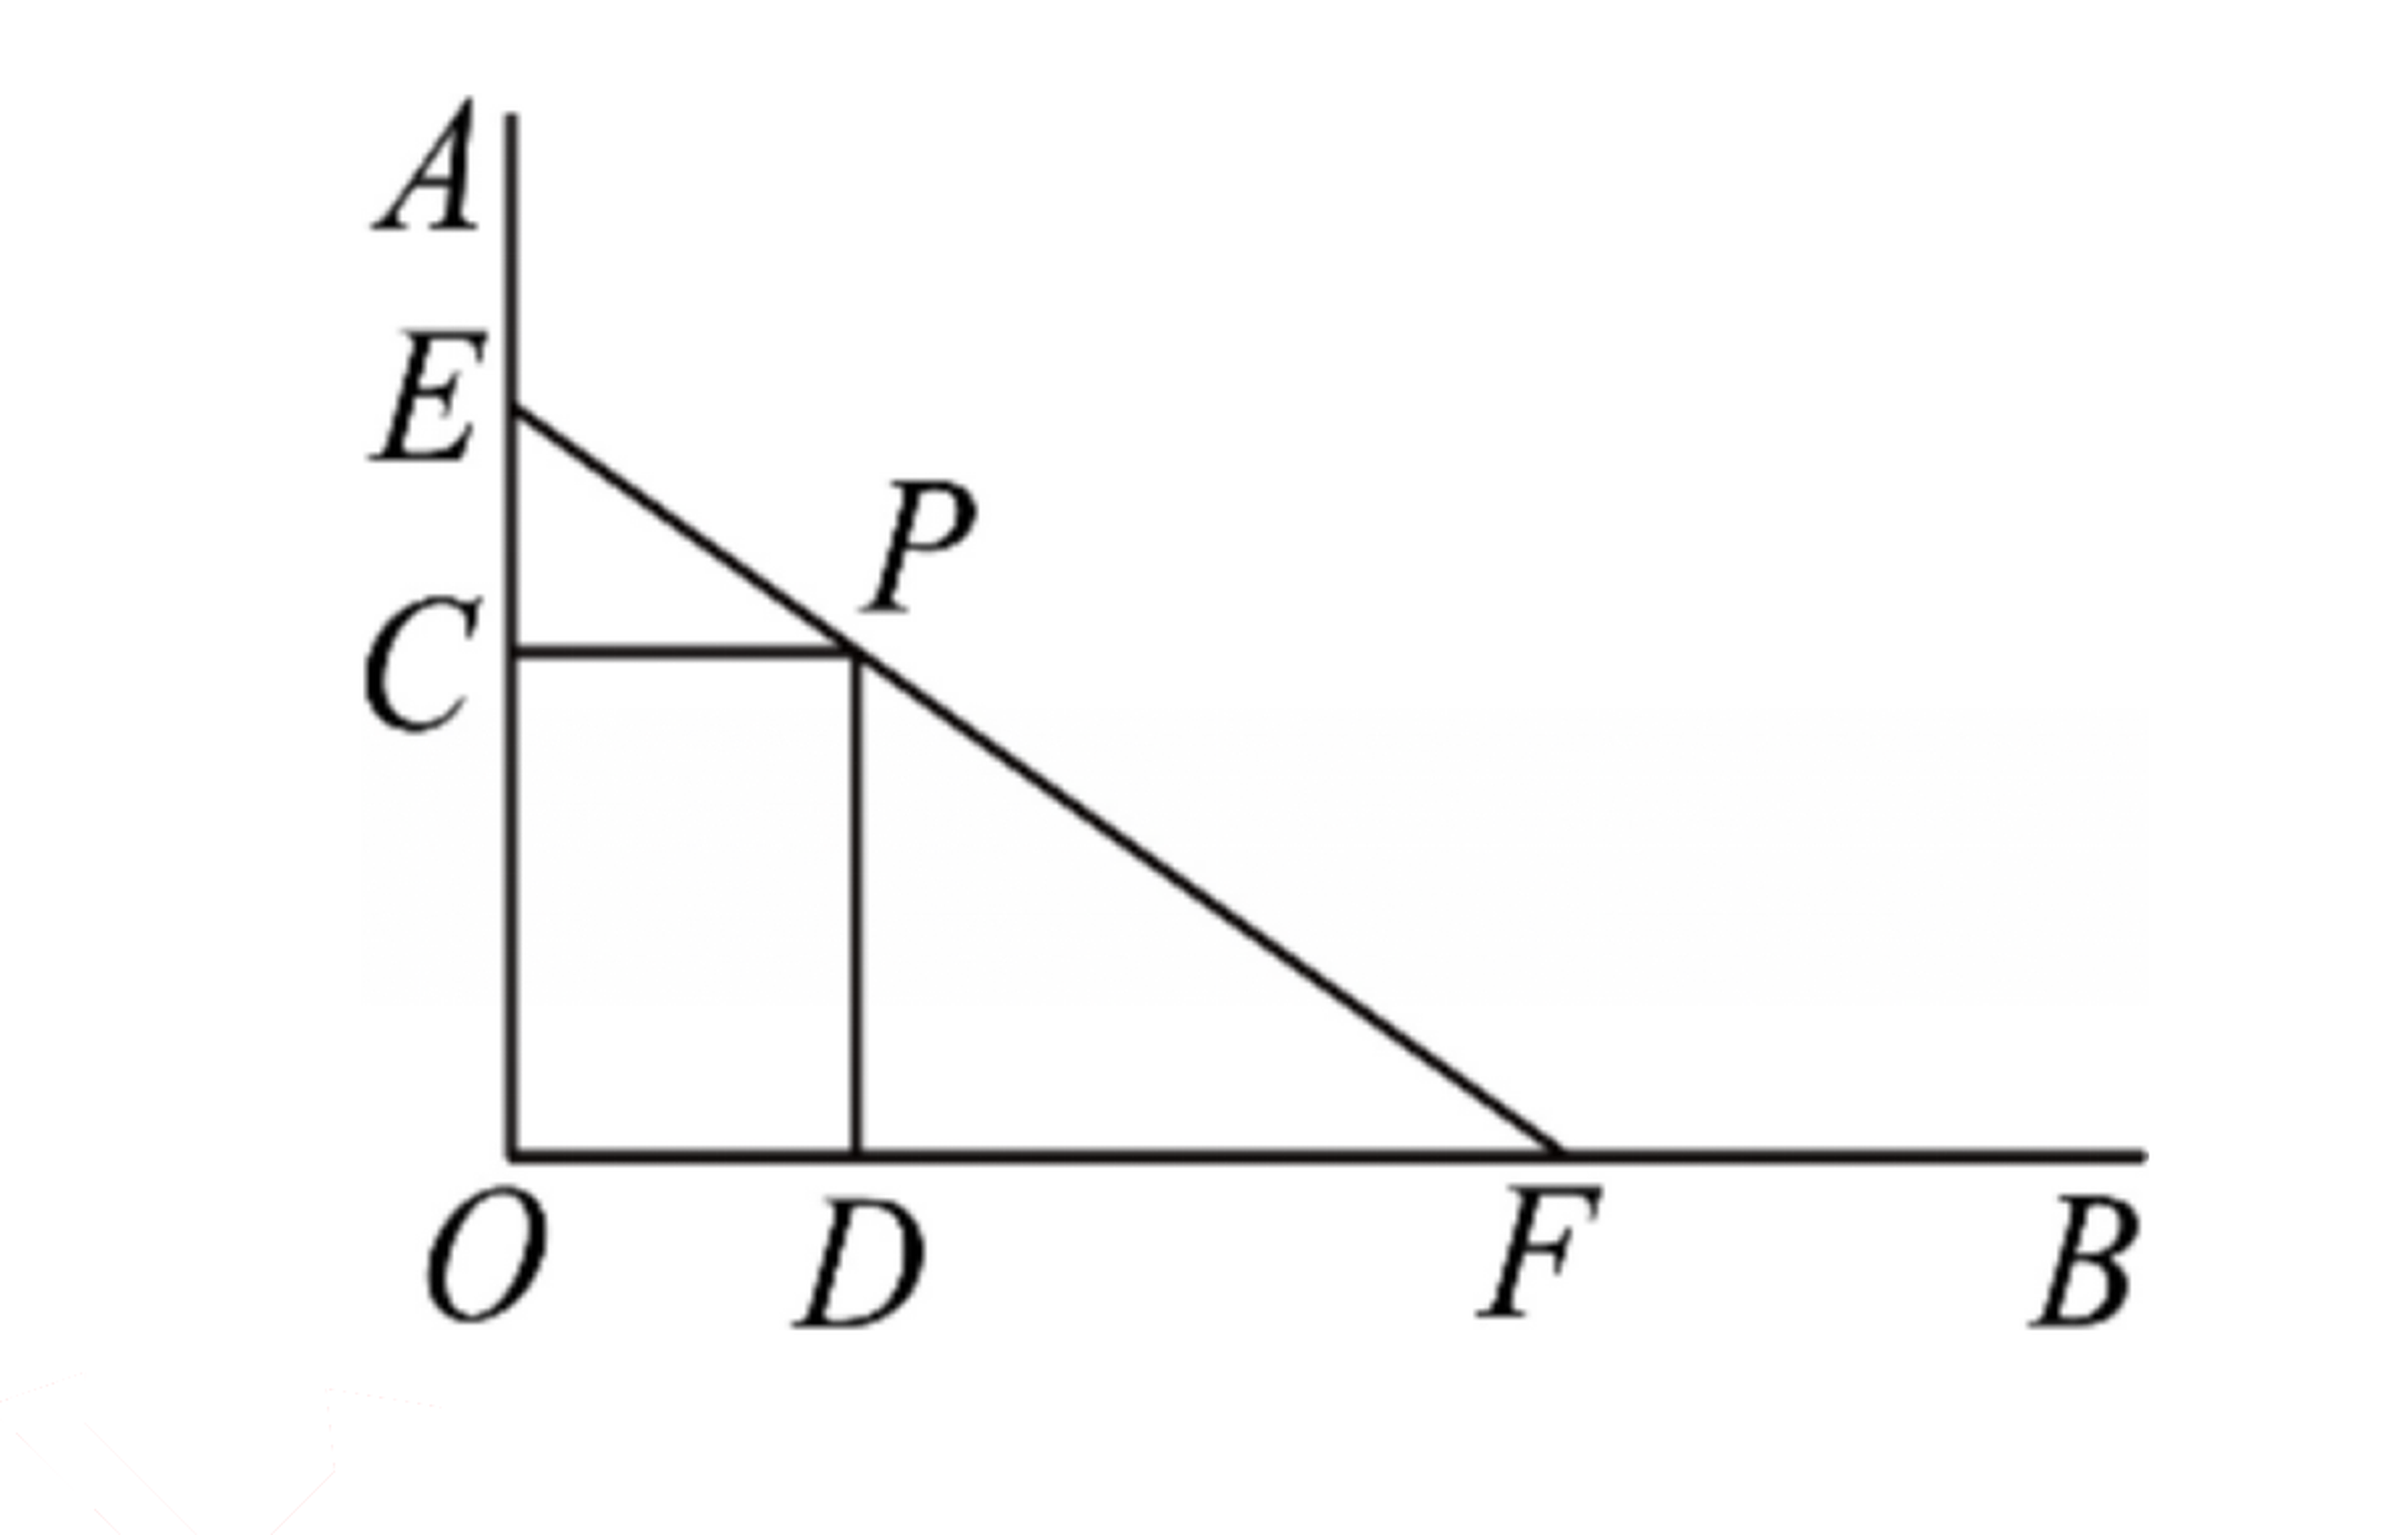
\includegraphics[width=0.32\textwidth]{figures/gao131_q19.png}
\end{center}

\ifanswer
\solbegin
\step{(1) 由题意得 $x\leq60$，}
\step{$\triangle PCE\sim\triangle FDP$，所以 $\dfrac{EC}{CP}=\dfrac{PD}{DF}$，即 $\dfrac{x}{25}=\dfrac{40}{DF}$，得 $DF=\dfrac{1000}{x}$m，}
\step{所以 $OF=OD+DF=\left(25+\dfrac{1000}{x}\right)$m，}
\step{所以 $25+\dfrac{1000}{x}\leq100$，解得 $x\geq\dfrac{40}{3}$；}
\step{综上，$\dfrac{40}{3}\leq x\leq60$；}
\step{(2) 由 $OE=OC+CE=(40+x)$m，}
\step{所以 $S=\dfrac12 OF\cdot OE=\dfrac12\left(25+\dfrac{1000}{x}\right)(40+x)$}
\step{$=\dfrac12\left(1000+25x+\dfrac{40000}{x}+1000\right)$m$^2$，}
\step{由基本不等式得 $S\geq\dfrac12\left(2000+2\sqrt{25x\cdot\dfrac{40000}{x}}\right)=2000$m$^2$，}
\step{当且仅当 $25x=\dfrac{40000}{x}$，即 $x=40$ 时取等号，}
\step{故 $EC=40$m 时，$S$ 取得最小值，为 $2000$m$^2$.}
\solend
\fi

\item 已知 $a\in\R$，函数 $y=ax^2+(3a+2)x+2a+3$.

(1) 当 $a=1$ 时，函数 $y=ax^2+(3a+2)x+2a+3$ 的图象与 $x$ 轴交于 $A(x_1,0)$，$B(x_2,0)$ 两点，求 $x_1^3+x_2^3$；

(2) 若关于 $x$ 的不等式 $ax^2+(3a+2)x+2a+3>2x$ 的解集为 $\R$，求实数 $a$ 的取值范围；

(3) 求关于 $x$ 的不等式 $y\geq1$ 的解集.

\ifanswer
\solbegin
\step{(1) 函数 $y=ax^2+(3a+2)x+2a+3$，当 $a=1$ 时，$y=x^2+5x+5$，}
\step{因为 $y=x^2+5x+5$ 的图象与 $x$ 轴交于 $A(x_1,0)$，$B(x_2,0)$ 两点，}
\step{即 $x^2+5x+5=0$ 的两个根为 $x_1$、$x_2$，}
\step{由根与系数的关系得 $x_1+x_2=-5$，$x_1x_2=5$，}
\step{所以 $x_1^2+x_2^2=(x_1+x_2)^2-2x_1x_2=25-10=15$，}
\step{所以 $x_1^3+x_2^3=(x_1+x_2)(x_1^2+x_2^2-x_1x_2)=-5\times(15-5)=-50$；}
\step{(2) 不等式 $ax^2+(3a+2)x+2a+3>2x$ 恒成立，得 $ax^2+3ax+2a+3>0$.}
\step{当 $a=0$ 时，$3>0$，恒成立，符合题意；}
\step{当 $a\neq0$ 时，若 $a<0$，二次函数 $ax^2+3ax+2a+3$ 开口向下，}
\step{一定存在小于零的部分，故不满足题意；}
\step{当 $a>0$ 时，若使 $ax^2+3ax+2a+3>0$ 恒成立，}
\step{只需 $\Delta=(3a)^2-4\times a\times(2a+3)=a^2-12a<0$，解得 $0<a<12$，}
\step{综上所述，$a$ 的取值范围为 $0\leq a<12$.}
\step{(3) 由 $y\geq1$，得 $ax^2+(3a+2)x+2a+3\geq1$，}
\step{即 $ax^2+(3a+2)x+2a+2\geq0$，即 $(ax+2a+2)(x+1)\geq0$，}
\step{当 $a=0$ 时，$2x+2\geq0$，解得 $x\geq-1$，}
\step{当 $a\neq0$ 时，}
\step{方程 $ax^2+(3a+2)x+2a+2=0$ 即为 $(x+1)(ax+2a+2)=0$，}
\step{解得 $x=-1$ 或 $x=-2-\dfrac2a$，令 $-1=-2-\dfrac2a$，即 $a=-2$，}
\step{当 $a>0$ 时，$-2-\dfrac2a<-1$，}
\step{不等式 $ax^2+(3a+2)x+2a+2\geq0$ 即为 $\left(x+\dfrac{2a+2}a\right)(x+1)\geq0$，}
\step{解得 $x\leq-2-\dfrac2a$ 或 $x\geq-1$；}
\step{当 $a<0$ 时，当 $-2-\dfrac2a<-1$，即 $a<-2$ 时，}
\step{不等式 $ax^2+(3a+2)x+2a+2\geq0$，即为 $\left(x+\dfrac{2a+2}a\right)(x+1)\leq0$，}
\step{解得 $-2-\dfrac2a\leq x\leq-1$；}
\step{当 $-2-\dfrac2a=-1$，即 $a=-2$，}
\step{不等式 $ax^2+(3a+2)x+2a+2\geq0$ 即为 $-2x^2-4x-2\geq0$，解得 $x=-1$，}
\step{当 $-2-\dfrac2a>-1$，即 $-2<a<0$ 时，}
\step{不等式 $ax^2+(3a+2)x+2a+2\geq0$ 即为 $\left(x+\dfrac{2a+2}a\right)(x+1)\leq0$，}
\step{解得 $-1\leq x\leq-2-\dfrac2a$，}
\step{综上所述，当 $a=0$ 时，解集为 $\{x\mid x\geq-1\}$；}
\step{当 $a>0$ 时，解集为 $\{x\mid x\leq-2-\dfrac2a$ 或 $x\geq-1\}$；}
\step{当 $a<-2$ 时，解集为 $\{x\mid -2-\dfrac2a\leq x\leq-1\}$；}
\step{当 $a=-2$ 时，解集为 $\{x\mid x=-1\}$；}
\step{当 $-2<a<0$ 时，解集为 $\{x\mid -1\leq x\leq-2-\dfrac2a\}$.}
\solend
\fi

\item 仔细阅读以下材料：【已知 $a$、$b\in(0,+\infty)$，$a+b=1$，求 $y=\dfrac1a+\dfrac2b$ 的最小值.

$y=\dfrac1a+\dfrac2b=\left(\dfrac1a+\dfrac2b\right)(a+b)=\dfrac ba+\dfrac{2a}b+3\geq3+2\sqrt2$，当且仅当 $\dfrac ba=\dfrac{2a}b$，即 $a=\sqrt2-1$，$b=2-\sqrt2$ 时取得等号，则 $y=\dfrac1a+\dfrac2b$ 的最小值为 $3+2\sqrt2$.

另 $y=\dfrac1a+\dfrac2b=\dfrac{a+b}a+\dfrac{2(a+b)}b=\dfrac ba+\dfrac{2a}b+3\geq3+2\sqrt2$，当且仅当 $\dfrac ba=\dfrac{2a}b$，即 $a=\sqrt2-1$，$b=2-\sqrt2$ 时取得等号，则 $y=\dfrac1a+\dfrac2b$ 的最小值为 $3+2\sqrt2$.】参考上述解法，求解下列问题.

(1) 若正实数 $x$、$y$ 满足 $x+y=1$，求 $\dfrac2x+\dfrac3y$ 的最小值；

(2) 已知 $x\in\left(0,\dfrac12\right)$，求 $t=\dfrac1x+\dfrac8{1-2x}$ 的最小值，并写出此时 $x$ 的值；

(3) 已知 $a$、$b\in(0,+\infty)$，$a+2b=1$，求 $p=\dfrac1{3a+4b}+\dfrac1{a+3b}$ 的最小值.

\ifanswer
\solbegin
\step{(1) 因为 $x>0,y>0$，且 $x+y=1$，}
\step{所以 $\dfrac2x+\dfrac3y=\left(\dfrac2x+\dfrac3y\right)(x+y)=2+\dfrac{2y}x+\dfrac{3x}y+3=5+\dfrac{2y}x+\dfrac{3x}y$，}
\step{由基本不等式得 $\dfrac{2y}x+\dfrac{3x}y\geq2\sqrt{\dfrac{2y}x\cdot\dfrac{3x}y}=2\sqrt6$，}
\step{当且仅当 $\dfrac{2y}x=\dfrac{3x}y$，即 $2y^2=3x^2$ 时，等号成立，}
\step{又因为 $x>0,y>0$ 且 $x+y=1$，此时 $x=\sqrt6-2,y=3-\sqrt6$，}
\step{所以 $\dfrac2x+\dfrac3y\geq5+2\sqrt6$，故 $\dfrac2x+\dfrac3y$ 的最小值为 $5+2\sqrt6$.}
\step{(2) 由 $0<x<\dfrac12$，则 $t=\dfrac1x+\dfrac8{1-2x}=\dfrac{2(1-2x+2x)}{2x}+\dfrac{8(1-2x+2x)}{1-2x}$}
\step{$=10+\dfrac{2\cdot(1-2x)}{2x}+\dfrac{8\cdot2x}{1-2x}\geq10+2\sqrt{\dfrac{2\cdot(1-2x)}{2x}\cdot\dfrac{8\cdot2x}{1-2x}}=18$，}
\step{当且仅当 $\dfrac{2\cdot(1-2x)}{2x}=\dfrac{8\cdot2x}{1-2x}$，即 $x=\dfrac16$ 时等号成立；}
\step{(3) 由 $a$、$b>0$，$a+2b=1$，则 $a=1-2b>0$，即 $0<b<\dfrac12$，}
\step{所以 $p=\dfrac1{3a+4b}+\dfrac1{a+3b}=\dfrac1{3a+6b-2b}+\dfrac1{a+2b+b}=\dfrac1{3-2b}+\dfrac1{1+b}$}
\step{$=\dfrac1{3-2b}+\dfrac2{2+2b}$，显然 $3-2b$、$2+2b>0$，}
\step{所以 $p=\dfrac15\cdot(3-2b+2+2b)\cdot\left(\dfrac1{3-2b}+\dfrac2{2+2b}\right)=\dfrac15\left[3+\dfrac{2+2b}{3-2b}+\dfrac{2(3-2b)}{2+2b}\right]$}
\step{$\geq\dfrac15\left[3+2\sqrt{\dfrac{2+2b}{3-2b}\cdot\dfrac{2(3-2b)}{2+2b}}\right]=\dfrac{3+2\sqrt2}5$，}
\step{当且仅当 $\dfrac{2+2b}{3-2b}=\dfrac{2(3-2b)}{2+2b}$，}
\step{即 $b=\dfrac{8-5\sqrt2}2$，$a=5\sqrt2-7$ 时等号成立.}
\solend
\fi

\end{enumerate}

\end{document}
"
%
% 原始材料：微信公众号"魔都数学加油站"文章，作者破晓，2026-11-13 18:18 发布；
% 连载"27学年高一131"，原文标题"27学年高一131——2026-2027年上海市六十中学高一上期中"；
% 原文链接：https://mp.weixin.qq.com/s/Nrbp3Uvt-sOGnOp4MEHemA。
% 正文为 11 张 PNG 页（01—05、09—11 为 2560x3620，06—08 为 4762x6735），
% 题目下印有【解析】或【答案】，为讲评版。题目、解析均据原图转录；
% 卷面粉红色水印"魔都数学加油站"及公众号页脚未录入。全卷仅第 19 题有 1 幅插图
% （矩形 OCPD 与小路 EF 的示意图），取 07.png 截图去水印。
%
% 卷首标题：原卷印作"2026-2027 年六十中学高一上期中"（公众号标题中的"上海市"
% 卷面标题行没有，本稿照卷面），年份区间按全稿惯例排 en dash；原卷未印副标题，
% 本卷为期中卷、跨集合与常用逻辑用语／不等式／函数三章，按题目内容标为
% "集合与常用逻辑用语、不等式、函数"（与 125／126／128／129 同期中卷口径相同）：
% 集合与逻辑见 Q3、Q4、Q7、Q13、Q17，不等式见 Q8、Q10、Q12、Q14、Q15、Q16、Q19、
% Q20、Q21，函数（指数／对数／幂函数、基本不等式应用）见 Q5、Q6、Q9、Q11、Q18、Q21。
%
% 题号体例：本卷共 19 题——一、填空题 3—12（10 题）、二、选择题 13—16（4 题）、
% 三、解答题 17—21（5 题）。三节分别 \setcounter{enumi}{2}／{12}／{16}。
%
% 与原卷的排版差异：
%   ① 原文从第 3 题起，本稿保留原题号（见上"题号体例"）；
%   ② 原卷每题下直接印【解析】／【答案】，本稿按全稿惯例置于答案版；第 3、4 题只印
%      【答案】，另提 \ans{}；第 13—16 题答案在解析末句"故选 …"，题干括号内留空、
%      不另提 \ans{}；其余各题印【解析】、无独立答案段；
%   ③ 原卷未印副标题，本稿按"知识模块"口径补出；
%   ④ 原卷填空横线按全稿惯例排为 \blankline[4.4em]；选择题括号排 \mbox{（\quad）}、
%      选项段前按惯例加 \keepwithprev；解答题不留作答区（原卷为讲评版，与 109—129 同）；
%   ⑤ 原卷数集排斜体 $R$／$N$，按全稿惯例改 \R／\N；绝对值排 \lvert…\rvert，
%      集合描述竖线排 \mid；不等号按全稿惯例排 \leqslant／\geqslant；
%   ⑥ 子题标号 (1)(2)(3) 原卷用半角括号，照录；圈数字 ①② 照录；
%   ⑦ 原卷第 19 题插图浮排在第 07 页题干右侧，本稿按体例就近置于题干"如图"之后
%      （居中 \includegraphics），图取原卷 07 页截图去水印；题前按惯例加
%      \needvspace{7cm} 守卫（照 高一120／127／129 成例），保证"题干 + 图"整块不被页边界切开；
%   ⑧ 原卷 Q9 题干跨 01—02 页、Q15 解析跨 03—04 页、Q16 材料跨 04—05 页、
%      Q17 题干跨 05—06 页、Q20 解析跨 08—09 页、Q21 解析跨 09—11 页，
%      本稿按题合并连续排版；末页第 11 页为 Q21 (3) 解析的续尾，按实际印刷行单列。
%   ⑨ 第 16 题材料英文括注原卷印作 (Cauchy – SchwarzInequality)（长横、Schwarz 与
%      Inequality 斜体连排无空格），本稿按全稿英文专名惯例排 \emph{(Cauchy-Schwarz Inequality)}；
%      第 15 题解析 B、D 两行原卷各印一步含 \lg m 的换底繁分数（2026-11-13 回原图核对补回，
%      本稿初转曾顺手去重跳过该步）。
%
% 判别式字形：第 20 题 (2) 解析 $\Delta=(3a)^2-4\times a\times(2a+3)=a^2-12a<0$
%   原卷排三角形（等腰、高；回 08.png 放大核对），照录 \Delta；全卷判别式仅此一处
%   （\triangle 另作第 19 题「$\triangle PCE\sim\triangle FDP$」的几何三角形记号）。
%
% 子集符号：第 17 题 (2) 解析 $P\subseteq Q$ 印带下划线，照录 \subseteq；
%   全卷未出现单线 \subset。
%
% 原卷存疑照录：
%   第 11 题解析末两式作 $\dfrac{2+m+\frac1n}{2n+2}=\dfrac{2n+mn+1}{2n+2}$，而第三式
%     分母 $\log_3 9+\log_3 2+\log_3 2=2+\frac2n$，与前一分母 $2n+2$ 不等，照录；
%   第 16 题材料 ①"对于所有实数 $x$ 和 $y$，有 $(a^2+b^2)(c^2+d^2)\geq(ac+bd)^2$"
%     句首用 $x$、$y$ 而式中用 $a$、$b$、$c$、$d$，照录；
%   第 20 题题干 (2) 作"解集为 $\R$"、解析 (2) 作"恒成立"，措辞不同，照录；
%   第 21 题材料把同一道题用两种解法连印两遍（"另 $y=\frac1a+\frac2b=\dots$"），照录；
%   第 21 题 (3) 解析末句"即 $b=\frac{8-5\sqrt2}{2}$，$a=5\sqrt2-7$ 时等号成立"
%     未另写"故最小值为 $\frac{3+2\sqrt2}{5}$"，照录；
%   第 12 题解析"所以 $e^a+e^b>e^c, a+b>c$"、第 8 题解析"$a>0$，$b>0$"、
%     第 18 题 (2)"$4x^2-4x+1<x^2+4x+4$，解得 $-\frac13<x<3$"等处数学式内
%     半角逗号，照录；
%   第 15 题解析用 $\lg$ 记常用对数（$\lg m$、$\lg 3$、$\lg 5$、$\lg 15$），照录。
%
% 行数复核：逐题数 \step 条数，合计 119 条（Q3：0；Q4：0；Q5：1；Q6：1；Q7：2；
% Q8：2；Q9：1；Q10：1；Q11：2；Q12：6；Q13：2；Q14：3；Q15：14；Q16：10；
% Q17：4；Q18：8；Q19：11；Q20：35；Q21：16），与原卷印刷行逐题相等
% （cases 块作一个印刷行计）。第 3、4 题只印【答案】，提 \ans{}，不计入 \step 账；
% 四道选择题答案均在解析末句，括号内留空、不另提 \ans{}。
%
\documentclass[a4paper,11pt]{article}
\usepackage{common}

\begin{document}

\examtitlest[3]{2026--2027 年六十中学高一上期中}{集合与常用逻辑用语、不等式、函数}

\bigsec{一、填空题}

\begin{enumerate}
\setcounter{enumi}{2}

\item 已知集合 $A=(0,4),B=[2,5]$，则 $A\cup B=$\blankline[4.4em].

\ifanswer
\ans{$(0,5]$}
\fi

\item 陈述句“$x=2$ 或 $y=3$”的否定形式为\blankline[4.4em].

\ifanswer
\ans{$x\neq2$ 且 $y\neq3$}
\fi

\item 函数 $y=a^{x-2}+15(a>0$ 且 $a\neq1)$ 的图象恒过定点的坐标为\blankline[4.4em].

\ifanswer
\solbegin
\step{函数 $y=a^{x-2}+15$ 的图象恒过定点 $A(2,16)$.}
\solend
\fi

\item 用有理数指数幂的形式来化简：$\dfrac{\sqrt{a\cdot\sqrt[3]{a^4}}}{\left(a^{\frac13}\right)^2}=$\blankline[4.4em].

\ifanswer
\solbegin
\step{原式 $=\dfrac{\sqrt{a\cdot a^{\frac43}}}{a^{\frac23}}=\dfrac{\sqrt{a^{\frac73}}}{a^{\frac23}}=\dfrac{a^{\frac76}}{a^{\frac23}}=a^{\frac76-\frac23}=a^{\frac12}(a>0)$.}
\solend
\fi

\item 已知集合 $A=\left\{x\mid \dfrac6{6-x}\in\N\text{ 且 }x\in\N\right\}$，则用列举法表示集合 $A=$\blankline[4.4em].

\ifanswer
\solbegin
\step{当 $x=0$ 时，$\dfrac6{6-0}=1\in\N$，当 $x=3$ 时，$\dfrac6{6-3}=2\in\N$，}
\step{当 $x=4$ 时，$\dfrac6{6-4}=3\in\N$，当 $x=5$ 时，$\dfrac6{6-5}=6\in\N$，故 $A=\{0,3,4,5\}$.}
\solend
\fi

\item 已知 $a>0$，$b>0$，且 $ab=\dfrac12$，则 $\dfrac1a+\dfrac8b$ 的最小值是\blankline[4.4em].

\ifanswer
\solbegin
\step{$a>0$，$b>0$，且 $ab=\dfrac12$，则 $\dfrac1a+\dfrac8b\geq2\sqrt{\dfrac8{ab}}=8$，}
\step{当且仅当 $\dfrac1a=\dfrac8b$，即 $a=\dfrac14,b=2$ 时取等号，故最小值为 $8$.}
\solend
\fi

\item 心理学家有时用函数 $L(t)=A(1-e^{-kt})$ 测定在时间 $t$（单位：$min$）内能够记忆的量 $L$，其中 $A$ 表示需要记忆的量，$k$ 表示记忆率. 假设一个学生需要记忆的量为 $200$ 个单词，此时 $L$ 表示在时间 $t$ 内该生能够记忆的单词个数. 已知该生在 $5min$ 内能够记忆 $20$ 个单词，则 $k$ 的值约为\blankline[4.4em]（结果保留四位小数）.

\ifanswer
\solbegin
\step{由题意得 $200(1-e^{-5k})=20$，所以 $e^{-5k}=0.9$，解得 $k\approx0.0211$.}
\solend
\fi

\item 设 $x\in\R$，方程 $\lvert 3x-2\rvert+\lvert 1-x\rvert=\lvert 2x-1\rvert$ 的解集是\blankline[4.4em].

\ifanswer
\solbegin
\step{由三角不等式得 $(3x-2)(1-x)\geq0$，故解集是 $\left[\dfrac23,1\right]$.}
\solend
\fi

\item 已知 $3^m=5$，$n=\log_2 3$，则 $\log_{36}90$ 可用 $m$、$n$ 表示为\blankline[4.4em].

\ifanswer
\solbegin
\step{由 $3^m=5$，又 $n=\log_2 3$，得 $m=\log_3 5$，$\log_3 2=\dfrac{\log_2 2}{\log_2 3}=\dfrac1n$，}
\step{所以 $\log_{36}90=\dfrac{\log_3 90}{\log_3 36}=\dfrac{\log_3 9+\log_3 2+\log_3 5}{\log_3 9+\log_3 2+\log_3 2}=\dfrac{2+m+\frac1n}{2n+2}=\dfrac{2n+mn+1}{2n+2}$.}
\solend
\fi

\item 若定义域为 $I=(0,m]$ 的函数 $f(x)=e^x$ 满足：对任意能构成三角形三边长的实数 $a$、$b$、$c\in I$，均有 $f(a)$、$f(b)$、$f(c)$ 也能构成三角形三边长，则 $m$ 的最大值为\blankline[4.4em].

\ifanswer
\solbegin
\step{$f(x)=e^x$ 在 $I=(0,m]$ 上严格增，所以 $f(x)\in(1,e^m]$，不妨设 $0<a\leq b\leq c$，}
\step{因为对任意能构成三角形三边长的实数 $a,b,c\in I$，均有 $f(a)$，$f(b)$，$f(c)$}
\step{也能构成三角形三边长，所以 $e^a+e^b>e^c, a+b>c$，}
\step{因为 $e^a+e^b\geq2\sqrt{e^ae^b}=2\sqrt{e^{a+b}}>e^c$，所以 $4e^{a+b}>e^{2c}$，}
\step{因为对任意 $a,b,c\in I$ 都成立，所以 $4e^c\geq e^{2c}$，所以 $e^c\leq4$，所以 $c\leq\ln4$，}
\step{所以 $m\leq\ln4$，所以 $m$ 的最大值为 $\ln4$.}
\solend
\fi

\end{enumerate}

\bigsec{二、选择题}

\begin{enumerate}
\setcounter{enumi}{12}

\item 已知 $m,n$ 是非零自然数，命题 $\alpha:mn$ 是奇数，命题 $\beta:m$ 或 $n$ 是奇数，则 $\alpha$ 是 $\beta$ 的\mbox{（\quad）}

\keepwithprev
A. 充分非必要条件\qquad\qquad B. 必要非充分条件

C. 充要条件\qquad\qquad D. 既非充分又非必要条件

\ifanswer
\solbegin
\step{$mn$ 是奇数 $\Leftrightarrow$ $m$、$n$ 都是奇数，所以 $\alpha$ 能推出 $\beta$，充分性成立，}
\step{但 $\beta$ 推不出 $\alpha$，必要性不成立，所以 $\alpha$ 是 $\beta$ 的充分非必要条件. 故选 $A$.}
\solend
\fi

\item 关于 $x$ 的不等式 $x^2-mx+n+5\leq0$ 的解集是 $[1,8]$，那么 $\log_m n=$\mbox{（\quad）}

\keepwithprev
A. $\dfrac13$\qquad\qquad B. $-3$\qquad\qquad C. $-2$\qquad\qquad D. $\dfrac12$

\ifanswer
\solbegin
\step{由题意得 $x^2-mx+n+5=0$ 的解为 $1$，$8$，}
\step{由根与系数的关系得 $\begin{cases}1+8=m\\1\times8=n+5\end{cases}$，解得 $m=9$，$n=3$，}
\step{所以 $\log_m n=\log_9 3=\dfrac12\log_3 3=\dfrac12$. 故选 $D$.}
\solend
\fi

\item 已知正实数 $x$、$y$、$z$ 满足 $3^x=5^y=15^z$，则下列说法中不正确的是\mbox{（\quad）}

\keepwithprev
A. $\dfrac1x+\dfrac1y=\dfrac1z$\qquad\qquad B. $x+y>2z$\qquad\qquad C. $3x>5y>15z$\qquad\qquad D. $x\cdot y>4z^2$

\ifanswer
\solbegin
\step{已知正实数 $x$、$y$、$z$，则设 $3^x=5^y=15^z=m>1$，}
\step{所以 $x=\log_3 m$，$y=\log_5 m$，$z=\log_{15} m$，}
\step{对于 $A$，$\dfrac1x+\dfrac1y=\dfrac1{\log_3 m}+\dfrac1{\log_5 m}=\log_m 3+\log_m 5=\log_m 15=\dfrac1z$，故 $A$ 正确；}
\step{对于 $B$，因为 $\dfrac{x+y}{z}=\dfrac{x}{z}+\dfrac{y}{z}=\dfrac{\log_3 m}{\log_{15} m}+\dfrac{\log_5 m}{\log_{15} m}=\dfrac{\dfrac{\lg m}{\lg3}}{\dfrac{\lg m}{\lg15}}+\dfrac{\dfrac{\lg m}{\lg5}}{\dfrac{\lg m}{\lg15}}=\dfrac{\lg15}{\lg3}+\dfrac{\lg15}{\lg5}$，}
\step{$=\dfrac{\lg3+\lg5}{\lg3}+\dfrac{\lg3+\lg5}{\lg5}=2+\dfrac{\lg5}{\lg3}+\dfrac{\lg3}{\lg5}=2+\log_3 5+\log_5 3$，}
\step{又 $\log_3 5>0$，$\log_5 3>0$，所以 $2+\log_3 5+\log_5 3>2$，}
\step{所以 $\dfrac{x+y}{z}>2$，即 $x+y>2z$，故 $B$ 正确；}
\step{对于 $C$，因为 $\dfrac5x=5\log_m 3=\log_m 243$，$\dfrac3y=3\log_m 5=\log_m 125$，}
\step{所以 $\dfrac5x>\dfrac3y$，即 $3x<5y$，故 $C$ 错误；}
\step{对于 $D$，$\dfrac{xy}{z^2}=\dfrac{x}{z}\cdot\dfrac{y}{z}=\dfrac{\log_3 m}{\log_{15} m}\cdot\dfrac{\log_5 m}{\log_{15} m}=\dfrac{\dfrac{\lg m}{\lg3}}{\dfrac{\lg m}{\lg15}}\cdot\dfrac{\dfrac{\lg m}{\lg5}}{\dfrac{\lg m}{\lg15}}=\dfrac{\lg15}{\lg3}\cdot\dfrac{\lg15}{\lg5}$}
\step{$=\dfrac{\lg3+\lg5}{\lg3}\cdot\dfrac{\lg3+\lg5}{\lg5}=\left(1+\dfrac{\lg5}{\lg3}\right)\left(1+\dfrac{\lg3}{\lg5}\right)=2+\dfrac{\lg5}{\lg3}+\dfrac{\lg3}{\lg5}$}
\step{$\geq2+2\sqrt{\dfrac{\lg5}{\lg3}\cdot\dfrac{\lg3}{\lg5}}=2+2=4$，又 $\lg3\neq\lg5$，故等号不成立，}
\step{所以 $\dfrac{xy}{z^2}>4$，即 $xy>4z^2$，故 $D$ 正确.}
\step{故选 $C$.}
\solend
\fi

\item 柯西不等式 \emph{(Cauchy-Schwarz Inequality)} 是一种在数学和物理学中广泛使用的不等式，它是由法国数学家奥古斯丁$\cdot$路易$\cdot$柯西提出的，柯西不等式可以用于证明其他不等式，也可以用于解决一些数学问题. 以下是柯西不等式的原始形式：

①对于所有实数 $x$ 和 $y$，有 $(a^2+b^2)(c^2+d^2)\geq(ac+bd)^2$.

②等式条件：当且仅当 $ad-bc=0$ 时，等号成立.

例：已知 $x+2y=2$，由柯西不等式 $(x^2+y^2)(1^2+2^2)\geq(x+2y)^2$，可得 $(x^2+y^2)_{min}=\dfrac45$.

现给出以下两个命题：

①若 $a^2+b^2=1$，则 $2a+3b$ 的最大值为 $\sqrt{13}$；

②若 $1<a<3$，则 $\sqrt{a-1}+\sqrt{6-2a}$ 的最大值为 $\sqrt6$；

则运用柯西不等式，判断以下正确的选项有\mbox{（\quad）}

\keepwithprev
A. ①为真命题；②为真命题\qquad\qquad B. ①为真命题；②为假命题

C. ①为假命题；②为真命题\qquad\qquad D. ①为假命题；②为假命题

\ifanswer
\solbegin
\step{由柯西不等式得 $(a^2+b^2)(2^2+3^2)\geq(2a+3b)^2$.}
\step{因为 $a^2+b^2=1$，所以 $(2^2+3^2)\geq(2a+3b)^2$，即 $13\geq(2a+3b)^2$，}
\step{所以 $-\sqrt{13}\leq2a+3b\leq\sqrt{13}$，则 $(2a+3b)_{max}=\sqrt{13}$，}
\step{当且仅当 $3a=2b$ 时取等号，故①正确.}
\step{令 $x=\sqrt{a-1}$，$y=\sqrt{3-a}$，则 $x^2+y^2=a-1+3-a=2$，}
\step{由柯西不等式得 $(\sqrt{a-1}+\sqrt{6-2a})^2=(\sqrt{a-1}+\sqrt2\cdot\sqrt{3-a})^2=(x+\sqrt2 y)^2$}
\step{$\leq[1^2+(\sqrt2)^2](x^2+y^2)$，}
\step{因为 $x^2+y^2=2$，所以 $(\sqrt{a-1}+\sqrt{6-2a})^2\leq6$，}
\step{当且仅当 $\sqrt{3-a}=\sqrt2\sqrt{a-1}$ 取等号，所以 $\sqrt{a-1}+\sqrt{6-2a}\leq\sqrt6$，故②正确.}
\step{故选 $A$.}
\solend
\fi

\end{enumerate}

\bigsec{三、解答题}

\begin{enumerate}
\setcounter{enumi}{16}

\item 已知集合 $P=\left\{x\mid \dfrac{3x-1}{x+2}<1\right\}$，集合 $Q=\{x\mid\lvert x-a\rvert\leq2\}$.

(1) 求集合 $P$；

(2) 若“$x\in P$”是“$x\in Q$”的充分非必要条件，求实数 $a$ 的取值范围.

\ifanswer
\solbegin
\step{(1) 集合 $P=\left\{x\mid \dfrac{3x-1}{x+2}<1\right\}$，得 $\dfrac{2x-3}{x+2}<0$，解得 $P=\left(-2,\dfrac32\right)$.}
\step{(2) 集合 $Q=\{x\mid\lvert x-a\rvert\leq2\}=\{x\mid a-2\leq x\leq2+a\}$，}
\step{由“$x\in P$”是“$x\in Q$”的充分非必要条件，得 $P\subseteq Q$，}
\step{得 $\begin{cases}-2\geq a-2\\\dfrac32\leq2+a\\a-2<2+a\end{cases}$，解得 $a\in\left[-\dfrac12,0\right]$.}
\solend
\fi

\item 已知幂函数 $f(x)=(m^2-4m+4)\cdot x^{2m-4}$ 在 $(-\infty,0)$ 上是严格减函数.

(1) 求函数 $y=f(x)$ 的解析式；

(2) 若 $f(1-2x)<f(x+2)$，求 $x$ 的取值范围.

\ifanswer
\solbegin
\step{(1) 由幂函数的定义得 $m^2-4m+4=1$，解得 $m=1$ 或 $3$，}
\step{当 $m=1$ 时，$f(x)=x^{-2}=\dfrac1{x^2}$，在 $(-\infty,0)$ 上严格增，不符合题意，}
\step{当 $m=3$ 时，$f(x)=x^2$，在 $(-\infty,0)$ 上严格减，符合题意，}
\step{所以 $f(x)=x^2$；}
\step{(2) 由函数 $f(x)=x^2$ 图象关于 $y$ 轴对称，且在 $[0,+\infty)$ 上严格增，}
\step{则 $f(1-2x)<f(x+2)$ 可化为 $\lvert1-2x\rvert<\lvert x+2\rvert$，}
\step{平方得 $4x^2-4x+1<x^2+4x+4$，解得 $-\dfrac13<x<3$，}
\step{所以 $x$ 的取值范围是 $\left(-\dfrac13,3\right)$.}
\solend
\fi

% 第 19 题是"题干 + 图"约 7cm 的一整块，守卫放在 \item 之前（放 \item 之后会失效）
\needvspace{7cm}
\item 如图，$OA$、$OB$ 是两条长度足够长的互相垂直的笔直小路，矩形 $OCPD$ 的顶点 $C$，$D$ 分别在 $OA$、$OB$ 上，且该矩形区域内种满了荷花. 为了让观赏者有更好的观赏体验，现计划经过点 $P$ 修一条小路 $EF$，其中点 $E$ 在小路 $OA$ 上，点 $F$ 在小路 $OB$ 上，并在 $\triangle OEF$ 区域内种满荷花. 已知 $OD=25m$，$OC=40m$，且小路 $EF$ 要完全位于一个以 $O$ 为顶点的，边长为 $100$ m 的正方形内部（包括边界）. 记 $\triangle OEF$ 的面积为 $S$m$^2$.

(1) 设 $EC=x\cdot m$，试用 $x$ 表示 $OF$，并求 $x$ 的取值范围.

(2) 当 $EC$ 的长度为多少时，$S$ 取得最小值？最小值是多少？

\begin{center}
% 图取原卷 07.png 截图去粉色水印，2.8× LANCZOS 放大
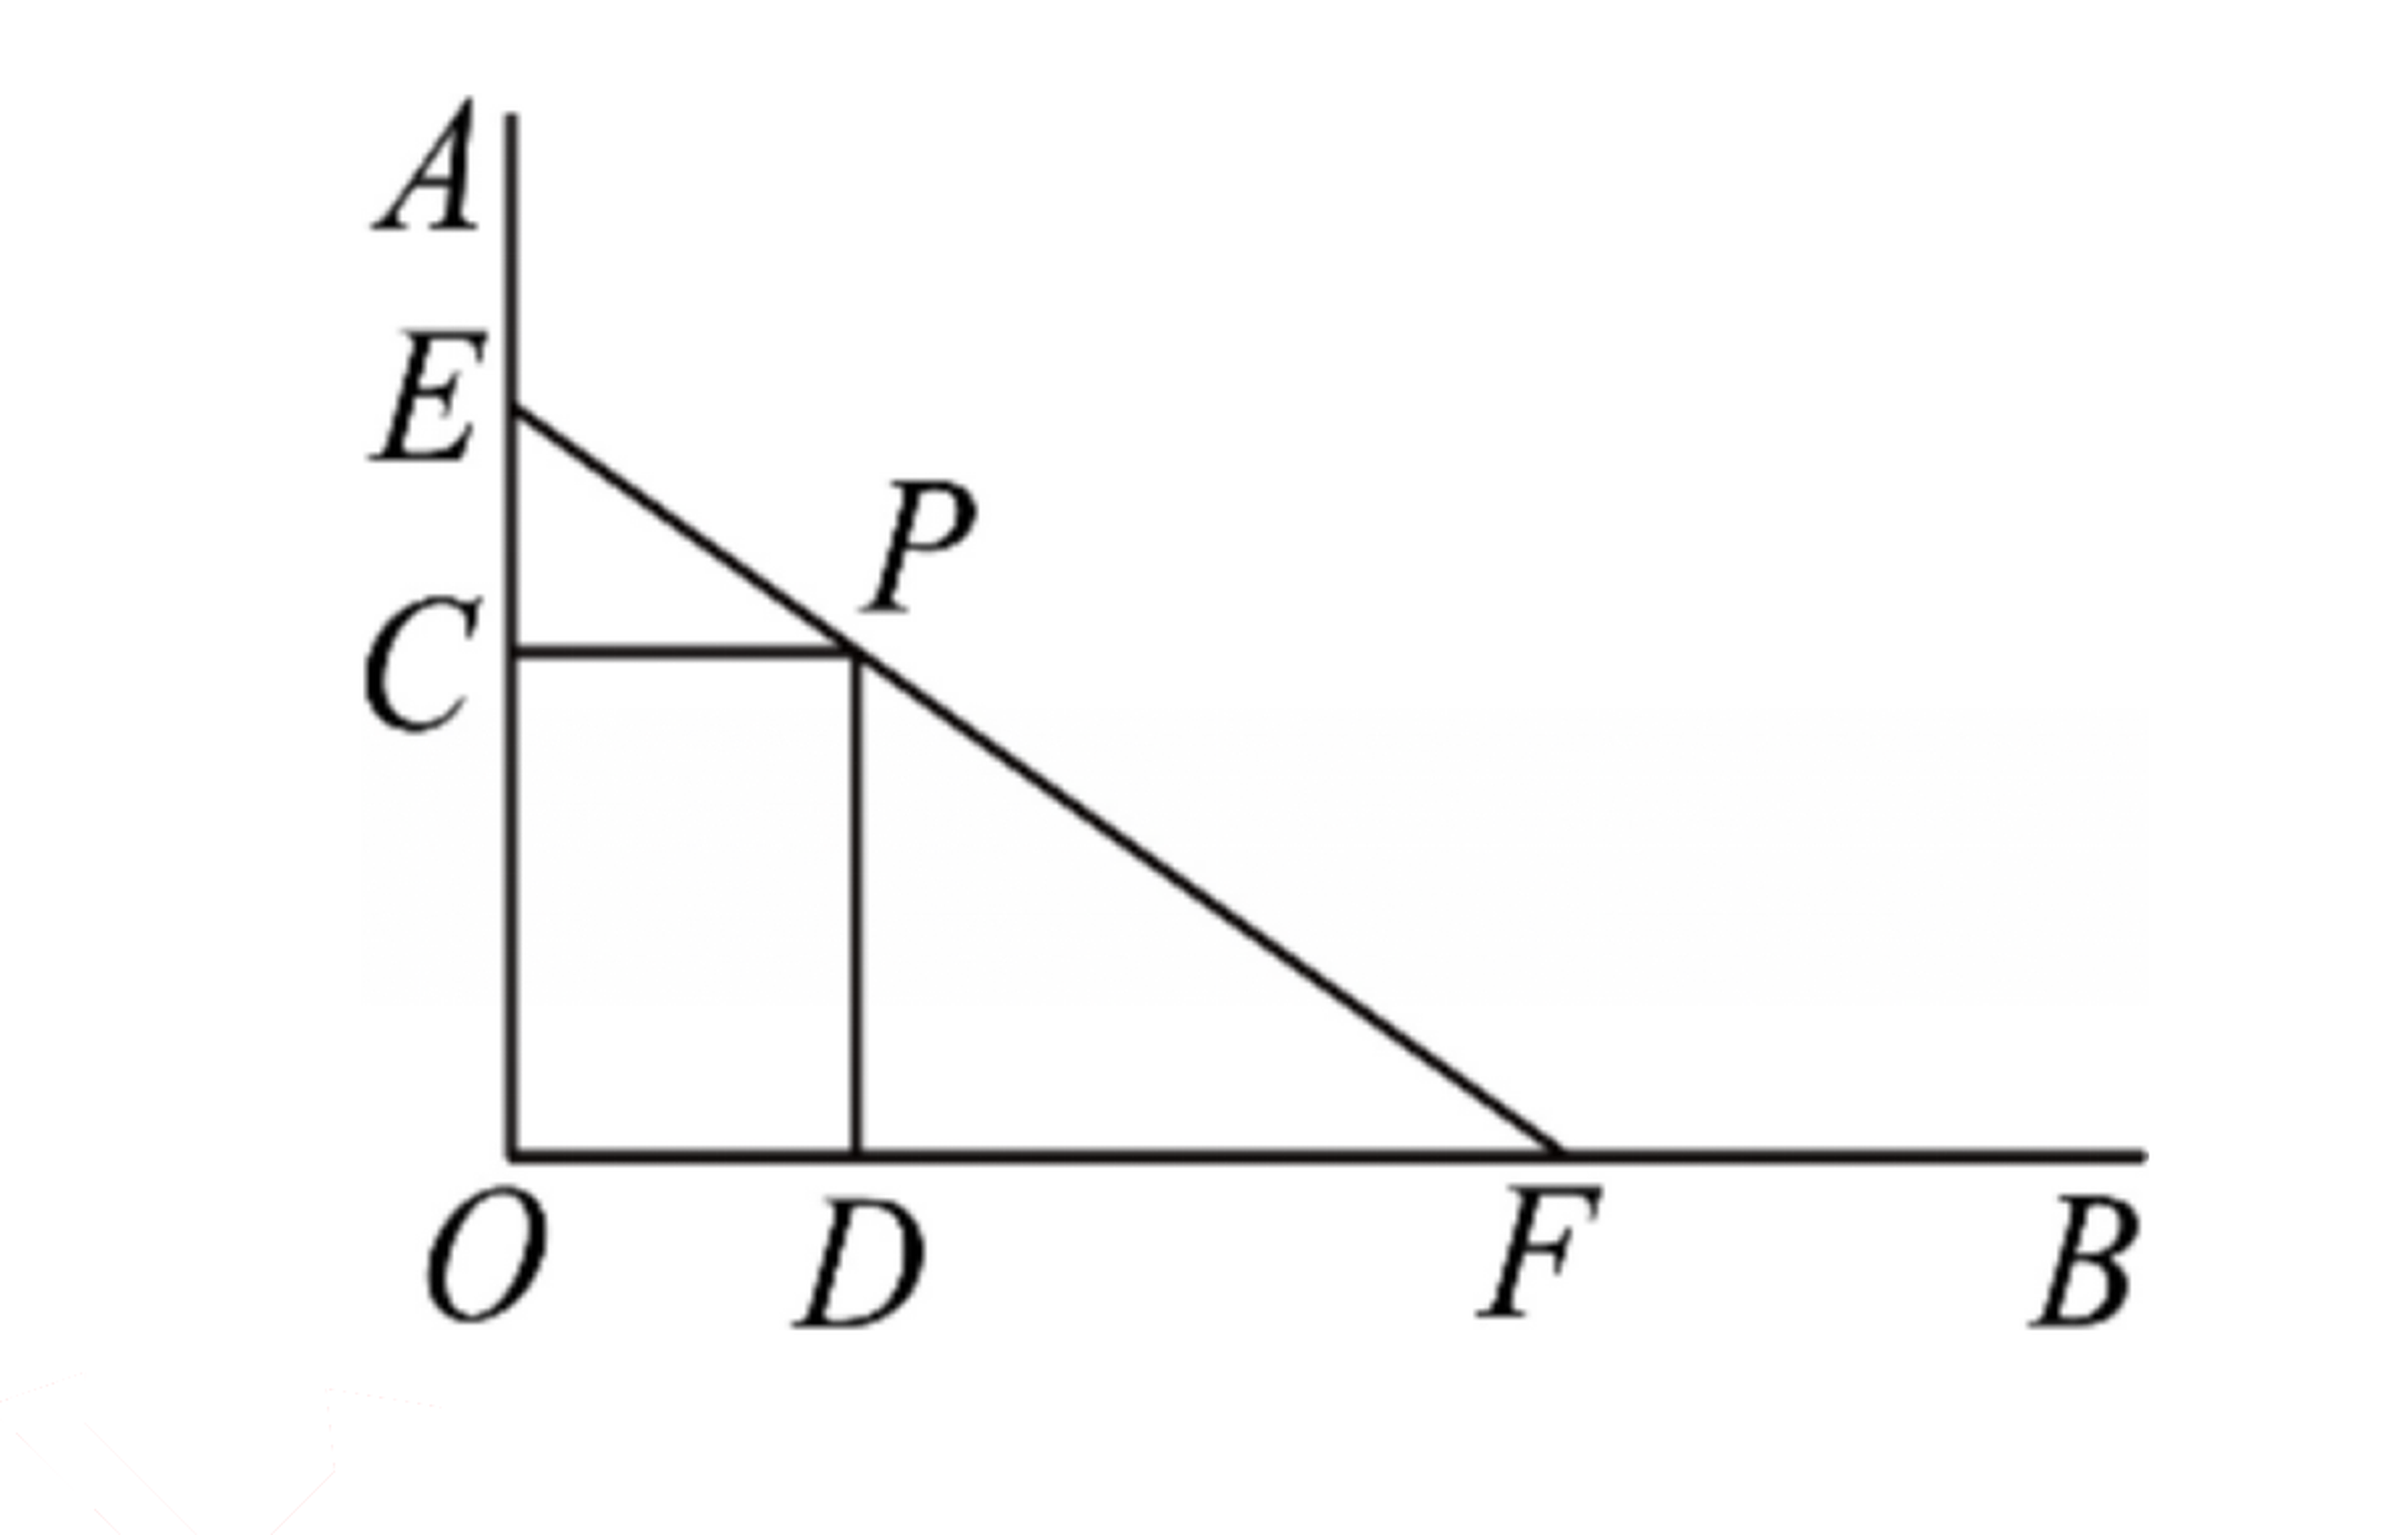
\includegraphics[width=0.32\textwidth]{figures/gao131_q19.png}
\end{center}

\ifanswer
\solbegin
\step{(1) 由题意得 $x\leq60$，}
\step{$\triangle PCE\sim\triangle FDP$，所以 $\dfrac{EC}{CP}=\dfrac{PD}{DF}$，即 $\dfrac{x}{25}=\dfrac{40}{DF}$，得 $DF=\dfrac{1000}{x}$m，}
\step{所以 $OF=OD+DF=\left(25+\dfrac{1000}{x}\right)$m，}
\step{所以 $25+\dfrac{1000}{x}\leq100$，解得 $x\geq\dfrac{40}{3}$；}
\step{综上，$\dfrac{40}{3}\leq x\leq60$；}
\step{(2) 由 $OE=OC+CE=(40+x)$m，}
\step{所以 $S=\dfrac12 OF\cdot OE=\dfrac12\left(25+\dfrac{1000}{x}\right)(40+x)$}
\step{$=\dfrac12\left(1000+25x+\dfrac{40000}{x}+1000\right)$m$^2$，}
\step{由基本不等式得 $S\geq\dfrac12\left(2000+2\sqrt{25x\cdot\dfrac{40000}{x}}\right)=2000$m$^2$，}
\step{当且仅当 $25x=\dfrac{40000}{x}$，即 $x=40$ 时取等号，}
\step{故 $EC=40$m 时，$S$ 取得最小值，为 $2000$m$^2$.}
\solend
\fi

\item 已知 $a\in\R$，函数 $y=ax^2+(3a+2)x+2a+3$.

(1) 当 $a=1$ 时，函数 $y=ax^2+(3a+2)x+2a+3$ 的图象与 $x$ 轴交于 $A(x_1,0)$，$B(x_2,0)$ 两点，求 $x_1^3+x_2^3$；

(2) 若关于 $x$ 的不等式 $ax^2+(3a+2)x+2a+3>2x$ 的解集为 $\R$，求实数 $a$ 的取值范围；

(3) 求关于 $x$ 的不等式 $y\geq1$ 的解集.

\ifanswer
\solbegin
\step{(1) 函数 $y=ax^2+(3a+2)x+2a+3$，当 $a=1$ 时，$y=x^2+5x+5$，}
\step{因为 $y=x^2+5x+5$ 的图象与 $x$ 轴交于 $A(x_1,0)$，$B(x_2,0)$ 两点，}
\step{即 $x^2+5x+5=0$ 的两个根为 $x_1$、$x_2$，}
\step{由根与系数的关系得 $x_1+x_2=-5$，$x_1x_2=5$，}
\step{所以 $x_1^2+x_2^2=(x_1+x_2)^2-2x_1x_2=25-10=15$，}
\step{所以 $x_1^3+x_2^3=(x_1+x_2)(x_1^2+x_2^2-x_1x_2)=-5\times(15-5)=-50$；}
\step{(2) 不等式 $ax^2+(3a+2)x+2a+3>2x$ 恒成立，得 $ax^2+3ax+2a+3>0$.}
\step{当 $a=0$ 时，$3>0$，恒成立，符合题意；}
\step{当 $a\neq0$ 时，若 $a<0$，二次函数 $ax^2+3ax+2a+3$ 开口向下，}
\step{一定存在小于零的部分，故不满足题意；}
\step{当 $a>0$ 时，若使 $ax^2+3ax+2a+3>0$ 恒成立，}
\step{只需 $\Delta=(3a)^2-4\times a\times(2a+3)=a^2-12a<0$，解得 $0<a<12$，}
\step{综上所述，$a$ 的取值范围为 $0\leq a<12$.}
\step{(3) 由 $y\geq1$，得 $ax^2+(3a+2)x+2a+3\geq1$，}
\step{即 $ax^2+(3a+2)x+2a+2\geq0$，即 $(ax+2a+2)(x+1)\geq0$，}
\step{当 $a=0$ 时，$2x+2\geq0$，解得 $x\geq-1$，}
\step{当 $a\neq0$ 时，}
\step{方程 $ax^2+(3a+2)x+2a+2=0$ 即为 $(x+1)(ax+2a+2)=0$，}
\step{解得 $x=-1$ 或 $x=-2-\dfrac2a$，令 $-1=-2-\dfrac2a$，即 $a=-2$，}
\step{当 $a>0$ 时，$-2-\dfrac2a<-1$，}
\step{不等式 $ax^2+(3a+2)x+2a+2\geq0$ 即为 $\left(x+\dfrac{2a+2}a\right)(x+1)\geq0$，}
\step{解得 $x\leq-2-\dfrac2a$ 或 $x\geq-1$；}
\step{当 $a<0$ 时，当 $-2-\dfrac2a<-1$，即 $a<-2$ 时，}
\step{不等式 $ax^2+(3a+2)x+2a+2\geq0$，即为 $\left(x+\dfrac{2a+2}a\right)(x+1)\leq0$，}
\step{解得 $-2-\dfrac2a\leq x\leq-1$；}
\step{当 $-2-\dfrac2a=-1$，即 $a=-2$，}
\step{不等式 $ax^2+(3a+2)x+2a+2\geq0$ 即为 $-2x^2-4x-2\geq0$，解得 $x=-1$，}
\step{当 $-2-\dfrac2a>-1$，即 $-2<a<0$ 时，}
\step{不等式 $ax^2+(3a+2)x+2a+2\geq0$ 即为 $\left(x+\dfrac{2a+2}a\right)(x+1)\leq0$，}
\step{解得 $-1\leq x\leq-2-\dfrac2a$，}
\step{综上所述，当 $a=0$ 时，解集为 $\{x\mid x\geq-1\}$；}
\step{当 $a>0$ 时，解集为 $\{x\mid x\leq-2-\dfrac2a$ 或 $x\geq-1\}$；}
\step{当 $a<-2$ 时，解集为 $\{x\mid -2-\dfrac2a\leq x\leq-1\}$；}
\step{当 $a=-2$ 时，解集为 $\{x\mid x=-1\}$；}
\step{当 $-2<a<0$ 时，解集为 $\{x\mid -1\leq x\leq-2-\dfrac2a\}$.}
\solend
\fi

\item 仔细阅读以下材料：【已知 $a$、$b\in(0,+\infty)$，$a+b=1$，求 $y=\dfrac1a+\dfrac2b$ 的最小值.

$y=\dfrac1a+\dfrac2b=\left(\dfrac1a+\dfrac2b\right)(a+b)=\dfrac ba+\dfrac{2a}b+3\geq3+2\sqrt2$，当且仅当 $\dfrac ba=\dfrac{2a}b$，即 $a=\sqrt2-1$，$b=2-\sqrt2$ 时取得等号，则 $y=\dfrac1a+\dfrac2b$ 的最小值为 $3+2\sqrt2$.

另 $y=\dfrac1a+\dfrac2b=\dfrac{a+b}a+\dfrac{2(a+b)}b=\dfrac ba+\dfrac{2a}b+3\geq3+2\sqrt2$，当且仅当 $\dfrac ba=\dfrac{2a}b$，即 $a=\sqrt2-1$，$b=2-\sqrt2$ 时取得等号，则 $y=\dfrac1a+\dfrac2b$ 的最小值为 $3+2\sqrt2$.】参考上述解法，求解下列问题.

(1) 若正实数 $x$、$y$ 满足 $x+y=1$，求 $\dfrac2x+\dfrac3y$ 的最小值；

(2) 已知 $x\in\left(0,\dfrac12\right)$，求 $t=\dfrac1x+\dfrac8{1-2x}$ 的最小值，并写出此时 $x$ 的值；

(3) 已知 $a$、$b\in(0,+\infty)$，$a+2b=1$，求 $p=\dfrac1{3a+4b}+\dfrac1{a+3b}$ 的最小值.

\ifanswer
\solbegin
\step{(1) 因为 $x>0,y>0$，且 $x+y=1$，}
\step{所以 $\dfrac2x+\dfrac3y=\left(\dfrac2x+\dfrac3y\right)(x+y)=2+\dfrac{2y}x+\dfrac{3x}y+3=5+\dfrac{2y}x+\dfrac{3x}y$，}
\step{由基本不等式得 $\dfrac{2y}x+\dfrac{3x}y\geq2\sqrt{\dfrac{2y}x\cdot\dfrac{3x}y}=2\sqrt6$，}
\step{当且仅当 $\dfrac{2y}x=\dfrac{3x}y$，即 $2y^2=3x^2$ 时，等号成立，}
\step{又因为 $x>0,y>0$ 且 $x+y=1$，此时 $x=\sqrt6-2,y=3-\sqrt6$，}
\step{所以 $\dfrac2x+\dfrac3y\geq5+2\sqrt6$，故 $\dfrac2x+\dfrac3y$ 的最小值为 $5+2\sqrt6$.}
\step{(2) 由 $0<x<\dfrac12$，则 $t=\dfrac1x+\dfrac8{1-2x}=\dfrac{2(1-2x+2x)}{2x}+\dfrac{8(1-2x+2x)}{1-2x}$}
\step{$=10+\dfrac{2\cdot(1-2x)}{2x}+\dfrac{8\cdot2x}{1-2x}\geq10+2\sqrt{\dfrac{2\cdot(1-2x)}{2x}\cdot\dfrac{8\cdot2x}{1-2x}}=18$，}
\step{当且仅当 $\dfrac{2\cdot(1-2x)}{2x}=\dfrac{8\cdot2x}{1-2x}$，即 $x=\dfrac16$ 时等号成立；}
\step{(3) 由 $a$、$b>0$，$a+2b=1$，则 $a=1-2b>0$，即 $0<b<\dfrac12$，}
\step{所以 $p=\dfrac1{3a+4b}+\dfrac1{a+3b}=\dfrac1{3a+6b-2b}+\dfrac1{a+2b+b}=\dfrac1{3-2b}+\dfrac1{1+b}$}
\step{$=\dfrac1{3-2b}+\dfrac2{2+2b}$，显然 $3-2b$、$2+2b>0$，}
\step{所以 $p=\dfrac15\cdot(3-2b+2+2b)\cdot\left(\dfrac1{3-2b}+\dfrac2{2+2b}\right)=\dfrac15\left[3+\dfrac{2+2b}{3-2b}+\dfrac{2(3-2b)}{2+2b}\right]$}
\step{$\geq\dfrac15\left[3+2\sqrt{\dfrac{2+2b}{3-2b}\cdot\dfrac{2(3-2b)}{2+2b}}\right]=\dfrac{3+2\sqrt2}5$，}
\step{当且仅当 $\dfrac{2+2b}{3-2b}=\dfrac{2(3-2b)}{2+2b}$，}
\step{即 $b=\dfrac{8-5\sqrt2}2$，$a=5\sqrt2-7$ 时等号成立.}
\solend
\fi

\end{enumerate}

\end{document}
